\documentclass[11pt,oneside]{book}
\usepackage{fontspec}
\setmainfont{Noto Serif}
\setsansfont{Noto Sans}
\setmonofont{Noto Sans Mono}
\newfontfamily\proseunicodefont{DejaVu Serif}
\usepackage[margin=1in]{geometry}
\usepackage{microtype}
\usepackage{amsmath,amssymb,amsthm,mathtools,bm}
\usepackage{graphicx}
\usepackage{adjustbox}
\usepackage{xcolor}
\usepackage{booktabs}
\usepackage{array}
\usepackage{longtable}
\usepackage{enumitem}
\usepackage{float}
\usepackage{caption}
\usepackage{hyperref}
\usepackage{fancyhdr}
\usepackage{tikz}
\usetikzlibrary{arrows.meta,positioning,calc,decorations.pathmorphing}

\hypersetup{
  colorlinks=true,
  linkcolor=blue!50!black,
  urlcolor=blue!50!black,
  citecolor=blue!50!black
}

\setlength{\parskip}{0.5em}
\setlength{\parindent}{0pt}
\setlist[itemize]{topsep=0.25em,itemsep=0.2em}
\setlist[enumerate]{topsep=0.25em,itemsep=0.2em}
\setlength{\headheight}{40pt}
\numberwithin{equation}{chapter}

\newtheorem{theorem}{نظرية}[chapter]
\newtheorem{proposition}[theorem]{قضية}
\newtheorem{lemma}[theorem]{لمّة}
\newtheorem{corollary}[theorem]{نتيجة}
\theoremstyle{definition}
\newtheorem{definition}[theorem]{تعريف}
\newtheorem{example}[theorem]{مثال}
\theoremstyle{remark}
\newtheorem{remark}[theorem]{ملاحظة}

\providecommand{\ket}[1]{\left\lvert#1\right\rangle}
\providecommand{\bra}[1]{\left\langle#1\right\rvert}
\providecommand{\braket}[2]{\left\langle#1\,\middle|\,#2\right\rangle}
\providecommand{\expect}[1]{\left\langle#1\right\rangle}
\newcommand{\lectureoverview}[1]{\paragraph{نظرة عامة.} #1}

\makeatletter
\newcommand{\course@headerfont}{\normalfont\small\itshape}
\newcommand{\course@pagefont}{\normalfont\small}
\newcommand{\course@headerraise}{14pt}
\newlength{\course@headerboxheight}
\setlength{\course@headerboxheight}{\dimexpr\headheight-\course@headerraise-9pt\relax}
\newcommand{\course@leftheadbox}[1]{%
  \raisebox{\course@headerraise}{%
    \parbox[t][\course@headerboxheight][t]{0.82\textwidth}{%
      \raggedright\course@headerfont\strut\MakeUppercase{#1}\strut%
    }%
  }%
}
\newcommand{\course@rightheadbox}[1]{%
  \raisebox{\course@headerraise}{%
    \parbox[t][\course@headerboxheight][t]{0.82\textwidth}{%
      \raggedleft\course@headerfont\strut\MakeUppercase{#1}\strut%
    }%
  }%
}
\renewcommand{\chaptermark}[1]{\markboth{\MakeUppercase{\chaptername\ \thechapter.\ #1}}{}}
\renewcommand{\sectionmark}[1]{\markright{\MakeUppercase{\thesection\hspace{0.4em}#1}}}
\fancyhf{}
\fancyhead[L]{\course@leftheadbox{\leftmark}}
\fancyhead[R]{\course@pagefont\thepage}
\renewcommand{\headrulewidth}{0.5pt}
\pagestyle{fancy}
\fancypagestyle{plain}{%
  \fancyhf{}
  \fancyhead[L]{\course@leftheadbox{\leftmark}}
  \fancyhead[R]{\course@pagefont\thepage}
  \renewcommand{\headrulewidth}{0.5pt}
}
\makeatother

% Video2Book editorial provenance macros
\newenvironment{classroomqa}{%
  \par\medskip\noindent\begin{minipage}{\linewidth}\small\hrule\medskip
}{%
  \medskip\hrule\end{minipage}\par\medskip
}
\newcommand{\audiencequestion}[1]{\noindent\textbf{سؤال من الحضور.} #1\par\smallskip}
\newcommand{\lecturerresponse}[1]{\noindent\textbf{الإجابة.} #1\par}
\newcommand{\lecturetimestamp}[1]{\footnote{التوقيت في المحاضرة: #1.}}
\newcommand{\lectureframe}[1]{\par\smallskip{\centering\footnotesize\itshape لقطة المحاضرة: #1.\par}}
\newcommand{\editorialnote}[1]{\footnote{توضيح تحريري: #1}}

\usepackage{polyglossia}
\setdefaultlanguage{arabic}
\usepackage{sectsty}
\setotherlanguage{english}
\newfontfamily\arabicfont[Script=Arabic]{Amiri}
\newfontfamily\arabicfontsf[Script=Arabic]{Amiri}
\newfontfamily\arabicfonttt[Script=Arabic]{DejaVu Sans Mono}
\let\arabicsectionnumber\thesection
\let\arabicsubsectionnumber\thesubsection
\renewcommand{\thesection}{\LRE{\arabicsectionnumber}}
\renewcommand{\thesubsection}{\LRE{\arabicsubsectionnumber}}
\renewcommand{\contentsname}{المحتويات}
\renewcommand{\chaptername}{الفصل}
\renewcommand{\figurename}{الشكل}
\renewcommand{\tablename}{الجدول}
\renewcommand{\proofname}{البرهان}
\renewcommand{\bibname}{المراجع}
\sectionfont{\raggedleft}
\subsectionfont{\raggedleft}
\makeatletter
\renewcommand{\@pnumwidth}{2.2em}
\renewcommand{\@tocrmarg}{3.2em}
\makeatother
\usepackage{tocloft}
\renewcommand{\cftchapfont}{\small\bfseries}
\renewcommand{\cftchappagefont}{\small\bfseries}
\renewcommand{\cftsecfont}{\small}
\renewcommand{\cftsecpagefont}{\small}
\setlength{\cftsecnumwidth}{3em}
\renewcommand{\cftsubsecfont}{\small}
\renewcommand{\cftsubsecpagefont}{\small}
\setlength{\cftsubsecindent}{4.5em}
\setlength{\cftsubsecnumwidth}{4em}
\emergencystretch=6em
\pdfstringdefDisableCommands{\def\proseunicodefont{}}

\geometry{paperwidth=177.6mm,paperheight=252mm,left=16mm,right=16mm,
 top=18mm,bottom=18mm,includeheadfoot,headheight=28pt,headsep=7mm,footskip=9mm}
\usepackage{scrextend}
\changefontsizes[17pt]{12pt}
\raggedbottom
\renewenvironment{classroomqa}{\par\medskip\begingroup}{\par\endgroup\medskip}
\fancyhf{}
\setlength{\headwidth}{\textwidth}
\fancyhead[L]{\parbox{\textwidth}{\raggedleft\fontsize{9}{11}\selectfont\nouppercase{\leftmark}}}
\fancyfoot[C]{\small\thepage}
\renewcommand{\headrulewidth}{0.3pt}
\fancypagestyle{plain}{\fancyhf{}\fancyfoot[C]{\small\thepage}\renewcommand{\headrulewidth}{0pt}}

\graphicspath{{../../../generated_course_notes/supplementary/advanced_quantum_mechanics/2013_fall/figures/}{../../../generated_course_notes/supplementary/advanced_quantum_mechanics/2013_fall/assets/}}
\begin{document}
\frontmatter
\hypersetup{pageanchor=false}
\begin{titlepage}
\hyphenpenalty=10000\exhyphenpenalty=10000
\thispagestyle{empty}
\begin{tikzpicture}[remember picture,overlay]
  \node[anchor=center,inner sep=0] at (current page.center) {%
    \includegraphics[height=\paperheight,keepaspectratio]{../../../generated_course_notes/supplementary/advanced_quantum_mechanics/2013_fall/assets/cover-art.png}%
  };
  \node[
    anchor=north west,
    align=right,
    text width=0.78\paperwidth,
    fill=white,
    fill opacity=0.9,
    rounded corners=8pt,
    inner xsep=10pt,
    inner ysep=8pt
  ] at ([xshift=0.08\paperwidth,yshift=-0.06\paperheight]current page.north west) {%
    {\fontsize{30}{33}\selectfont\bfseries\color{black!88} \RLE{ميكانيكا الكم المتقدمة}\\[0.85em]}
    {\large\color{black!72} \RLE{النسخة العربية / خريف 2013}}
  };
  \node[
    anchor=south west,
    align=right,
    text width=0.68\paperwidth,
    fill=white,
    fill opacity=0.82,
    text opacity=1,
    rounded corners=6pt,
    inner sep=12pt
  ] at ([xshift=0.08\paperwidth,yshift=0.08\paperheight]current page.south west) {%
    {\normalsize\color{black!78} \RLE{المحاضرات الأصلية: \LRE{Leonard Susskind}}\\[0.35em]}
    {\small\color{black!72} \RLE{النسخة المصاحبة: \LRE{\href{https://lazying.art}{LazyingArt LLC} / \href{https://github.com/lachlanchen/Video2Book}{Video2Book}}}}
  };
\end{tikzpicture}
\mbox{}
\end{titlepage}
\hypersetup{pageanchor=true}

\clearpage
\chapter*{حول هذه الملاحظات}
تتبع هذه الملاحظات المصاحبة، التي حُرِّرت على نحو مستقل، محاضرات ليونارد ساسكيند. وقد أُعيد بناؤها انطلاقًا من التفريغات الآلية، والترجمات النصية، ولقطات مختارة من السبورة، ثم دُقِّقت بمقارنتها بالمواد المصدرية المتاحة. وهي ليست مخطوطة أصلية للأستاذ ساسكيند، ولم يراجعها ولم يعتمدها.

أُعِدَّت هذه الطبعة بواسطة \href{https://lazying.art}{LazyingArt LLC} باستخدام سير العمل المفتوح المصدر \href{https://github.com/lachlanchen/Video2Book}{Video2Book}. وتظل التفريغات الآلية متاحةً بصورة منفصلة، وقد تحتوي على أخطاء في التعرّف. وتُشار إلى التوضيحات التحريرية وإعادات البناء غير البسيطة في الحواشي.
\clearpage
\tableofcontents
\mainmatter
\chapter{متجهات الحالة، والتطور الوحدوي، وتناظر الإزاحة}
\providecommand{\ket}[1]{\left\lvert#1\right\rangle}
\providecommand{\bra}[1]{\left\langle#1\right\rvert}

بعد انقطاع دام ربعين دراسيين، تكون مراجعة سريعة لميكانيكا الكم مفيدة. ولا يمكن أن تستغرق الربع الدراسي كله. والموضوع القادم هو تطبيق ميكانيكا الكم على المسائل التي طُوِّرت أصلًا من أجلها: الذرات، والإلكترونات والجسيمات المرتبطة بها، والفوتونات.

تأتي الذرات أولًا. كيف يمكن أن تأتي الذرات قبل الإلكترونات، مع أن الإلكترونات أجزاء من الذرات؟ لا نحتاج في البداية من ميكانيكا الإلكترون إلا إلى القدر الكافي لكتابة المعادلات الأساسية لذرة الهيدروجين. وبعد ذلك يمكن أن تتبعها دراسة أكثر تفصيلًا للجسيمات الشبيهة بالإلكترون. وفي جميع هذه التطبيقات سيكون التناظر أداة متكررة: كيف تُمثَّل التناظرات في ميكانيكا الكم، وما الذي تقتضيه بشأن نظام ما.

\section{الحالات، والمرصودات، والتعامد}

في الميكانيكا الكلاسيكية، تُمثَّل الحالة بنقطة في فضاء الطور. وفي ميكانيكا الكم، تُمثَّل بمتجه في فضاء متجهي مركب. وهذا متجه مجرد، لا سهم في الفضاء الثلاثي الأبعاد العادي. ويمكن جمع متجهات الحالة وضربها في أعداد مركبة، ولا يلزم أن يكون الفضاء الذي يحتويها ذا أي بعد منتهٍ معين.

يكتب ترميز ديراك متجه الحالة على صورة كيت،
\begin{equation}
\ket{\psi},
\end{equation}
ويربط به برا،
\begin{equation}
\bra{\psi}.
\end{equation}
وترتبط البرا والكيت بأخذ المرافق الهرميتي. وضم برا إلى كيت يعطي جداءً داخليًا،
\begin{equation}
\langle\phi|\psi\rangle,
\end{equation}
ويكون هذا عمومًا عددًا مركبًا.

المرصود هو شيء يمكن قياسه: الموضع، أو الزخم، أو الطاقة، أو أي كمية أخرى قابلة للقياس. وفي ميكانيكا الكم يُمثَّل المرصود بمؤثر خطي هرميتي \(A\)،
\begin{equation}
A^\dagger=A.
\end{equation}
والهرميتية هي النظير على مستوى المؤثرات لكون الكمية حقيقية. وعلى وجه الخصوص، فإن القيم الذاتية لمؤثر هرميتي تكون حقيقية.

متجه ذاتي لـ \(A\) يحقق
\begin{equation}
A\ket{\alpha}=\alpha\ket{\alpha}.
\end{equation}
والقيم الذاتية الممكنة هي النتائج الممكنة لقياس \(A\). فإذا كان مرصود ما لا يمكن أن يعطي إلا \(1\)، أو \(3\)، أو \(7\)، فإن هذه الأعداد هي قيمه الذاتية. أما متجهاته الذاتية فهي الحالات التي تكون فيها النتيجة محددة لا إحصائية. وفي الحالة \(\ket{\alpha}\)، فإن قياس \(A\) يعطي \(\alpha\) على وجه اليقين.

يعبِّر الجداء الداخلي عن علاقة منطقية مهمة بين الحالات. افترض وجود قياس يميز \(\ket{\phi}\) عن \(\ket{\psi}\) على وجه اليقين. عندئذ تكون الحالتان متعامدتين:
\begin{equation}
\langle\phi|\psi\rangle=0.
\end{equation}
ويعني التعامد أن الحالتين يمكن تمييزهما فيزيائيًا بلا لبس. ولحالة مطبَّعة،
\begin{equation}
\langle\psi|\psi\rangle=1.
\end{equation}

\section{جسيم في تمثيل الموضع}

لننظر أولًا في جسيم يتحرك على مستقيم. موضعه \(x\) مرصود. ولكل موضع ممكن \(x_0\)، توجد حالة \(\ket{x_0}\) يكون فيها قياس الموضع معطيًا يقينًا \(x_0\).

الحالات المرتبطة بمواضع مختلفة قابلة للتمييز، ومن ثم فهي متعامدة:
\begin{equation}
x\neq x'
\quad\Longrightarrow\quad
\langle x'|x\rangle=0.
\end{equation}
ولحالة اعتباطية \(\ket{\psi}\)، يعرِّف تراكبها مع حالة موضع الدالة الموجية:
\begin{equation}
\psi(x)=\langle x|\psi\rangle.
\end{equation}
وهذا هو تمثيل الموضع لمتجه الحالة.

الدالة الموجية ليست هي نفسها احتمالًا. يمكن أن تكون موجبة، أو سالبة، أو تخيلية، أو مركبة عمومًا. وكثافة احتمال الموضع هي
\begin{equation}
P(x)=\psi^*(x)\psi(x)=|\psi(x)|^2.
\end{equation}
وهذا الجداء غير سالب، كما يجب لكثافة الاحتمال. وللدالة الموجية المطبَّعة،
\begin{equation}
\int_{-\infty}^{\infty}dx\,|\psi(x)|^2=1.
\end{equation}

في تمثيل الموضع، يؤثر مؤثر الموضع بالضرب:
\begin{equation}
(\hat x\psi)(x)=x\psi(x).
\end{equation}
ودواله الذاتية دوال مثالية متمركزة في نقطة واحدة. وتوصَف صوريًا بأنها دوال دلتا لديراك: قمم ضيقة جدًا متمركزة عند القيمة الذاتية للموضع. وليس تعريفها التوزيعي الدقيق مطلوبًا في هذه المراجعة الحالية.

في ثلاثة أبعاد، للموضع ثلاث مركبات، \(x\) و\(y\) و\(z\)، وتمثل حالة الموضع نقطة في الفضاء الثلاثي الأبعاد. وتكون حالتان من هذا النوع متعامدتين كلما اختلفت النقطتان في إحداثي واحد على الأقل. وسيُحتفَظ عادةً بالترميز أحادي البعد، مع فهم التعميم الثلاثي الأبعاد المناظر.

\section{الزخم وحالات الزخم المحدد}

يقابل كل مركبة من مركبات الموضع مركبة مناظرة من الزخم. وفي تمثيل الموضع يكون مؤثر الزخم على طول محور \(x\) هو
\begin{equation}
\hat p_x=-i\hbar\frac{d}{dx}.
\end{equation}
وهكذا يمكن أيضًا النظر إلى مؤثر هرميتي مجرد على نحو ملموس بوصفه عملية على الدوال الموجية.

الحالة ذات الزخم المحدد \(p_0\) تحقق معادلة القيم الذاتية
\begin{equation}
\hat p_x\psi_{p_0}(x)=p_0\psi_{p_0}(x).
\end{equation}
وبالتعويض عن الصورة التفاضلية لـ \(\hat p_x\) نحصل على
\begin{equation}
-i\hbar\frac{d\psi_{p_0}(x)}{dx}
=p_0\psi_{p_0}(x).
\end{equation}
ومشتقة الدالة الموجية تتناسب مع الدالة الموجية نفسها، لذا يكون الحل ذا صورة أسية:
\begin{equation}
\psi_{p_0}(x)\propto
\exp\left(\frac{ip_0x}{\hbar}\right).
\end{equation}

\begin{classroomqa}
\lecturetimestamp{00:24:26}
\audiencequestion{هل تصدق هذه المعادلة التفاضلية على أي دالة موجية؟}
\lecturerresponse{لا. إنها معادلة القيمة الذاتية لحالة ذات زخم محدد. ومعظم الدوال الموجية لا تحققها؛ فهي تنتقي دوال الزخم الذاتية.}
\end{classroomqa}

التمييز بين حالات الموضع الذاتية وحالات الزخم الذاتية حاد. فدالة الموضع الذاتية متمركزة في نقطة واحدة. أما دالة الزخم الذاتية فتحقق
\begin{equation}
\left|\exp\left(\frac{ip_0x}{\hbar}\right)\right|^2=1.
\end{equation}
ولذلك يكون معيارها ثابتًا على امتداد المستقيم كله. وفي هذا المعنى المثالي، يعني الزخم المحدد لايقينًا كاملًا في الموضع؛ وكذلك يعني الموضع المحدد لايقينًا كاملًا في الزخم. وهذه هي الصورة القصوى لعلاقة الارتياب في الموضع--الزخم.

\begin{classroomqa}
\lecturetimestamp{00:26:36}
\audiencequestion{إذا كان معلومًا أن الزخم هو \(p_0\)، فلماذا لا يزال هناك توزيع احتمالي؟}
\lecturerresponse{الكمية المعروضة تتعلق بقياس الموضع، لا بقياس آخر للزخم. فالزخم والموضع مرصودان مختلفان. وبالنسبة إلى حالة الزخم الذاتية المثالية، فإن سعة الموضع لها معيار ثابت على امتداد المستقيم كله. أما سعات الزخم فتنتمي إلى تمثيل الزخم، وترتبط بالدالة الموجية في الموضع بتحويل فورييه.}
\end{classroomqa}

\begin{classroomqa}
\lecturetimestamp{00:28:02}
\audiencequestion{كيف تبدو كثافة احتمال الموضع عندما تكون الدالة الموجية دالة دلتا لديراك؟}
\lecturerresponse{إنها متمركزة عند الموضع المحدد. وتعبر القمة المثالية عن اليقين في الموضع.}
\end{classroomqa}

\editorialnote{حالات القيم الذاتية الدقيقة للموضع والزخم هي حالات معمَّمة. ودالة دلتا لديراك وموجة مستوية ليستا دالتين موجيتين عاديتين قابلتين للتكامل تربيعيًا ومطبعتين على المستقيم كله، ومربع دالة دلتا بمعناه الحرفي ليس توزيعًا عاديًا. وتتعلق العبارات أعلاه بتمركزهما المثالي وثبات معيارهما.}

يمكن النظر إلى الدالة الموجية صوريًا على أنها متجه له مركبة واحدة لكل قيمة من قيم \(x\). لكنها، بخلاف متجه عمودي منتهٍ عادي، تملك عددًا لا نهائيًا متصلًا من المركبات.

\begin{classroomqa}
\lecturetimestamp{00:28:53}
\audiencequestion{هل تُمثَّل متجهات الحالة بمتجهات عمودية؟}
\lecturerresponse{يمكن تمثيلها على هذا النحو، لكن كتابة دالة موجية موضعية على شكل عمود عادي غير مريحة لأن \(x\) يأخذ عددًا متصلًا من القيم. ويمكن النظر إليها صوريًا بوصفها متجهًا عموديًا متصلًا، مع اعتبار البرا الموافق متجه صف متصلًا.}
\end{classroomqa}

\section{التطور الزمني والوحدوية}

كيف تتغير الحالة مع الزمن؟ التطور الزمني هو تحويل على فضاء الحالات. ولْيَدُلَّ \(U(t)\) على التطور خلال زمن منقضٍ مقداره \(t\). إذًا
\begin{equation}
U(t)\ket{\psi(t_1)}=\ket{\psi(t_1+t)}.
\end{equation}
وعلى وجه الخصوص،
\begin{equation}
\ket{\psi(t)}=U(t)\ket{\psi(0)},
\qquad
U(0)=\mathbf 1.
\end{equation}

ينتج الشرط على \(U(t)\) من حفظ المعلومات. فإذا كانت حالتان ابتدائيتان قابلتين للتمييز، فلا بد ألا يمحو التطور الزمني ذلك التمييز. ويجب أن تظل الحالات المتعامدة متعامدة. وعلى نحو أعم، يُحفَظ الجداء الداخلي بين أي حالتين:
\begin{equation}
\langle U(t)\phi|U(t)\psi\rangle
=\langle\phi|\psi\rangle.
\end{equation}
وبما أن
\begin{equation}
\langle U(t)\phi|U(t)\psi\rangle
=\langle\phi|U^\dagger(t)U(t)|\psi\rangle,
\end{equation}
فإن حفظ جميع الجداءات الداخلية يقتضي
\begin{equation}
U^\dagger(t)U(t)=\mathbf 1.
\end{equation}
والمؤثر الذي يحقق هذه المعادلة يكون وحدويًا.

\begin{classroomqa}
\lecturetimestamp{00:36:36}
\audiencequestion{هل يُعَدُّ حفظ كل جداء داخلي عبارةً أقوى من مجرد حفظ التعامد؟}
\lecturerresponse{بالنسبة إلى تحويلات الحالات الخطية التي نناقشها، فإن حفظ التعامد يفضي إلى حفظ الجداءات الداخلية. وتقدم الدورانات العادية القياس المألوف: فهي تحفظ التعامد والضرب النقطي.}
\end{classroomqa}

\editorialnote{على وجه التدقيق، فإن حفظ التعامد وحده يسمح بإعادة تحجيم كلية غير صفرية. أما حفظ التطبيع، وهو مطلوب أصلًا للتطور الزمني الفيزيائي، فيزيل تلك الحرية ويعطي حفظ الجداءات الداخلية.}

لا ينبغي الخلط بين المؤثرات الوحدوية والمرصودات الهرميتية. فالموضع والزخم هرميتيان، لكنهما ليسا عمومًا وحدويين. والقيم الذاتية لمؤثر وحدوي هي أطوار، أي أعداد من الصورة \(e^{i\theta}\) تقع على دائرة الوحدة.

\begin{classroomqa}
\lecturetimestamp{00:38:12}
\audiencequestion{ما مثال على تحول غير وحدوي؟}
\lecturerresponse{مؤثرا الموضع والزخم مثالان على ذلك: فهما مؤثران هيرميتيان يمثّلان كميتين قابلتين للرصد، لكنهما ليسا وحدويين. للمؤثر الوحدوي قيم ذاتية معيارها واحد، لذا تكون قيمه الذاتية عوامل طور.}
\end{classroomqa}

\section{الهاملتوني ومعادلة Schr\"odinger}

يُفترض أن التطور الزمني متصل. ولذلك، على فاصل قصير جدًا \(\epsilon\)، لا بد أن يكون مؤثر التطور قريبًا من الهوية:
\begin{equation}
U(\epsilon)=\mathbf 1+\epsilon G+\mathcal O(\epsilon^2).
\end{equation}
وباستخدام الوحدوية،
\begin{align}
U^\dagger(\epsilon)U(\epsilon)
&=
\left(\mathbf 1+\epsilon G^\dagger\right)
\left(\mathbf 1+\epsilon G\right)
+\mathcal O(\epsilon^2)
\\
&=
\mathbf 1+\epsilon(G^\dagger+G)
+\mathcal O(\epsilon^2).
\end{align}
وإلى الرتبة الأولى،
\begin{equation}
G^\dagger=-G.
\end{equation}
إذًا \(G\) مضادّ هيرميتي. ويمكن كتابته على الصورة
\begin{equation}
G=-\frac{i}{\hbar}H,
\end{equation}
حيث إن \(H\) هيرميتي:
\begin{equation}
H^\dagger=H.
\end{equation}
ولذلك يكون مؤثر التطور الزمني المتناهي في الصغر
\begin{equation}
U(\epsilon)
=
\mathbf 1-\frac{i\epsilon}{\hbar}H
+\mathcal O(\epsilon^2).
\end{equation}
والمؤثر الهيرميتي \(H\) هو الهاملتوني.

\begin{classroomqa}
\lecturetimestamp{00:45:48}
\audiencequestion{ما الذي يجيز إهمال الحد \(\epsilon^2\)؟}
\lecturerresponse{يُجرى الحساب باتساق حتى الرتبة الأولى في \(\epsilon\). أما الحساب من الرتبة الثانية فسيتطلب جميع حدود الرتبة الثانية، بما فيها الحد المتناسب مع \(-\epsilon^2H^2/(2\hbar^2)\). يقع التقريب في التعبير المقطوع لـ \(U(\epsilon)\)، لا في هيرميتية \(H\).}
\end{classroomqa}

يمكن بناء فاصل زمني منتهٍ من كثير من الفواصل الصغيرة. اقسم \(t\) إلى \(N\) خطوات طول كل منها \(t/N\). ويعطي تكرار التحول المتناهي في الصغر
\begin{equation}
U(t)
=
\lim_{N\to\infty}
\left(
\mathbf 1-\frac{itH}{N\hbar}
\right)^N
=
\exp\left(-\frac{iHt}{\hbar}\right).
\end{equation}
والأسي هو الصيغة المنتهية للتحول المتناهي في الصغر.

لنطوّر الآن حالة من \(t\) إلى \(t+\epsilon\):
\begin{align}
\ket{\psi(t+\epsilon)}
&=
U(\epsilon)\ket{\psi(t)}
\\
&=
\left(
\mathbf 1-\frac{i\epsilon}{\hbar}H
\right)\ket{\psi(t)}
+\mathcal O(\epsilon^2).
\end{align}
وبطرح \(\ket{\psi(t)}\)، ثم القسمة على \(\epsilon\)، ثم أخذ النهاية، نحصل على
\begin{equation}
\frac{d}{dt}\ket{\psi(t)}
=
-\frac{i}{\hbar}H\ket{\psi(t)}.
\end{equation}
وبصورة مكافئة،
\begin{equation}
i\hbar\frac{d}{dt}\ket{\psi(t)}
=
H\ket{\psi(t)}.
\end{equation}
هذه هي معادلة Schr\"odinger المعتمدة على الزمن. وفي تمثيل الموضع تصبح
\begin{equation}
i\hbar\frac{\partial}{\partial t}\psi(x,t)
=
H\psi(x,t),
\end{equation}
حيث يعمل \(H\) بوصفه مؤثرًا على الدالة الموجية.

معادلة Schr\"odinger المستقلة عن الزمن هي معادلة القيم الذاتية للهاملتوني:
\begin{equation}
H\ket{E}=E\ket{E}.
\end{equation}
والقيم الذاتية \(E\) هي الطاقات الممكن قياسها، أي مستويات الطاقة. ولذا يحدد الهاملتوني نفسه كلًّا من الطاقات المسموح بها وتطور الحالة.

إذا كانت الحالة الابتدائية حالةً ذاتية للطاقة، فإن تطورها هو
\begin{equation}
\ket{E;t}
=
\exp\left(-\frac{iEt}{\hbar}\right)\ket{E}.
\end{equation}
فيبقى متجه الطاقة الذاتي نفسه ولا يكتسب إلا طورًا.\footnote{تتحدد الإشارة السالبة من الاشتقاق السابق لـ \(U(t)=\exp(-iHt/\hbar)\). وفي صياغة منطوقة لاحقة للطور تظهر الإشارة المعاكسة، وهو ما لا يتسق مع ذلك الاشتقاق.}

\begin{classroomqa}
\lecturetimestamp{01:01:05}
\audiencequestion{كيف يتطور متجه ذاتي للطاقة وفق معادلة Schr\"odinger المعتمدة على الزمن؟}
\lecturerresponse{احتفظ بالكيت. بما أن \(H\ket{E}=E\ket{E}\)، فإن التطور الزمني يضرب متجه الطاقة الذاتي بطور تحدده طاقته: \(\exp(-iEt/\hbar)\).}
\end{classroomqa}

\section{ما الذي يُعَدّ تناظرًا؟}

يمثل التطور الزمني أحد التحولات الوحدوية على فضاء الحالات. وتشكل تحولات التناظر فئة مهمة أخرى.

يحتل تناظر الدوران مكانة مركزية في الفيزياء الذرية. ففي ذرة الهيدروجين يتحرك الإلكترون في جهد كولوم المركزي. إن تدوير جهاز الإحداثيات لا يغير المعادلات، كما أن تدوير الذرة نفسها فيزيائيًا يتركها أيضًا ذرة هيدروجين تحكمها المعادلات نفسها. قد تتغير الحالة تحت الدوران، لكن القانون الديناميكي لا يتغير.

يعطي الانسحاب مثالًا آخر. ينبغي أن يسلك نظام معزول في فضاء خالٍ السلوك نفسه بعد أن تُزاح كل أجزائه بالمقدار نفسه. وهذا القيد مهم. فإذا وُجد فرن ونُقل النظام وحده ليصبح أقرب إليه، فقد يسلك النظام سلوكًا مختلفًا؛ فالفرن يكسر تناظر الانسحاب ذاك. أما إذا أُزيح كل من النظام والفرن معًا، فإن العلاقة الأصلية بينهما تُستعاد.

ليست كل عملية تناظرًا. فضغط بلورة من الملح الصخري بمعامل اثنين يغير سلوكها عمومًا. وهذا الضغط تحول محدد جيدًا، لكنه ليس تناظرًا على العموم.

وعليه فالتناظر عملية على الحالات تحفظ صورة الديناميكيات. ولنرمز إليه بـ \(V\). ويجب أن يحفظ قابلية التمييز: فلا بد أن تبقى حالتان متعامدتان متعامدتين بعد التحول. وبناءً على ذلك،
\begin{equation}
V^\dagger V=\mathbf 1,
\end{equation}
ومن ثم فإن \(V\) وحدوي.

\section{التناظرات تتبادل مع التطور الزمني}

افترض أن حالة ابتدائية \(\ket{\psi_1}\) تتطور إلى \(\ket{\psi_2}\):
\begin{equation}
\ket{\psi_2}=U(t)\ket{\psi_1}.
\end{equation}
طبّق تناظرًا مقترحًا \(V\) على كلتا الحالتين:
\begin{equation}
\ket{\psi_1'}=V\ket{\psi_1},
\qquad
\ket{\psi_2'}=V\ket{\psi_2}.
\end{equation}
إذا كان \(V\) تناظرًا للديناميكيات، فلا بد أن تتطور الحالة الابتدائية المحوَّلة إلى الحالة النهائية المحوَّلة:
\begin{equation}
\ket{\psi_2'}=U(t)\ket{\psi_1'}.
\end{equation}
وبالتعويض عن التعريفات نحصل على
\begin{equation}
VU(t)\ket{\psi_1}
=
U(t)V\ket{\psi_1}.
\end{equation}
ويجب أن يصح هذا لكل حالة ابتدائية. لذلك
\begin{equation}
VU(t)=U(t)V.
\end{equation}

يمكن عرض المسارين المتكافئين في مخطط تبادلي.\footnote{يعيد هذا المخطط بناء حجة المسارين المطوَّرة بين 01:10:30 و01:16:34.}
\begin{figure}
\centering
\begin{tikzpicture}[>=Stealth]
\node (a) at (0,0) {$\ket{\psi_1}$};
\node (b) at (4.2,0) {$\ket{\psi_2}=U(t)\ket{\psi_1}$};
\node (c) at (0,-2.0) {$V\ket{\psi_1}$};
\node (d) at (4.2,-2.0) {$V\ket{\psi_2}=U(t)V\ket{\psi_1}$};

\draw[->] (a) -- node[above] {$U(t)$} (b);
\draw[->] (c) -- node[below] {$U(t)$} (d);
\draw[->] (a) -- node[left] {$V$} (c);
\draw[->] (b) -- node[right] {$V$} (d);
\end{tikzpicture}
\caption{يعطي تطبيق تناظر والتطور الزمني الحالة النهائية نفسها في أيٍّ من الترتيبين.}
\end{figure}

\begin{classroomqa}
\lecturetimestamp{01:16:38}
\audiencequestion{هل يجب أن يتبادل التناظر مع التطور الزمني لجميع الأزمنة؟}
\lecturerresponse{نعم. يجب أن يحقق تناظر الديناميكيات شرط التبادل مع التطور الزمني الكامل.}
\end{classroomqa}

\begin{classroomqa}
\lecturetimestamp{01:17:13}
\audiencequestion{هل يعني هذا أنه يمكن إجراء دوران ثم الانتظار، أو الانتظار ثم إجراء دوران؟}
\lecturerresponse{بالضبط. إذا كان الدوران تناظرًا، فإن كلا الترتيبين يعطي الحالة النهائية المحوَّلة نفسها.}
\end{classroomqa}

على فاصل زمني صغير،
\begin{equation}
U(\epsilon)
=
\mathbf 1-\frac{i\epsilon}{\hbar}H
+\mathcal O(\epsilon^2).
\end{equation}
ويصبح شرط التبادل
\begin{equation}
V\left(
\mathbf 1-\frac{i\epsilon}{\hbar}H
\right)
=
\left(
\mathbf 1-\frac{i\epsilon}{\hbar}H
\right)V
+\mathcal O(\epsilon^2).
\end{equation}
وتتلاشى حدود الهوية، ويبقى
\begin{equation}
VH=HV,
\end{equation}
أو
\begin{equation}
[V,H]=0.
\end{equation}
إذًا تكون العملية الوحدوية تناظرًا للديناميكيات إذا وفقط إذا كانت تتبادل مع الهاملتوني.

\begin{classroomqa}
\lecturetimestamp{01:19:29}
\audiencequestion{ما الذي يقتضي أن يكون مؤثر التناظر \(V\) وحدويًا؟}
\lecturerresponse{يجب على التناظر أن يحفظ الفروق المنطقية بين الحالات. فلا ينبغي له أن يحوّل حالتين متنافيتين ومتعامدتين إلى حالتين لا تعودان قابلتين للتمييز. وحفظ تلك العلاقات يتطلب تحولًا وحدويًا.}
\end{classroomqa}

المؤثر الذي لا يملك اعتمادًا زمنيًا صريحًا ويتبادل مع \(H\) يكون محفوظًا. وهذا يربط التناظر بالانحفاظ. وفي الميكانيكا الكلاسيكية تُعبَّر هذه العلاقة بمبرهنة Noether. وفي الصيغة الكمومية الحالية، المعيار الأساسي هو المبدّل مع الهاملتوني.

\section{التناظرات المتقطعة والمستمرة}

يمكن أن تكون التناظرات متقطعة أو مستمرة. فالانعكاس المرآتي متقطع: فهو يبدّل اليسار باليمين، من غير وجود سلسلة من انعكاسات متناهية الصغر بينهما. ويُعدّ تبديل جسيمين متماثلين عملية متقطعة أخرى. كما أن قلب جسم ذي وجهين غير معلَّمين يعطي النوع نفسه من الأمثلة.

أما الدورانات فمستمرة. فدوران بمقدار \(90^\circ\) يمكن بناؤه من كثير من الدورانات الصغيرة حول المحور نفسه. وكذلك الانسحابات المكانية مستمرة للسبب نفسه: إذ يمكن بناء إزاحة منتهية من كثير من الإزاحات الصغيرة جدًا.

إن إمكان تجزئة التحول إلى تحولات صغيرة يمنح التناظرات المستمرة صورة خاصة. وقرب الهوية، نكتب
\begin{equation}
V(\epsilon)
=
\mathbf 1-i\epsilon G+\mathcal O(\epsilon^2),
\end{equation}
حيث يحدد \(\epsilon\) التحول. وتقتضي الوحدوية
\begin{equation}
G^\dagger=G.
\end{equation}
ويُسمّى المؤثر الهيرميتي \(G\) مولِّد التناظر.

إذا كان التحول تناظرًا، فإن
\begin{equation}
[H,V(\epsilon)]=0.
\end{equation}
ويعطي التوسيع إلى الرتبة الأولى
\begin{equation}
[H,G]=0.
\end{equation}
ولذلك تُولَّد التناظرات المستمرة بمؤثرات هيرميتية تتبادل مع الهاملتوني. وهذه المولِّدات كميات محفوظة.

لكلمة ``مولَّدة'' هنا معنى ملموس. فالتحول المنتهي يُبنى بتطبيق التحول المتناهي في الصغر مرارًا، تمامًا كما يُبنى التطور الزمني المنتهي من كثير من الخطوات الزمنية القصيرة.

\section{تناظر الانسحاب والزخم}

اعتبر انسحابًا فعّالًا لدالة موجية إلى اليمين بمسافة \(\epsilon\). فإذا كانت الدالة الموجية الأصلية تتمركز عند \(x_0\)، فينبغي أن تتمركز الدالة الموجية المنساحة عند \(x_0+\epsilon\). ولذلك تكون قيمتها عند الإحداثي \(x\) هي قيمة الدالة الموجية الأصلية المحسوبة عند \(x-\epsilon\):
\begin{equation}
(T(\epsilon)\psi)(x)=\psi(x-\epsilon).
\end{equation}
ولإزاحة صغيرة،
\begin{equation}
\psi(x-\epsilon)
=
\psi(x)-\epsilon\frac{d\psi(x)}{dx}
+\mathcal O(\epsilon^2).
\end{equation}
ومن ثم
\begin{equation}
T(\epsilon)
=
\mathbf 1-\epsilon\frac{d}{dx}
+\mathcal O(\epsilon^2).
\end{equation}
وباستخدام
\begin{equation}
\hat p_x=-i\hbar\frac{d}{dx},
\qquad
\frac{d}{dx}=\frac{i}{\hbar}\hat p_x,
\end{equation}
يصبح الانسحاب المتناهي في الصغر
\begin{equation}
T(\epsilon)
=
\mathbf 1-\frac{i\epsilon}{\hbar}\hat p_x
+\mathcal O(\epsilon^2).
\end{equation}
والانسحاب المنتهي الموافق هو
\begin{equation}
T(\epsilon)
=
\exp\left(-\frac{i\epsilon}{\hbar}\hat p_x\right).
\end{equation}
ومع الاصطلاح \(V(\epsilon)=\mathbf 1-i\epsilon G+\cdots\)، يعطي وسيط الانسحاب ذي الأبعاد
\begin{equation}
G_{\mathrm{trans}}=\frac{\hat p_x}{\hbar}.
\end{equation}
وبصورة مكافئة، يُسمَّى الزخم مولِّد الانسحابات المكانية عندما يُظهَر عامل \(\hbar\) في الأس.

\begin{classroomqa}
\lecturetimestamp{01:34:08}
\audiencequestion{هل فُقدت إشارة سالبة في اشتقاق الانسحاب؟}
\lecturerresponse{المسألة هي الاتجاه الذي يُسنَد إلى الدالة الموجية المنساحة. فالانسحاب الفعّال إلى اليمين يُمثَّل بـ \(\psi(x-\epsilon)\)، لا بـ \(\psi(x+\epsilon)\). ومع هذا التصحيح، \(T(\epsilon)=\mathbf 1-i\epsilon\hat p_x/\hbar+\cdots\).}
\end{classroomqa}

إنَّ ما إذا كان الزخم محفوظًا أم لا يعتمد على الهاملتوني. بالنسبة إلى جسيم حر يتحرك في بعد واحد،
\begin{equation}
H=\frac{\hat p_x^2}{2m}.
\end{equation}
وبما أن كل مؤثر يتبادل مع أي دالة له،
\begin{equation}
[H,\hat p_x]=0.
\end{equation}
فإن هاملتوني الجسيم الحر لا يتغير تحت الانسحابات، ومن ثم يكون \(\hat p_x\) محفوظًا. وفيزيائيًا، يسلك الجسيم السلوك نفسه أيًّا كان الموضع الابتدائي المختار له. وإن إخضاع الشرط الابتدائي لانسحاب لا يفعل سوى إزاحة الحركة بأكملها.

في ثلاثة أبعاد،
\begin{equation}
H
=
\frac{\hat p_x^2+\hat p_y^2+\hat p_z^2}{2m}.
\end{equation}
كل مركبة من مركبات الزخم تتبادل مع \(H\):
\begin{equation}
[H,\hat p_x]=[H,\hat p_y]=[H,\hat p_z]=0.
\end{equation}
يوجد تناظر انسحابي مستقل في كل اتجاه مكاني. والزخم هو في آن واحد الكمية المحفوظة والمولِّد المرتبط بتلك الانسحابات.

الحالة التالية هي التناظر الدوراني. والدورانات أكثر تعقيدًا لأن الدورانات حول محاور مختلفة لا تتبادل عمومًا: فدوران حول \(x\) يتبعه دوران حول \(y\) ليس هو نفسه في الترتيب العكسي. وهذا يؤدي إلى مولدات تناظر غير متبادلة وإلى البنية الزمرية للدورانات.

\chapter{التناظر، والانحلال، وسلالم العزم الزاوي}
\providecommand{\ket}[1]{\left\lvert#1\right\rangle}

\section{التناظرات ومستويات الطاقة المنحلّة}

التناظر هو عملية لا تغيّر الوصف الفيزيائي لمنظومة ما. فهو لا يغيّر الهاملتوني، ولا معادلة Schr\"odinger، ولا الطاقات الممكنة. وإذا كان مؤثر وحدوي \(S\) يمثّل هذه العملية، فإن الثبات يعني
\begin{equation}
S H S^\dagger=H,
\end{equation}
أو بصورة مكافئة
\begin{equation}
[S,H]=0.
\end{equation}

الانسحاب مثال على ذلك. فإذا نقلت ذرة من موضع إلى آخر فلا تتغيّر طاقتها. وهذا صحيح لكل حالة ذرية، لا للحالة الأرضية وحدها. والدوران مثال آخر، وسيكون الموضوع الرئيسي هنا.

إن تبديل جسيمين متماثلين هو أيضًا تناظر. فتسمية إلكترونين بالإلكترون الأول والإلكترون الثاني، أو Harry وFred، لا تجعلهما مختلفين. ولا يمكن لتبديل التسميتين أن يغيّر خواص الذرة.

للبلورة نوع إضافي من تناظر الانسحاب. فإزاحة البلورة كلها عبر الفضاء انسحاب عادي. أمّا في البلورة اللانهائية، فإن الانسحاب بمقدار مسافة شبكية واحدة يعيد أيضًا الترتيب الفيزيائي نفسه. وبصورة مكافئة، يمكن إعادة وسم مواقع الشبكة بإزاحة فهرس كل موقع بمقدار واحد. وتفسد الحدود هذه العبارة الدقيقة في بلورة منتهية، لكنها تصبح تناظرًا جيدًا بعيدًا عن طرفي بلورة طويلة جدًا.

تجانس الفضاء---أي إن كل موضع يشبه أي موضع آخر---هو تناظر الانسحاب. وتماثل الفضاء في جميع الاتجاهات---أي إن كل اتجاه يشبه أي اتجاه آخر---هو تناظر الدوران.

يرتبط الانحلال بالتناظر، لكنه ليس الشيء نفسه. يكون مستوى الطاقة منحلاً عندما تكون هناك أكثر من حالة واحدة لها هذه الطاقة على وجه الدقة. وبالنسبة إلى هاملتوني عام ذي طيف متقطع، فإن المساواة التامة بين مستويين غير مرتبطين ستكون مصادفة لافتة. وحتى الاتفاق إلى جزء واحد من \(10^{15}\) ليس مساواةً تامة. وتشير حالات الانحلال التام عادةً إلى وجود تناظر.

يفضي التناظر أحيانًا إلى الانحلال، ولكن ليس دائمًا. ويبيّن المثال الأول معًا لماذا يمكن أن يحدث ذلك ولماذا قد لا يكفي تناظر واحد وحده.

\section{جسيم على دائرة}

تأمّل خرزة مقيّدة بالحركة على سلك دائري. يمكن وصف موضعها بالإحداثيين الديكارتيين \(x\) و\(y\)، لكن إحداثيًا زاويًا واحدًا يكفي:
\begin{equation}
\psi=\psi(\theta).
\end{equation}
وكثافة احتمال الموضع على الدائرة هي \(\psi^*(\theta)\psi(\theta)\).

يحوِّل دوران فعلي عكس عقارب الساعة بزاوية صغيرة \(\epsilon\) الدالة كما يلي:
\begin{equation}
\psi(\theta)\longrightarrow\psi(\theta-\epsilon).
\end{equation}
ولذلك
\begin{align}
\delta\psi(\theta)
&=\psi(\theta-\epsilon)-\psi(\theta)\\
&=-\epsilon\frac{d\psi}{d\theta}
+\mathcal O(\epsilon^2).
\end{align}

المؤثر
\begin{equation}
L_z=-i\hbar\frac{d}{d\theta}
\end{equation}
هيرميتي على الدوال الموجية الدورية. وهو النظير الزاوي لـ
\begin{equation}
p_x=-i\hbar\frac{d}{dx}.
\end{equation}
ووجود العامل \(i\) أساسي للهيرميتية. وبدلالة \(L_z\)، لدينا
\begin{equation}
\delta\psi
=-\frac{i\epsilon}{\hbar}L_z\psi
+\mathcal O(\epsilon^2),
\end{equation}
ومن ثم فإن مؤثر الدوران متناهي الصغر هو
\begin{equation}
R(\epsilon)
=1-\frac{i\epsilon}{\hbar}L_z
+\mathcal O(\epsilon^2).
\end{equation}
وهذا يحدد \(L_z\) بوصفه مولِّد الدورانات حول المحور العمودي على الدائرة.

\begin{classroomqa}
\lecturetimestamp{00:11:19}
\audiencequestion{ألا ينبغي أن تكون لإحدى العوامل التي تتضمن \(i\) إشارة معاكسة؟}
\lecturerresponse{يؤدي فحص الإشارات إلى العلاقة أعلاه. ومع الاصطلاح \(\psi(\theta)\to\psi(\theta-\epsilon)\) يكون التغيّر \(-\epsilon\,d\psi/d\theta\)، وهو يساوي \(-i\epsilon L_z\psi/\hbar\).}
\end{classroomqa}

لنوجد الآن الحالات الذاتية للعزم الزاوي:
\begin{equation}
L_z\psi=M\psi.
\end{equation}
وبالتعويض بالمؤثر التفاضلي نحصل على
\begin{equation}
-i\hbar\frac{d\psi}{d\theta}=M\psi,
\end{equation}
وحلولها من الشكل
\begin{equation}
\psi(\theta)=C\exp\left(\frac{iM\theta}{\hbar}\right).
\end{equation}

يوجد شرط إضافي لا يظهر في الحركة على خط لانهائي. فالنقطتان \(\theta=0\) و\(\theta=2\pi\) هما النقطة نفسها، ولذلك يجب على الدالة الموجية المدارية الأحادية القيمة أن تحقق
\begin{equation}
\psi(\theta+2\pi)=\psi(\theta).
\end{equation}
وبالنسبة إلى الدالة الذاتية أعلاه، يقتضي ذلك
\begin{equation}
\exp\left(\frac{2\pi iM}{\hbar}\right)=1.
\end{equation}
وعليه،
\begin{equation}
M=m\hbar,
\qquad
m\in\mathbb Z.
\end{equation}
ومن ثم فإن العزوم الزاوية المدارية الممكنة على الدائرة هي
\begin{equation}
\ldots,-2\hbar,-\hbar,0,\hbar,2\hbar,\ldots.
\end{equation}

هل يجب أن تكون للحالة ذات العزم الزاوي \(m\hbar\) الطاقة نفسها التي للحالة ذات العزم الزاوي \(-m\hbar\)؟ يصف \(m\) الموجب والسالب جهتي دوران متعاكستين. والسؤال هو ما إذا كان تناظر الدوران وحده يقتضي أن تكون لهاتين الحركتين طاقة متساوية.

\begin{classroomqa}
\lecturetimestamp{00:22:51}
\audiencequestion{هل يعني استخدام \(\psi(\theta-\epsilon)\) أن الجسيم يتحرك مع عقارب الساعة؟}
\lecturerresponse{لا. فهذا الاصطلاح يحدِّد فقط أيَّ اتجاه يُسمّى الدوران الموجب. وهو يعيّن إشارات الموضع الزاوي والعزم الزاوي، لكنه لا يحدِّد الاتجاه الفعلي الذي يتحرك فيه الجسيم.}
\end{classroomqa}

يوفّر مجال مغناطيسي عمودي على مستوى الدائرة مثالًا مضادًا. إذ يمكنه أن يزيح طاقات العزم الزاوي الموجب والسالب في اتجاهين متعاكسين، ومن ثم يفصل بينهما. وتعتمد إشارة هذا الانزياح على اصطلاحي الشحنة والاتجاه، لكن المهم هو حدوث هذا الانقسام.

يحافظ مثل هذا المجال مع ذلك على الدورانات حول المحور العمودي. ولذلك فهو يبيّن أن تناظر الدوران وحده لا يقتضي
\begin{equation}
E(m)=E(-m).
\end{equation}
وفي غياب هذا الانقسام، قد يشكّل \(m=1\) و\(m=-1\) زوجًا منحلاً، وكذلك قد يشكّل \(m=2\) و\(m=-2\) زوجًا منحلاً. أمّا الحالة \(m=0\) فليس لها قرين متميّز من هذا النوع.

\section{تناظر الانعكاس والزوج \texorpdfstring{\(m,-m\)}{m, -m}}

لنضف تناظر انعكاس متقطعًا. ولتدلّ \(\mathcal M\) على الانعكاس عبر قطر من أقطار الدائرة:
\begin{equation}
(\mathcal M\psi)(\theta)=\psi(-\theta).
\end{equation}
وهو يعكس جهة الدوران:
\begin{equation}
\mathcal M\psi_m=\psi_{-m}.
\end{equation}

إذا كان الانعكاس تناظرًا، فإن
\begin{equation}
[\mathcal M,H]=0.
\end{equation}
وافترض أن
\begin{equation}
H\ket{m}=E_m\ket{m}.
\end{equation}
فينتج من تطبيق \(\mathcal M\)
\begin{align}
H\mathcal M\ket{m}
&=\mathcal M H\ket{m}\\
&=E_m\mathcal M\ket{m}.
\end{align}
وبما أن \(\mathcal M\ket{m}\) هي الحالة ذات العزم الزاوي \(-m\hbar\)، فإن
\begin{equation}
E_{-m}=E_m.
\end{equation}
يحفظ تناظر الدوران العزم الزاوي؛ ويربط تناظر الانعكاس بين القيمتين المتعاكستين. ومعًا يقتضيان أن يكون الزوج منحلاً.

\begin{classroomqa}
\lecturetimestamp{00:29:54}
\audiencequestion{بما أن للنمطين \(m\) و\(-m\) كثافة الاحتمال نفسها، أفيدل ذلك وحده على أن طاقتيهما متساويتان؟}
\lecturerresponse{لا. فالدالتان الموجيتان \(e^{im\theta}\) و\(e^{-im\theta}\) مختلفتان على الرغم من أن مربعي مقداريهما متساويان. ومعادلة القيمة الذاتية للعزم الزاوي تتعلق بالدالة الموجية نفسها، لا بـ \(\psi^*\psi\) وحده. وتقتضي ميكانيكا الكم السعات، لا الاحتمالات وحدها.}
\end{classroomqa}

يحافظ المجال المغناطيسي على الدورانات حول محوره، لكنه يكسر تناظر الانعكاس المستخدم أعلاه.

\begin{classroomqa}
\lecturetimestamp{00:33:05}
\audiencequestion{هل يعكس تناظر الانعكاس المجال المغناطيسي؟}
\lecturerresponse{نعم. فالمجال المغناطيسي متجه محوري. وعند عكس مجال متجه إلى داخل الصفحة يصبح متجهًا إلى خارجها. وبصورة مكافئة، تحمل حلقة تيار وصورتها المرآتية تيارًا في جهتين متعاكستين، وتنتجان مجالين متعاكسين في الاتجاه.}
\end{classroomqa}

يمكن رؤية عدم التبادلية بين الدوران والانعكاس مباشرةً. فعلى دالة ذاتية للعزم الزاوي،
\begin{align}
\mathcal M L_z\psi_m
&=m\hbar\,\psi_{-m},\\
L_z\mathcal M\psi_m
&=-m\hbar\,\psi_{-m}.
\end{align}
ومن ثم
\begin{equation}
[\mathcal M,L_z]\psi_m
=2m\hbar\,\psi_{-m},
\end{equation}
وهذا غير صفري عندما يكون \(m\neq0\). فالدوران ثم الانعكاس ليس العملية نفسها كالانعكاس ثم الدوران.

يتبادل كلا المؤثرين مع \(H\) حين يكون التحويلان كلاهما تناظرين، لكنهما لا يتبادلان أحدهما مع الآخر. وهذا هو النمط المسؤول عن الانحلال.

\begin{classroomqa}
\lecturetimestamp{00:40:28}
\audiencequestion{هل يولِّد أي زوج غير متبادل من نوع Heisenberg، مثل \(x\) و\(p\)، حالات انحلال؟}
\lecturerresponse{ليس على العموم. فلا بد أيضًا أن يكون المؤثران تناظرين: أي يجب أن يتبادلا مع الهاملتوني. وعادةً لا يكون الموضع والزخم محفوظين معًا. ولو كان كلاهما يتبادل مع \(H\)، لأفادت عدم تبادليتهما وجود انحلال.}
\end{classroomqa}

\section{جبر المبدلات للتناظرات}

لنفترض أن \(A\) و\(B\) هما مولِّدان هيرميتيان لتناظرين متصلين:
\begin{equation}
[A,H]=0,
\qquad
[B,H]=0.
\end{equation}
ولا يقتضي شيء في هاتين المعادلتين أن يتبادل \(A\) و\(B\) أحدهما مع الآخر.

إن المبدِّل \([A,B]\) مضادّ للهيرميتية، لذا عرّف مؤثرًا هيرميتيًا
\begin{equation}
C=i[A,B].
\end{equation}
والعوامل العددية والإشارة الكلية لا أهمية لها هنا. والنقطة المهمة هي أن \(C\) يتبادل أيضًا مع الهاملتوني. وحقًّا،
\begin{equation}
[AB,H]
=A[B,H]+[A,H]B=0,
\end{equation}
وبالمثل
\begin{equation}
[BA,H]=0.
\end{equation}
ولذلك
\begin{equation}
[C,H]
=i\bigl([AB,H]-[BA,H]\bigr)=0.
\end{equation}

قد يكون المولِّد الجديد \(C\) مستقلًا عن \(A\) و\(B\)، وقد يكون مجرد تركيب خطي لمولِّدات معروفة من قبل. فإذا كان جديدًا فأضِفه إلى القائمة وشكِّل مبدِّلات أخرى. وقد يستمر تكرار هذه العملية إلى ما لا نهاية، لكنه كثيرًا ما ينغلق بعد عدد منتهٍ من المولِّدات: أي إن كل مبدِّل لاحق يكون تركيبًا خطيًا من تلك الموجودة سلفًا. وهذا النسق المغلق هو جبر مبدِّلات، أو جبر لي.

تشكّل تحويلات التناظر المنتهية زمرة. وتشكّل مولِّداتها متناهية الصغر جبر لي الموافق.

تكتسب حالات الانحلال أهمية لأنها تنظم الأطياف. فإذا كانت لحالتين الطاقة نفسها، فلا يمكن لإحداهما أن تضمحل إلى الأخرى بإصدار فوتون يحمل فرق الطاقة بينهما. وفي التحليل الطيفي الذري يحدِّد ترتيب المستويات وانحلالها الخطوط الطيفية الممكنة. وينطبق المنطق نفسه على الهادرونات المثارة وانتقالاتها.

\begin{classroomqa}
\lecturetimestamp{00:49:07}
\audiencequestion{هل هذه المبدلات نفسها عناصر في زمرة التناظر؟}
\lecturerresponse{المؤثرات التي يدور النقاش حولها هي مولدات. وتشكل المولدات ومبدلاتها جبر مبدلات، أو جبر لي. أما عمليات التناظر المنتهية المبنية من المولدات فهي عناصر الزمرة.}
\end{classroomqa}

إذا كانت جميع مولدات التناظر تتبادل مع بعضها بعضًا، سُمِّي التناظر أبيلِيًّا. وإذا كانت بعض مبدلاتها غير منعدمة، فهو غير أبيلِي.

\begin{classroomqa}
\lecturetimestamp{00:50:25}
\audiencequestion{ما التعريف الأساسي للمولد؟}
\lecturerresponse{خذ تحويل تناظر وحدويًا قريبًا جدًا من الهوية واكتبه على الصورة \(1-i\epsilon G/\hbar+\cdots\). والمؤثر الهيرميتي \(G\) هو مولده. ويؤدي تكرار التحويل المتناهي الصغر الموافق إلى بناء تحويل منتهٍ.}
\end{classroomqa}

\begin{classroomqa}
\lecturetimestamp{00:52:08}
\audiencequestion{ما المقصود بجبر مولدات التناظر؟}
\lecturerresponse{إنه مجموعة من المولدات يمكن جمعها وطرحها وضربها بأعداد عادية وأخذ مبدلاتها. وفي هذا الجبر تؤدي المبدلة دور الضرب، ويعني الانغلاق أن هذه العمليات لا تنتج مولدات خارج المجموعة.}
\end{classroomqa}

\section{الدورانات حول محاور مختلفة}

تمثل الدورانات أهم مثال على تناظر غير أبيلِي. فالدوران حول المحور \(x\) يتبعه دوران حول المحور \(y\) لا يساوي عمومًا إجراءهما بالترتيب المعكوس. وهذا الاختلاف بينهما يرتبط بدوره بدوران حول المحور الثالث.

\begin{classroomqa}
\lecturetimestamp{00:54:22}
\audiencequestion{هل تتبادل الدورانات المتناهية في الصغر رغم أن الدورانات المنتهية لا تتبادل؟}
\lecturerresponse{إنها تختلف عند المرتبة الثانية في زاويتي الدوران الصغيرتين. وهذا يكفي: فبعد فصل هذين المعلمَين الصغيرين، يكون للمولدات نفسها مبدلة غير منعدمة.}
\end{classroomqa}

قبل حساب المبدلات الكمومية، انظر إلى الصورة الكلاسيكية المناظرة. خذ مدارًا كوكبيًا دائريًا يكون فيه الزخم الزاوي عموديًا على مستواه. إن تدوير المدار كله حول المحور \(y\) يعطي مدارًا مسموحًا آخر له الطاقة نفسها تمامًا. غير أن متجه زخمه الزاوي صار الآن ذا مركبة \(x\) مختلفة.

وهكذا يولد الثبات الدوراني تهيئات لها الطاقة نفسها ومركبات مختلفة للزخم الزاوي. وكموميًا، يظهر هذا على هيئة عدم تبادلية بين مولدات الدوران حول محاور مختلفة.

\section{الزخم الزاوي في الإحداثيات الديكارتية}

لننظر أولًا في جسيم يتحرك في المستوى \(xy\)، من دون تقييده بدائرة. تحت دوران صغير عكس اتجاه عقارب الساعة،
\begin{equation}
\delta x=-\epsilon y,
\qquad
\delta y=\epsilon x.
\end{equation}
وبالنسبة إلى الحالة المُدارة فعليًا، تُقيَّم الدالة الموجية المتحولة عند الإحداثيات المدارة دورانًا عكسيًا:
\begin{equation}
\psi_\epsilon(x,y)
=\psi(x+\epsilon y,y-\epsilon x).
\end{equation}
ومن ثم،
\begin{align}
\delta\psi
&=\epsilon\left(
y\frac{\partial}{\partial x}
-x\frac{\partial}{\partial y}
\right)\psi
+\mathcal O(\epsilon^2)\\
&=-\frac{i\epsilon}{\hbar}
\left(xp_y-yp_x\right)\psi
+\mathcal O(\epsilon^2).
\end{align}
لذلك يكون مولد الدورانات حول المحور \(z\)
\begin{equation}
L_z=xp_y-yp_x.
\end{equation}
وهذه هي المركبة \(z\) للمتجه الكلاسيكي المألوف
\begin{equation}
\mathbf L=\mathbf r\times\mathbf p.
\end{equation}
فهو ليس مجرد الزخم الزاوي الميكانيكي؛ بل هو في ميكانيكا الكم المؤثر الذي يولد دورانات الدالة الموجية.\footnote{اختير اصطلاح الدوران الفعال ليتوافق مع التحويل السابق \(\psi(\theta)\mapsto\psi(\theta-\epsilon)\) ومع التعريف النهائي \(L_z=xp_y-yp_x\) بعد الالتباس الوسيط في الإشارة في الاشتقاق الشفهي.}

ويعطي التبديل الدوري \(x\to y\to z\to x\) المركبتين الأخريين.\footnote{تُستعاد صيغتا \(L_x\) و\(L_y\) بتطبيق التبديل الدوري \(x\to y\to z\to x\)، كما نُصَّ عليه صراحة في المحاضرة، على \(L_z=xp_y-yp_x\).}
\begin{align}
L_x&=yp_z-zp_y,\\
L_y&=zp_x-xp_z,\\
L_z&=xp_y-yp_x.
\end{align}

في نظام ثابت تحت الدوران، تتبادل هذه المؤثرات مع الهاملتوني:
\begin{equation}
[H,L_x]=[H,L_y]=[H,L_z]=0.
\end{equation}
ويمثل جسيم في مجال قوة مركزية المثال القياسي. وهذه المعادلات هي انحفاظ الزخم الزاوي بصيغته الكمومية.

\section{جبر لي للزخم الزاوي}

علاقات التبديل القانونية هي
\begin{align}
[x_i,x_j]&=0,\\
[p_i,p_j]&=0,\\
[x_i,p_j]&=i\hbar\,\delta_{ij}.
\end{align}
تتبادل الإحداثيات مع مركبات الزخم العائدة إلى اتجاهات مختلفة. فمثلًا، يتبادل \(x\) مع \(p_y\)، في حين إن \(x\) لا يتبادل مع \(p_x\).

احسب الآن
\begin{equation}
[L_x,L_y]
=
[yp_z-zp_y,\;zp_x-xp_z].
\end{equation}
تنعدم معظم الحدود. أما المساهمتان غير المنعدمتين فهما
\begin{align}
[yp_z,zp_x]&=-i\hbar\,yp_x,\\
[zp_y,xp_z]&=i\hbar\,xp_y.
\end{align}
لذلك
\begin{align}
[L_x,L_y]
&=i\hbar\left(xp_y-yp_x\right)\\
&=i\hbar L_z.
\end{align}
ويعطي التبديل الدوري لرموز الإحداثيات
\begin{align}
[L_x,L_y]&=i\hbar L_z,\\
[L_y,L_z]&=i\hbar L_x,\\
[L_z,L_x]&=i\hbar L_y.
\end{align}

\begin{classroomqa}
\lecturetimestamp{01:14:50}
\audiencequestion{عندما تعطي المبدلة \(L_z\)، هل لا يزال علينا أن نبيّن أن \(L_z\) ليس تركيبًا خطيًا من \(L_x\) و\(L_y\)؟}
\lecturerresponse{نعم. ثمة التزام بإثبات ذلك الاستقلال بدل افتراضه. ولا يُتابَع عند هذه النقطة برهان جبري مباشر.}
\end{classroomqa}

تنغلق المبدلات المعروضة على الفضاء المولد بـ \(L_x\) و\(L_y\) و\(L_z\): فمتى أُدرجت الثلاثة جميعًا، لم تعد المبدلات اللاحقة تنتج أي مؤثر خارج ذلك الفضاء. وهذا هو جبر لي للزخم الزاوي. ومع
\begin{equation}
[H,L_i]=0,
\qquad i=x,y,z,
\end{equation}
تتضمن هذه العلاقات قدرًا كبيرًا من المعلومات عن طيف الطاقة من دون الحاجة إلى حل معادلة Schr\"odinger الزاوية مباشرةً.

تُستخدم استراتيجية جبرية مشابهة في المذبذب التوافقي الكمومي، حيث تولد مؤثرات الخلق والفناء طيفه. وهنا ستغير المؤثرات المناظرة المركبة \(z\) من الزخم الزاوي بدلًا من الطاقة.

إن اختيار المحور \(z\) ليس إلا اختيارًا للتمثيل. وليس ثمة ما يجعل \(z\) مفضلًا فيزيائيًا على \(x\) أو \(y\)، لكن اختيار مركبة واحدة يعطينا أساسًا ملائمًا. اكتب
\begin{equation}
L_z\ket{m}=m\hbar\ket{m}.
\end{equation}
والمطلوب هو تحديد القيم التي يمكن أن يأخذها \(m\) وكيف ترتبط الحالات ذات القيم المختلفة لـ \(m\) بعضها ببعض.

\begin{classroomqa}
\lecturetimestamp{01:24:02}
\audiencequestion{عندما تقارن هذا البناء بالمذبذب التوافقي، هل تقصد المذبذب التوافقي الكمومي؟ فهذا لم يُغطَّ في المحاضرة السابقة.}
\lecturerresponse{نعم، المقارنة مع المذبذب الكمومي. وبرهان الزخم الزاوي الحالي قائم بذاته ولا يتطلب معرفة بالمذبذب. ويمكن لاحقًا قراءة المشابهة في الاتجاه الآخر: فالمذبذب يستخدم طريقة جبرية مشابهة.}
\end{classroomqa}

\section{رفع الزخم الزاوي وخفضه}

عرّف
\begin{equation}
L_+=L_x+iL_y,
\qquad
L_-=L_x-iL_y.
\end{equation}
وتستلزم مبدلات الزخم الزاوي
\begin{equation}
[L_z,L_+]=\hbar L_+,
\qquad
[L_z,L_-]=-\hbar L_-.
\end{equation}

طبّق العلاقة الأولى على حالة ذاتية لـ \(L_z\):
\begin{align}
L_zL_+\ket{m}
&=\left(L_+L_z+[L_z,L_+]\right)\ket{m}\\
&=(m+1)\hbar\,L_+\ket{m}.
\end{align}
فما لم يكن \(L_+\ket{m}=0\)، فإن الناتج حالة ذاتية أخرى لـ \(L_z\)، ولكن بقيمة ذاتية \((m+1)\hbar\). وبالمثل،
\begin{equation}
L_zL_-\ket{m}
=(m-1)\hbar\,L_-\ket{m}.
\end{equation}
إذن فإن \(L_+\) يرفع \(m\) بمقدار واحد و\(L_-\) يخفضه بمقدار واحد.

ابتداءً من أي قيمة ذاتية واحدة، يولد الجبر سلمًا تختلف قيمه بمقادير صحيحة. وقد يستمر هذا السلم بلا نهاية، أو قد ينتهي لأن
\begin{equation}
L_+\ket{m_{\mathrm{top}}}=0
\end{equation}
عند الطرف العلوي و
\begin{equation}
L_-\ket{m_{\mathrm{bottom}}}=0
\end{equation}
عند الطرف السفلي.

\begin{classroomqa}
\lecturetimestamp{01:35:11}
\audiencequestion{ألم يكن الزخم الزاوي قد فُرض بالفعل أن يكون عددًا صحيحًا بحجة الدائرة؟}
\lecturerresponse{تثبت تلك الحجة القيم الصحيحة للزخم الزاوي المداري الممثل بدوال موجية موضعية أحادية القيمة. أما جبر الزخم الزاوي المجرد فيعطي نتيجة أقل تقييدًا: فقد يحتوي السلم إما على قيم صحيحة أو على قيم نصف صحيحة.}
\end{classroomqa}

إذا انتهى سلم ما، فإن الثبات الدوراني يربط بين طرفيه. فدوران بمقدار \(180^\circ\) حول محور عمودي على \(z\) يحول
\begin{equation}
L_z\longrightarrow-L_z.
\end{equation}
ولذلك يجب أن يكون الطيف متناظرًا حول الصفر:
\begin{equation}
m_{\mathrm{bottom}}=-m_{\mathrm{top}}.
\end{equation}
وبما أن القيم المتجاورة تختلف بمقدار واحد، فثمة احتمالان. فإما أن يحتوي السلم على أعداد صحيحة،
\begin{equation}
\ldots,-2,-1,0,1,2,\ldots,
\end{equation}
أو على أنصاف أعداد صحيحة،
\begin{equation}
\ldots,-\frac{5}{2},-\frac{3}{2},-\frac{1}{2},
\frac{1}{2},\frac{3}{2},\frac{5}{2},\ldots,
\end{equation}
وتكون النهايتان حيثما أعطى مؤثر الرفع أو الخفض صفرًا.

وتنتقي حجة أحادية قيمة الدالة الموجية على الدائرة القيم الصحيحة للزخم الزاوي المداري،
\begin{equation}
\mathbf L=\mathbf r\times\mathbf p.
\end{equation}
أما القيم النصف الصحيحة فهي أيضًا فيزيائية، وتخص الزخم الزاوي المغزلي، الذي سيُعالَج على حدة.

وأخيرًا، تكون حالات السلم متساوية في الطاقة عندما يكون الهاملتوني ثابتًا تحت الدوران. افترض
\begin{equation}
H\ket{m}=E\ket{m}.
\end{equation}
وبما أن كل مركبة \(L_i\) تتبادل مع \(H\)، فإن \(L_+\) و\(L_-\) يتبادلان معه أيضًا. ومن ثم
\begin{align}
H L_+\ket{m}
&=L_+H\ket{m}\\
&=E L_+\ket{m}.
\end{align}
وكلما كان \(L_+\ket{m}\neq0\)، كانت للحالة المرفوعة الطاقة نفسها التي للحالة الأصلية. ويعطي الحساب نفسه
\begin{equation}
H L_-\ket{m}=E L_-\ket{m}.
\end{equation}
ولذلك يولد الرفع والخفض عائلة من الحالات ذات قيم ذاتية مختلفة لـ \(L_z\) ولكن بالطاقة نفسها تمامًا. وهذه هي الصلة بين التناظرات غير المتبادلة والانحلال التي جرى تطويرها على امتداد المحاضرة.

\begin{classroomqa}
\lecturetimestamp{01:44:13}
\audiencequestion{هل ترتبط حالات السلم هذه باختيار محاور دوران مختلفة؟}
\lecturerresponse{إنها مترابطة بالدورانات. فالمتجهات الذاتية لـ \(L_x\) أو \(L_y\) هي تراكيب خطية من المتجهات الذاتية المختارة لـ \(L_z\). ويغير تدوير حالة ما مركبات زخمها الزاوي مع إبقاء طاقتها من دون تغيير.}
\end{classroomqa}

إن اختيار \(L_+\) و \(L_-\) ملائم لأن هذين التركيبين يكشفان السلم مباشرةً. وتتكرر هذه الحيلة في ميكانيكا الكم كلها: فعندما يكون جبر المبدلات منغلقًا، فإن مؤثري الرفع والخفض ينظمان غالبًا طيف القيم الذاتية المرتبط به.

\begin{classroomqa}
\lecturetimestamp{01:46:33}
\audiencequestion{ماذا يحدث عندما يؤثر \(L_+\) في الحالة العظمى، وكيف يُعرَّف الطرف العلوي؟}
\lecturerresponse{إنه يعطي صفراً. وهذا هو تعريفه في سُلَّم منتهٍ. وبالمثل، يعطي \(L_-\) صفراً عند الطرف السفلي. ولا يلزم أن يكون السلم المجرَّد منتهيًا. أما حالات الزخم الزاوي الذرية التي سننظر فيها لاحقًا، فعادةً ما نصادف سلالم منتهية.}
\end{classroomqa}

الخطوة التالية هي المضي في تطوير بنية الزخم الزاوي هذه وتطبيقها على الذرات، بما في ذلك الهيدروجين. والمتعددات الدورانية التي وُجدت هنا تفسّر جزءًا من نمط الانحلال؛ ولا تزال ثمة بنية إضافية يتعين تطويرها.

\chapter{متعددات الزخم الزاوي، والحركة الشعاعية، وسُلَّم المهتز}

\section{الاعتماد الزاوي للدالة الموجية}

للجسيم في مجال قوة مركزية موضع شعاعي وإحداثيان زاويان. في الوصف الكلاسيكي، يكون \begin{equation}
\mathbf L=\mathbf r\times\mathbf p
\end{equation} محفوظًا بوصفه متجهًا. ويحدِّد اتجاهه مستوى المدار، مع أن المدار ليس بالضرورة دائريًا.

في ميكانيكا الكم يوصف الجسيم بـ \begin{equation}
\Psi=\Psi(r,\theta,\phi),
\end{equation} ويتعلق الزخم الزاوي باعتماد هذه الدالة الموجية على الزوايا.

في بعدين لا توجد إلا مركبة واحدة للزخم الزاوي، هي مولِّد الدورانات حول المحور العمودي على المستوى: \begin{equation}
L_z=-i\hbar\frac{\partial}{\partial\theta}.
\end{equation} وتحقق دالة ذاتية ذات قيمة ذاتية \(\hbar\ell\) العلاقة \begin{equation}
-i\hbar\frac{\partial}{\partial\theta}\psi(r,\theta)
=\hbar\ell\,\psi(r,\theta).
\end{equation} والإحداثي \(r\) لا يتدخل في هذه المعادلة. ويكون حلها على الصورة \begin{equation}
\psi(r,\theta)=\chi(r)e^{i\ell\theta}.
\end{equation} وبالنسبة إلى دالة موجية مدارية اعتيادية أحادية القيمة، فإن الرجوع إلى النقطة نفسها بعد \(\theta\to\theta+2\pi\) يقتضي أن يكون \(\ell\) عددًا صحيحًا. وقد يؤثر العامل الشعاعي \(\chi(r)\) في الطاقة، لكنه لا يؤثر في هذه القيمة الذاتية للزخم الزاوي.

أما النظير ثلاثي الأبعاد فيفصل الاعتماد الشعاعي عن الدوال المعرفة على الكرة: \begin{equation}
\Psi(r,\theta,\phi)=R(r)Y_{\ell m}(\theta,\phi).
\end{equation} والدوال \(Y_{\ell m}\) هي التوافقيات الكروية. ولن نحتاج هنا إلى صيغها الصريحة. تؤثر الدورانات في العامل الزاوي، بينما تُترك الدالة الشعاعية كما هي.

\section{متعددات الزخم الزاوي المنتهية}

تُحقِّق مركبات الزخم الزاوي العلاقة \begin{equation}
\begin{aligned}
[L_x,L_y]&=i\hbar L_z,\\
[L_y,L_z]&=i\hbar L_x,\\
[L_z,L_x]&=i\hbar L_y.
\end{aligned}
\end{equation} اختر حالات ذاتية لـ \(L_z\)، \begin{equation}
L_z|\ell,m\rangle=\hbar m\,|\ell,m\rangle,
\end{equation} وعرِّف \begin{equation}
L_\pm=L_x\pm iL_y.
\end{equation} فتؤدي المبدِّلات \begin{equation}
[L_z,L_\pm]=\pm\hbar L_\pm
\end{equation} إلى \begin{align}
L_z\bigl(L_\pm|\ell,m\rangle\bigr)
&=\bigl(L_\pm L_z+[L_z,L_\pm]\bigr)|\ell,m\rangle \\
&=\hbar(m\pm1)L_\pm|\ell,m\rangle.
\end{align} وبالتالي يرفع \(L_+\) القيمة \(m\) بمقدار واحد، ويخفضها \(L_-\) بمقدار واحد، ما لم ينعدم المتجه الناتج.

في المتعددة المنتهية توجد حالة عليا وحالة دنيا: \begin{equation}
L_+|\ell,\ell\rangle=0,
\qquad
L_-|\ell,-\ell\rangle=0.
\end{equation} ويرتبط اتجاها \(+z\) و\(-z\) بدوران، لذا يكون الطيف المنتهي متناظرًا حول الصفر. ومن ثم تكون قيمه \begin{equation}
m=-\ell,-\ell+1,\ldots,\ell-1,\ell,
\end{equation} ويكون عدد الحالات \begin{equation}
2\ell+1.
\end{equation} وبما أن القيم المتجاورة تختلف بمقدار واحد، فيمكن أن تكون القيم الطرفية أعدادًا صحيحة أو أنصاف أعداد صحيحة. وتحقق التوافقيات الكروية المدارية الاعتيادية الحالة الصحيحة؛ كما أن جبر الزخم الزاوي المجرَّد يجيز أيضًا متعددات أنصاف الأعداد الصحيحة.

\begin{classroomqa}\lecturetimestamp{00:16:12}\audiencequestion{هل يمكن أن تحتوي متعددة زخم زاوي على عدد لا نهائي من الحالات؟}\lecturerresponse{يمكن تصور هذا الاحتمال، لكنه لن يكون مطلوبًا هنا. فالزخم الزاوي يرفع الطاقة عمومًا عندما تُثبَّت السمات الأخرى للحالة، لذا فإن حالات الزخم الزاوي اللانهائي ليست ذات صلة عند مناقشة الحالات ذات الطاقة المنتهية.}\end{classroomqa}

\section{القيمة المشتركة لـ \texorpdfstring{\(L^2\)}{مربع L}}

المؤثر الذي يقيس مربع مقدار الزخم الزاوي هو \begin{equation}
L^2=L_x^2+L_y^2+L_z^2.
\end{equation} والجداء المرتب لمؤثري السُّلَّم هو \begin{align}
L_-L_+
&=(L_x-iL_y)(L_x+iL_y) \\
&=L_x^2+L_y^2+i[L_x,L_y] \\
&=L_x^2+L_y^2-\hbar L_z.
\end{align} وعليه، \begin{equation}
L^2=L_z^2+\hbar L_z+L_-L_+.
\end{equation} طبِّق هذه المتطابقة على الحالة العليا. وبما أن \(L_+|\ell,\ell\rangle=0\)، فإن \begin{align}
L^2|\ell,\ell\rangle
&=\left(L_z^2+\hbar L_z+L_-L_+\right)|\ell,\ell\rangle \\
&=\hbar^2\left(\ell^2+\ell\right)|\ell,\ell\rangle,
\end{align} ومن ثم \begin{equation}
L^2|\ell,\ell\rangle
=\hbar^2\ell(\ell+1)|\ell,\ell\rangle.
\end{equation} ومربع المقدار ليس \(\hbar^2\ell^2\). والحد الإضافي هو نتيجة لعدم تبديلية مركبات الزخم الزاوي.

وتخص هذه القيمة نفسها كل حالة في المتعددة، لا الحالة العليا وحدها.

\begin{classroomqa}\lecturetimestamp{00:26:08}\audiencequestion{ما الذي يبرهنه التمرين بالضبط لإظهار أن الحالات الأخرى لها القيمة نفسها لـ \(L^2\)؟}\lecturerresponse{أثبت أن \(L^2\) يبادل كل مركبة من مركبات الزخم الزاوي، ومن ثم يبادل \(L_-\). ثم مرِّر \(L^2\) عبر \(L_-\): فإذا كانت للحالة العليا القيمة الذاتية \(\hbar^2\ell(\ell+1)\)، فإن الحالة التالية نزولًا لها القيمة الذاتية نفسها. ويؤدي تكرار الحجة إلى حمل هذه القيمة على امتداد السُّلَّم كله.}\end{classroomqa}

وبالفعل، \begin{equation}
[L^2,L_i]=0,
\qquad i=x,y,z,
\end{equation} ومن ثم \begin{equation}
[L^2,L_\pm]=0.
\end{equation} فعلى سبيل المثال، \begin{align}
L^2\bigl(L_-|\ell,\ell\rangle\bigr)
&=L_-L^2|\ell,\ell\rangle \\
&=\hbar^2\ell(\ell+1)L_-|\ell,\ell\rangle.
\end{align} ومواصلة النزول تعطي \begin{equation}
L^2|\ell,m\rangle
=\hbar^2\ell(\ell+1)|\ell,m\rangle
\end{equation} لكل \(m=-\ell,\ldots,\ell\).

ويعطي الترتيب المعاكس تحليلًا مكافئًا: \begin{align}
L_+L_-
&=(L_x+iL_y)(L_x-iL_y) \\
&=L_x^2+L_y^2-i[L_x,L_y] \\
&=L_x^2+L_y^2+\hbar L_z,
\end{align} ومن ثم \begin{equation}
L^2=L_z^2-\hbar L_z+L_+L_-.
\end{equation}

\begin{classroomqa}\lecturetimestamp{00:32:05}\audiencequestion{هل يمكن تحليل \(L_x^2+L_y^2\) بالترتيب المعاكس باستخدام \(L_+L_-\)؟}\lecturerresponse{نعم. تنعكس إشارة حد \(L_z\). ومع هذا الترتيب، تُطبَّق المتطابقة على الحالة الدنيا التي يُفنيها \(L_-\)، لا على الحالة العليا. وتنتج القيمة الذاتية نفسها \(\hbar^2\ell(\ell+1)\).}\end{classroomqa}

وعليه فإن التوافقيات الكروية تحقق \begin{align}
L^2Y_{\ell m}
&=\hbar^2\ell(\ell+1)Y_{\ell m}, \\
L_zY_{\ell m}
&=\hbar m\,Y_{\ell m}.
\end{align} ولكل قيمة مدارية \(\ell=0,1,2,\ldots\)، توجد \(2\ell+1\) دالة موسومة بـ \(m=-\ell,\ldots,\ell\).

في حالة جهد مركزي، \begin{equation}
[H,L_i]=0.
\end{equation} وعند تثبيت حالة ذاتية شعاعية للطاقة و\(\ell\)، فإن تغيير \(m\) بواسطة \(L_\pm\) لا يغيِّر الطاقة. لذا فإن كل حالة ذاتية شعاعية من هذا النوع تولِّد متعددة مغناطيسية ذات بُعد \(2\ell+1\).

يظهر سُلَّم الزخم الزاوي المداري الصحيح أدناه.\footnote{أُعيد بناء الشكل من مخطط المتعددة ومتطابقات المؤثرات الظاهرة عند \(00{:}35{:}53\) من فيديو المحاضرة.}

\begin{figure}[htbp]\centering
\begin{tikzpicture}[x=1cm,y=0.85cm,>=stealth]
\draw[->] (0,-3.5) -- (0,3.5) node[above] {$m$};

\fill (0,3) circle (2.2pt);
\fill (0,2) circle (2.2pt);
\fill (0,0) circle (2.2pt);
\fill (0,-2) circle (2.2pt);
\fill (0,-3) circle (2.2pt);

\node[left] at (0,3) {$\ell$};
\node[left] at (0,2) {$\ell-1$};
\node[left] at (0,0) {$0$};
\node[left] at (0,-2) {$-\ell+1$};
\node[left] at (0,-3) {$-\ell$};

\node at (0,1) {$\vdots$};
\node at (0,-1) {$\vdots$};

\draw[->] (-1.15,-2.65) -- (-1.15,2.65)
node[midway,left] {$L_+$};
\draw[->] (1.15,2.65) -- (1.15,-2.65)
node[midway,right] {$L_-$};

\node[anchor=west] at (2.1,1.35)
{$L_z|\ell,m\rangle=\hbar m|\ell,m\rangle$};
\node[anchor=west] at (2.1,0.25)
{$L^2|\ell,m\rangle=\hbar^2\ell(\ell+1)|\ell,m\rangle$};
\node[anchor=west] at (2.1,-0.85)
{$L_\pm|\ell,m\rangle\propto|\ell,m\pm1\rangle$};
\end{tikzpicture}\caption{متعددة صحيحة للزخم الزاوي المداري. يغيِّر \(L_+\) و\(L_-\) القيمة \(m\) بمقدار واحد، بينما يبقى \(L^2\) مساويًا لـ \(\hbar^2\ell(\ell+1)\) على امتداد المتعددة.}\lectureframe{00:35:53}\end{figure}

\section{مسألة القوة المركزية}

انظر إلى \begin{equation}
H=\frac{\mathbf p^2}{2m}+V(r),
\end{equation} حيث إن \(V\) يعتمد فقط على البعد عن الأصل. ويقتضي التناظر الدوراني انحفاظ الزخم الزاوي. كلاسيكيًا، يكون لـ \(\mathbf L\) مقدار واتجاه ثابتان، لذا يبقى المدار في مستوى عمودي على \(\mathbf L\). وليس من الضروري أن يكون المدار دائريًا، ولا حتى مغلقًا.

اختر إحداثيات بحيث يكون هذا المستوى المداري الكلاسيكي هو مستوى \(xy\)، وحلّل الزخم إلى مركبتين شعاعية ومماسية: \begin{equation}
\mathbf p^2=p_r^2+p_\theta^2.
\end{equation} وبما أن مقدار الزخم الزاوي هو \begin{equation}
L=r p_\theta,
\end{equation}، فيمكن كتابة المساهمة المماسية على الصورة \begin{equation}
p_\theta^2=\frac{L^2}{r^2}.
\end{equation} ويصبح الهاملتوني \begin{equation}
H=\frac{p_r^2}{2m}+\frac{L^2}{2mr^2}+V(r).
\end{equation} وعند تثبيت \(L\)، فهذه مسألة أحادية البعد في الإحداثي الشعاعي، ذات جهد فعال \begin{equation}
V_{\mathrm{eff}}(r)=\frac{L^2}{2mr^2}+V(r).
\end{equation} ويظهر الهاملتوني الشعاعي على اللوح أدناه.\footnote{إطار المصدر: \texttt{\detokenize{lecture_03_frame_02.png}}، فيديو المحاضرة عند \(00{:}47{:}15\).}

\begin{figure}[htbp]\centering
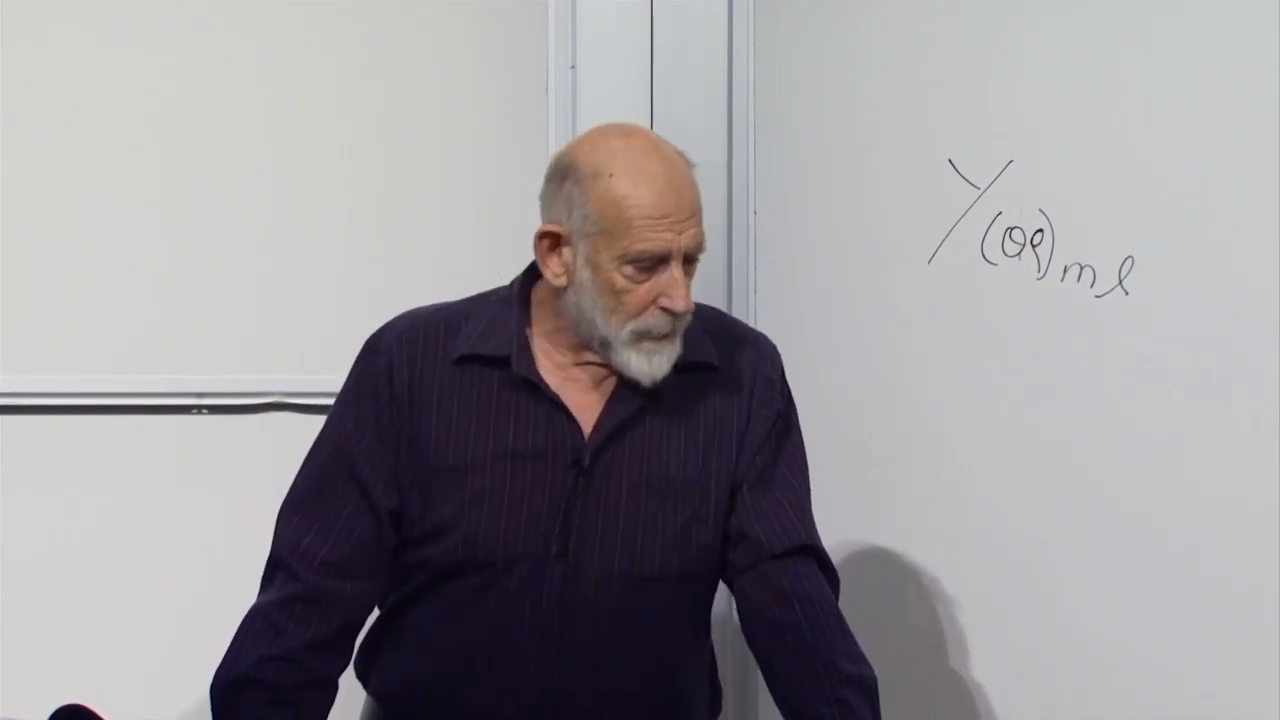
\includegraphics[width=0.9\linewidth]{lecture_03_frame_02.png}\caption{عند تثبيت الزخم الزاوي الكلاسيكي، يحتوي الهاملتوني الشعاعي على طاقة حركة شعاعية، وحد الطرد المركزي \(L^2/(2mr^2)\)، والجهد المركزي \(V(r)\).}\lectureframe{00:47:15}\end{figure}

إن حد \(1/r^2\) هو حاجز الطرد المركزي. فهو يزداد حين يقترب الجسيم من الأصل، ولذلك تتجه القوة المصاحبة إلى الخارج. وبالنسبة إلى تجاذبات شبيهة بكولوم من النوع قيد المناقشة، فإن مسارًا له \(L\neq0\) يلتف حول المركز بدلًا من بلوغه. وعندما يكون \(L=0\)، يغيب هذا الحاجز.

بالنسبة إلى جهد كولوم التجاذبي، \begin{equation}
V(r)=-\frac{\kappa}{r},
\end{equation} يسود حد الطرد المركزي عند القيم الصغيرة لـ \(r\)، بينما يتناقص حد كولوم على نحو أبطأ ويسود عند القيم الكبيرة لـ \(r\). وعندما يكون \(L\neq0\)، يكون لمجموعهما حد أدنى. وتكون الحركة عند هذا الحد الأدنى ذات نصف قطر ثابت، ومن ثم فهي دائرية. أما الحركة المقيدة فوق الحد الأدنى وتحت عتبة الإفلات فتتذبذب بين أصغر نصف قطر وأكبره؛ وفي مسألة كولوم تكون هذه هي الاهتزازات الشعاعية لمدار إهليلجي.

\section{المعادلة الشعاعية المختزلة}

في ميكانيكا الكم يكون الجزء الزاوي من حالة ذات زخم زاوي مداري محدد توافقًا كرويًا. اكتب الحالة المفصولة على الصورة \begin{equation}
\Psi_{n_r\ell m}(r,\theta,\phi)
=\frac{u_{n_r\ell}(r)}{r}\,
Y_{\ell m}(\theta,\phi).
\end{equation} وللمؤثر الزاوي \(L^2\) القيمة الذاتية \begin{equation}
L^2Y_{\ell m}
=\hbar^2\ell(\ell+1)Y_{\ell m}.
\end{equation} ولزوج ثابت \(n_r,\ell\)، اختصر \(u_{n_r\ell}(r)\) إلى \(u(r)\). وتكون المعادلة المتبقية للدالة الشعاعية المختزلة هي \begin{equation}
\begin{aligned}
&-\frac{\hbar^2}{2m}\frac{d^2u}{dr^2}
+\frac{\hbar^2\ell(\ell+1)}{2mr^2}u(r)\\
&\qquad+V(r)u(r)=E_{n_r\ell}\,u(r).
\end{aligned}
\end{equation}

\editorialnote{تستخدم المعادلة الأحادية البعد الخالصة ذات المشتقة الثانية الدالة الشعاعية المختزلة \(u=rR\). وبذلك فإن \(\psi(r)\) في معادلة المحاضرة المعروضة يقابل \(u(r)\)، بينما العامل الشعاعي العادي في \(\Psi=R(r)Y_{\ell m}\) هو \(R=u/r\). ويتجنب هذا الاصطلاح معاملة \(-i\hbar\,d/dr\) بوصفه مؤثر زخم شعاعي هيرميتيًا قائمًا بذاته على فضاء هيلبرت الشعاعي الثلاثي الأبعاد.}

تظهر المعادلة الشعاعية المختزلة على اللوح أدناه.\footnote{إطار المصدر: \texttt{\detokenize{lecture_03_frame_03.png}}، فيديو المحاضرة عند \(00{:}54{:}32\).}

\begin{figure}[htbp]\centering
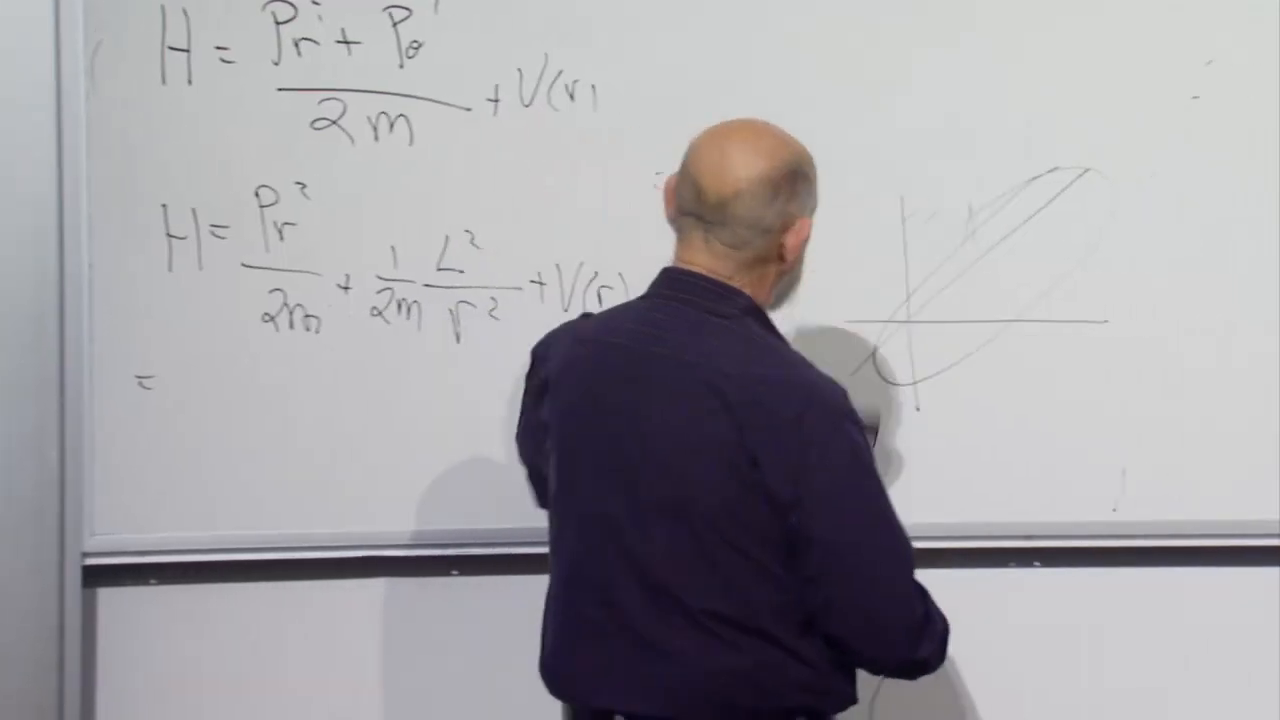
\includegraphics[width=0.9\linewidth]{lecture_03_frame_03.png}\caption{عند تثبيت \(\ell\)، تخضع الدالة الموجية الشعاعية المختزلة لمعادلة Schr\"odinger أحادية البعد مع حد طرد مركزي يتناسب مع \(\ell(\ell+1)/r^2\).}\lectureframe{00:54:32}\end{figure}

لقد اختُزل البنيان الزاوي الثلاثي الأبعاد في المعلمة \(\ell\). ولا يظهر العدد الكمي المغناطيسي \(m\) في المعادلة الشعاعية.

\begin{classroomqa}\lecturetimestamp{00:55:34}\audiencequestion{بالنسبة إلى \(\ell\) معيَّن، هل تمتلك الحالات المغناطيسية \(2\ell+1\) الطاقة نفسها؟}\lecturerresponse{نعم، شريطة تثبيت الحالة الذاتية الشعاعية أيضًا. فلكل \(u_{n_r\ell}\) مختار، تكون لجميع القيم \(m=-\ell,\ldots,\ell\) الطاقة نفسها لأن \(m\) لا يدخل في المعادلة الشعاعية. أما الحالات الذاتية الشعاعية المختلفة عند \(\ell\) نفسه فلها عمومًا طاقات مختلفة.}\end{classroomqa}

\begin{classroomqa}
\lecturetimestamp{00:56:03}
\audiencequestion{لماذا يمكن استبدال \(L^2\) بـ \(\hbar^2\ell(\ell+1)\)، وكيف ترتبط \(\ell\) بالقيم المسموح بها لـ \(m\)؟}
\lecturerresponse{العدد \(\ell\) يميّز متعددية العزم الزاوي، وهو أكبر قيمة فيها لـ \(m\). ولكل حالة في تلك المتعددية القيمة الذاتية نفسها لـ \(L^2\)، وهي \(\hbar^2\ell(\ell+1)\)، ولذلك تُدرج تلك القيمة الذاتية في المعادلة الشعاعية.}
\end{classroomqa}

لا نحتاج إلى الحلول الصريحة بالدوال الخاصة في الاستدلال الحالي. وما يهم هو كيفية تنظيم الحلول.

\section{العقد الشعاعية ومستويات الطاقة}

عند تثبيت \(\ell\)، تكون المعادلة الشعاعية المختزلة مسألة قيم ذاتية عادية أحادية البعد. وتُرتَّب حالاتها المقيدة بحسب عدد العقد الداخلية فيها. فأدنى حالة شعاعية لا تحتوي على أي عقدة داخلية، والتي تليها تحتوي على عقدة واحدة، والتي بعدها تحتوي على عقدتين. وتعني زيادة عدد العقد تغيرًا أسرع في الدالة الموجية؛ والتغير الأسرع يعني زخمًا أكبر، ومن ثم طاقة حركية أكبر.

يحدِّد كل مقدار من \(\ell\) مؤثرًا شعاعيًا مختلفًا لأن الحد النابذ المركزي يتغير مع \(\ell\). ومن ثم فإن \(\ell=0,1,2,\ldots\) تعطي سلاسل شعاعية منفصلة. ويزيح الحد النابذ المركزي الموجب المستويات إلى أعلى مع إضافة العزم الزاوي. وتحمل كل قيمة ذاتية شعاعية عند تثبيت \(\ell\) متعددية مغناطيسية بُعدها
\begin{equation}
2\ell+1.
\end{equation}
والمستويات ذات \(\ell=0\) أحادية، وذات \(\ell=1\) ثلاثية، وذات \(\ell=2\) خماسية. وهذه هي الانحلالات التي يضمنها التناظر الدوراني؛ وقد يجعل تناظر إضافي أيضًا الحالات ذات القيم المختلفة لـ \(\ell\) منحلةً كذلك.

بالنسبة إلى الكمونات من النوع الذري التي تحقق \(V(r)\to0\) عند القيم الكبيرة لـ \(r\)، تؤخذ عتبة الإفلات اصطلاحًا عند \(E=0\). وتشكل حالات الطاقة السالبة الطيف المنفصل المقيد. وعند \(E=0\) وما فوقه نصادف المتصل التشتتي. وتعتمد هذه العبارة على سلوك الكمون عند القيم الكبيرة لـ \(r\)، ولا تنطبق على كمون مركزي حابس.

\section{الانحلال الكولومي الخاص}

للکمون الكولومي الدقيق اللامنسبي اصطفاف إضافي للمستويات. فللحالة الشعاعية الدنيا ذات \(\ell=1\) الطاقة نفسها التي لأول حالة مثارة ذات \(\ell=0\). وتتراصف الحالة التالية ذات \(\ell=1\) مع ثاني حالة مثارة ذات \(\ell=0\)، وتنضم إليهما الحالة الدنيا ذات \(\ell=2\). ويستمر هذا النمط عبر السلاسل الأعلى شعاعيًا وزاويًا.

\begin{classroomqa}
\lecturetimestamp{01:09:57}
\audiencequestion{هل يشير هذا الانحلال الكولومي الإضافي إلى تناظر آخر؟}
\lecturerresponse{نعم. إنه تناظر إضافي غير مألوف للكمون الكولومي الدقيق. فالتغييرات الصغيرة في الكمون تفسد هذا الاصطفاف، ولا نتابع اشتقاقه هنا.}
\end{classroomqa}

وتكون انحلالات الأغلفة المدارية الناتجة
\begin{equation}
1,\qquad 4,\qquad 9,\qquad 16,\qquad \ldots
\end{equation}
قبل إدخال اللف المغزلي للإلكترون.

\begin{classroomqa}
\lecturetimestamp{01:11:46}
\audiencequestion{هل يصف هذا الانحلال الهيدروجين، أم يصف فقط مسألة كولوم المثالية؟}
\lecturerresponse{يحققه الهيدروجين تقريبًا جيدًا جدًا، ولكن ليس على نحو دقيق تمامًا. فالتصحيحات النسبية والحجم المنتهي للنواة يخلّان بالنمط الكولومي المثالي.}
\end{classroomqa}

تعطي النواة النقطية كمونًا دقيقًا من النمط \(1/r\). أما النواة التي تكون شحنتها موزعة على حجم صغير فتولد كمونًا مختلفًا قليلًا عندما ينفذ الإلكترون إلى ذلك الحجم، وحتى هذا الانحراف الصغير يزيل جزءًا من الانحلال الخاص.

وقد أُهمل اللف المغزلي أيضًا. إن إدخال حالتي اللف المغزلي للإلكترون يضاعف عدد الحالات في الأغلفة ليصبح
\begin{equation}
2,\qquad 8,\qquad 18,\qquad 32,\qquad \ldots
\end{equation}
قبل تمييز الانشقاقات الإضافية في معالجة ذرية أكثر اكتمالًا.

\section{إعادة النظر في المعادلة الديكارتية}

المعادلة التي بدأت منها المسألة الشعاعية هي معادلة Schr\"odinger ثلاثية الأبعاد المستقلة عن الزمن
\begin{equation}
\begin{aligned}
-\frac{\hbar^2}{2m}\nabla^2\Psi+V(r)\Psi&=E\Psi,\\
\nabla^2&=\frac{\partial^2}{\partial x^2}
+\frac{\partial^2}{\partial y^2}
+\frac{\partial^2}{\partial z^2},\\
r&=\sqrt{x^2+y^2+z^2}.
\end{aligned}
\end{equation}
ثم ننتقل إلى الإحداثيات الشعاعية والزاوية ونختار حالة ذاتية لـ \(L^2\). وعندئذ يؤدي استبدال \(L^2\) بـ \(\hbar^2\ell(\ell+1)\) إلى اختزال المعادلة التفاضلية الجزئية إلى المعادلة الشعاعية العادية أعلاه.

\begin{classroomqa}
\lecturetimestamp{01:16:42}
\audiencequestion{هل يمكن استخدام الانحرافات عن طيف كولوم المثالي لتحديد حجم النواة؟}
\lecturerresponse{ليس بهذه المقارنة البسيطة. فهناك تصحيحات أخرى أكبر بكثير، ويجب أخذها في الحسبان أولًا. ويُذكر حجم النواة هنا لأنه يعطي مثالًا مباشرًا على انحراف عن كمون كولوم النقطي.}
\end{classroomqa}

\begin{classroomqa}
\lecturetimestamp{01:17:09}
\audiencequestion{ما الفرق الرئيسي بين حدي العزم الزاوي الكلاسيكي والكمومي؟}
\lecturerresponse{كلاسيكيًا، يكون \(L^2\) هو المربع المعتاد لمقدار متجه محفوظ. أما في متعددية مدارية كمومية فقيمته الذاتية هي \(\hbar^2\ell(\ell+1)\)، لا ببساطة \(\hbar^2\ell^2\). ويأتي الحد الإضافي من عدم تبديل مركبات العزم الزاوي.}
\end{classroomqa}

\begin{classroomqa}
\lecturetimestamp{01:17:58}
\audiencequestion{هل للدوال الموجية للحالات المقيدة دعم متراص؟}
\lecturerresponse{لا. فهي تمتد إلى أي بُعد عن المركز. وبالنسبة إلى الحالات الذرية المقيدة قيد المناقشة، فإنها تتناقص أسيًا عند المسافات الكبيرة، بحيث يصبح الاحتمال مهمَلًا لكنه لا ينعدم خارج أي نصف قطر منتهٍ.}
\end{classroomqa}

\begin{classroomqa}
\lecturetimestamp{01:18:48}
\audiencequestion{عندما يُلغي \(\ell=0\) بئر الطرد المركزي، ماذا يحدث للنقطة المستقرة؟}
\lecturerresponse{لا يعود هناك حد أدنى ينشأ من التنافس بين الحاجز النابذ المركزي وقوة التجاذب. وفي تقريب كولوم النقطي، تتجه الحركة الكلاسيكية نحو المركز المفرد. وكموميًا لا يمكن لأدنى حالة أن تكون لها في آنٍ معًا موضع محدد تمامًا عند المركز وزخم صفري، ولذلك تكون للدالة الموجية الدنيا درجة انتشار مكاني منتهية.}
\end{classroomqa}

\editorialnote{بالنسبة إلى كمون مركزي منتظم، قد يستمر مسار كلاسيكي صفري العزم الزاوي عبر الأصل. أما في كمون كولوم النقطي المثالي، فإن \(r=0\) يكون بدلًا من ذلك تفردًا تصادميًا، ويتطلب استمرار المسار الكلاسيكي وصفة إضافية.}

أدى الاختزال الكلاسيكي إلى وضع مدار واحد في مستوى، لكن لا يمكن تطبيق تلك الخطوة على دالة موجية كمومية بالطريقة نفسها. فالحالة المدارية الكمومية تملأ الفضاء الثلاثي الأبعاد. والمؤثر الزاوي الكامل هو \(L^2=L_x^2+L_y^2+L_z^2\)، وتحتفظ قيمته الذاتية بالنتيجة الثلاثية الأبعاد \(\hbar^2\ell(\ell+1)\).

\begin{classroomqa}
\lecturetimestamp{01:21:30}
\audiencequestion{كيف يمكن أن تظل المسألة الكمومية ثلاثية الأبعاد بعد وضع المدار الكلاسيكي في مستوى؟}
\lecturerresponse{الذي وُضع في مستوى ثابت هو المدار الكلاسيكي وحده، وذلك باختيار إحداثيات متعامدة مع متجه عزمه الزاوي المحفوظ. أما الدالة الموجية الكمومية فتشغل الفضاء الثلاثي الأبعاد. وتبقى المركبات الأخرى للعزم الزاوي حاضرة عبر \(L^2\)، ولهذا تحتوي المعادلة الشعاعية على \(\ell(\ell+1)\) لا على مجرد مربع مركبة واحدة.}
\end{classroomqa}

\begin{classroomqa}
\lecturetimestamp{01:22:54}
\audiencequestion{هل تقبل كل مسألة كمومية مؤثرات رفع وخفض؟}
\lecturerresponse{لا. إنها تظهر في حالات مواتية على نحو غير معتاد. والعزم الزاوي إحدى هذه الحالات، والمذبذب التوافقي حالة أخرى. وحالة المذبذب مفيدة على نحو خاص لأن الحركة قرب اتزان مستقر تكون في كثير من الأحيان تقريبًا توافقية، بما في ذلك الاهتزازات الشعاعية الصغيرة قرب الحد الأدنى من كمون فعال.}
\end{classroomqa}

تُترك المسألة الذرية جانبًا عند هذه النقطة، ويصبح المذبذب التوافقي المثال التالي لطيف تحدده مؤثرات السلم.

\section{الاهتزازات الصغيرة والمذبذب التوافقي}

قرب اتزان مستقر، تؤدي إزاحة صغيرة بما يكفي في كثير من الأحيان إلى حركة توافقية. ويوفر الكمون الشعاعي الفعال عند عزم زاوي غير صفري مثالًا على ذلك: فالحركة الشعاعية القريبة من قاع بئره تكون تقريبًا توافقية.

اعتبر مذبذبًا أحادي البعد كتلته واحد. لتكن \(x\) الإزاحة عن موضع الاتزان، واكتب ثابت النابض على الصورة \(k=\omega^2\). يكون الهاملتوني الكلاسيكي
\begin{equation}
H=\frac{p^2}{2}+\frac{\omega^2x^2}{2}.
\end{equation}
وتعطي معادلات هاملتون
\begin{equation}
\dot{x}=\frac{\partial H}{\partial p}=p,
\qquad
\dot{p}=-\frac{\partial H}{\partial x}=-\omega^2x,
\end{equation}
ومن ثم
\begin{equation}
\ddot{x}=-\omega^2x.
\end{equation}
وهكذا يكون \(\omega\) هو التردد الكلاسيكي للاهتزاز.

\section{التحليل إلى عوامل وطاقة نقطة الصفر}

كموميًا،
\begin{equation}
[x,p]=i\hbar.
\end{equation}
والهاملتوني هو مجموع مربعات، مما يقترح التحليل إلى العوامل
\begin{align}
\frac{1}{2}(p+i\omega x)(p-i\omega x)
&=\frac{1}{2}\left(p^2+\omega^2x^2+i\omega[x,p]\right) \\
&=\frac{1}{2}\left(p^2+\omega^2x^2-\hbar\omega\right).
\end{align}
ومن ثم
\begin{equation}
H=\frac{1}{2}(p+i\omega x)(p-i\omega x)
+\frac{1}{2}\hbar\omega.
\end{equation}
والحد الإضافي \(\hbar\omega/2\) هو طاقة نقطة الصفر.

كلاسيكيًا، كانت أدنى طاقة ستقع عند \(x=p=0\). أما كموميًا، فلا يمكن لأي حالة أن يكون فيها كل من الموضع والزخم مثبتين بدقة عند الصفر. وفوق ذلك فإن الحدين \(p^2/2\) و\(\omega^2x^2/2\) موجبان ولا يمكن أن يلغي أحدهما الآخر. ولذلك لا مفر من طاقة غير صفرية للحالة الأرضية.

في حساب مؤثرات السلم، يمكن تنحية الثابت الإضافي المشترك مؤقتًا ثم إعادته في النهاية.

\begin{classroomqa}
\lecturetimestamp{01:36:10}
\audiencequestion{هل تخبرنا الإشارة الموجبة لحد طاقة نقطة الصفر بشيء إضافي؟}
\lecturerresponse{هاملتوني المذبذب مؤثر موجب: فهو مجموع مربعات موجبة، ومن ثم لا يمكن أن تكون طاقته سالبة.}
\end{classroomqa}

\section{سلم المذبذب}

نُدخِل المؤثرين عديمي البعد\footnote{عند \(01{:}37\)--\(01{:}42\) تقريبًا، يستخدم الحساب \(\hbar=1\). ويُعاد إدخال العامل \(\hbar\) في هذه التعريفات المطبَّعة بحيث يكون \(A_\pm\) عديمي البعد وتكون مبدلتهما مساوية للواحد.}
\begin{equation}
A_+=\frac{p+i\omega x}{\sqrt{2\hbar\omega}},
\qquad
A_-=\frac{p-i\omega x}{\sqrt{2\hbar\omega}}.
\end{equation}
وهما مترافقان هيرميتيًا:
\begin{equation}
A_+^\dagger=A_-.
\end{equation}
ومبدلتهما هي
\begin{align}
[A_-,A_+]
&=\frac{1}{2\hbar\omega}
\left([p,i\omega x]+[-i\omega x,p]\right) \\
&=1.
\end{align}

نعرّف
\begin{equation}
N=A_+A_-.
\end{equation}
وعندئذٍ يكون الهاملتوني
\begin{equation}
H=\hbar\omega\left(N+\frac{1}{2}\right).
\end{equation}
ومن ثم يختزل إيجاد طيف الطاقة إلى إيجاد القيم الذاتية لـ \(N\).

لنفترض
\begin{equation}
N|n\rangle=n|n\rangle.
\end{equation}
المبدلات مع \(N\) هي\footnote{تُستعاد الخطوات الوسيطة عند \(01{:}45{:}37\)--\(01{:}48{:}10\) مباشرةً من العلاقات المعطاة \(N=A_+A_-\) و\([A_-,A_+]=1\).}
\begin{align}
[N,A_+]
&=A_+[A_-,A_+]=A_+, \\
[N,A_-]
&=[A_+,A_-]A_-=-A_-.
\end{align}
ويترتب على ذلك أن
\begin{align}
N\bigl(A_+|n\rangle\bigr)
&=(n+1)A_+|n\rangle, \\
N\bigl(A_-|n\rangle\bigr)
&=(n-1)A_-|n\rangle.
\end{align}
ومن ثم فإن \(A_+\) يرفع قيمةً ذاتيةً لـ \(N\) بمقدار واحد، و\(A_-\) يخفضها بمقدار واحد متى كان المتجه الناتج غير صفري.

المؤثر \(N\) غير سالب:
\begin{equation}
\langle\psi|N|\psi\rangle
=\langle\psi|A_+A_-|\psi\rangle
=\|A_-|\psi\rangle\|^2
\geq0.
\end{equation}
ولذلك لا يمكن لعملية الخفض أن تستمر إلى قيم ذاتية سالبة. وعند حالة دنيا \(|b\rangle\)، لا بد أن تتوقف:
\begin{equation}
A_-|b\rangle=0.
\end{equation}

بالنسبة إلى الحالات الذاتية المطبَّعة، تتحدد معاملات السلم من معاييرها:
\begin{align}
\|A_-|n\rangle\|^2
&=\langle n|A_+A_-|n\rangle=n, \\
\|A_+|n\rangle\|^2
&=\langle n|A_-A_+|n\rangle=n+1.
\end{align}
ولذلك يمكن اختيار الأطوار بحيث
\begin{equation}
A_-|n\rangle=\sqrt{n}\,|n-1\rangle,
\qquad
A_+|n\rangle=\sqrt{n+1}\,|n+1\rangle.
\end{equation}

\begin{classroomqa}
\lecturetimestamp{01:52:42}
\audiencequestion{إذا كان \(A_-\) يخفض حالةً وكان \(A_+\) يرفعها من جديد، فكيف يُنتج \(A_+A_-\) القيمة الذاتية \(n\)؟}
\lecturerresponse{يتضمن فعل السلم عواملَ تطبيع. فالفعل أولًا بـ \(A_-\) يعطي \(\sqrt n\)، والفعل بـ \(A_+\) على الحالة الناتجة يعطي \(\sqrt n\) أخرى. وحاصل ضربهما هو \(n\).}
\end{classroomqa}

وبالفعل،
\begin{equation}
A_+A_-|n\rangle
=\sqrt n\,A_+|n-1\rangle
=n|n\rangle.
\end{equation}

\begin{classroomqa}
\lecturetimestamp{01:55:52}
\audiencequestion{هل يجب أن تكون أدنى قيمة ذاتية لـ \(N\) صفراً، أم يمكن أن تكون موجبة؟}
\lecturerresponse{لا بد أن تكون صفراً، ويتألف طيف \(N\) من الأعداد الصحيحة غير السالبة. ولم يُقدَّم بعدُ برهان على هذه النهاية.}
\end{classroomqa}

\editorialnote{لتكن \(|b\rangle\) حالةً دنيا. وبما أن الخفض لا بد أن ينتهي، فإن \(A_-|b\rangle=0\). ويترتب على ذلك فورًا أن \(N|b\rangle=A_+A_-|b\rangle=0\)، ومن ثم فإن أدنى قيمة ذاتية لـ \(N\) هي الصفر.}

بالانطلاق من هذه الحالة الدنيا وتطبيق \(A_+\) نحصل على
\begin{equation}
n=0,1,2,\ldots.
\end{equation}
ومع إعادة الحد الجمعي لطاقة نقطة الصفر، تكون طاقات المذبذب
\begin{equation}
E_n=\hbar\omega\left(n+\frac{1}{2}\right),
\qquad n=0,1,2,\ldots.
\end{equation}

سيُطوَّر جبر المذبذب أكثر ويُستخدم لحل مسائل كمومية أخرى.
\chapter{دوال الموجة للمذبذب، واللفّ المغزلي نصفي، وتبادل الجسيمات}

\section{المذبذبات في كل مكان}

يمكن لأي نظام له اتزان مستقر أن يتذبذب عندما يُزاح عن ذلك الاتزان. وقد يكون له تردد واحد أو عدة ترددات. فوتر الكمان، على سبيل المثال، له نمط أساسي وتوافقيات أعلى. ونقره يثير تركيبًا ما من تلك الأنماط.

غير أن الأمثلة الأهم هنا هي الحقول. فتهيئة الاتزان للحقل الكهرومغناطيسي هي الفراغ: لا مجال كهربائي، ولا مجال مغناطيسي، ولا تذبذب كهرومغناطيسي. وإذا أُدخل إشعاع إلى تجويف أو إلى دليل موجي، أمكن للحقل أن يتذبذب في أنماطه المسموح بها، ولكل منها ترددها الخاص. وفي النظرية الكمية تصف تلك الأنماط مجموعات من الفوتونات.

وتنطبق الفكرة نفسها على البلورة. ومن المضلل أن نتصور كل ذرة على أنها مذبذب مستقل. فالذرات تؤثر بعضها في بعض بقوى، لذا فإن إزاحة ذرة واحدة تؤثر في جاراتها وتنتقل موجة عبر البلورة. والأنماط العادية لتلك الحركة المقترنة هي مذبذبات توافقية، وتسمى كمّاتها فونونات. والفوتونات والفونونات أشياء فيزيائية مختلفة، لكن كليهما يعيدنا إلى جبر المذبذب نفسه.

\section{جبر المذبذب}

في مناقشة المذبذب، نأخذ الكتلة وثابت بلانك المختزل مساويين للواحد:
\[
m=1,\qquad \hbar=1.
\]
ويكون الهاملتوني
\begin{equation}
H=\frac{p^{2}}{2}+\frac{\omega^{2}x^{2}}{2}.
\end{equation}
ويحدد المعامل \(\omega\) انحناء الجهد، وهو أيضًا تردد التذبذب.

عرّف مؤثري الرفع والخفض بـ
\begin{equation}
A_{\pm}=\frac{p\pm i\omega x}{\sqrt{2\omega}}.
\end{equation}
واختير عامل التطبيع بحيث
\begin{equation}
[A_{-},A_{+}]=1.
\end{equation}
ومؤثر العدد هو
\begin{equation}
N=A_{+}A_{-}.
\end{equation}
ومعًا، تفيد هذه المعادلات أن \(A_{+}\) يرفع قيمة ذاتية لـ \(N\) بمقدار واحد، وأن \(A_{-}\) يخفضها بمقدار واحد. والطيف الناتج هو
\begin{equation}
n=0,1,2,3,\ldots .
\end{equation}

كما أن ضرب مؤثري السُّلَّم أحدهما في الآخر يكشف التصحيح الكمي للطاقة الكلاسيكية:
\begin{align}
N
&=\frac{1}{2\omega}(p+i\omega x)(p-i\omega x)\\
&=\frac{1}{2\omega}\left(p^{2}+\omega^{2}x^{2}
 +i\omega[x,p]\right)\\
&=\frac{1}{2\omega}\left(p^{2}+\omega^{2}x^{2}-\omega\right),
\end{align}
حيث \([x,p]=i\). وبالتالي،
\begin{equation}
H=\omega\left(N+\frac12\right).
\end{equation}
وإذا كان الثابت الإضافي غير ذي صلة بالمسألة، فمن الملائم استعمال الهاملتوني المزاح
\begin{equation}
H_{\mathrm{shifted}}=H-\frac{\omega}{2}=\omega N.
\end{equation}
والحد \(\omega/2\) هو طاقة النقطة الصفرية، أو طاقة الحالة الأرضية، للمذبذب. وبالنسبة إلى نمط حقلي، يسمى الحد المناظر طاقة الفراغ. وهو يعكس مبدأ عدم اليقين: فلا يمكن لأي حالة أن يكون فيها كل من \(x\) و\(p\) مساويًا للصفر على نحو حاد، ولذلك لا يمكن أن تكون للحدين التربيعيين الموجبين في \(H\) قيمة توقعية صفرية معًا.

\begin{classroomqa}
\lecturetimestamp{00:09:46}
\audiencequestion{لماذا يشتمل طيف مؤثر العدد على الصفر؟}
\lecturerresponse{يمكن البرهنة على ذلك صراحةً ببناء الدالة الموجية للحالة الأرضية. وسيُظهر هذا البناء حالةً لها \(N=0\).}
\end{classroomqa}

ولبدء هذا البناء، استبدل متجهات الحالة بدوال موجية للموضع. فتصبح حالات الطاقة الذاتية
\[
\psi_{0}(x),\ \psi_{1}(x),\ \psi_{2}(x),\ldots,
\]
وتؤثر المؤثرات الأساسية على النحو
\begin{equation}
X\longmapsto x,\qquad
P\longmapsto -i\frac{d}{dx}.
\end{equation}
ومع إعادة \(\hbar\)، يصبح الاستبدال الثاني
\(P\mapsto-i\hbar\,d/dx\).

قبل حل \(\psi_{0}\)، توجد إجابة تجريدية أسرع عن السؤال. فعلى سُلَّم حالات القيم الذاتية المنفصل والقابلة للتطبيع للمذبذب، يكون \(N=A_{+}A_{-}\) غير سالب، لذا لا يمكن أن يستمر الخفض المتكرر بخطوات وحدوية إلى ما لا نهاية. وعند الطرف النهائي---الذي ستُبنى دالته الموجية القابلة للتطبيع أدناه---لا بد من وجود حالة، نرمز لها بـ \(\lvert0\rangle\)، بحيث
\begin{equation}
A_{-}\lvert0\rangle=\mathbf 0.
\end{equation}
وإلا لكان \(A_{-}\lvert0\rangle\) حالةً أخرى أخفض بدرجة واحدة. ويترتب على ذلك فورًا أن
\begin{equation}
N\lvert0\rangle
=A_{+}A_{-}\lvert0\rangle
=\mathbf 0
=0\,\lvert0\rangle.
\end{equation}
ومن ثم فإن القيمة الذاتية لمؤثر العدد في الحالة الدنيا هي الصفر.

\begin{classroomqa}
\lecturetimestamp{00:14:57}
\audiencequestion{إذا كانت القيمة الذاتية هي الصفر، أفلا ينبغي أن يحتوي الطرف الأيمن على متجه ذاتي صفري؟}
\lecturerresponse{الكت \(\lvert0\rangle\) متجه مطبَّع غير صفري ووسمه صفر. وفي \(N\lvert0\rangle=0\,\lvert0\rangle\) يكون الطرف الأيمن هو المتجه الصفري. وكت الحالة الأرضية والمتجه الصفري شيئان مختلفان.}
\end{classroomqa}

\section{معادلة Schr\"odinger والحلول الفيزيائية}

لنعد الآن إلى تمثيل الموضع. معادلة Schr\"odinger غير المعتمدة على الزمن هي
\begin{equation}
\left[
-\frac12\frac{d^{2}}{dx^{2}}
+\frac12\omega^{2}x^{2}
\right]\psi(x)=E\psi(x).
\end{equation}
وبوصفها معادلة تفاضلية من الرتبة الثانية، فلها حلول صورية لقيم اعتباطية لـ \(E\). وليست معظم تلك الحلول الصورية حالات فيزيائية للمذبذب. إذ إنها تنمو أسيًا عند القيم الكبيرة لـ \(\lvert x\rvert\)، ولذلك يتباعد معيارها.

في الحالة المقيدة، يجب أن تكون الدالة الموجية قابلة للتكامل تربيعيًا:
\begin{equation}
\int_{-\infty}^{\infty}\psi^{*}(x)\psi(x)\,dx<\infty.
\end{equation}
وعندئذ يمكن تطبيعها بحيث يساوي التكامل واحدًا. ولا تنتج مثل هذه الحلول إلا عن قيم خاصة للطاقة. وحالات الموضع والزخم على مستقيم لا نهائي استثنائية من هذه الناحية، لكن حلول المذبذب التي تنمو أسيًا تُستبعد ببساطة من فضاء الحالات.

\section{الحالة الأرضية الغاوسية}

يمكن حل معادلة الرتبة الثانية، لكن جبر السُّلَّم يعطينا معادلة أبسط من الرتبة الأولى:
\begin{equation}
A_{-}\psi_{0}(x)=0.
\end{equation}
والعامل الكلي في \(A_{-}\) غير مؤثر عندما يكون الطرف الأيمن صفرًا، ولذلك يكافئ هذا
\begin{equation}
(p-i\omega x)\psi_{0}(x)=0.
\end{equation}
وباستخدام \(p=-i\,d/dx\) نحصل على
\begin{equation}
\left(\frac{d}{dx}+\omega x\right)\psi_{0}(x)=0.
\end{equation}

\begin{classroomqa}
\lecturetimestamp{00:22:32}
\audiencequestion{هل يمكن حل هذا بفصل المتغيرات؟}
\lecturerresponse{ليس هناك إلا متغير مستقل واحد، لذلك لا يوجد متغيران لفصلهما. وعند كتابة المعادلة على الصورة \(\psi_{0}'/\psi_{0}=-\omega x\)، تكون على هيئة مشتقة لوغاريتمية. وهذا يقترح كتابة الدالة الموجية على هيئة أسية.}
\end{classroomqa}

ومن الطرق المفيدة لحلها أن نكتب
\begin{equation}
\psi_{0}(x)=e^{f(x)}.
\end{equation}
وعندئذ
\[
\psi_{0}'(x)=f'(x)e^{f(x)},
\]
ويلغى العامل الأسي المشترك. وتختزل المعادلة إلى
\begin{equation}
\frac{df}{dx}+\omega x=0.
\end{equation}

\begin{classroomqa}
\lecturetimestamp{00:26:28}
\audiencequestion{هل ينبغي أن تظهر إشارة سالب في \(f(x)\)؟}
\lecturerresponse{نعم. بما أن \(df/dx=-\omega x\)، فإن التكامل يعطي حدًا تربيعيًا سالبًا.}
\end{classroomqa}

إذن
\begin{equation}
f(x)=-\frac12\omega x^{2}+C,
\end{equation}
و
\begin{equation}
\psi_{0}(x)\propto e^{-\omega x^{2}/2}.
\end{equation}
ويُترك ثابت التطبيع الضربي دون تحديد. والنقطة المهمة هي الشكل الغاوسي: فهو أملس، ومتمركز قرب الأصل، ويتناقص سريعًا عند القيم الكبيرة لـ \(\lvert x\rvert\). ومن الواضح أنه قابل للتكامل تربيعيًا.

لا حاجة إلى إعادة التعويض بالحل في معادلة الرتبة الثانية لاستخراج طاقته. فالجبر يعطينا بالفعل
\begin{equation}
E_{0}=\frac{\omega}{2}.
\end{equation}

\section{الحالات المثارة، والعقد، والحركة الكلاسيكية}

تنتج الحالة المثارة الأولى من رفع الحالة الأرضية:
\begin{equation}
\psi_{1}(x)\propto A_{+}\psi_{0}(x)
\propto(p+i\omega x)e^{-\omega x^{2}/2}.
\end{equation}
ومعادلة الحالة الأرضية تقول
\[
p\psi_{0}=i\omega x\,\psi_{0}.
\]
إن تغيير الإشارة في مؤثر السُّلَّم يحول الإلغاء إلى جمع:
\begin{equation}
(p+i\omega x)\psi_{0}
=2i\omega x\,\psi_{0}.
\end{equation}
وباستثناء ثابت كلي،
\begin{equation}
\psi_{1}(x)\propto x\,e^{-\omega x^{2}/2}.
\end{equation}

هذه الدالة الموجية فردية:
\begin{equation}
\psi_{1}(-x)=-\psi_{1}(x).
\end{equation}
وكثافة احتمالها زوجية، لكنها تحتوي على عقدة عند الأصل،
\begin{equation}
\lvert\psi_{1}(0)\rvert^{2}=0.
\end{equation}
ومن ثم فإن كثافة احتمال الحالة المثارة الأولى لها عقدة عند \(x=0\).

ويؤدي التأثير المتكرر لـ \(A_{+}\) إلى كثيرات حدود أعلى درجة تضرب الغلاف الغاوسي نفسه.\footnote{تذكر المحاضرة عوامل كثيرات الحدود الأعلى درجة، والعقدة الإضافية عند كل خطوة، والتناظر المتناوب من \(00{:}34{:}25\) إلى \(00{:}35{:}49\). ويؤكد Leonard Susskind وArt Friedman هذه الصيغة، أي غاوسي مضروبًا في كثيرة حدود، في \emph{Quantum Mechanics: The Theoretical Minimum} (2014)، في مناقشتهما للدوال الذاتية للمذبذب.} وحتى التطبيع،
\begin{equation}
\psi_{n}(x)=P_{n}(x)e^{-\omega x^{2}/2}.
\end{equation}
ويتناوب التكافؤ بين الزوجية والفردية، وتضيف كل خطوة عقدة. ومع ازدياد \(n\)، تمتد الدالة الموجية أبعد عن الأصل وتطوّر تذبذبات أسرع.

ولهاتين السمتين معنيان فيزيائيان مباشران. فامتداد الدالة إلى ما هو أبعد عن الأصل يقابل طاقة وضع أكبر لأن الجهد ينمو مثل \(x^{2}\). والتذبذب السريع في فضاء الموضع يدل على زخم أكبر. ومن المرجح أن يبلغ مذبذب عالي الإثارة مسافات أبعد عن المركز؛ وعندما يمر عبر المنطقة المركزية يحمل زخمًا أكبر وتتذبذب دالته الموجية هناك بسرعة أكبر.

\begin{classroomqa}
\lecturetimestamp{00:37:18}
\audiencequestion{هل يفشل المذبذب التوافقي في الاقتراب من السلوك الكلاسيكي عندما يصبح \(n\) كبيرًا؟}
\lecturerresponse{لا تُمثَّل الحركة الكلاسيكية بحالة ذاتية ثابتة واحدة للطاقة. بل تظهر في حزمة موجية تضم مستويات طاقة كثيرة. فغاوسي مزاح، على سبيل المثال، يتطور ذهابًا وإيابًا مثل مذبذب كلاسيكي، ويصغر عدم اليقين النسبي كلما كبر مدى التأرجح.}
\end{classroomqa}

ابدأ بالغاوسي الخاص بالحالة الأرضية وأزحه عن الأصل. فالحزمة المزاحة لم تعد حالة ذاتية للطاقة؛ بل هي تراكب من عدد كبير من تلك الحالات. وتحت معادلة Schr\"odinger المعتمدة على الزمن، تكتسب مركباتها أطوارًا مختلفة. وتتأرجح الحزمة من أحد جانبي الجهد إلى الآخر، مطوِّرةً تغيرًا طوريًا سريعًا قرب المركز، ثم تعود فتصبح ملساء قرب نقطة انقلاب. وكلما كانت سعة التأرجح أكبر مقارنة بعرض الحزمة، بدت الحركة أقرب إلى الكلاسيكية.

\begin{classroomqa}
\lecturetimestamp{00:39:29}
\audiencequestion{هل ينبغي أن تمر الدالة الموجية للحالة المثارة الثانية عبر الصفر عند الأصل؟}
\lecturerresponse{لا. فعامل كثيرة الحدود فيها ليس مجرد \(x^{2}\)؛ بل يحتوي أيضًا على حد ثابت، ولذلك لا يلزم أن تنعدم الدالة الموجية عند \(x=0\).}
\end{classroomqa}

وتفترض حجة السلم أيضًا أن \(A_{+}\) و\(A_{-}\) مترافقان هيرميتيًا على مجال المذبذب المؤلف من الدوال القابلة للتكامل تربيعيًا، مع السلوك الحدّي اللازم لعلاقة المرافق. والحلول الصورية التي تنمو أسيًا لا تنتمي إلى ذلك المجال.

\begin{classroomqa}
\lecturetimestamp{00:40:45}
\audiencequestion{هل توجد طريقة عامة للتعرّف على الحالات التي يمكن فيها حل هاميلتوني بهذه الطرائق الجبرية؟}
\lecturerresponse{لا توجد قاعدة عامة من هذا النوع. والأمثلة القابلة للحل على نحو تام نادرة. فالمذبذب التوافقي وذرة الهيدروجين المثالية غير النسبية حالتان محظوظتان تنجح فيهما الطرائق الجبرية.}
\end{classroomqa}

\section{اللفّ المغزلي نصفيّ بوصفه زخمًا زاويًا}

اللفّ المغزلي هو زخم زاوي تحمله الجسيمة مستقلًا عن حركتها المدارية لمركز كتلتها. فالجسيمة الساكنة لا يكون لها زخم زاوي مداري \(\mathbf R\times\mathbf P\)، ولكن قد يكون لها مع ذلك لفّ مغزلي. ويمكن للمرء أن يحاول تصوّره على أنه جسم صغير يدور، أو أن يعامل اللفّ المغزلي بوصفه خاصية كمومية جوهرية. والعبارة الحاسمة رياضية: فمركّباته تتحول تحت الدورانات المكانية وتخضع لعلاقات الإبدال للزخم الزاوي.

أعِد \(\hbar\) من هذه النقطة فصاعدًا. تحقق مركّبات الزخم الزاوي
\begin{equation}
[L_{z},L_{x}]=i\hbar L_{y},
\end{equation}
وتُستحصل العلاقتان الأخريان بالتبديل الدوري. ومصفوفات باولي عديمة الأبعاد هي
\begin{equation}
\begin{aligned}
\sigma_{z}&=
\begin{pmatrix}
1&0\\
0&-1
\end{pmatrix},\\[0.4em]
\sigma_{x}&=
\begin{pmatrix}
0&1\\
1&0
\end{pmatrix},\\[0.4em]
\sigma_{y}&=
\begin{pmatrix}
0&-i\\
i&0
\end{pmatrix}.
\end{aligned}
\end{equation}
وفي هذا الأساس تكون \(\sigma_{z}\) قطرية. وقيمها الذاتية هي \(+1\) و
\(-1\).

\begin{classroomqa}
\lecturetimestamp{00:47:35}
\audiencequestion{هل توجد إشارة سالبة في \(\sigma_x\)؟}
\lecturerresponse{لا. فالعنصران خارج القطر في \(\sigma_x\) كلاهما موجب.}
\end{classroomqa}

يبدأ الحساب على اللوح عند \(00{:}49{:}35\) بعملية الضرب عنصرًا بعنصر. وبإتمام عمليات الضرب نحصل على
\begin{align}
\sigma_{z}\sigma_{x}
&=
\begin{pmatrix}
0&1\\
-1&0
\end{pmatrix}
=i\sigma_{y},\\
\sigma_{x}\sigma_{z}
&=
\begin{pmatrix}
0&-1\\
1&0
\end{pmatrix}
=-i\sigma_{y}.
\end{align}
ومن ثم
\begin{equation}
[\sigma_{z},\sigma_{x}]=2i\sigma_{y}.
\end{equation}
ومن ثم يُزال عامل الاثنين الزائد بتعريف مؤثرات اللفّ المغزلي الفيزيائية على الصورة التالية\footnote{يهمل الحساب على اللوح \(\hbar\). وقد أُعيد إدخاله هنا لكي تكون لـ \(S_i\) وحدات الزخم الزاوي.}
\begin{equation}
S_{i}=\frac{\hbar}{2}\sigma_{i}.
\end{equation}
وعندئذ
\begin{equation}
[S_{z},S_{x}]=i\hbar S_{y},
\end{equation}
وبالمثل بالنسبة إلى التبديلات الدورية. ومن ثم فإن أنصاف مصفوفات باولي، بعد إعادة عامل \(\hbar\)، تشكّل منظومة زخم زاوي.

بوضع \(\hbar=1\) نحصل على الصورة المبينة أدناه.\footnote{إطار المصدر هو \texttt{lecture\_04\_frame\_02.png}.}
\begin{figure}[htbp]
\centering
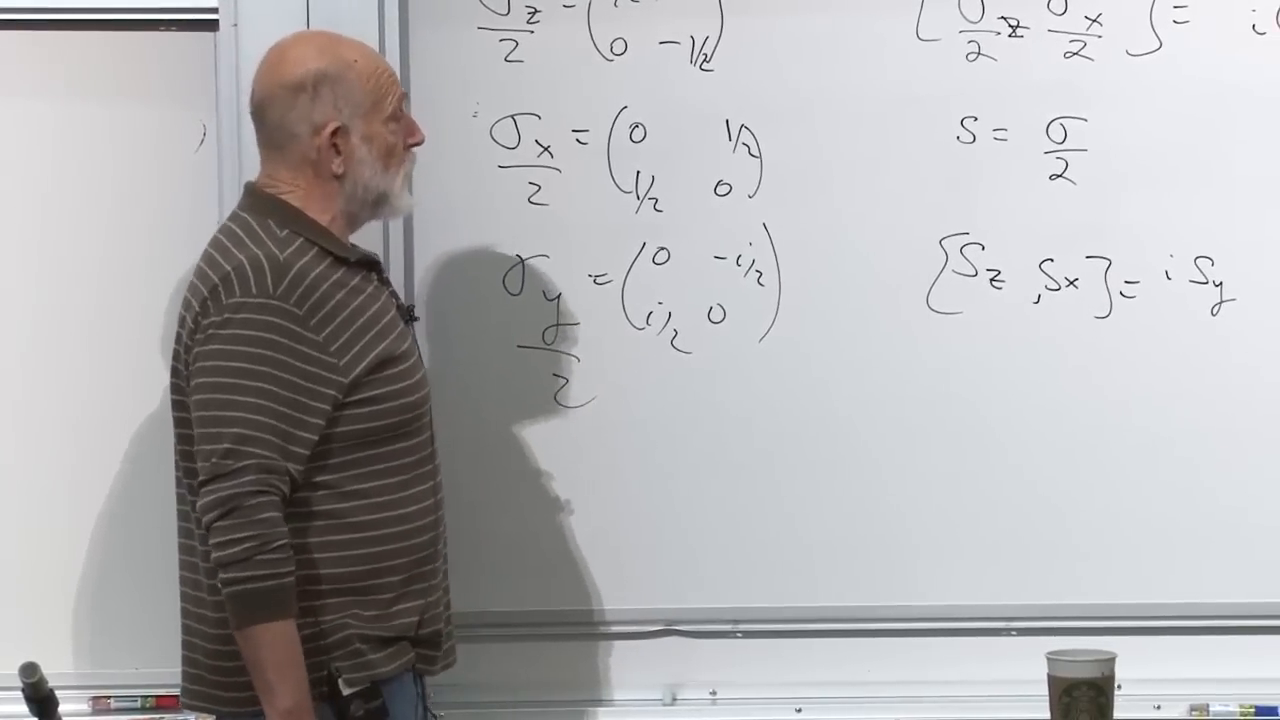
\includegraphics[width=0.9\linewidth]{lecture_04_frame_02.png}
\caption{في وحدات يكون فيها \(\hbar=1\)، تكون أنصاف مصفوفات باولي مؤثرات الزخم الزاوي للّفّ المغزلي نصفيّ وتحقق \([S_z,S_x]=iS_y\).}
\lectureframe{00:55:41}
\end{figure}

معادلتا القيم الذاتية لـ \(S_z\) هما
\begin{equation}
S_z\lvert\pm\rangle
=\pm\frac{\hbar}{2}\lvert\pm\rangle.
\end{equation}
وبصورة مكافئة، يكون عدد الكم المغناطيسي عديم الأبعاد
\begin{equation}
m_{s}=\pm\frac12,
\qquad
S_{z}\lvert m_{s}\rangle
=m_{s}\hbar\,\lvert m_{s}\rangle.
\end{equation}
وتغيّر مؤثرات الرفع والخفض للزخم الزاوي قيمة \(m\) بمقادير صحيحة، لكن هذا لا يقتضي أن يمر كل سلم عبر الصفر. فالمتعددات الصحيحة تضم قيمًا صحيحة لـ \(m\)، في حين تضم المتعددات نصف الصحيحة قيمًا نصف صحيحة. وبالنسبة إلى اللفّ المغزلي نصفيّ، لا يضم السلم إلا العضوين \(m_s=+1/2\) و\(m_s=-1/2\).

تشكل هاتان الحالتان ثنائية اللفّ المغزلي نصفيّ. ومن بين الجسيمات التي توصف بمثل هذه المتعددات ذات اللفّ المغزلي نصف الصحيح الإلكترونات والميونات والنيوترينوات والكواركات.

\section{الزخم الزاوي المداري واللفّ المغزلي}

لدينا الآن نوعان من الزخم الزاوي. فالزخم الزاوي المداري يصف الحركة بالنسبة إلى مبدأ إحداثي،
\begin{equation}
\mathbf L=\mathbf R\times\mathbf P,
\end{equation}
في حين أن \(\mathbf S\) هو اللفّ المغزلي الجوهري. ومجموعهما المتجهي هو الزخم الزاوي الكلي،
\begin{equation}
\mathbf J=\mathbf L+\mathbf S.
\end{equation}

\begin{classroomqa}
\lecturetimestamp{00:56:49}
\audiencequestion{إذا كان للنظام زخم زاوي كلي \(\mathbf J\)، فكيف يُحدَّد لفّه المغزلي \(\mathbf S\)؟}
\lecturerresponse{يُعطى عدد الكم المغزلي وعدد الكم المداري عادةً كلٌّ منهما على حدة. فإذا كان \(L=0\)، كان الزخم الزاوي كله لفًّا مغزليًا. وإلا لزمت القواعد الكمومية لجمع الزخوم الزاوية، وهي مؤجَّلة هنا.}
\end{classroomqa}

تنطبق قواعد الجمع على الزخم الزاوي المداري مضافًا إلى اللفّ المغزلي، وعلى لفّين مغزليين، أو على زخمين زاويين مداريين. وللنظام المركب قيمه المسموح بها الخاصة للزخم الزاوي الكلي، لكننا لا نحتاج إلى تلك القواعد بعد.

\begin{classroomqa}
\lecturetimestamp{00:58:18}
\audiencequestion{ما الدليل التجريبي الذي أدى إلى إدخال اللفّ المغزلي؟}
\lecturerresponse{قدّم التحليل الطيفي دليلًا، لكن الجدول الدوري يوفّر دافعًا واضحًا على نحو خاص: فبنيته القشرية تقتضي أن تمتلك الإلكترونات خاصية إضافية ثنائية القيم.}
\end{classroomqa}

\section{الانحلال الشبيه بالهيدروجين وعدّ الأغلفة}

بالنسبة إلى الزخم الزاوي المداري، فإن معادلة القيمة الذاتية لـ \(L^{2}\) هي
\begin{equation}
L^{2}\lvert\ell,m\rangle
=\hbar^{2}\ell(\ell+1)\lvert\ell,m\rangle,
\end{equation}
ولقيمة ثابتة من \(\ell\) يوجد
\begin{equation}
2\ell+1
\end{equation}
من الحالات المغناطيسية، الموافقة لـ \(m=-\ell,-\ell+1,\ldots,\ell\).

لمسألة كولوم المثالية غير النسبية انحلال إضافي. وطاقات حالاتها المقيدة سالبة وتقترب من الصفر من الأسفل، ولكن الذي يهم في العد هو تحاذي المستويات فحسب. فالمستوى الأول \(\ell=1\) يتحاذى مع المستوى التالي \(\ell=0\)؛ ويلتحق المستوى الأول \(\ell=2\) بالغلاف الرئيسي التالي؛ ويستمر النمط على هذا المنوال.\footnote{\texttt{lecture\_04\_frame\_03.png}، عند \(01{:}02{:}01\)؛ ويُذكر التحاذي الكامل للأغلفة الرئيسية من \(01{:}02{:}33\) إلى \(01{:}04{:}10\).}

\begin{figure}[htbp]
\centering
\begin{tikzpicture}[x=1.55cm,y=1.0cm]
\draw[->] (-0.65,0) -- (-0.65,4.35);
\draw[->] (-0.85,0) -- (4.75,0);
\node at (-0.95,4.08) {\(E\)};
\node at (4.55,-0.28) {\(\ell\)};
\node at (0,-0.30) {\(0\)};
\node at (2,-0.30) {\(1\)};
\node at (4,-0.30) {\(2\)};

\draw (-0.20,0.75) -- (0.20,0.75);

\draw (-0.20,2.00) -- (0.20,2.00);
\foreach \dx in {-0.18,0,0.18}
  \draw (2+\dx-0.06,2.00) -- (2+\dx+0.06,2.00);

\draw (-0.20,3.15) -- (0.20,3.15);
\foreach \dx in {-0.18,0,0.18}
  \draw (2+\dx-0.06,3.15) -- (2+\dx+0.06,3.15);
\foreach \dx in {-0.32,-0.16,0,0.16,0.32}
  \draw (4+\dx-0.05,3.15) -- (4+\dx+0.05,3.15);

\node[anchor=west] at (0.35,0.75) {\(n=1\)};
\node[anchor=west] at (2.35,2.00) {\(n=2\)};
\node[anchor=west] at (4.40,3.15) {\(n=3\)};
\end{tikzpicture}
\caption{تجمع الأغلفة الكولومية المثالية الثلاثة الأولى متعددات مدارية ذات الطاقة الرئيسية نفسها: حالة واحدة في الغلاف الأول، و\(1+3\) في الثاني، و\(1+3+5\) في الثالث.}
\lectureframe{01:02:01}
\end{figure}

في الغلاف الرئيسي \(n\)، تكون القيم المدارية المسموح بها هي\footnote{يعيد هذا المجال الموجز لـ \(\ell\) والمجموع أدناه بناء تحاذيات المستويات والأعداد \(1,4,9,16,\ldots\) المذكورة من \(01{:}02{:}33\) إلى \(01{:}04{:}10\). ويظهر بدء رسم الطيف في \texttt{lecture\_04\_frame\_03.png} عند \(01{:}02{:}01\).}
\[
\ell=0,1,\ldots,n-1.
\]
ولذلك فإن عدد الحالات المكانية هو
\begin{equation}
\sum_{\ell=0}^{n-1}(2\ell+1)=n^{2},
\end{equation}
فتنتج المتتالية
\begin{equation}
1,\ 4,\ 9,\ 16,\ldots .
\end{equation}
وهذا عدّ مداري فقط. فكل حالة مكانية تسمح بقيمتين لللفّ المغزلي، ولذلك تكون المجاميع المثالية المناظرة
\begin{equation}
2,\ 8,\ 18,\ 32,\ldots=2n^{2}.
\end{equation}

\section{الاستبعاد وخاصية الإلكترون ثنائية القيم}

لنبدأ بالهيليوم في تقريب الإلكترونات المستقلة. فنواته تحمل ضعف شحنة البروتون، مما يعيد تحجيم المستويات الشبيهة بالهيدروجين ويجذب الإلكترونات إلى الداخل. وإذا تجاهلنا مؤقتًا تآثرات الإلكترون--الإلكترون، فيمكن لإلكترونين أن يشغلا المدار المكاني الأدنى ويعطيا تقريبًا أوليًا معقولًا للحالة الأرضية للهيليوم.

ولِمَ لا نضع إلكترونًا ثالثًا هناك أيضًا؟ فذلك من شأنه أن يخفض طاقته المدارية، لكن هذا لا يحدث. والقيد هو مبدأ استبعاد باولي: فلا يجوز لإلكترونين أن يشغلا الحالة الكاملة نفسها لجسيم واحد. وسيكون من المضلل تسمية ذلك قوة تنافر عادية. إنه قيد على الحالة الكمومية المسموح بها.

توجد هنا مفارقة ظاهرية. فإلكترونا الهيليوم يشتركان فعلًا في المدار المكاني نفسه. والحل هو أن حالة الإلكترون الكاملة تتضمن أكثر من الدالة الموجية المدارية. فهي تتضمن أيضًا درجة حرية ثنائية القيم. ولنسمِّ القيمتين أعلى وأسفل. فيمكن أن يكون أحد الإلكترونين في المدار الأدنى بلفٍّ مغزلي إلى أعلى والآخر بلفٍّ مغزلي إلى أسفل؛ فتتطابق حالتهما المكانية، لكن حالتيهما الكموميتين الكاملتين لا تتطابقان.

عند هذه النقطة يبدأ العدّ بالتقدم نحو الليثيوم ثم يتراجع. ويكشف هذا الرجوع لماذا يكون كلٌّ من الاستبعاد واللفّ المغزلي ضروريًا. تخيّل قاعدة استبعاد بلا أي لفّ مغزلي على الإطلاق. عندئذ لا يستطيع شغل أدنى حالة مكانية إلا إلكترون واحد. وسيضطر إلكترون ثانٍ إلى الدخول في إحدى الحالات المكانية الأربع في الغلاف الرئيسي التالي، فينتج عن ذلك عدة احتمالات حيث تكون الحالة الأرضية المرصودة للهيليوم فريدة. وتلك الصيغة من الاستبعاد من دون لفّ مغزلي خاطئة.

أعِد القيمتين لللفّ المغزلي. يملأ إلكترونان المدار الأدنى بلفّين مغزليين متعاكسين. ويجب على إلكترون ثالث، كما في الليثيوم المتعادل، أن يدخل الغلاف الرئيسي التالي. ففي ذلك الغلاف حالة مكانية واحدة ذات \(\ell=0\) وثلاث حالات مكانية ذات \(\ell=1\). وقبل احتساب اللفّ المغزلي توجد أربع إمكانات.

\begin{classroomqa}
\lecturetimestamp{01:14:58}
\audiencequestion{كيف تعطي حالات \(s\) و\(p\) ثماني إمكانات في أول غلاف مُثار؟}
\lecturerresponse{توجد حالة مكانية واحدة ذات \(\ell=0\) وثلاث حالات ذات \(\ell=1\)، فيكون المجموع أربع حالات مكانية. وتقبل كل واحدة منها قيمتين لللفّ المغزلي، لذا يكون المجموع \(2(1+3)=8\).}
\end{classroomqa}

هذا هو العدّ البسيط الكامن وراء العناصر الثمانية في الصف الثاني من الجدول الدوري. وهو تبسيط مثالي مقصود عمدًا: فالمناقشة اللاحقة ستوضح أن تآثرات الإلكترون--الإلكترون تفسد سريعًا صورة الأغلفة المستقلة الشبيهة بالهيدروجين.

يمكن أيضًا اختبار الخاصية ذات القيمتين بوصفها عزمًا زاويًا. فلفّ الإلكترون الذاتي يصاحبه عزم مغناطيسي، ولذلك يمنح المجال المغناطيسي إسقاطي لفّه طاقتين مختلفتين. والمستوى الذي كان منحلًّا عند انعدام المجال ينشطر إلى مستويين، تمامًا كما هو متوقع لعزم مغناطيسي صغير موازٍ للمجال أو معاكس له. ويختبر هذا الانشطار ما إذا كانت درجة الحرية ذات القيمتين المضافة تتصرف كعزم زاوي لا كوسم ثنائي اعتباطي.

\section{الفوتونات والإلكترونات وحدود تصور الأغلفة}

لا تخضع جميع الجسيمات لقاعدة الإشغال نفسها. فقد يمكن لعدد كبير من الفوتونات أن يشغل النمط الكهرومغناطيسي نفسه؛ ويمكن فهم الموجة الضوئية الكلاسيكية على أنها حالة تحتوي عددًا كبيرًا من الفوتونات في ذلك النمط. أما الإلكترونات فتسلك على نحو مختلف: إذ يمنعها مبدأ الاستبعاد من التكدس في حالة كمومية كاملة واحدة. وهذا التباين هو ما يحفز التمييز بين نوعَي إحصاء الجسيمات.

\begin{classroomqa}
\lecturetimestamp{01:20:28}
\audiencequestion{ماذا يحدث لسيل حر من الإلكترونات بدلًا من إلكترونات مرتبطة في الذرات؟}
\lecturerresponse{تظل قاعدة الاستبعاد منطبقة: لا يمكن لجميع الإلكترونات أن تشغل حالة كمومية واحدة. ويمكن لليزر أن يضع كثيرًا من الفوتونات في النمط نفسه، لكن لا يمكن إعداد سيل إلكتروني على هذا النحو.}
\end{classroomqa}

هذا القيد خاصية للإلكترونات، وليس خصوصيةً للارتباط الذري.

\begin{classroomqa}
\lecturetimestamp{01:21:12}
\audiencequestion{هل العزم الزاوي المداري هو على وجه التحديد دوران حول نواة؟}
\lecturerresponse{يُعرَّف العزم الزاوي بالنسبة إلى أصل مختار. فالنواة هي الأصل الطبيعي في الذرة، بينما يكون للجسيم الحر عزم زاوي \(\mathbf R\times\mathbf P\) بالنسبة إلى أي أصل يُختار.}
\end{classroomqa}

كل مناقشة للدوران تختار نقطةً يُؤخذ الدوران حولها. وتوفر الذرة مركزًا طبيعيًا لأن نواتها هي مركز الجهد المركزي تقريبًا. وفي الفضاء الحر لا يكون أي أصل مفضلًا، مع أن العزم الزاوي يظل قابلًا للحساب بالنسبة إلى أي أصل مختار.

\begin{classroomqa}
\lecturetimestamp{01:22:34}
\audiencequestion{لماذا يحتوي الجدول الدوري على صفوف متكررة من ثمانية عناصر ثم صفوف متكررة من ثمانية عشر عنصرًا؟}
\lecturerresponse{إن تصور الأغلفة البسيط القائم على الإلكترونات المستقلة لا يفسر النمط الكامل. فهو ينهار سريعًا لأنه يهمل التآثرات بين الإلكترونات.}
\end{classroomqa}

في الذرة الكبيرة، تتآثر الإلكترونات الخارجية مع سحابة إلكترونية داخلية كبيرة، وكذلك مع النواة. ولم يعد من المعقول معاملة كل إلكترون كما لو كان يتحرك استقلالًا في مجال كولوم غير محجوب.

\begin{classroomqa}
\lecturetimestamp{01:23:33}
\audiencequestion{لماذا لا تزداد الذرات حجمًا زيادة هائلة مع إضافة مزيد من الإلكترونات؟}
\lecturerresponse{إن إضافة إلكترونات تعني أيضًا إضافة بروتونات إلى النواة. فالشحنة النووية المتزايدة تجذب الإلكترونات الداخلية إلى الداخل، بينما تحجب تلك الإلكترونات الداخلية تأثير النواة. وفي هذا التصور البسيط، يتحرك إلكترون تكافؤ خارجي عندئذٍ تحت تأثير شحنة فعالة تقارب الواحد.}
\end{classroomqa}

تؤدي زيادة الشحنة النووية إلى انكماش السحابة الداخلية. وبالنسبة إلى ذرة لها إلكترون تكافؤ خارجي واحد، يكاد تأثير النواة والإلكترونات الداخلية أن يتعادل عند المسافات الكبيرة، فيبقى إلكترون التكافؤ في مجال يشبه تقريبًا مجال شحنة موجبة وحدية. لذلك لا تنمو الأحجام الذرية ببساطة بنسبة طردية مع عدد الإلكترونات.

\begin{classroomqa}
\lecturetimestamp{01:24:49}
\audiencequestion{هل التنافر الكهربائي هو السبب في بقاء الذرات المتجاورة متباعدة؟}
\lecturerresponse{ليس بمفرده. فاستبعاد باولي يولد تنافرًا فعالًا مهمًا عندما تتراكب السحب الإلكترونية، وهو بالنسبة إلى كثير من الذرات السبب الغالب في مقاومتها لمزيد من التراكب.}
\end{classroomqa}

تنافر باولي نتيجة فعالة للاستبعاد، وليس قانون قوة إضافيًا.

\begin{classroomqa}
\lecturetimestamp{01:25:23}
\audiencequestion{هل مبدأ الاستبعاد مسلَّمة منفصلة؟}
\lecturerresponse{في ميكانيكا الكم غير النسبية يُفرَض بوصفه مسلَّمة. أما في نظرية الكم النسبية، فإن ارتباط اللف--الإحصاء يمنحه أساسًا أعمق.}
\end{classroomqa}

\section{الجسيمات المتماثلة في الميكانيكا الكلاسيكية وميكانيكا الكم}

قبل صياغة تلك المسلَّمة، تأمل كيف تُعَدّ الجسيمات المتماثلة في الميكانيكا الكلاسيكية. ضع جسيمين من النوع نفسه في مجموعة من الصناديق. فإذا كانت الجسيمات تحمل سرًا أسماءً ---Harry and Sally---، فإن وجود Harry في الصندوق الأول وSally في الثاني يبدو مختلفًا عن وجود Sally في الأول وHarry في الثاني.

تسمح الميكانيكا الكلاسيكية بتلك الصورة حتى عندما تكون العلامات خافتة إلى حد يتعذر كشفها. ويمكن تخيل علامة ضعيفة على نحو اعتباطي على كل جسيم، ومع ذلك يُنظر إلى مساريهما على أنهما متميزان. وفي الميكانيكا الإحصائية الكلاسيكية، يُختار عادةً عدم عدّ تبديلات الجسيمات المتماثلة تهيئات جديدة. ولـ \(N\) من الجسيمات، تعطي هذه الاتفاقية العامل المألوف \(1/N!\).

ميكانيكا الكم أشد صرامة. فالجسيمات المتماثلة لا تحمل وسومًا فردية خفية يمكن تتبعها من حيث المبدأ. وإلكترونان قابلان للتبادل بوصفهما إلكترونين. أما مبادلة إلكترون بفوتون فتنتج ترتيبًا مختلفًا فيزيائيًا لأنهما من نوعين مختلفين، لكن تبديل خانتي الإلكترونين لا يمكن أن يكشف أيّهما كان أيّهما بالفعل.

لحالة الجسيم الواحد دالة موجية
\[
\psi(x)=\langle x\vert\psi\rangle.
\]
وبالنسبة إلى جسيمين، تكون الحالة دالة في متغيري موضع،
\begin{equation}
\psi(x_{1},x_{2}).
\end{equation}
وتدل المؤشرات السفلى على الخانتين في الوصف، لا على اتجاهين مكانيين. ويعطي مربع مقدارها المطلق كثافة الاحتمال المشتركة للموضع.

\section{مؤثر التبادل ومسلَّمة الإحصاء}

بدّل خانتي الجسيمين:
\begin{equation}
\psi(x_{1},x_{2})\longmapsto\psi(x_{2},x_{1}).
\end{equation}
وباتباع الترميز المستخدم في هذه المناقشة، لنرمز إلى مؤثر التبادل بـ \(S\). وهنا يرمز \(S\) إلى التبادل، لا إلى متجه اللف \(\mathbf S\). ويكون فعله
\begin{equation}
(S\psi)(x_{1},x_{2})=\psi(x_{2},x_{1}).
\end{equation}
ولا يلزم أن تكون الدالة العامة في متغيرين متناظرة، لذا يمكن لهذه العملية أن تنتج دالة موجية مختلفة.

إن إجراء التبادل مرتين يعيد الترتيب الأصلي:
\begin{equation}
S^{2}=I.
\end{equation}
والتبادل قابل للعكس ويحفظ الجداءات الداخلية، لذا يمثَّل بمؤثر وحيدي. فإذا كانت \(\psi\) متجهة ذاتية لـ \(S\) بالقيمة الذاتية \(\lambda\)، فإن
\[
S^{2}\psi=\lambda^{2}\psi=\psi,
\]
ومن ثم
\begin{equation}
\lambda=\pm1.
\end{equation}

تحدد هذه النتيجة فضاءين ذاتيين للتبادل، لكنها لا تقول إن كل دالة موجية اعتباطية لجسيمين هي أصلًا متجهة ذاتية لـ \(S\). ويمكن فصل أي دالة من هذا النوع إلى جزأيها،\footnote{هذا التفكيك توضيح جبري تحريري للفضاءين الذاتيين اللذين يقتضيهما \(S^{2}=I\). وتذكر الحجة الواردة القيمتين الذاتيتين ثم تُدخل بعد ذلك مبدأ الإحصاء الإضافي.}
\begin{equation}
\psi_{\pm}=\frac12(I\pm S)\psi,
\end{equation}
وهما يحققان
\begin{equation}
S\psi_{\pm}=\pm\psi_{\pm}.
\end{equation}
ومن ثم
\begin{align}
\psi_{+}(x_{2},x_{1})&=\psi_{+}(x_{1},x_{2}),\\
\psi_{-}(x_{2},x_{1})&=-\psi_{-}(x_{1},x_{2}).
\end{align}

والآن يأتي مبدأ إضافي، وليس نتيجةً لـ \(S^{2}=I\) وحده. فبالنسبة إلى الجسيمات المتماثلة من أي نوع بعينه، تقع الحالات المسموح بها كلها ضمن أحد قطاعي التبادل هذين: فتبادل زوج منها إما أن يعيد الدالة الموجية نفسها دائمًا، وإما أن يعيد سالبها دائمًا. والقطاع \(+1\) متناظر، والقطاع \(-1\) مضاد التناظر. وأما التفسير الفيزيائي لهذين الاحتمالين بوصفهما نوعَي إحصاء الجسيمات، فهو الخطوة التالية، ويُترك للمناقشة الآتية.

\chapter{تناظر التبادل، واللف المغزلي، وعلامتا السالب}

\section{ملء الأغلفة ومسألة اللف المغزلي--الإحصاء}

تبدأ مراجعة نموذج الأغلفة بخاصيتين مرتبطتين بالإلكترونات. فللإلكترون لف مغزلي مقداره نصف، وله إسقاطان مغزليان عديمَا الأبعاد
\begin{equation}
m_s=+\frac12,
\qquad
m_s=-\frac12,
\end{equation}
وتخضع الإلكترونات لمبدأ استبعاد باولي. هاتان الحقيقتان مرتبطتان، لكنهما ليستا العبارة نفسها.

عبارة ``الحالة نفسها'' تحتاج إلى تدقيق. لا يجوز لإلكترونين أن يشغلا الحالة الأحادية الجسيم الكاملة نفسها. ومع ذلك، يجوز لإلكترونين أن يشتركا في مدار مكاني واحد عندما تختلف حالتا لفهما المغزلي. في تقريب الإلكترونات المستقلة لذرة الهيليوم، يشغل كلا الإلكترونين أدنى مدار مكاني، أحدهما بلف مغزلي إلى أعلى والآخر بلف مغزلي إلى أسفل. وعلى نحو أدق، فإن البديلين ``الأول إلى أعلى والثاني إلى أسفل'' و``الأول إلى أسفل والثاني إلى أعلى'' ينتميان إلى حالة لف مغزلي متشابكة لإلكترونين.

هذا ليس إلا تقريب نموذج الأغلفة القديم. فهو يهمل التآثر بين الإلكترونات ويُستخدم هنا لبساطة العد. في الليثيوم، يملأ الإلكترونان الأولان أدنى مدار مكاني بلفين مغزليين متعاكسين. أما الثالث فلا يمكنه دخول أيٍّ من هاتين الحالتين الكاملتين، ولذا يجب أن يشغل مدارًا أعلى.

الخطوة التالية هي مخطط العزم الزاوي المداري المألوف. وتسمى القطاعات ذات
\begin{equation}
\ell=0,\qquad \ell=1,\qquad \ell=2
\end{equation}
حالات \(S\) و\(P\) و\(D\). ولقيمة ثابتة من \(\ell\) يوجد
\begin{equation}
2\ell+1
\end{equation}
من الحالات المدارية، ولذلك
\begin{equation}
\ell=0\Rightarrow 1,
\qquad
\ell=1\Rightarrow 3,
\qquad
\ell=2\Rightarrow 5.
\end{equation}
وتوجد في مسألة كولوم انحلالات إضافية: إذ يمكن للمستويات الشعاعية من قطاعات \(\ell\) مختلفة أن تكون لها الطاقة نفسها. وفي حجة ملء الأغلفة، يحتوي الغلاف التالي على مدار واحد من نوع \(S\) وثلاثة مدارات من نوع \(P\). ولذلك فإن لديه
\begin{equation}
1+3=4
\end{equation}
من الحالات المكانية. ويضاعف اللف المغزلي هذا العدد:
\begin{equation}
2(1+3)=8.
\end{equation}

تُملأ هذه الحالات الثماني الكاملة للإلكترون الواحد في التدرج البسيط من الليثيوم حتى النيون. وبعد الغلاف المغلق، يكون للصوديوم من جديد إلكترون خارجي واحد، ولهذا تجعله هذه الصورة التقريبية يشبه الليثيوم. ليست الكيمياء هي المقصود. فالمغزى أن اللف المغزلي نصف الصحيح والاستبعاد يظهران معًا.

وتوفر الفوتونات المقابلة. فلها لف مغزلي صحيح ولا تخضع لقاعدة استبعاد. وتقابل الموجة الكهرومغناطيسية الكلاسيكية عددًا كبيرًا من الفوتونات يشغل النمط نفسه. يمكن للبوزونات أن تتراكم في حالة مشتركة، في حين لا تستطيع الفرميونات المتماثلة أن تشغل حالة كاملة واحدة أكثر من مرة. والسؤال هو ما إذا كان من الممكن أن يكون هذان الاقترانان على غير ذلك: لف مغزلي نصف صحيح من دون استبعاد، أو لف مغزلي صحيح مع استبعاد. في ثلاثة أبعاد مكانية، تقول علاقة اللف المغزلي--الإحصاء: لا. وتحتاج العبارة المألوفة إلى تقييد في بعد مكاني واحد وبعدين مكانيين، ولا تُبذل هنا أي محاولة لإثبات النتيجة في نظرية الحقول.

\begin{classroomqa}
\lecturetimestamp{00:11:48}
\audiencequestion{هل يوجد حد أقصى لعدد الكمات البوزونية التي يمكن أن تشغل حالة واحدة؟}
\lecturerresponse{لا. ليس للبوزونات حد للإشغال، وهي تميل إلى التراكم في الحالة نفسها.}
\end{classroomqa}

\section{دوال الموجة متعددة الجسيمات}

سيُتناول هذا الارتباط عبر علامتي سالب، إحداهما من التبادل والأخرى من الدوران. لنبدأ بالتبادل، ولنُهمل اللف المغزلي مؤقتًا.

لتدل \(x_i\) على موضع الجسيم \(i\). فالرمز السفلي وسم للجسيم، لا مركبة ديكارتية؛ وقد اختُزلت الإحداثيات المكانية الثلاثة في الرمز المفرد \(x_i\). وأساس الموضع لعدد \(n\) من الجسيمات هو
\begin{equation}
\lvert x_1,x_2,\ldots,x_n\rangle.
\end{equation}
وبالنسبة إلى الحالة المجردة \(\lvert\Psi\rangle\)، تكون دالة الموجة الإحداثية
\begin{equation}
\psi(x_1,x_2,\ldots,x_n)
=
\langle x_1,x_2,\ldots,x_n\mid\Psi\rangle.
\end{equation}
ومربع مقدارها،
\begin{equation}
\bigl\lvert\psi(x_1,x_2,\ldots,x_n)\bigr\rvert^2,
\end{equation}
هو كثافة الاحتمال المشتركة لإيجاد الجسيم \(1\) عند \(x_1\)، والجسيم \(2\) عند \(x_2\)، وهكذا.

والآن افترض أن الجسيمات متماثلة. تخيل أولًا أن أحد الإلكترونين مطلي بالأزرق والآخر بالأحمر. عندئذ يمكن تمييز ``أزرق عند \(x_1\)، وأحمر عند \(x_2\)'' عن ``أزرق عند \(x_2\)، وأحمر عند \(x_1\).'' لكن الإلكترونات الفعلية لا تحمل ألوانًا كهذه ولا وسومًا فردية. إن تبديل التسميات الاصطلاحية لا يمكن أن يخلق ترتيبًا فيزيائيًا جديدًا.

لا يغير الطور الكلي الاحتمالات ولا القيم المتوقعة. ولذلك، بالنسبة إلى حالة تقع في قطاع تبادل محدد، يجوز لدالة الموجة الإحداثية أن تحقق
\begin{equation}
\psi(x_2,x_1)=\eta\,\psi(x_1,x_2),
\qquad
\lvert\eta\rvert=1.
\end{equation}
ويعيد تطبيق التبادل نفسه مرتين الوسائط الأصلية ويعطي
\begin{equation}
\eta^2=1,
\end{equation}
ومن ثم فإن القيم الذاتية الممكنة للتبادل هي
\begin{equation}
\eta=+1
\qquad\hbox{or}\qquad
\eta=-1.
\end{equation}

\editorialnote{لا يحدد جبر التبادل المزدوج القيم الذاتية الممكنة إلا بعد افتراض أن للحالة سلوك تبادل محددًا. أما القيد الإضافي القائل إن الحالات المسموح بها لنوع معيّن تقع في قطاع تبادل واحد فهو قاعدة فيزيائية؛ ولا يترتب على \(\eta^2=1\) وحده. وينطبق التقييد نفسه على حجة الاستبعاد أدناه: فمضادة التناظر تستلزم الاستبعاد بعد اختيار القطاع الفرميوني، لكن جبر التبادل بذاته لا يختار ذلك القطاع.}

بالنسبة إلى البوزونات، تكون دوال الموجة المسموح بها متناظرة،
\begin{equation}
\psi_B(x_1,x_2)=\psi_B(x_2,x_1),
\end{equation}
في حين أنها بالنسبة إلى الفرميونات مضادة للتناظر،
\begin{equation}
\psi_F(x_1,x_2)=-\psi_F(x_2,x_1).
\end{equation}
وتكون إشارة السالب غير مرئية عندما تضرب الحالة كلها، لكنها تهم حين تُجمع السعات. وهكذا يكتسب تناظر التبادل نتائج قابلة للرصد.

\section{الجداءات، والمجاميع، والاستبعاد}

انظر أولًا إلى جسيمين مسندين إلى المدار الأحادي الجسيم نفسه \(\psi_0\). فيكون جداؤهما
\begin{equation}
\psi_0(x_1)\psi_0(x_2).
\end{equation}
ويعطي تبديل إحداثيي الجسيمين
\begin{equation}
\psi_0(x_2)\psi_0(x_1)
=
\psi_0(x_1)\psi_0(x_2).
\end{equation}
وقيم دالة الموجة أعداد لا مؤثرات، لذا فإن العوامل تتبادل. وجدء الحالة نفسها متناظر. وهو صيغة بوزونية مسموح بها، لكنه لا يستطيع وصف فرميونين متماثلين.

بعد ذلك، أسند الجسيمين إلى مدارين أحاديي الجسيم مختلفين:
\begin{equation}
\psi_0(x_1)\psi_1(x_2).
\end{equation}
فينتج عن التبادل
\begin{equation}
\psi_0(x_2)\psi_1(x_1).
\end{equation}
وبالنسبة إلى دالتين متميزتين، فإن الجداء بعد التبادل ليس، بوجه عام، التعبير الأصلي ولا سالبه. لذلك لا يملك الجداء المحض أيًا من تناظري التبادل المطلوبين. وهذا لا يمنع أن يشغل أحد الجسيمين \(\psi_0\) بينما يشغل الآخر \(\psi_1\). وإنما يعني أن حالة الجسيمين يجب أن تجمع الإسنادين.

والتركيب المتناظر هو
\begin{equation}
\psi_B^{(01)}(x_1,x_2)
\propto
\psi_0(x_1)\psi_1(x_2)
+
\psi_0(x_2)\psi_1(x_1),
\end{equation}
والتركيب المضاد للتناظر هو
\begin{equation}
\psi_F^{(01)}(x_1,x_2)
\propto
\psi_0(x_1)\psi_1(x_2)
-
\psi_0(x_2)\psi_1(x_1).
\end{equation}
وعلامات التناسب كافية، لأن لا حاجة إلى التطبيع في حجة التبادل. وتحتوي كلتا الحالتين على جسيم واحد في كل مدار؛ ولا تختلفان إلا في كيفية جمع الإسنادين غير القابلين للتمييز.

والآن اجعل المدارين منطبقين. فيصبح التركيب البوزوني
\begin{align}
\psi_B^{(00)}(x_1,x_2)
&\propto
\psi_0(x_1)\psi_0(x_2)
+
\psi_0(x_2)\psi_0(x_1)\\
&=
2\psi_0(x_1)\psi_0(x_2),
\end{align}
وهو غير صفري. ويعطي التركيب الفرميوني
\begin{align}
\psi_F^{(00)}(x_1,x_2)
&\propto
\psi_0(x_1)\psi_0(x_2)
-
\psi_0(x_2)\psi_0(x_1)\\
&=0.
\end{align}
ومع قاعدة التبادل المضادة للتناظر، يترتب الاستبعاد: فلا توجد حالة مضادة للتناظر غير صفرية يكون فيها الفرميونان كلاهما في الحالة الأحادية الجسيم نفسها.

في حالة متعددة الجسيمات، تنطبق القاعدة على أي تبديل لوسيطين. يترك التبديل دالة الموجة البوزونية بلا تغيير ويعكس إشارة الدالة الفرميونية. وتكرار التبديل نفسه أمر بديهي في الحالتين كلتيهما. أما الجزء المدهش فهو أن تبادلًا واحدًا، مع أنه لا يغير أي وسوم جسيمات قابلة للرصد، يغير إشارة الحالة الفرميونية.

\section{اللف المغزلي في الوسم الكامل للجسيم}

يمكن الآن إعادة اللف المغزلي مع تعديل صغير. فسعة الجسيم الواحد تعتمد على كل من الموضع ووسم لف مغزلي منفصل،
\begin{equation}
\psi(x,\sigma),
\end{equation}
حيث يوسم \(\sigma=+1\) أو \(-1\) نتيجة \(\sigma_z\) المختارة. ومربع مقدارها هو كثافة الاحتمال المشتركة للموضع ووسم اللف المغزلي المذكورين.

ولعدة جسيمات، تكون دالة الموجة
\begin{equation}
\psi(x_1,\sigma_1;\,x_2,\sigma_2;\,\ldots).
\end{equation}
ويبدل التبادل كل ما يخص الجسيمين، لا موضعيهما فقط:
\begin{align}
\psi_B(x_1,\sigma_1;\,x_2,\sigma_2)
&=
+\psi_B(x_2,\sigma_2;\,x_1,\sigma_1),\\
\psi_F(x_1,\sigma_1;\,x_2,\sigma_2)
&=
-\psi_F(x_2,\sigma_2;\,x_1,\sigma_1).
\end{align}
وهذا هو الشكل الدقيق لعبارة نموذج الأغلفة الواردة في البداية. لا يجوز لإلكترونين أن يشتركا في مدار مكاني واحد إلا إذا اختلفت حالتا هما الكاملتان، بما في ذلك اللف المغزلي.

\begin{classroomqa}
\lecturetimestamp{00:34:33}
\audiencequestion{هل تناظر التبادل مثال على زمرة التبديلات؟}
\lecturerresponse{نعم. فتبادل الجسيمات هو تبديل، ويعطي قانون التحول ذي الإشارة الموجبة أو السالبة تمثيلًا لزمرة التبديلات.}
\end{classroomqa}

\begin{classroomqa}
\lecturetimestamp{00:35:12}
\audiencequestion{لماذا يكون بناء حالة الجسيمين جداءً لا مجموعًا لدالتي الموجة أحاديتي الجسيم؟}
\lecturerresponse{يصف المجموع جسيمًا واحدًا في تراكب. أما الجداء فينتمي إلى فضاء الجداء التنسوري ذي الجسيمين، ويصف إسناد جسيم واحد إلى كل حالة أحادية الجسيم.}
\end{classroomqa}

يُعرض أدناه على اللوح تبادل الوسم الكامل.\footnote{أُعيد بناء ترتيب وسوم الموضع--اللف المغزلي من لقطة السبورة الواضحة والشرح المحيط بها من 00:33:43 إلى 00:34:25.}
\begin{figure}[htbp]
\centering
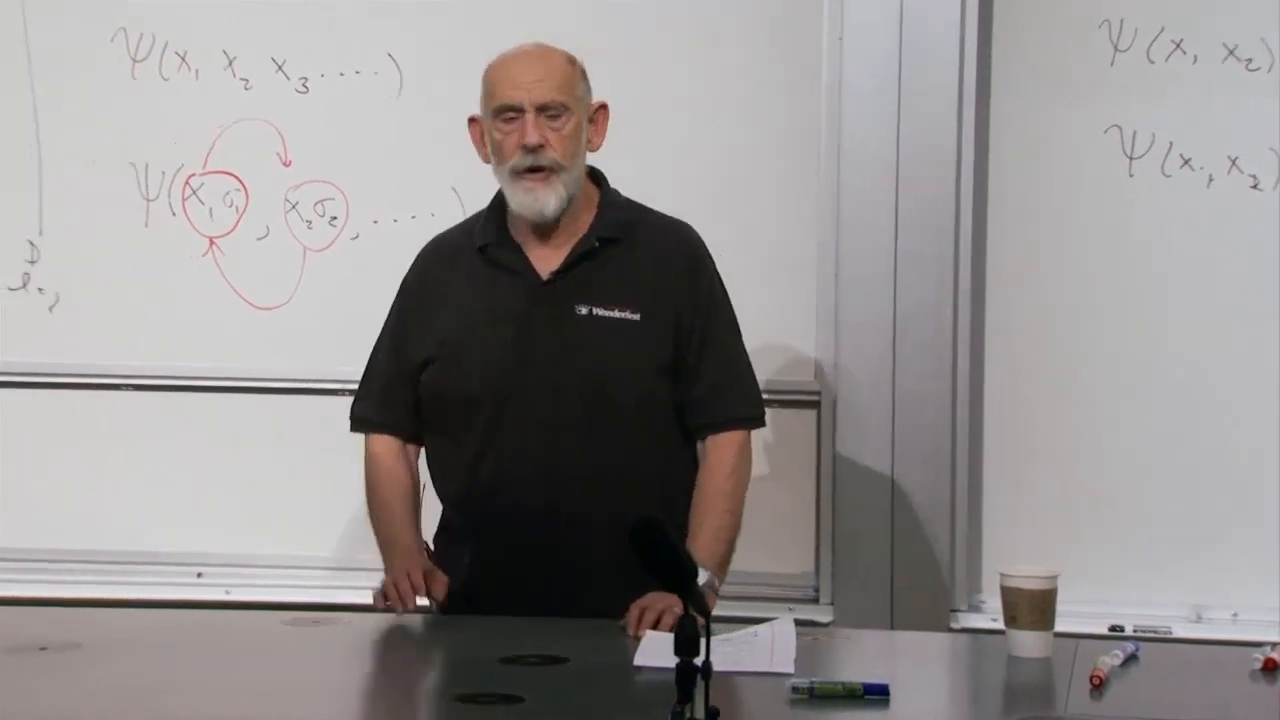
\includegraphics[width=0.9\linewidth]{lecture_05_frame_03.png}
\caption{يبدل تبادل جسيمين متماثلين وسمي الموضع--اللف المغزلي الكاملين الخاصين بهما. تبقى الحالة البوزونية بلا تغير، بينما تتغير إشارة الحالة الفرميونية.}
\lectureframe{00:35:25}
\end{figure}

هذه استخدامات مختلفة للخطية. لجسيم واحد،
\begin{equation}
\alpha\psi_0(x)+\beta\psi_1(x)
\end{equation}
هو تراكب لبديلين. ولجسيمين،
\begin{equation}
\psi_0(x_1)\psi_1(x_2)
\end{equation}
هو سعة جداء على فضاء ذي إحداثيي جسيمين. ويجمع التماثل أو مضادّة التماثل ذلك الجداء مع نظيره الناتج عن التبديل.

\begin{classroomqa}
\lecturetimestamp{00:36:13}
\audiencequestion{هل يؤدي تبديل الجسيمات إلى أثر تداخل؟}
\lecturerresponse{نعم. يمكن فهم انعدام السعة الفرميونية للحالة نفسها على أنه تداخل هدّام بين المساهمتين الناتجتين عن التبديل.}
\end{classroomqa}

\begin{classroomqa}
\lecturetimestamp{00:37:13}
\audiencequestion{هل اشتق Pauli الاستبعاد باستخدام حجة التماثل نفسها؟}
\lecturerresponse{بدأ Pauli من حقيقة تجريبية، ووجد إطارًا رياضيًا يمكن التعبير عنها فيه. ولم يكن في البداية يشتق الاستبعاد من نظرية أكثر أساسية.}
\end{classroomqa}

توفّر مضادّة التماثل الإطار الرياضي الذي تُصاغ فيه قاعدة الاستبعاد التجريبية.

\begin{classroomqa}
\lecturetimestamp{00:39:01}
\audiencequestion{هل يرتبط تداخل تبديل الجسيمات بالتداخل بين المسارات البديلة؟}
\lecturerresponse{نعم. في أحد التاريخين يمر الجسيمان من دون أن يتقاطعا، بينما في تاريخ آخر يتقاطعان فيصل كل منهما إلى وجهة الآخر. وتتجمع السعات للبوزونات، ويمكن أن تلغي بعضها بعضًا للفرميونات.}
\end{classroomqa}

يوفّر التبديل إشارة السالب الأولى. ويوفّر الدوران الثانية.

\section{إشارة السالب الثانية: الدوران بزاوية \texorpdfstring{\(2\pi\)}{2 pi}}

يبدو أن دورة كاملة لا تفعل شيئًا. فكل اتجاه هندسي عادي يعود إلى نقطة بدايته بعد زاوية \(2\pi\). غير أن ما يجب أن يعود هو الاحتمالات وقيم التوقع. أمّا متجه الحالة نفسه فقد يعود مع طور كلي، كما قد يحدث له تحت التبديل.

\begin{classroomqa}
\lecturetimestamp{00:42:12}
\audiencequestion{أي محور يُستخدم للدوران، وهل المولِّد هو العزم الزاوي المداري أم اللف المغزلي أم كلاهما؟}
\lecturerresponse{يمكن اختيار محور خارجي؛ ويؤخذ فيما يلي أنه محور \(z\). والمولِّد هو العزم الزاوي الكلي، بما في ذلك المساهمتان المدارية والمغزلية. ولا يلزم أن يكون اللف المغزلي نفسه موجّهًا على امتداد المحور المختار.}
\end{classroomqa}

\editorialnote{تستخدم صيغ العزم الزاوي في هذا النقاش \(\hbar=1\)، لذا فإن \(m\) هي القيمة الذاتية اللابعدية لـ \(J_z\).}

لنرمز بـ \(\psi(\theta)\) إلى الحالة التي نحصل عليها عندما تتقدم معلمة الدوران خلال زاوية \(\theta\). ووفق الاصطلاح المستخدم هنا،
\begin{equation}
J_z\psi(\theta)
=
-i\frac{\partial}{\partial\theta}\psi(\theta).
\end{equation}
وبالنسبة إلى حالة ذات \(J_z\) محدد،
\begin{equation}
J_z\psi(\theta)=m\psi(\theta).
\end{equation}
وبجمع المعادلتين نحصل على
\begin{equation}
-i\frac{\partial}{\partial\theta}\psi(\theta)
=
m\psi(\theta),
\end{equation}
وحلها هو
\begin{equation}
\psi(\theta)=e^{im\theta}\psi(0).
\end{equation}

القيم المسموح بها لـ \(m\) هي أعداد صحيحة أو أنصاف أعداد صحيحة. ولذلك
\begin{equation}
\psi(2\pi)
=
\begin{cases}
+\psi(0), & m\in\mathbb Z,\\[4pt]
-\psi(0), & m\in\mathbb Z+\tfrac12.
\end{cases}
\end{equation}
وبعد دورة كاملة أخرى،
\begin{equation}
\psi(4\pi)=\psi(0)
\end{equation}
في كلتا الحالتين. هذه هي إشارة السالب الثانية: فالحالة في متعدِّدة عزم زاوي نصف-صحيح تغيّر إشارتها تحت دوران مقداره \(2\pi\).

لا تغيّر الإشارة \(\lvert\psi\rvert^2\)، ولذلك لا تكون مرئية عندما تضرب الحالة بأكملها. ومع ذلك، فإن دورانًا مقداره \(2\pi\) لا يمثله مؤثر الهوية على حالة ذات لف مغزلي نصف-صحيح. ويصبح الفرق قابلاً للرصد عندما تُجعل الإشارة نسبية إلى سعة متماسكة أخرى.

\section{المساران \texorpdfstring{\(2\pi\) و\(4\pi\)}{2 pi و4 pi}}

يمكن إظهار الفرق بين \(2\pi\) و\(4\pi\) من دون مزيد من الجبر. أمسك كوبًا بيد واحدة وأدره دورة كاملة من غير أن تتركه. يعود الكوب إلى وضعه الأصلي، لكن الذراع تكون قد التوت. واصل حتى دورة ثانية، وعندئذ يمكن إعادة الذراع إلى موضعها الأصلي من دون عكس حركة الكوب.

يتضمن إنشاء ذو صلة وضع كرة داخل صندوق وربطها بالصندوق بخيوط. فإدارة الكرة بمقدار \(2\pi\) تترك تشابكًا. وفي الفضاء الثلاثي الأبعاد الاعتيادي، يمكن فك التشابك المرتبط بدوران مقداره \(4\pi\). والشيء ذو الصلة ليس مجرد الوضع النهائي للكرة، بل المسار المتبع عبر فضاء الدورانات.

\begin{classroomqa}
\lecturetimestamp{00:54:22}
\audiencequestion{إذا أُديرت الكرة مرتين حول المحور نفسه، فهل يمكن حقًا فك الخيوط من تشابكها؟ وهل يتطلب ذلك بُعدًا مكانيًا آخر؟}
\lecturerresponse{يمكن فك مسار \(4\pi\) في الفضاء الثلاثي الأبعاد الاعتيادي. فالزمن يقوم بدور معلمة للحركة؛ وليس اتجاهًا مكانيًا آخر. ولا يمكن فك مسار \(2\pi\) بهذه الطريقة، بينما يمكن فك مسار \(4\pi\).}
\end{classroomqa}

تميّز هاتان المظاهرتان بين مسار \(2\pi\) غير تافه ومسار \(4\pi\) قابل للفك، من دون تطوير نظرية صورية لزمرة الدوران.

\section{التبديل والدوران في صورة الحزام}

تقف إشارتا السالب الآن جنبًا إلى جنب. فتبديل فرميونين متماثلين يغيّر إشارة دالتهما الموجية المشتركة. كما أن تدوير حالة واحدة ذات لف مغزلي نصف-صحيح بمقدار \(2\pi\) يغيّر إشارتها أيضًا. ويعطي الحزام علاقة هندسية بين العمليتين.

رتّب الحزام بحيث يكون طرفاه السفليان قد تبدّلا. ومن منظور آخر، يحمل الحزام نفسه لفة بمقدار \(2\pi\). إن إجراء التبديل مع دوران مقداره \(2\pi\) يزيل اللفة ويترك الحزام غير ملتف. ويمكن اختزال العملية المركبة اختزالًا متصلًا إلى ألا نفعل شيئًا.\footnote{تُنسب ملاحظة التبديل--الدوران في المحاضرة إلى David Finkelstein. ولا يحدَّد أي منشور بعينه في سجل المصدر، لذلك أُبقي الاسم هنا على هذا الأساس وحده.}

\begin{classroomqa}
\lecturetimestamp{01:01:12}
\audiencequestion{أهذا مجرد وصف لكيفية تضمين الحزام في الفضاء، لا وصف لطوبولوجيا الجسيمات؟}
\lecturerresponse{يمكن قراءة الحزام بوصفه تاريخًا جسيميًا في الزمكان. ومع سير الزمن إلى الأعلى، يعطي مقطع عرضي خلاله أشياء شبيهة بالجسيمات. تُنشأ أزواج، ويُدار أحد الأجسام بمقدار \(2\pi\)، ويُبدَّل جسمان متماثلان. وفي ذلك التاريخ يلغي طورا الدوران والتبديل أحدهما الآخر.}
\end{classroomqa}

يجعل هذا التاريخ تتبّع الأطوار صريحًا. ابدأ من دون جسيمات. وفي موضعين منفصلين، أنشئ زوجًا جسيم--ضديد جسيم، فيبقى أربعة جسيمات عند زمن وسيط. أدر أحد الجسيمات بمقدار \(2\pi\) بينما تبدّل جسيمين متماثلين في موضع آخر من الترتيب. ويمكن تشويه التاريخ الكامل تشويهًا متصلًا إلى التاريخ الابتدائي الذي فيه يُنشأ زوج ثم يُفنى لاحقًا. وفي تتبّع الإشارات الجاري نقاشه، لا يحمل ذلك التاريخ التافه أي طور إضافي. وإذا كانت \(\eta_{\mathrm{rot}}\) و\(\eta_{\mathrm{ex}}\) ترمزان إلى الإشارتين، أمكن كتابة الإلغاء المذكور بإيجاز على الصورة الآتية\footnote{تسجّل معادلة الطور هذه الإلغاء الموصوف من 01:06:50 إلى 01:07:18؛ وتعرض المحاضرة هذا البناء على أنه موحٍ لا برهان صارم.}
\begin{equation}
\eta_{\mathrm{rot}}\eta_{\mathrm{ex}}=1.
\end{equation}

\begin{classroomqa}
\lecturetimestamp{01:03:34}
\audiencequestion{هل يمكن ربط التبديل بالدورانات بأن نَدَع كلًا من جسيمين يتحرك خلال \(\pi\) ثم نعيد توجيههما؟}
\lecturerresponse{قد يعكس هذا البناء رياضيات ذات صلة، لكنه يستخدم دورانين منفصلين مقدارهما \(\pi\). أمّا العملية التي تُحلَّل هنا فتتضمن دورانًا واحدًا مقداره \(2\pi\)، لذا فالحجتان ليستا متطابقتين.}
\end{classroomqa}

تعتمد الحجة على إمكان إنشاء أشياء شبيهة بالجسيمات وإفنائها. ولن تكون لها هذه الصيغة في نظرية تكون جسيماتها أزلية. وهي أيضًا لا تُقدَّم بوصفها البرهان المعياري على مبرهنة اللف المغزلي--الإحصاء. وغرضها إظهار سبب طوبولوجي لتلاؤم إشارتي التبديل والدوران.

\section{التكتلات، والصور المرآتية، والفناء}

يمكن تكرار هذا البناء مع تشكيلات حقلية موضعية. افترض أن حقلًا واحدًا أو أكثر يأخذ قيم الفراغ الخاصة به في كل مكان تقريبًا، ولكن له شكلًا وبنية غير صفريين في منطقة صغيرة. ذلك التشكيل الموضعي هو تكتل.

الآن أنشئ تشكيلًا ثانيًا بوصفه الصورة المرآتية المناسبة للأول. سمِّ أحدهما الجسيم والآخر ضديد الجسيم. قرّبهما أحدهما من الآخر. تلتقي الأجزاء المتناظرة من التشكيلين الحقليين ويبطل بعضها بعضًا. وفي مرحلة وسطى قد تكون بعض أجزاء التكتلين قد اختفت بالفعل بينما تبقى أجزاء أخرى. ومواصلة التشويه تزيل البنية المتبقية وتعيد الحقول إلى تشكيل الفراغ. وتعطي لفتان متعاكستان في حزام الصورة نفسها: ادفع اللفتين معًا فتنفكان.

يمكن إجراء العملية بالعكس. ويمكن للفضاء الخالي أن ينتج تكتلًا وقرينه المرآتي. ويمكن إنشاء زوجين من هذا النوع، وتدوير أحد التكتلات بمقدار \(2\pi\)، وتبديل تكتلين متماثلين، ثم إفناء الزوجين من جديد. وعندئذ ينطبق الإلغاء نفسه للتبديل--الدوران. ويظل هذا توسيعًا استرشاديًا للبناء، لا مبرهنة بشأن كل إثارة موضعية.

\begin{classroomqa}
\lecturetimestamp{01:11:30}
\audiencequestion{هل توجد تحققات فيزيائية لهذه التشكيلات الحقلية الشبيهة بالكتل؟}
\lecturerresponse{نعم. وتشمل الأمثلة الأنوية في الأوصاف من نمط Skyrmion، والأقطاب المغناطيسية الأحادية، وإثاراتٍ حقلية أخرى شبيهة بالجسيمات.}
\end{classroomqa}

إن صورة الكتلة وصورتها المرآتية هي ما يجعل هذا التعميم مفهومًا. والسمة ذات الصلة ليست أن الشيء بدأ بوصفه جسيمًا نقطيًا أوليًا، بل إن إثارةً شبيهةً بالجسيم وقرينتها يمكن إنشاؤهما، ثم جمعهما معًا، ثم إفناؤهما على نحو مستمر. وهذه السمة تحفز علاقة أوسع بين سلوك الدوران وسلوك التبادل.

\begin{classroomqa}
\lecturetimestamp{01:16:12}
\audiencequestion{هل يعني اللف المغزلي بمقدار نصف أن الحالة تكتسب فقط نصف طور الدوران المعتاد؟}
\lecturerresponse{الطور في هذا الاصطلاح هو \(e^{im\theta}\). وعندما تكون \(m\) نصفَ عددٍ صحيح، فإن دورانًا بمقدار \(2\pi\) يعطي \(-1\)، بينما يعطي دوران بمقدار \(4\pi\) \(+1\).}
\end{classroomqa}

\section{إشارة كلية وتجربة عدمية}

هل يمكن رصد إشارة السالب الناتجة عن دوران بمقدار \(2\pi\)؟ ابدأ بتجربة لا يمكن فيها ذلك. احبس إلكترونًا في مجال مغناطيسي، ودع لفَّه المغزلي يتبع المجال بينما يُدار الجهاز ببطء خلال \(2\pi\)، ثم أطلق الإلكترون إلى جهاز تداخل. وقارن هذا بالإجراء نفسه من دون الدوران.

يغيّر الدوران الحالة على النحو الآتي:
\begin{equation}
\psi\longmapsto-\psi,
\end{equation}
لكن إشارة السالب تضرب الحالة بأكملها. وكل احتمال يبقى بلا تغير، لذلك لا يحتفظ نمط التداخل النهائي بأي أثر لحدوث الدوران التمهيدي أو عدم حدوثه. وهذه تجربة عدمية: فالطور المشترك لا يملك ما يتداخل معه.

\begin{classroomqa}
\lecturetimestamp{01:20:01}
\audiencequestion{لماذا يجب إجراء دوران المجال المغناطيسي ببطء؟}
\lecturerresponse{يجب أن يظل اللف المغزلي متتبعًا المجال المغناطيسي الدائر. فإذا جرى سحب المجال بسرعة أكبر من اللازم، فلن يبقى اللف المغزلي مقترنًا به.}
\end{classroomqa}

\section{إلكترون واحد في فرعين متماسكين}

تصبح الإشارة قابلة للرصد حين تُجعل نسبية. أرسل إلكترونًا واحدًا عبر مقسِّم حزمة. يسلك جزء من دالته الموجية مسارًا، ويسلك جزء آخر مسارًا آخر:
\begin{equation}
\psi(x)=\psi_1(x)+\psi_2(x).
\end{equation}
هذا إلكترون واحد، لا إلكترونان. إنه تراكب متماسك لبديلين. ويجب إبقاء التمييز واضحًا: فالحزمتان ليستا جسيمين مستقلين.

وجّه الحزمتين إلى منطقتين منفصلتين تحتويان على حقول مغناطيسية. أدر المجال في إحدى المنطقتين بمقدار \(2\pi\)، واترك المجال في الأخرى دون تغيير. بالنسبة إلى حالة ذات لف مغزلي نصف صحيح،
\begin{equation}
\psi_1(x)+\psi_2(x)
\longmapsto
\psi_1(x)-\psi_2(x),
\end{equation}
حيث اختيرت تسمية الفرع الذي خضع للدوران على أنها \(2\). والإشارة الآن نسبية. وعندما تتراكب الحزمتان لاحقًا، يكون الجمع قد تحول إلى طرح. ويمكن لنقطة من التداخل البنّاء أن تصبح نقطة من التداخل الهدّام، أو حتى عقدة.

\begin{classroomqa}
\lecturetimestamp{01:23:46}
\audiencequestion{ما الذي يجري تدويره إذا كان هناك إلكترون واحد فقط ولكن فرعان للدالة الموجية؟}
\lecturerresponse{الإلكترون في تراكب متماسك لبديلين موضعيين. أحد الفرعين يُدار والآخر لا يُدار. وإذا فُتحت الصناديق لمعرفة أي البديلين قد وقع، فإن ذلك القياس يدمّر التداخل.}
\end{classroomqa}

إن فتح الصناديق لن يكشف إلا عن إلكترون واحد، في أحد الصندوقين أو الآخر. ومن دون ذلك القياس تبقى كلتا السعتين في الحالة. ويؤدي تكرار التجربة إلى تراكم نمط التداخل كشفًا بعد كشف. وعند عقدة تنتج عن إشارة السالب النسبية، لا يُكشف عن أي إلكترون.

\section{السبق المغناطيسي وتداخل الشقين}

يستعاض عن تجربة الصندوق البطيئة جدًا بترتيب تخطيطي أكثر عملية. قسّم موجة إلكترون متماسكة إلى مسارين. وفي أحد المسارين، دع الإلكترون يمر عبر منطقة مغناطيسية يكون لفّه المغزلي فيها، في البداية، متعامدًا على المجال. عندئذ يسبق اللف المغزلي. وباختيار شدة المجال وزمن العبور، يمكن للّف المغزلي في ذلك الفرع أن ينجز لفة كاملة بمقدار \(2\pi\)، بينما لا يخضع الفرع الآخر لمثل هذه اللفة.\footnote{تنص المحاضرة على أن تجربةً ذات صلة بطور السبينور قد أُجريت، وتصف مبدأها، لكن السجل المصدري لا يحدّد ورقةً بحثية ولا جهازًا بعينه. ولذلك يقتصر العرض هنا على البنية المعطاة في المحاضرة.}

\begin{classroomqa}
\lecturetimestamp{01:27:05}
\audiencequestion{كيف يمكن تحديد مسار الإلكترون المنفرد؟}
\lecturerresponse{لا يمكن تحديده من دون إفساد التجربة. فأي قياس يسجّل أيَّ مسار سلكه الإلكترون يدمّر التداخل.}
\end{classroomqa}

\begin{classroomqa}
\lecturetimestamp{01:27:50}
\audiencequestion{ما المقصود بدقة بفرع من الدالة الموجية، وكيف يُنتج المقسِّم فرعين؟}
\lecturerresponse{الفرع حزمة موجية متموضعة على امتداد أحد المسارين. ويحوّل المقسِّم الموجة الداخلة إلى حزمتين منفصلتين مكانيًا، ويمكن لحقول كهربائية أو مغناطيسية أن توجه هاتين الحزمتين على مسارات مختلفة.}
\end{classroomqa}

باستثناء المنطقة المغناطيسية، هذه هي تجربة الشقين. تنفصل موجة إلكترون داخلة إلى حزمتين. وتنتشر الموجتان الخارجتان إلى منطقة كشف مشتركة، حيث تتراكب سعتاهما. ومن دون دوران نسبي قد تتضافر السعات المركزية. أما دوران اللف المغزلي بمقدار \(2\pi\) في أحد المسارين فيعكس إشارة إحدى السعات، ويمكن أن يجعل المساهمات نفسها تلغي بعضها بعضًا.

\begin{classroomqa}
\lecturetimestamp{01:30:46}
\audiencequestion{كيف يمكن أن يحدث تداخل إذا كان الإلكترون ينتقل عبر أنابيب أو شقوق منفصلة؟}
\lecturerresponse{إن الكشف النهائي لا يكشف عن المسار. تنتشر سعتا الموجة الخارجتان وتتراكبان عند الكاشف. أما النظر لمعرفة أيَّ مسار قد سلكه فسيُفسد التداخل.}
\end{classroomqa}

\begin{classroomqa}
\lecturetimestamp{01:33:22}
\audiencequestion{هل يجب أن يكون قطر الأنبوب أو الشق مقارنًا بطول موجة الإلكترون؟}
\lecturerresponse{في تحقيق حرفي لتجربة الشقين قائم على الحيود، يجب أن تكون الفتحة صغيرة بما يكفي لإنتاج الانتشار المطلوب. أما الجهاز الموصوف هنا فهو تخطيطي لا تصميم عملي.}
\end{classroomqa}

\begin{classroomqa}
\lecturetimestamp{01:33:44}
\audiencequestion{هل يترك دوران استقطاب الفوتونات الموافق بمقدار \(2\pi\) نمط التداخل من دون تغير؟}
\lecturerresponse{نعم. فالفوتونات ذات لف مغزلي صحيح، ولذلك فإن دورانًا كاملاً بمقدار \(2\pi\) لا يُدخل إشارة السالب الفرميونية.}
\end{classroomqa}

\begin{classroomqa}
\lecturetimestamp{01:34:12}
\audiencequestion{ما الاختلاف الطفيف بين التجربة العملية والنسخة المثالية؟}
\lecturerresponse{في البناء المثالي يُدار اللف المغزلي أديباتيًا. أما في الوصف العملي فيتحرك الإلكترون عبر منطقة مغناطيسية ويسبق لفّه المغزلي بسرعة أكبر، لكن الطور المقاس يظل هو الطور المرتبط بلفة مقدارها \(2\pi\).}
\end{classroomqa}

يعزل الترتيب البطيء الفكرةَ بضمان أن اللف المغزلي يتبع المجال من دون حركة إضافية. ويصل ترتيب السبق إلى الإشارة النسبية نفسها ديناميكيًا. وفي أيٍّ من النسختين، يجب أن يكفّ المساران عن كونهما قابلين للتمييز قبل أن يظهر نمط تداخل.

\begin{classroomqa}
\lecturetimestamp{01:36:15}
\audiencequestion{هل يجب إعادة جمع الفرعين بعد المقسِّم؟}
\lecturerresponse{نعم. يجب أن تتراكب الحزمتان الموجيتان الناشئتان، أو أن تنتشرا على منطقة كشف مشتركة، بحيث تستطيع سعتاهما تكوين نمط تداخل.}
\end{classroomqa}

\begin{classroomqa}
\lecturetimestamp{01:38:12}
\audiencequestion{هل تجربة دوران الإلكترون الواحد هذه نتيجة لمبدأ استبعاد باولي؟}
\lecturerresponse{لا. فهناك إلكترون واحد فقط. تقيس التجربة طور السبينور تحت الدوران، لا استبعاد فرميونين من حالة واحدة.}
\end{classroomqa}

\section{تداخل التبادل والدوران النسبي}

يمكن كشف إشارة التبادل بالطريقة العامة نفسها، مع أن الجهاز المقترح أعقد. ابدأ بإلكترونين وقسّم دالتهما الموجية المشتركة إلى فرعين متماسكين. وما يزال هناك إلكترونان فقط، لا أربعة: فالزوج يسلك أحد البديلين أو الآخر. أجرِ تبادلاً بين الإلكترونين في أحد الفرعين واتركهما في الآخر من دون تبادل. وبعد إعادة جمع الفرعين، تظهر إشارة التبادل الفرميونية بوصفها طورًا نسبيًا، ويمكنها أن تغيّر التداخل.

يقارن الاقتراح الأخير بين إشارتي السالب مباشرةً. يكتسب أحد الفرعين طور التبادل الفرميوني، بينما يكتسب الآخر طور الدوران الموافق بمقدار \(2\pi\). وكلا الطورين يساويان \(-1\)، ولذلك يزول الأثر النسبي.\footnote{يوضح التسجيل بين 01:40:26 و01:41:15 بوضوح طورَ تبادل، وطورَ دوران بمقدار \(2\pi\)، وإلغاءَ أحدهما للآخر، لكن التعيين التفصيلي للدوران لا يمكن استخلاصه من الكلام المتاح.} وتعرض المحاضرة هذا على أنه تجربة فكرية مقترحة، وتقول إنه، بحسب علم المتحدث، لم تُجرَ.

\begin{classroomqa}
\lecturetimestamp{01:41:34}
\audiencequestion{هل إن رصد طور تبادل من شأنه أن يُشكِّك في عدم قابلية التمييز بين الإلكترونين؟}
\lecturerresponse{لا. إن عدم قابلية التمييز الكمومي أدق من التطابق الكلاسيكي. فهو يسمح لمتجه الحالة بأن يغيّر إشارته تحت التبادل، مع أنه لا يوجد أي وسم قابل للرصد يميّز بين الجسيمين.}
\end{classroomqa}

هناك قيد أخير. إن تدوير عالمٍ معزولٍ بأكمله بمقدار \(2\pi\) لن يسفر إلا عن طورٍ مشترك، ولن تستطيع أي تجربة داخلية كشفه. أما التجربة القابلة للرصد فتُخضِع أحد الفرعين المتماسكين لدوران بالنسبة إلى الآخر. ولذلك فإن ما يُرصَد ليس إشارةً مطلقة، بل التداخل الناجم عن إشارة نسبية.

\chapter{المذبذبات، وأعداد الإشغال، وأول حقل كمي}

نظرية الحقول الكمومية هي إطارنا لما يقرب من كل الفيزياء غير الثقالية المعروفة. ولا ينبغي الخلط بين هذه الدعوى وبين دعوى أن كل مسألة يمكن حلها. فذرة الهيدروجين قابلة للمعالجة؛ وبحلول الوقت الذي نصل فيه إلى ذرة مثل البورون، يكون الحساب قد صار أشد صعوبة بالفعل، أما الكائن البشري فهو أبعد بكثير من أي حساب واقعي في نظرية الحقول. وقد يكون الإطار أساسيًا في حين تظل معادلاته شديدة الصعوبة إلى حد كاسح.

لذلك سندخل الموضوع بأبسط طريقة أولية ممكنة. ويُسمى هذا الموضوع أحيانًا \emph{التكميم الثاني}، لكن الاسم لن يعني الكثير حتى نبني الأدوات اللازمة. وأقصر طريق لا يبدأ بحقل نسبي، بل بالمذبذب التوافقي. فليست النوابض هي المقصودة. وإنما المهم هو جبر مؤثري الرفع والخفض. وما إن يُكرَّر هذا الجبر على أنماط كثيرة حتى يكف مؤثر الرفع عن أن يعني مجرد ``رفع مذبذب بمقدار مستوى واحد''، ويعني حرفيًا ``خلق جسيم.''

\section{المذبذب بوصفه جبرًا}

بالنسبة إلى مذبذب واحد، ليكن \(a^\dagger\) يرفع الإثارة، وليكن \(a\) يخفضها. والترميز \(a_+\) و\(a_-\) مكافئ، لكن ترميز الخنجر يستبق اللغة المستخدمة في نظرية الحقول. أما الحالة الدنيا فتخضع لـ
\begin{equation}
a|0\rangle=0,
\end{equation}
وعامل العدد هو
\begin{equation}
N=a^\dagger a,
\qquad
N|n\rangle=n|n\rangle.
\end{equation}
ومؤثرا السلم هذان مترافقان هيرميتيًا، ومبدلهما الأساسي هو
\begin{equation}
[a,a^\dagger]=1.
\label{eq:l06-single-commutator}
\end{equation}
وهذا الجبر الصغير يكاد يكون المذبذب كله.

يمكن استرجاع \(a\) و\(a^\dagger\) من تراكيب خطية مناسبة للموضع والزخم. ويعتمد الاصطلاح الدقيق على تطبيع \(x\) و\(p\) و\(m\) و\(\omega\)؛ أما العبارة الثابتة المفيدة هنا فهي أن \(a^\dagger a\) يعيد بناء هاميلتوني المذبذب التربيعي باستثناء طاقة حالته القاعية المضافة. ومن ثم
\begin{equation}
H=\hbar\omega\left(N+\frac12\right).
\end{equation}
وفي مناقشتنا الحالية نهمل الحد الثابت ونعمل مع
\begin{equation}
H=\hbar\omega N.
\label{eq:l06-one-oscillator-hamiltonian}
\end{equation}
ويخبرنا التردد بكلفة إثارة واحدة. فزيادة \(n\) بمقدار واحد تكلف \(\hbar\omega\)؛ وإنقاص \(n\) بمقدار واحد يحرر المقدار نفسه.

\section{مذبذبات مستقلة كثيرة}

والآن خذ مذبذبات كثيرة ووسمها بـ \(i\). وهذه العلامة مجرد مؤشر، لا الوحدة التخيلية. وقد يكون عدد الأنماط منتهيًا أو لا نهائيًا. وتعطي مجموعة من النوابض المستقلة صورةً واحدة؛ وتعطي الأنماط العادية لوتر كمان مثالي صورةً أخرى. وفي تطبيقات نظرية الحقول تكون المجموعة اللانهائية هي الحالة المهمة.

للاستقلال معنى مؤثري. فالمؤثرات التي تنتمي إلى منظومات فرعية مستقلة حقًا تتبادل. ولو لم تفعل ذلك، لما أمكن قياس الكميات الموافقة على نحو مستقل، ولما كانت الأنظمة مستقلة أصلًا. لذلك يكون لدينا
\begin{align}
[a_i,a_j]&=0, \\
[a_i^\dagger,a_j^\dagger]&=0, \\
[a_i,a_j^\dagger]&=\delta_{ij}.
\label{eq:l06-many-commutators}
\end{align}
وعندما يكون \(i\ne j\)، فإن كل ما يخص النمطين يتبادل. وعندما يكون \(i=j\)، يؤول السطر الأخير إلى المعادلة~\eqref{eq:l06-single-commutator}.

لكل مذبذب عامل عدده الخاص، وله أيضًا، بوجه عام، تردده الخاص:
\begin{equation}
N_i=a_i^\dagger a_i,
\qquad
H=\sum_i\hbar\omega_i N_i.
\label{eq:l06-many-hamiltonian}
\end{equation}
وتُوسم الحالة الذاتية المشتركة بالقائمة الكاملة
\begin{equation}
|n_1,n_2,n_3,\ldots\rangle,
\qquad n_i=0,1,2,\ldots.
\label{eq:l06-occupation-ket}
\end{equation}
ويُسمى العدد الصحيح \(n_i\) \emph{عدد الإشغال} للمذبذب رقم \(i\). وفي هذه المرحلة ليس ذلك إلا اصطلاحًا. وسرعان ما سيعد الجسيمات التي تشغل حالة جسيم واحد، وعندئذ سيصبح الاسم حرفيًا.

والحالة التي يساوي فيها كل عدد إشغال صفرًا هي
\begin{equation}
|0\rangle\equiv|0,0,0,\ldots\rangle,
\qquad a_i|0\rangle=0\quad\text{for every }i.
\label{eq:l06-oscillator-vacuum}
\end{equation}

\begin{classroomqa}
\lecturetimestamp{00:15:27}
\audiencequestion{هل تقابل عائلة لا نهائية من المذبذبات مجموعةً متصلةً من الأنماط في نظام مثل وتر كمان؟}
\lecturerresponse{نعم، في الوتر المثالي. فالوتر الحقيقي مكوَّن من ذرات، ولذلك تصادف الأطوال الموجية القصيرة بما يكفي حدَّ قطع مجهريًا في نهاية المطاف. ومع ذلك فإن نموذج المتصل هو ما يحفز المجموعة اللانهائية من الأنماط المستخدمة في نظرية الحقول.}
\end{classroomqa}

\section{لماذا تكون معاملات السلم جذورًا تربيعية}

لا بد أن يرفع فعل \(a^\dagger\) حالةً ذاتيةً لـ \(N\) إلى الحالة الذاتية التالية، لكن التطبيع يترك مجالًا لمعامل:
\begin{equation}
a^\dagger|n\rangle=c_n|n+1\rangle.
\label{eq:l06-unknown-coefficient}
\end{equation}

\begin{figure}[htbp]
\centering
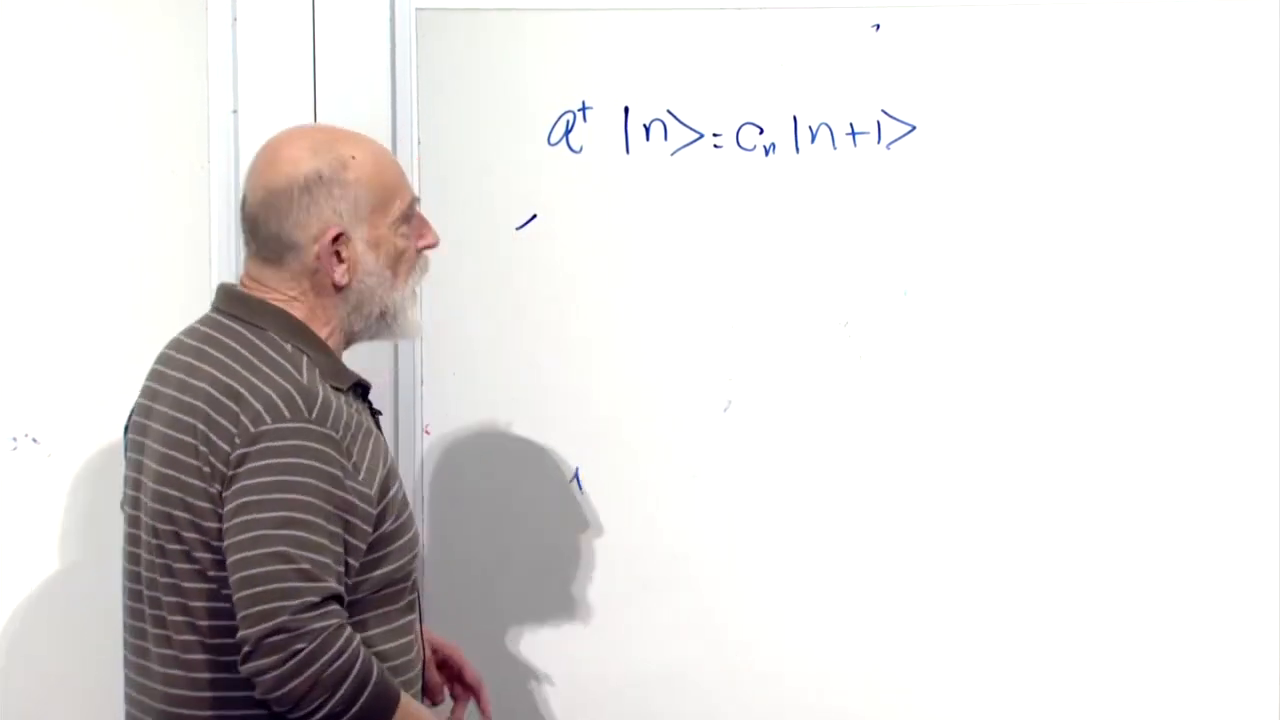
\includegraphics[width=0.9\linewidth]{lecture_06_frame_01.png}
\caption{يُدخَل معامل السلم قبل اشتقاق تطبيعه. وتُعاد كتابة المعادلة المكتوبة على اللوح في المعادلة~\eqref{eq:l06-unknown-coefficient}.}
\lectureframe{00:19:38}
\end{figure}

نختار اصطلاح الطور الذي يكون فيه \(c_n\) حقيقيًا. ويعطي أخذ المرافق الهيرميتي
\begin{equation}
\langle n|a=c_n\langle n+1|.
\end{equation}
وبضرب العلاقتين واستعمال حالات أساس مطبَّعة، نحصل على
\begin{align}
c_n^2
&=\langle n|aa^\dagger|n\rangle \\
&=\langle n|(a^\dagger a+1)|n\rangle \\
&=\langle n|(N+1)|n\rangle \\
&=n+1.
\end{align}
وبالتالي،
\begin{equation}
a^\dagger|n\rangle=\sqrt{n+1}\,|n+1\rangle.
\label{eq:l06-raising-rule}
\end{equation}

\begin{classroomqa}
\lecturetimestamp{00:22:35}
\audiencequestion{لماذا يجوز وضع \(\langle n+1|n+1\rangle=1\) قبل إيجاد \(c_n\)؟}
\lecturerresponse{تُختار المتجهات الذاتية منذ البداية على أنها أساس مطبَّع. ولا يحدد تطبيعها تطبيع \(a^\dagger|n\rangle\)؛ وهذه المعلومة المتبقية هي بالضبط المعامل \(c_n\).}
\end{classroomqa}

وتنتج قاعدة الخفض بالطريقة نفسها:
\begin{equation}
a|n\rangle=\sqrt n\,|n-1\rangle.
\label{eq:l06-lowering-rule}
\end{equation}
وعند \(n=0\)، ينعدم المعامل تلقائيًا، ولذلك تتضمن القاعدة \(a|0\rangle=0\). ومع وجود أنماط كثيرة، لا يغير المؤثر إلا عدد الإشغال في خانته الخاصة:
\begin{align}
a_i^\dagger|n_1,\ldots,n_i,\ldots\rangle
&=\sqrt{n_i+1}\,|n_1,\ldots,n_i+1,\ldots\rangle, \\
a_i|n_1,\ldots,n_i,\ldots\rangle
&=\sqrt{n_i}\,|n_1,\ldots,n_i-1,\ldots\rangle.
\label{eq:l06-multimode-ladders}
\end{align}
ولا يحدث شيء للخانات الأخرى.

\section{الدالة الموجية ليست حقلًا كموميًا}

قبل تعريف الحقل، علينا أن نميّزه عن الدالة الموجية المألوفة. وثلاثة أوجه تباين تنظّم هذا الانتقال.

أولًا، إن دالة موجية لجسيم واحد
\begin{equation}
\psi(x)=\langle x|\psi\rangle
\end{equation}
هي تمثيل لمتجه حالة. وهي ليست بنفسها كمية قابلة للرصد. فنحن نقيس الموضع، والزخم، والعزم الزاوي، وغير ذلك من المؤثرات؛ والدالة الموجية تزودنا بالسعات التي تُحسب منها احتمالات تلك النواتج.

ثانيًا، تعتمد الدالة الموجية لكثير من الجسيمات على مواضع جميع الجسيمات. وبالنسبة إلى جسيمين يُسمى متجها موضعيهما مؤقتًا \(x\) و\(y\)، يكون لدينا
\begin{equation}
\psi(x,y)=\langle x,y|\psi\rangle.
\end{equation}
وهنا يشير \(x\) و\(y\) إلى جسيمين مختلفين؛ وليسا المركبتين الديكارتيتين \(x\) و\(y\) لمتجه موضع واحد. ومع وجود \(N\) جسيمات، تُمثَّل الحالة بـ
\begin{equation}
\psi(x_1,x_2,\ldots,x_N).
\end{equation}

ثالثًا، تصف هذه الدالة الموجية عددًا ثابتًا من الجسيمات. فالدالة الموجية لخمسة عشر جسيمًا لها خمسة عشر وسيطًا موضعيًا، وتنتمي إلى فضاء هيلبرت لخمسة عشر جسيمًا. وهي لا تصف بذاتها عملية يتغير فيها العدد من خمسة عشر إلى أربعة عشر أو ستة عشر.

سيعكس الحقل الكمي هذه السمات. فهو مؤثر لا حالة، ويعتمد على نقطة مكانية واحدة \(x\)، ويؤثر في فضاء حالات يحتوي كل قطاع من قطاعات عدد الجسيمات. ويعني التعبير ``نقطة واحدة'' متجه موضع واحدًا متغيرًا بحرية. ولا يعني أن \(x\) قد أُسنِدت إليه قيمة عددية واحدة.

وهناك قيد واحد سيهم لاحقًا. فالحقل \(\Psi(x)\) الذي سيُدخَل أدناه ليس هيرميتيًا، ولذلك فهو ليس بنفسه كمية قابلة للرصد بالمعنى الصارم. أما تراكيبه الهيرميتية فهي كميات قابلة للرصد. ومن ثم فإن العبارة المؤقتة القائلة إن الحقل قابل للقياس تُصقل ولا تُطرح جانبًا: فالحقول دوال ذات قيم مؤثرية، وتراكيبها الهيرميتية تمثل كميات قابلة للقياس.

\begin{classroomqa}
\lecturetimestamp{00:36:52}
\audiencequestion{إذا كان الحقل دالة في موضع واحد، فهل يجوز لذلك الموضع أن يتغير؟ وماذا حدث لـ \(y\) في الدالة الموجية ذات الجسيمين؟}
\lecturerresponse{تتغير النقطة \(x\) على امتداد الفضاء كله. إن ``موضعًا واحدًا'' يعني أن للمؤثر وسيطًا مكانيًا واحدًا، لا أن هذا الوسيط ثابت. وفي \(\psi(x,y)\)، يسمي الرمزان \(x\) و\(y\) موضعي جسيمين؛ وبصورة مكافئة هما \(x_1\) و\(x_2\). وليسا مركبتين ديكارتيتين لوسيط الحقل.}
\end{classroomqa}

\begin{classroomqa}
\lecturetimestamp{00:38:15}
\audiencequestion{كيف يرتبط وصف الدالة الموجية ذات العدد الثابت من الجسيمات بوصف الحقل، وهل يصفان أنواعًا مختلفة من الجسيمات؟}
\lecturerresponse{هذا الارتباط هو البنية المركزية التي لم تأت بعد. والجسيمات من النوع نفسه. وفي هذه المحاضرة هي بوزونات؛ أما الفرميونات فتتطلب جبرًا مختلفًا.}
\end{classroomqa}

\section{جسيم واحد في صندوق}

لنعد مؤقتًا إلى ميكانيكا الكم العادية لجسيم واحد. ضع جسيمًا في صندوق أحادي البعد. ومع وجود جسيم واحد فقط، يصبح التمييز بين البوزون والفرميون غير ذي صلة: إذ لا يوجد جسيم مطابق ثانٍ يمكن به اختبار التبادل أو الاستبعاد.

لتكن
\begin{equation}
\psi_1(x),\ \psi_2(x),\ \psi_3(x),\ldots
\end{equation}
هي الدوال الذاتية للطاقة. فالنمط الأدنى هو أكثر موجة سلاسةً وتنعدم عند الجدران. وللنمط التالي عقدة داخلية واحدة، أما الأنماط الأعلى طاقة فتتذبذب بسرعة أكبر. وفي البئر المربعة اللانهائية المثالية ذات العرض \(L\)، فإن أساسًا مطبَّعًا مناسبًا هو
\begin{equation}
\psi_i(x)=\sqrt{\frac{2}{L}}\sin\!\left(\frac{i\pi x}{L}\right),
\qquad 0<x<L.
\label{eq:l06-box-basis}
\end{equation}
وصيغة الجيب الصريحة هذه تجسيد قياسي للرسم التخطيطي النوعي على اللوح؛ أما الحجة أدناه فلا تتطلب إلا مجموعة كاملة متعامدة ومتطبعة من حالات الجسيم الواحد.

\begin{figure}[htbp]
\centering
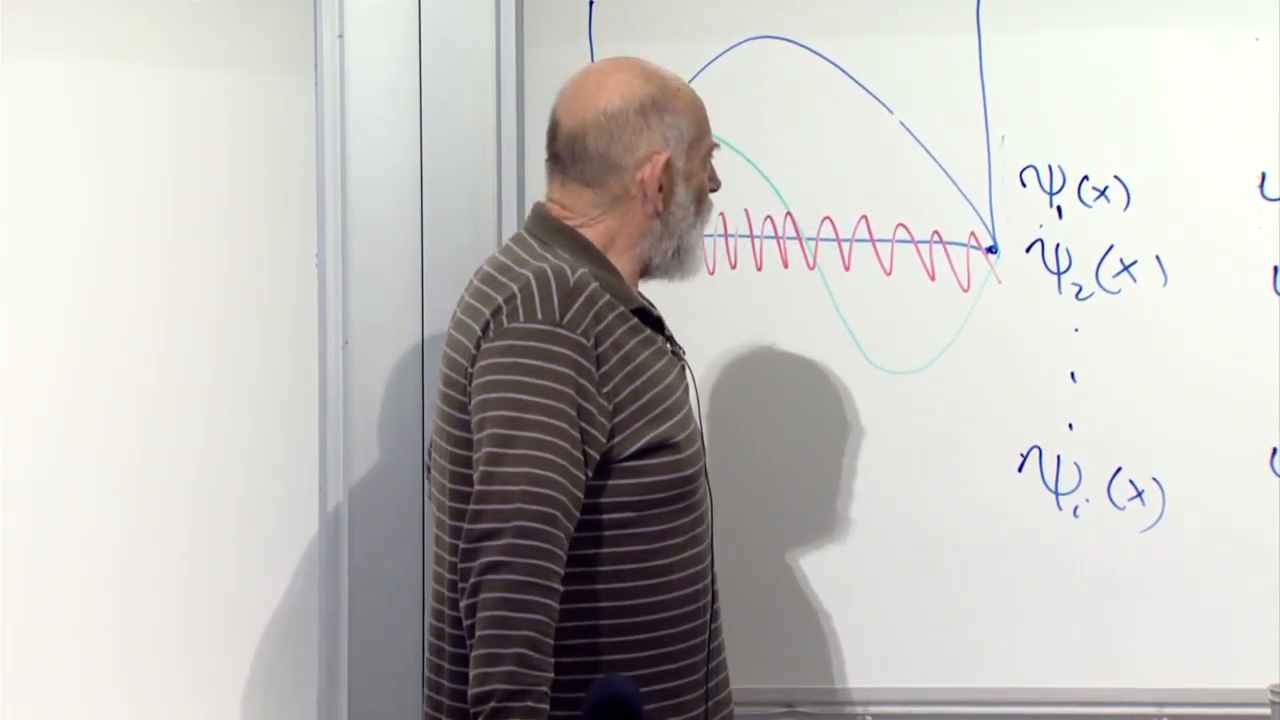
\includegraphics[width=0.9\linewidth]{lecture_06_frame_03.png}
\caption{أنماط الصندوق لجسيم واحد مرتبة بحسب تزايد الطاقة. لا يحتوي النمط الأول على أي عقدة داخلية، ويحتوي الثاني على عقدة واحدة، أما الأنماط الأعلى المحذوفة فتتذبذب بسرعة أكبر على نحو متزايد.}
\lectureframe{00:43:10}
\end{figure}

يمكن إعادة رسم البنية نفسها من دون الحجب الذي تسببه السبورة أثناء المحاضرة:
\begin{figure}[htbp]
\centering
\begin{tikzpicture}[x=1cm,y=1cm]
  \draw[thick] (0,0) -- (0,3.8);
  \draw[thick] (7,0) -- (7,3.8);
  \draw[gray!55] (0,2.75) -- (7,2.75);
  \draw[gray!55] (0,1.35) -- (7,1.35);
  \draw[blue!75!black,thick,domain=0:7,samples=120]
    plot (\x,{2.75+0.62*sin(180*\x/7)});
  \draw[teal!70!black,thick,domain=0:7,samples=120]
    plot (\x,{1.35+0.55*sin(360*\x/7)});
  \node[right] at (7.15,3.15) {$\psi_1(x)$};
  \node[right] at (7.15,1.70) {$\psi_2(x)$};
  \node at (3.5,0.45) {$\vdots\quad \psi_i(x)$};
\end{tikzpicture}
\caption{إعادة بناء نظيفة للرسم التخطيطي الكيفي لأنماط الصندوق. تفصل الإزاحة العمودية بين الدوال الذاتية لتسهيل القراءة، وليست إحداثيًا فيزيائيًا إضافيًا.}
\end{figure}

يشير الدليل \(i\) إلى حالة أحادية الجسيم، لا إلى جسيم ولا إلى عدد العقد. وفي أساس الصندوق، يصادف أن يكون \(i\) أكبر بواحد من عدد العقد الداخلية. ولكل حالة طاقة \(\varepsilon_i\). واتباعًا لترميز المحاضرة، يمكننا أن نكتب هذه الطاقة على صورة \(\hbar\omega_i\)، أو ببساطة \(\omega_i\) بعد وضع \(\hbar=1\).

\begin{classroomqa}
\lecturetimestamp{00:39:01}
\audiencequestion{هل كان افتراض الاستقلال السابق دقيقًا تمامًا، وهل يمكن أن يوسم الدليل \(i\) الحالات الممكنة لإلكترون في ذرة؟}
\lecturerresponse{في بناء الأنماط المستقلة تكون علاقات الإبدال بين الأنماط المختلفة دقيقة تمامًا. ويمكن للدليل أن يوسم حالات ذرية أحادية الجسيم. أما إذا تفاعلت الجسيمات، فإن هاملتوني الأنماط المستقلة البسيط لا يعود هو الوصف الكامل.}
\end{classroomqa}

\begin{classroomqa}
\lecturetimestamp{00:40:34}
\audiencequestion{هل الجسيم في الصندوق بوزون؟}
\lecturerresponse{قد يكون كذلك، لكن مع جسيم واحد لا يهم الإحصاء. ولا يكتسب الاستبعاد والتبادل معنى إلا عندما يوجد أكثر من جسيم متماثل واحد.}
\end{classroomqa}

\section{من أنماط الصندوق إلى فضاء فوك}

لنسمح الآن بأي عدد من البوزونات المتماثلة في الصندوق. قد يشغل عدد ما \(n_1\) الحالة \(\psi_1\)، وقد يشغل عدد ما \(n_2\) الحالة \(\psi_2\)، وهكذا. ومن ثم تكون حالة أساس هي
\begin{equation}
|n_1,n_2,n_3,\ldots\rangle.
\end{equation}
وهذا هو بالضبط الترميز المستخدم من قبل لعدد كبير من المهتزات. والتطابق هنا بنيوي: اربط مهتزًا واحدًا بكل حالة أحادية الجسيم، واعتبر عدد إثارة المهتز هو عدد الجسيمات التي تشغل تلك الحالة.

البوزونات أساسية هنا لأن كل \(n_i\) يمكن أن يكون أي عدد صحيح غير سالب. أما في حالة الفرميونات، فكل حالة أحادية الجسيم يمكن أن تكون فارغة أو مشغولة بجسيم واحد فقط، ولا يمكن أن تكون مشغولة بجسيمين، لذلك لا يمكن استعمال جبر المهتز المعتاد من غير تعديل.

يمكن الآن تعريف المؤثرات من خلال فعلها على أساس أعداد الإشغال. فالمؤثر \(a_i^\dagger\) يخلق جسيمًا واحدًا في الحالة أحادية الجسيم \(i\)؛ و\(a_i\) يزيل جسيمًا واحدًا:
\begin{align}
a_i^\dagger|n_1,\ldots,n_i,\ldots\rangle
&=\sqrt{n_i+1}\,|n_1,\ldots,n_i+1,\ldots\rangle, \\
a_i|n_1,\ldots,n_i,\ldots\rangle
&=\sqrt{n_i}\,|n_1,\ldots,n_i-1,\ldots\rangle.
\end{align}
وليست هذه مجرد مماثلة لاحقة. بل هذا هو تعريف مؤثري الخلق والفناء البوزونيين على هذا الأساس. وبما أن هذا الأساس يمتد على الفضاء، فإن التعريف يحدد فعلهما على كل حالة بالخطية.

\begin{classroomqa}
\lecturetimestamp{00:47:11}
\audiencequestion{هل \(n_1,n_2,n_3\) هي الحالات الكمومية؟}
\lecturerresponse{تحدد الوسوم \(1,2,3,\ldots\) الحالات أحادية الجسيم. أما الرموز \(n_1,n_2,n_3,\ldots\) فهي أعداد الجسيمات التي تشغل تلك الحالات. والحفاظ على التمييز بين وسم الحالة وعدد إشغالها هو العبء الترميزي الرئيسي.}
\end{classroomqa}

\subsection{ما الذي يفعله الجذر التربيعي}

العامل \(\sqrt{n_i+1}\) لا يمثل جسيمًا إضافيًا ولا عملية فيزيائية منفصلة. بل يمنح المؤثر التطبيع الصحيح والبنية الجبرية الصحيحة. وفي نمط واحد،
\begin{align}
a a^\dagger|n\rangle
&=a\bigl(\sqrt{n+1}\,|n+1\rangle\bigr) \\
&=(n+1)|n\rangle,
\end{align}
بينما
\begin{equation}
a^\dagger a|n\rangle=n|n\rangle.
\end{equation}
ومن ثم يكون الفرق بينهما هو \(|n\rangle\)، كما تقتضيه \([a,a^\dagger]=1\). وعلى نحو تقريبي جدًا، يكون كل من مؤثري السلم من رتبة \(\sqrt n\)، لأن حاصل ضربهما يعطي مؤثر العدد من رتبة \(n\).

\begin{classroomqa}
\lecturetimestamp{00:47:52}
\audiencequestion{ما المعنى الفيزيائي الملموس لعامل الجذر التربيعي؟}
\lecturerresponse{إنه في المقام الأول تطبيع رياضي. فهو يضمن أن حالات الإشغال مطبعة، وأن \(a^\dagger a\) له القيمة الذاتية \(n\)، وأن مؤثري السلم يحققان علاقة إبدال المهتز. أحيانًا تكون الرياضيات هي المعنى الذي نحتاج إليه.}
\end{classroomqa}

\begin{classroomqa}
\lecturetimestamp{00:52:25}
\audiencequestion{هل جرى تعريف مؤثري الخلق والفناء فقط من خلال خواصهما وفعلهما على الأساس؟}
\lecturerresponse{نعم. لا يلزم أن تنشأ التعريفات من تصور أكثر بدائية. وتختبر قيمتها بنتائجها. إن تعريف الفعل على أساس كامل يحدد المؤثرات على فضاء فوك كله، وهذه التعريفات تعيد إنتاج علاقات الإبدال المطلوبة.}
\end{classroomqa}

\begin{classroomqa}
\lecturetimestamp{00:53:22}
\audiencequestion{لماذا يجعل \(a_i\) جسيمًا يختفي بدلًا من أن ينقله فحسب إلى حالة مختلفة؟}
\lecturerresponse{لأن \(a_i\) معرَّف على أنه ينقص إشغال الحالة \(i\). والسؤال المفيد ليس لماذا يكون التعريف صحيحًا، بل لماذا يكون مفيدًا. وهو مفيد لأن الانبعاث والامتصاص يتطلبان مؤثرات تغيّر عدد الجسيمات: فالفوتون يُخلَق عند انبعاث الإشعاع ويُفنى عند امتصاصه.}
\end{classroomqa}

الفضاء الممتد بواسطة جميع حالات أعداد الإشغال هو \emph{فضاء فوك}. وهو يحتوي على الخلاء، وكل حالة أحادية الجسيم، وكل حالة ثنائية الجسيم، وهكذا من غير حد أعلى ثابت:
\begin{equation}
\mathcal F=\mathcal H_0\oplus\mathcal H_1\oplus\mathcal H_2\oplus\cdots.
\label{eq:l06-fock-space}
\end{equation}
ويُظهر ترميز المجموع المباشر صراحةً ما لم تُظهره دالة الموجة المعتادة ذات \(N\) جسيمًا: فجميع قطاعات عدد الجسيمات تنتمي إلى فضاء حالة واحد.

\begin{classroomqa}
\lecturetimestamp{00:54:56}
\audiencequestion{هل يؤدي تعريف المؤثرات على المتجهات الذاتية لعدد الإشغال إلى تحديدها على متجهات اعتباطية، وهل تتبع بعد ذلك علاقات إبدال المهتز؟}
\lecturerresponse{بالضبط. فمتجهات الإشغال تشكل أساسًا، لذا تمد الخطية التعريف إلى فضاء فوك كله. والتحقق من علاقات الإبدال البوزونية يتم بفعل المؤثرات على ذلك الأساس. وتمثل كل حالة أحادية الجسيم بمهتز واحد، ويكون إشغال ذلك المهتز هو عدد الجسيمات في تلك الحالة.}
\end{classroomqa}

\subsection{الخلاء والهاملتوني الحر}

خلاء فوك هو الحالة التي لا يوجد فيها أي جسيم في أي حالة أحادية الجسيم:
\begin{equation}
|0\rangle=|0,0,0,\ldots\rangle,
\qquad a_i|0\rangle=0.
\end{equation}
وقد تكون كلمة \emph{الحالة القاعية} مضللة هنا. فأدنى حالة \emph{أحادية الجسيم} هي النمط \(i=1\)؛ ولا يوجد في خلاء فوك أي جسيم حتى في ذلك النمط. وإذا شغل جسيم النمط الأدنى، أمكن لـ \(a_1\) أن يزيله ويعيد النظام إلى الخلاء.

\begin{classroomqa}
\lecturetimestamp{00:56:19}
\audiencequestion{ما الخلاء بلغة عدد الإشغال؟ وهل تكون أدنى حالة أحادية الجسيم مشغولة؟}
\lecturerresponse{في الخلاء يكون كل عدد إشغال مساويًا للصفر، ويفنيه كل \(a_i\). وأدنى نمط أحادي الجسيم غير مشغول في الخلاء. ولو كان مشغولًا، لأمكن لمؤثر إفنائه أن يزيل ذلك الجسيم.}
\end{classroomqa}

بالنسبة إلى الجسيمات غير المتفاعلة، تكون الطاقة الكلية هي مجموع المساهمات. فإذا كانت طاقة جسيم واحد في الحالة \(i\) هي \(\hbar\omega_i\)، فإن
\begin{align}
H
&=\sum_i \hbar\omega_i N_i \\
&=\sum_i \hbar\omega_i a_i^\dagger a_i.
\label{eq:l06-free-fock-hamiltonian}
\end{align}
وهناك قراءتان متكافئتان لذلك. فهو مجموع طاقات المهتزات، مهتز واحد لكل حالة أحادية الجسيم. وهو أيضًا مجموع الطاقات أحادية الجسيم، مضروبةً كل منها في عدد الجسيمات التي تحمل تلك الطاقة.

في ترميز نظرية الحقل، يُسمَّى \(a_i^\dagger\) عادةً مؤثر الخلق، ويُسمَّى \(a_i\) مؤثر الفناء. أما الترميز الأقدم \(a_+\) و\(a_-\) فيعني الشيء نفسه.

\section{توضيحات قبل أن يظهر الحقل}

تُميِّز عدة أسئلة بعد الاستراحة بين طريقة تتبّع المهتزات الجديدة هذه وبين جسيم عادي يتحرك في كمون مهتز.

\begin{classroomqa}
\lecturetimestamp{01:06:09}
\audiencequestion{إن مستويات طاقة جسيم في صندوق ليست متساوية التباعد، فأين المهتز التوافقي؟}
\lecturerresponse{لا يلزم أن تكون الطاقات أحادية الجسيم \(\omega_i\) متساوية التباعد. لكن، لكل نمط ثابت \(i\)، تكون طاقات صفر جسيم، وجسيم واحد، وجسيمين، وثلاثة جسيمات غير متفاعلة في ذلك النمط هي \(0,\omega_i,2\omega_i,3\omega_i\). وذلك سلّم الإشغال هو المهتز. وهو يختلف عن وضع جسيم واحد في كمون مهتز توافقي.}
\end{classroomqa}

\begin{classroomqa}
\lecturetimestamp{01:08:38}
\audiencequestion{هل يرتبط هذا البناء بتحليل فورييه؟}
\lecturerresponse{على نحو عميق. فإذا كان الأساس الأحادي الجسيم يتكوّن من أنماط الزخم، كانت دوال الأنماط جيوبًا، أو جيوب تمام، أو أسّيات مركبة، وكانت \(a_i\) نظائر كمومية لمعاملات فورييه. وليس من الضروري أن يكون أساس عام مثلثيًا، لكن منطق التوسيع هو نفسه.}
\end{classroomqa}

\begin{classroomqa}
\lecturetimestamp{01:09:07}
\audiencequestion{هل تُسنَد الطاقة نفسها إلى جميع الجسيمات، وهل أُدرجت التفاعلات؟}
\lecturerresponse{الجسيمات التي تشغل الحالة الأحادية نفسها تكون لها الطاقة نفسها، بينما الجسيمات في حالات مختلفة لا تكون كذلك في العموم. وفي الوقت الحالي الجسيمات حرة: فهي لا تتفاعل. وستضيف التفاعلات حدود طاقة وضع، ولذلك لن يعود الهاملتوني مجرد المجموع الجمعي في المعادلة~\eqref{eq:l06-free-fock-hamiltonian}.}
\end{classroomqa}

\begin{classroomqa}
\lecturetimestamp{01:10:26}
\audiencequestion{ماذا حلّ بنصف كمّ طاقة نقطة الصفر في كل مهتز؟}
\lecturerresponse{إنه ثابت إضافي في الهاملتوني. والثابت يتبادل مع كل مؤثر، لذا فهو لا يغيّر معادلات الحركة لهايزنبرغ، كما أن القياسات المعتادة غير الثقالية تعتمد على فروق الطاقة. وقد تكون له أهمية لأغراض خاصة، لكنه لا يؤثر في البناء الذي نطوره هنا.}
\end{classroomqa}

إن النظرية الحرة هي بالفعل أداة لتتبّع الحسابات ذات قدرة غير مألوفة. فهي تتتبّع لا جسيمات كثيرة فحسب، بل أيضًا جسيمات تغيّر حالتها، أو تظهر، أو تختفي، أو توجد في تراكبات لأعداد كلية مختلفة. والمؤثرات أكثر من مجرد رموز في هذا التتبّع، لأن تراكيب هيرميتية مناسبة يمكن قياسها، لكن هذه الفكرة تظل حدسًا أوليًا مفيدًا.

\begin{classroomqa}
\lecturetimestamp{01:14:03}
\audiencequestion{من أين جاءت نظرية الحقل ونظرية الحقل الكمومي تاريخيًا؟}
\lecturerresponse{يبدأ مسار تاريخي موجز بصورة فاراداي الفيزيائية للحقول الكهربائية والمغناطيسية، ومعادلات ماكسويل للحقول الكلاسيكية. وقدّم بلانك كمّات الطاقة أثناء دراسته للإشعاع الحراري؛ وربط آينشتاين هذا التكميم بالحقل الكهرومغناطيسي نفسه وبكمّات الضوء. ثم ساعد هايزنبرغ وباولي، وبخاصة ديراك، في تجميع الإطار المؤثري الحديث قرب نهاية عقد 1920. وكانت الكارثة فوق البنفسجية والوصف الكمومي للإشعاع من بين المشكلات المبكرة الحاسمة. وهذه صورة تاريخية تخطيطية لا إسناد كامل فيها للأسبقية.}
\end{classroomqa}

ويفسر الخيط التاريخي أيضًا سبب تكرر ظهور المهتزات. فالإشعاع الكلاسيكي في تجويف يتحلل إلى أنماط عادية. وتكميم تلك الأنماط يحوّل أعداد إثارتها إلى أعداد فوتونات. والكمّات الرياضية التي تشغل الأنماط تصبح جسيمات فيزيائية.

\section{مؤثر الحقل البوزوني}

لتكن \(\{\psi_i(x)\}\) أساسًا كاملًا متعامدًا ومطبَّعًا لدوال موجة الجسيم الواحد. عرّف
\begin{equation}
\boxed{\Psi(x)=\sum_i a_i\,\psi_i(x)}
\label{eq:l06-field-annihilation}
\end{equation}
ومرافقه الهيرميتي
\begin{equation}
\boxed{\Psi^\dagger(x)=\sum_i a_i^\dagger\,\psi_i^*(x)}.
\label{eq:l06-field-creation}
\end{equation}

\begin{figure}[htbp]
\centering
\includegraphics[width=0.9\linewidth]{lecture_06_frame_04.png}
\caption{التوسعات النمطية المكتملة لحقل الإبادة ولمرافقه الهيرميتي. وتحافظ المعادلتان~\eqref{eq:l06-field-annihilation} و\eqref{eq:l06-field-creation} في التنضيد على البنية نفسها من حيث المؤثر والاقتران العقدي.}
\lectureframe{01:25:15}
\end{figure}

عند أي موضع ثابت \(x\)، تكون كل \(\psi_i(x)\) عددًا مركبًا عاديًا. ويكمن كل المحتوى المؤثري في \(a_i\) و\(a_i^\dagger\). ومع تغيّر \(x\)، نحصل على مؤثر مختلف عند كل نقطة في الفضاء. وهذا هو المعنى الدقيق الذي تكون به \(\Psi\) دالةً قيمُها مؤثرات.

إذا كانت دوال الأساس موجات مستوية، فإن المعادلتين~\eqref{eq:l06-field-annihilation} و\eqref{eq:l06-field-creation} تمثلان توسعهَي فورييه كمّيين: فقد أصبحت معاملات فورييه الكلاسيكية مؤثرات. وفي صندوق، قد يكون الأساس بدلًا من ذلك دوال الجيب في المعادلة~\eqref{eq:l06-box-basis}. ويصلح أي أساس كامل متعامد ومطبَّع للجسيم الواحد.

ليس أيٌّ من \(\Psi\) و\(\Psi^\dagger\) هيرميتيًا. ويمكن بناء حقول قابلة للرصد من تراكيب هيرميتية مثل
\begin{equation}
\Psi(x)+\Psi^\dagger(x),
\qquad
i\bigl(\Psi^\dagger(x)-\Psi(x)\bigr),
\end{equation}
وستُبنى الكثافات القابلة للرصد لاحقًا من جداءات مثل \(\Psi^\dagger(x)\Psi(x)\). والمهمة الحالية هي أن نفهم أولًا ما الذي يفعله الحقلان الأساسيان.

\begin{classroomqa}
\lecturetimestamp{01:23:14}
\audiencequestion{كيف يمكن أن يكون الطرف الأيسر مؤثِّرًا بينما دوال الأنماط في الطرف الأيمن دوال موجية عادية؟}
\lecturerresponse{تصبح الدوال \(\psi_i(x)\) أعدادًا بمجرد اختيار \(x\). أما العوامل \(a_i\) فهي مؤثِّرات. والعدد المضروب في مؤثِّر هو مؤثِّر، ولذلك يكون المجموع مؤثِّرًا. ومع تغيير \(x\) نحصل على العائلة الكاملة من المؤثِّرات.}
\end{classroomqa}

\section{ما يفعله الحقل}

حقل الإفناء يُفني حالة الفراغ فورًا:
\begin{equation}
\Psi(x)|0\rangle
=\sum_i\psi_i(x)a_i|0\rangle
=0.
\label{eq:l06-field-kills-vacuum}
\end{equation}
أما حقل الخلق فيفعل شيئًا أكثر إفادة بكثير.

لتدل \(|i\rangle\) على حالة الجسيم الواحد ذات الدالة الموجية
\begin{equation}
\langle x|i\rangle=\psi_i(x).
\end{equation}
فإن اكتمال أساس الجسيم الواحد يعطي
\begin{equation}
\sum_i|i\rangle\langle i|=1.
\label{eq:l06-completeness}
\end{equation}
طبِّق هذه المتطابقة على حالة ذاتية للموضع:
\begin{align}
|x\rangle
&=\sum_i|i\rangle\langle i|x\rangle \\
&=\sum_i\psi_i^*(x)|i\rangle.
\label{eq:l06-position-expansion}
\end{align}
وفي لغة فوك، تكون حالة النمط أحادي الجسيم
\begin{equation}
|i\rangle=a_i^\dagger|0\rangle.
\end{equation}
وبالتعويض بهذا في المعادلة~\eqref{eq:l06-position-expansion}،
\begin{align}
|x\rangle
&=\sum_i\psi_i^*(x)a_i^\dagger|0\rangle \\
&=\Psi^\dagger(x)|0\rangle.
\label{eq:l06-local-creation}
\end{align}
ومن ثم فإن \(\Psi^\dagger(x)\) يخلق جسيمًا متموضعًا عند \(x\)، بينما يزيل \(\Psi(x)\) جسيمًا من هناك. وحالة الموضع الذاتية متمركزة بدالة دلتا، وهي حالة معمَّمة غير قابلة للتطبيع؛ أما الجسيم الفيزيائي المتموضع فيُحصَل عليه بتلطيخ الحقل بحزمة موجية قابلة للتطبيع.\editorialnote{تتحدث المحاضرة بلغة حالات الموضع الذاتية المثالية. ويسجِّل قيد الحزمة الموجية هذا المعنى الرياضي المعياري من غير أن يغيِّر الحجة.}

\begin{classroomqa}
\lecturetimestamp{01:36:26}
\audiencequestion{أين توجد المعلومة التي تحدد أيَّ نوع من الجسيمات يُخلَق؟ وهل الحالة عند \(x\) متمركزة بدالة دلتا؟}
\lecturerresponse{يُخصَّص حقل مستقل لكل نوع من الجسيمات، لذا تُحمَل هوية الجسيم بواسطة الحقل المستخدم. ويحدد الوسيط \(x\) الموضع الذي يُخلَق عنده. وفي أساس الموضع المثالي تكون الحالة المخلوقة متمركزة بدالة دلتا.}
\end{classroomqa}

من أمثلة الأنواع البوزونية الفوتونات والغرافيتونات وبوزونات هيغز والغلوونات، مع أن الحقول الواقعية تحمل أيضًا مؤشرات داخلية. وحتى الفوتونات تتطلب وسومًا للاستقطاب. ويحجب ترميز الحقل السلمي المبسَّط تلك الوسوم الإضافية لكي يظل مبدأ الخلق ظاهرًا.

\subsection{الفراغ ليس المتجه الصفري}

المعادلة
\begin{equation}
\Psi(x)|0\rangle=0
\end{equation}
تتضمن شيئين مختلفين جدًا يُرمَز إليهما بالصفر. فالكيت \(|0\rangle\) هو الفراغ: حالة فيزيائية مطبَّعة تحقق
\begin{equation}
\langle0|0\rangle=1.
\end{equation}
أما الناتج في الطرف الأيمن فهو المتجه الصفري. معياره صفر؛ فلا يمكن تطبيعه ولا يمثِّل حالة فيزيائية.

يتضح الفرق بجلاء عند الجمع. فإضافة المتجه الصفري إلى حالة جسيم واحد لا تغيِّر شيئًا. أما إضافة الفراغ إلى حالة جسيم واحد فتعطي تراكبًا حقيقيًا لقطاعات مختلفة من عدد الجسيمات. ومع معاملات مطبَّعة،
\begin{equation}
|\chi\rangle=\frac{1}{\sqrt2}\bigl(|0\rangle+|1\rangle\bigr)
\end{equation}
له احتمالان متساويان لعدم وجود أي جسيم ووجود جسيم واحد. وليس هو نفسه \(|1\rangle\).

\begin{classroomqa}
\lecturetimestamp{01:37:23}
\audiencequestion{إذا لم يوجد أي جسيم عند \(x\)، فهل يكون \(\Psi(x)\) عندئذٍ لا يفعل شيئًا فحسب؟ وماذا يعني أن تكون النتيجة صفرًا؟}
\lecturerresponse{إنه لا يعيد الحالة الأصلية. بل يعيد المتجه الصفري. والفراغ حالة مطبَّعة تصف الفضاء الخالي؛ أما المتجه الصفري فطوله صفر ولا يصف أي حالة فيزيائية. وأي مؤثِّر يؤثر في المتجه الصفري يعيد المتجه الصفري.}
\end{classroomqa}

\begin{classroomqa}
\lecturetimestamp{01:39:00}
\audiencequestion{ماذا يحدث إذا أُضيفت حالة الفراغ بدلًا من متجه الصفر إلى حالة أحادية الجسيم؟}
\lecturerresponse{نحصل على تراكب له سعات لأعداد جسيمات مختلفة. وعلى النقيض من ذلك، فإن إضافة متجه الصفر تترك حالة الجسيم الواحد من دون تغيير. والرمز في \(|0\rangle\) يدل على إشغال صفري؛ ولا يعني متجه الصفر.}
\end{classroomqa}

\begin{classroomqa}
\lecturetimestamp{01:41:56}
\audiencequestion{هل يهم ترتيب دالة النمط ومؤثر إنشائها أو إفنائها في توسعة الحقل؟ وهل دوال الأنماط مركبة؟}
\lecturerresponse{دالة النمط عدد عادي، ولذلك فهي تتبادل مع كل مؤثر، لذا لا يهم الترتيب. وبوجه عام قد تكون دوال الأنماط مركبة؛ أمّا ما إذا كان أساس مختار حقيقيًا أم مركبًا فيعتمد على مسألة Schr\"odinger للجسيم الواحد.}
\end{classroomqa}

\subsection{جسيمان ونشوء التناظر البوزوني}

لإنشاء جسيم عند \(x\) وآخر عند \(y\)، نؤثر مرتين:
\begin{equation}
|x,y\rangle
=\Psi^\dagger(y)\Psi^\dagger(x)|0\rangle.
\label{eq:l06-two-particle-state}
\end{equation}
قد تتطابق النقطتان أو تختلفا. وبما أن مؤثرات الإنشاء الأساسية تتبادل،
\begin{align}
[\Psi^\dagger(x),\Psi^\dagger(y)]
&=\sum_{i,j}\psi_i^*(x)\psi_j^*(y)
[a_i^\dagger,a_j^\dagger] \\
&=0.
\end{align}
ويترتب على ذلك أن
\begin{equation}
\Psi^\dagger(y)\Psi^\dagger(x)|0\rangle
=\Psi^\dagger(x)\Psi^\dagger(y)|0\rangle.
\label{eq:l06-boson-exchange}
\end{equation}
إن تبديل ترتيب الجسيمين لا يغيّر شيئًا. وهذا هو بالضبط تناظر التبادل البوزوني. ولذلك كان يمكننا أن ننطلق من جبر المهتز وأن \emph{نستنتج} أن الجسيمات المشيدة من مؤثرات إنشاء متبادلة هي بوزونات. أمّا الفرميونات فستلزم بدلًا من ذلك مؤثرات متضادة التبادل.

\begin{classroomqa}
\lecturetimestamp{01:42:37}
\audiencequestion{كيف يُضاف جسيم ثانٍ إلى حالة الجسيم الواحد؟}
\lecturerresponse{طبّق حقل إنشاء آخر. ولإضافته عند \(y\)، نؤثر بـ \(\Psi^\dagger(y)\) إلى يسار \(\Psi^\dagger(x)\). والنتيجة هي حالة الجسيمين في المعادلة~\eqref{eq:l06-two-particle-state}.}
\end{classroomqa}

\begin{classroomqa}
\lecturetimestamp{01:46:04}
\audiencequestion{هل تبادلية حقلي الإنشاء مكافئة تمامًا لجعل حالة الجسيمين متناظرة؟}
\lecturerresponse{نعم. فهي تجعل الحالة التي فيها جسيم عند \(x\) وجسيم عند \(y\) مطابقة للحالة الناتجة بعد تبديل التسميتين. وهذه هي خاصية التبادل التعريفية للبوزونات المتطابقة.}
\end{classroomqa}

\begin{classroomqa}
\lecturetimestamp{01:46:32}
\audiencequestion{هل يعني هذا أن الجسيمات عند \(x\) و\(y\) يجب أن تكون من النوع نفسه من البوزونات؟}
\lecturerresponse{نعم. الوسيطان \(x\) و\(y\) هما موضعان، بينما يصف حقل واحد نوعًا واحدًا. وتتطلب الأنواع المختلفة، وكذلك الوسوم الإضافية مثل استقطابي الفوتون، مركبات حقلية متميزة.}
\end{classroomqa}

\section{لماذا يهمّ كون عدد الجسيمات متغيّرًا}

إذا كانت مسألة ما تحتوي على 37 جسيمًا بالضبط على الدوام، لكانت لغة الحقول مجرد تدوينٍ اختياري للتتبّع. وتظهر قوتها الحقيقية حين يمكن انبعاث الجسيمات وامتصاصها، وخصوصًا عندما يكون عدد الجسيمات نفسه متغيرًا كمّيًا. ويتيح فضاء فوك حالات من الشكل
\begin{equation}
|\Phi\rangle
=c_0|0\rangle+c_1|1\rangle+c_2|2\rangle+\cdots,
\qquad
\sum_{n=0}^{\infty}|c_n|^2=1.
\end{equation}
ويُعد حقل الليزر مثالًا مهمًا: فهو ليس عمومًا حالةً ذات عدد فوتونات محدد بدقة، بل تراكبًا من قطاعات عددية كثيرة.

أصبح الجسر بين الجسيمات والحقول الآن جليًّا. فمؤثرات الأنماط تحصي الجسيمات في الحالات الذاتية للطاقة وتغيّر عددها؛ ويجمع الحقل بين تلك المؤثرات ومجموعة كاملة من الدوال الموجية بحيث يمكن إنشاء الجسيمات أو إزالتها عند مواضع معيّنة. وقد أصبح جبر المهتزات التوافقية اللغة الأساسية لحقل كمّي بوزوني.

\chapter{من الجسيمات إلى حقل كمي بسيط}

لنبنِ الحقل الكمي البسيط مرة أخرى، ولكن من زاوية مختلفة قليلًا. هناك طريقان إلى نظرية الحقل الكمي. يمكننا أن نبدأ بالجسيمات ونكتشف لماذا يكون الحقل هو اللغة الطبيعية لها، أو أن نبدأ بحقل موجي ونكتشف لماذا تأتي إثاراته على هيئة كمّات. كلا الطريقين مفيد. وهنا سنبقى في الطريق الأول.

يمكن لميكانيكا الكم العادية أن تصف جسيمًا واحدًا، أو جسيمين، أو أي عدد ثابت آخر. لكن الطبيعة لا تلتزم بذلك القيد. يتغير عدد الفوتونات في غرفة كلما أطلقت الأضواء إشعاعًا أو امتصته. وتضمحل الجسيمات غير المستقرة. ففي اضمحلال بيتا مثلًا،
\begin{equation}
n\longrightarrow p+e^-+\bar{\nu}_e,
\end{equation}
ولذلك تتغير أعداد عدة أنواع من الجسيمات دفعة واحدة. ومن ثم نريد ميكانيكا كم واحدة تتسع لاحتواء كل عدد إشغال ممكن، وأن تحتوي في نهاية المطاف العمليات التي تنقل النظام من بعضها إلى بعض.

في الوقت الحاضر سنبسّط تبسيطًا شديدًا. هناك نوع واحد من الجسيمات غير النسبية. سنوسّع أولًا فضاء حالاته بحيث يمكنه أن يستوعب أي عدد من الجسيمات، وبعد ذلك فقط نناقش أنواعًا أكثر، والنسبية، والتشتت، والاضمحلال. ليست الرياضيات هنا صعبة على نحو خاص، لكن تغيّر المنظور تجريدي. ومن المفيد أن نأخذ الخطوات ببطء كافٍ بحيث لا تحجب الرموز الفكرة.

\section{نقطة البدء: الجسيم الواحد}

لنبدأ بجسيم مفرد في الحالة \(|\psi\rangle\). دالته الموجية في فضاء الموضع هي
\begin{equation}
\psi(x)=\langle x|\psi\rangle.
\label{eq:l07-wavefunction}
\end{equation}
وهذا الرمز الصغير \(\psi\) هو دالة عادية ذات قيم عقدية. وليس بعدُ حقلًا كميًا، وليس مؤثرًا على فضاء حالات متعدد الجسيمات.

تقول قاعدة بورن إن
\begin{equation}
\rho_\psi(x)=|\psi(x)|^2=\psi^*(x)\psi(x)
\label{eq:l07-born-density}
\end{equation}
هي كثافة الاحتمال لإيجاد الجسيم عند \(x\). وبالنسبة إلى حالة مطبَّعة،
\begin{equation}
\int dx\,\psi^*(x)\psi(x)=1.
\label{eq:l07-one-particle-normalization}
\end{equation}
فالطرف الأيمن هو الاحتمال الكلي. وبما أن هذه المسألة تحتوي جسيمًا واحدًا بالضبط، فإنه يساوي أيضًا عدد الجسيمات. وستصبح هذه المصادفة قرينة مفيدة، مع أنها هنا أمر بديهي.

\begin{classroomqa}
\lecturetimestamp{00:09:13}
\audiencequestion{لماذا يجب أن تكون كثافة الاحتمال على الصورة \(\psi^*(x)\psi(x)\)؟}
\lecturerresponse{هذه هي قاعدة بورن، وهي إحدى مسلَّمات ميكانيكا الكم. سعة ناتج الموضع \(x\) هي \(\langle x|\psi\rangle\)؛ وكثافة الاحتمال هي مربع القيمة المطلقة لهذه السعة. وهي لا تُستنبط من البناء الحقلي المستخدم لاحقًا.}
\end{classroomqa}

\section{الأنماط، والتعامد، والاكتمال}

هناك أسس كثيرة مفيدة لفضاء هيلبرت ذي الجسيم الواحد. وتشكل الحالات الذاتية للموضع أحد هذه الأسس. كما تشكل الحالات الذاتية لأي مؤثر هيرميتي أساسًا آخر، مع التحفظات المعتادة المتعلقة بالانحلال والأطياف المستمرة. وبما أن الطاقة ستغدو مهمة بعد قليل، فلنختر مجموعة تامة متعامدة معياريًا من الحالات الذاتية لطاقة الجسيم الواحد
\begin{equation}
|1\rangle,\ |2\rangle,\ldots,
\qquad
\psi_i(x)=\langle x|i\rangle.
\end{equation}

يجعل مثال الجسيم في صندوق الفهرس \(i\) شيئًا ملموسًا. فالدالة الموجية للحالة القاعية لا تحتوي على عقدة داخلية، وتحتوي الحالة التالية على عقدة واحدة، أما الحالات الأعلى فتتذبذب بسرعة أكبر. وهي في الأساس موجات جيبية في بئر مربعة لا نهائية مثالية.

\begin{figure}[htbp]
\centering
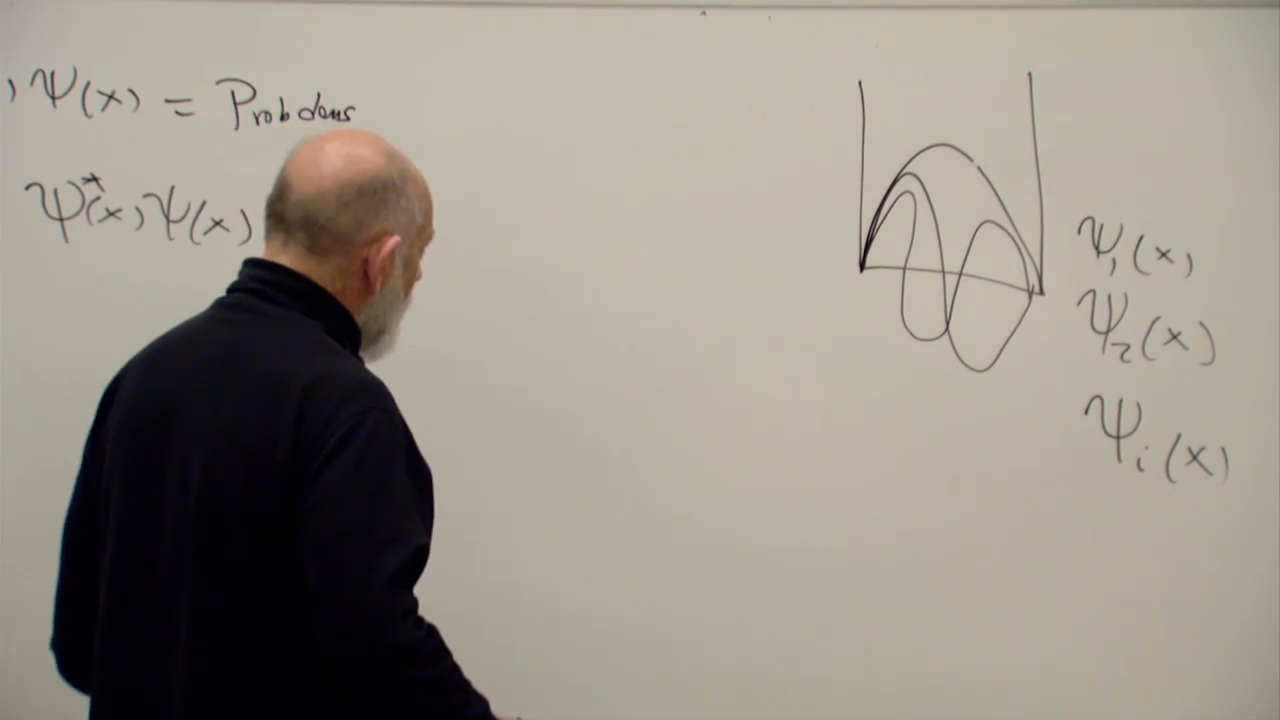
\includegraphics[width=0.94\linewidth]{lecture_07_frame_01.png}
\caption{أنماط الصندوق على لوحة المحاضرة. والآثار المتبقية في اليسار هي كثافة بورن وتطبيع الجسيم الواحد؛ أما البئر في اليمين فتُظهر \(\psi_1(x)\) و\(\psi_2(x)\) والوسم العام \(\psi_i(x)\).}
\lectureframe{00:08:25}
\end{figure}

يمكن فصل بنية الأنماط نفسها عن الحجب الموجود على اللوح أثناء الشرح:
\begin{figure}[htbp]
\centering
\begin{tikzpicture}[x=1cm,y=1cm]
  \draw[thick] (0,0) -- (0,4.0);
  \draw[thick] (7,0) -- (7,4.0);
  \draw[gray!55] (0,2.85) -- (7,2.85);
  \draw[gray!55] (0,1.35) -- (7,1.35);
  \draw[blue!75!black,thick,domain=0:7,samples=120]
    plot (\x,{2.85+0.62*sin(180*\x/7)});
  \draw[teal!70!black,thick,domain=0:7,samples=120]
    plot (\x,{1.35+0.55*sin(360*\x/7)});
  \node[right] at (7.15,3.20) {$\psi_1(x)$};
  \node[right] at (7.15,1.70) {$\psi_2(x)$};
  \node at (3.5,0.38) {$\vdots\quad\psi_i(x)$};
\end{tikzpicture}
\caption{إعادة بناء نظيفة للرسم التخطيطي الكيفي للصندوق. والإزاحات العمودية لا تفعل إلا فصل الدالتين الموجيتين لأغراض العرض.}
\end{figure}

التعامد المعياري هو
\begin{equation}
\int dx\,\psi_i^*(x)\psi_j(x)=\delta_{ij}.
\label{eq:l07-orthonormality}
\end{equation}
فإذا كان \(i=j\) كانت الحالة مطبَّعة ويكون التكامل واحدًا. وإذا كان \(i\ne j\) كانت الحالتان متعامدتين وينعدم التكامل.

والاكتمال هو العبارة التي لا تقل أهمية
\begin{equation}
\sum_i |i\rangle\langle i|=\mathbf 1.
\label{eq:l07-resolution}
\end{equation}
فكل \(|i\rangle\langle i|\) يُسقِط على اتجاه أساس واحد؛ ومجموعها على الأساس التام هو مؤثر الوحدة. وتأثيره في متجه اعتباطي لا يفعل سوى تحليل ذلك المتجه إلى مركباته ثم إعادة تركيبه.

الآن أدرج المعادلة~\eqref{eq:l07-resolution} بين حالتي موضع:
\begin{align}
\langle y|x\rangle
&=\sum_i\langle y|i\rangle\langle i|x\rangle \\
&=\sum_i\psi_i(y)\psi_i^*(x) \\
&=\delta(y-x).
\label{eq:l07-position-completeness}
\end{align}
وتوضع النجمة على العامل الذي يكون ترتيب البرا-كِت فيه \(\langle i|x\rangle\). وعكس \(x\) و\(y\) يعطي الصورة المكافئة المرافقة عقديًا. ومن ثم يزوّد كل أساس تام متعامد معياريًا تمثيلًا لدالة دلتا. فالجيوب، وجيوب التمام، والدوال الموجية للمذبذب، والدوال الذاتية للطاقة تؤدي العمل نفسه.

\begin{classroomqa}
\lecturetimestamp{00:13:43}
\audiencequestion{هل ينبغي أن تحمل الدالة الموجية الثانية في مجموع الاكتمال المرافق العقدي؟}
\lecturerresponse{نعم. مع الترتيب \(\langle y|i\rangle\langle i|x\rangle\) تكون العوامل \(\psi_i(y)\psi_i^*(x)\). وإبقاء ترتيب البرا-كِت ظاهرًا يمنع تخمين موضع النجمة أو وضعها في غير موضعها.}
\end{classroomqa}

هذه هي رياضيات الجسيم الواحد التي سنحتاج إليها. والآن نغيّر فضاء الحالات.

\section{فضاء فوك بوصفه فضاء الحالات الأكبر}

بالنسبة إلى العديد من الجسيمات المتماثلة، هناك أساس مناسب يسجّل كم جسيمًا يشغل كل نمط أحادي الجسيم:
\begin{equation}
|n_1,n_2,n_3,\ldots\rangle.
\label{eq:l07-fock-basis}
\end{equation}
والعدد الصحيح \(n_i\) هو عدد الإشغال للنمط \(i\). وهذا الكِت ليس حالةَ جسيم واحد مكتوبةً بترميز منمق. إنه ينتمي إلى فضاء هيلبرت أكبر يحتوي على قطاع انعدام الجسيمات، وكل حالة ذات جسيم واحد، وكل حالة ذات جسيمين، وهكذا. ويُسمّى ذلك الفضاء الأكبر فضاء فوك.

ولتغيير الإشغالات، ندخل لكل نمط مؤثر خلق ومؤثر إفناء،
\begin{equation}
a_i^\dagger,\qquad a_i.
\end{equation}
فالأول يضيف جسيمًا واحدًا إلى النمط \(i\)، بينما يزيل الثاني جسيمًا واحدًا. وفي هذه المرحلة، ليست لغة المذبذب التوافقي إلا أداةً تنظيمية: ليس من الضروري أن يكون هناك نابض حقيقي يهتز. وتعطينا جبرية المذبذب بالضبط الآلية اللازمة لرفع أعداد الإشغال وخفضها.

ومؤثر عدد الإشغال للنمط هو
\begin{equation}
\begin{aligned}
N_i&=a_i^\dagger a_i,\\
N_i|n_1,\ldots,n_i,\ldots\rangle
&=n_i|n_1,\ldots,n_i,\ldots\rangle.
\end{aligned}
\end{equation}
والخلاء هو
\begin{equation}
|0\rangle\equiv|0,0,0,\ldots\rangle,
\qquad
a_i|0\rangle=0
\quad\text{for every }i.
\label{eq:l07-vacuum}
\end{equation}
ولذلك فإن حالة الجسيم الواحد في النمط \(i\) هي
\begin{equation}
|i\rangle=a_i^\dagger|0\rangle.
\label{eq:l07-mode-created}
\end{equation}
ويمكن الآن قراءة الرمز نفسه \(|i\rangle\) إما على أنه متجه أساس للجسيم الواحد، أو على أنه ذلك المتجه مُدرَجًا في قطاع الجسيم الواحد من فضاء فوك. وهذا التضمين هو ~\eqref{eq:l07-mode-created}؛ ويبيّن السياق المحيط أيَّ الفضاءين هو موضع النقاش.

\section{تجميع الأنماط في حقل}

عرّف حقلي الإفناء والخلق كما يلي
\begin{equation}
\Psi(x)=\sum_i \psi_i(x)a_i,
\qquad
\Psi^\dagger(x)=\sum_i \psi_i^*(x)a_i^\dagger.
\label{eq:l07-field-expansion}
\end{equation}
إن الحرف الكبير مهم. فالدوال الصغيرة \(\psi_i(x)\) أعداد عقدية؛ أما \(\Psi(x)\) الكبيرة فهي مؤثر على فضاء فوك. وعند كل نقطة مكانية \(x\)، تعطي المعادلة~\eqref{eq:l07-field-expansion} تركيبًا خطيًا مختلفًا من مؤثرات الأنماط. وهذا هو معنى أن تكون لدينا دالة في الموضع ذات قيم مؤثرية.

بالنسبة إلى الجسيمات الحرة، قد تكون دوال الأنماط أمواجًا مستوية \(e^{ikx}\). وعندئذ تكون المعادلة~\eqref{eq:l07-field-expansion} توسعًا فورييه، إلا أن معاملات فورييه فيها مؤثرات لا أعداد. ويُطلق الاصطلاح القديم على الأعداد العقدية العادية اسم أعداد \(c\)، وعلى المؤثرات الكمومية اسم أعداد \(q\). ودوال الأنماط من النوع \(c\) وتتبادل مع كل شيء؛ أما \(a_i\) و\(a_i^\dagger\) فيحملان الطابع المؤثري.

ليس \(\Psi\) ولا \(\Psi^\dagger\) هيرميتيًا. ومرافق كل منهما هو الآخر. أما التركيبان
\begin{equation}
\Psi+\Psi^\dagger,
\qquad
i(\Psi^\dagger-\Psi)
\label{eq:l07-hermitian-combinations}
\end{equation}
فهما هيرميتيان ويمكن أن يمثلا كميات قابلة للرصد. لكن الحقول، في الوقت الراهن، تفيد أكثر بوصفها أدوات تخلق الجسيمات وتفنيها وتعدّها موضعيًا.

\begin{classroomqa}
\lecturetimestamp{00:21:05}
\audiencequestion{ما معنى أن يعتمد مؤثر على \(x\)؟}
\lecturerresponse{معناه أن كل قيمة لـ \(x\) تحدد مؤثرًا مختلفًا. فالاعتماد المكاني يكمن في دوال الأنماط العادية، بينما يؤثر كل تركيب خطي ناتج في فضاء فوك نفسه.}
\end{classroomqa}

\section{ما الذي يفعله حقل الخلق}

يصبح التعريف مفيدًا عندما نسأل عمّا يفعله. ابدأ بحالة ذاتية للموضع في قطاع الجسيم الواحد، وأدرج تحليل الوحدة:
\begin{align}
|x\rangle
&=\sum_i |i\rangle\langle i|x\rangle \\
&=\sum_i a_i^\dagger|0\rangle\,\psi_i^*(x) \\
&=\Psi^\dagger(x)|0\rangle.
\label{eq:l07-local-creation}
\end{align}
وهكذا فإن \(a_i^\dagger\) يخلق جسيمًا في النمط المحدد \(i\)، في حين أن \(\Psi^\dagger(x)\) يخلق جسيمًا متموضعًا عند \(x\). وفي أساس الموضع المثالي يكون هذا التموضع توزيعيًا؛ أما التحضير الفيزيائي فسيستخدم حزمة موجية ضيقة، لكن المعنى الجبري هو نفسه.

\begin{classroomqa}
\lecturetimestamp{00:24:48}
\audiencequestion{هل \(\sum_i|i\rangle\langle i|\) إسقاط؟}
\lecturerresponse{كل حد هو إسقاط على حالة أساس واحدة. أما المجموع الكامل فهو مؤثر الوحدة نفسه ويُسمّى تحليل الوحدة. وإدراجه لا يغيّر أي حالة، لكنه يُظهر مركبات الحالة في الأساس المختار.}
\end{classroomqa}

تمثّل المعادلة~\eqref{eq:l07-local-creation} أول تفسير مباشر للحقل من حيث الجسيمات. فلم نكتفِ بمجرد إلحاق وسم مكاني بمؤثر مجرد. بل بنينا العملية التي تُنشئ جسيمًا عند تلك النقطة المكانية.

\begin{classroomqa}
\lecturetimestamp{00:28:20}
\audiencequestion{هل ينبغي تمييز حقل الخلق في فضاء الموضع بنجمة أم بخنجر؟}
\lecturerresponse{استعمل خنجرًا للمرافق المؤثري. أما النجوم فتدل على المرافق العقدي للدوال الموجية العادية \(\psi_i(x)\)؛ والخناجر توضع على \(a_i^\dagger\) و\(\Psi^\dagger(x)\).}
\end{classroomqa}

\begin{classroomqa}
\lecturetimestamp{00:28:36}
\audiencequestion{هل يمكن تمرير مؤثرات الخلق عبر دوال الموجة في توسيع الأنماط؟}
\lecturerresponse{نعم. إن \(\psi_i(x)\) هي أعداد \(c\)، ولذلك فهي تتبادل مع كل مؤثر. ولا يلزم الحذر إلا عند تغيير ترتيب مؤثرات غير متبادلة مثل \(a_i\) و\(a_j^\dagger\).}
\end{classroomqa}

\section{من كثافة الاحتمال إلى كثافة الجسيمات}

لنتعامل الآن مع الحقل. وأول تعبير طبيعي هو
\begin{equation}
\int dx\,\Psi^\dagger(x)\Psi(x).
\end{equation}
وهو يشبه تكامل التطبيع للجسيم الواحد، لكن عوامله أصبحت الآن مؤثرات. أدرج توسعات الأنماط من دون تغيير ترتيبها:
\begin{align}
\int dx\,\Psi^\dagger(x)\Psi(x)
&=\int dx
\left(\sum_i a_i^\dagger\psi_i^*(x)\right)\\
&\qquad\times\left(\sum_j a_j\psi_j(x)\right) \\
&=\sum_{i,j}a_i^\dagger a_j
\int dx\,\psi_i^*(x)\psi_j(x) \\
&=\sum_{i,j}a_i^\dagger a_j\,\delta_{ij} \\
&=\sum_i a_i^\dagger a_i.
\label{eq:l07-number-derivation}
\end{align}
ومن ثم فإن مؤثر العدد الكلي هو
\begin{equation}
N=\sum_i N_i
=\int dx\,\Psi^\dagger(x)\Psi(x).
\label{eq:l07-total-number}
\end{equation}
في الحالات التي نناقشها، تكون إشغالات الإثارات ذات الطاقة المنتهية متضائلة عند طاقات الأنماط العالية بما يكفي، ولذلك يكون هذا المجموع منتهيًا عادةً رغم أن قائمة الأنماط الممكنة لا نهائية.

الكمية تحت إشارة التكامل هي مؤثر كثافة الجسيمات الموضعي:
\begin{equation}
n(x)=\Psi^\dagger(x)\Psi(x).
\label{eq:l07-density}
\end{equation}
وبالمعنى الدقيق، لا تُقاس الكثافة عند نقطة رياضية. بل لمنطقة صغيرة \(R\)، يُقاس
\begin{equation}
N_R=\int_R dx\,n(x),
\label{eq:l07-regional-number}
\end{equation}
أي عدد الجسيمات في تلك المنطقة. ومثل أي مرصود كمومي، ليس من الضروري أن تكون لـ \(N_R\) قيمة محددة في حالة اعتباطية. وقد تعطي عمليات التحضير المتكررة نتائج مختلفة.

\begin{classroomqa}
\lecturetimestamp{00:36:27}
\audiencequestion{هل \(\Psi^\dagger(x)\Psi(x)\) هي كثافة الاحتمال متعددة الجسيمات؟}
\lecturerresponse{معناها المباشر هو كثافة الجسيمات. أما السعة الاحتمالية متعددة الجسيمات فتعتمد عمومًا على جميع إحداثيات الجسيمات. وعلى النقيض من ذلك، فإن المقدار الثنائي الخطي الموضعي يعدّ الجسيمات في منطقة صغيرة عند تكامله على تلك المنطقة.}
\end{classroomqa}

\begin{classroomqa}
\lecturetimestamp{00:38:28}
\audiencequestion{هل يؤثر المؤثران \(a_i\) و\(a_i^\dagger\) في متجهات الحالة فقط، لا في دوال الموجة أحادية الجسيم؟}
\lecturerresponse{نعم. فهما يؤثران في حالات فضاء فوك مثل \(|n_1,n_2,\ldots\rangle\). أما دوال الأنماط أحادية الجسيم التي تضربهما فهي أعداد عادية، وليست هي الأشياء التي تعمل عليها مؤثرات السلم هذه.}
\end{classroomqa}

تشكل كيتات الإشغال أساسًا، لكنها ليست الحالة الأكثر عمومية. ويمكن تراكبها، بما في ذلك تراكيب خطية يُوزَّع فيها العدد الكلي نفسه على الأنماط بطرق مختلفة. وبالنسبة إلى الأنواع المتعادلة مثل الفوتونات، يمكن أيضًا تراكب أعداد كلية مختلفة من الجسيمات. ويحتفظ المؤثر في المعادلة~\eqref{eq:l07-regional-number} بالمعنى التشغيلي نفسه في كل حالة من هذا النوع.

\begin{classroomqa}
\lecturetimestamp{00:40:01}
\audiencequestion{إذا قُسمت كثافة الجسيمات على العدد الكلي، فهل تصبح كثافة الاحتمال لإيجاد جسيم عند \(x\)؟}
\lecturerresponse{في حالة يكون فيها \(N\) ثابتًا ويكون عدد الجسيمات كبيرًا، يكون \(N_R/N\) تواترًا نسبيًا ويوافق عادةً احتمال الجسيم الواحد على نحو جيد جدًا. لكنه ليس هويةً مؤثرية تُساوي بين ناتج قياس واحتمال. فالعدّ المقاس يتقلب، وعادةً بمقدار من رتبة \(\sqrt N\) في صورة الجسيمات المستقلة، ويمكن لتكرار استثنائي واحد أن يختلف كثيرًا عن الاحتمال رغم أن مثل هذا التكرار غير مرجح.}
\end{classroomqa}

\begin{classroomqa}
\lecturetimestamp{00:42:25}
\audiencequestion{ماذا يحدث لانحفاظ الشحنة في تراكب بين حالة إلكترون واحد وحالة بلا إلكترونات؟}
\lecturerresponse{هذا ليس نوع التراكب المستخدم في قطاع مغلق ذي شحنة كهربائية كلية ثابتة. ويمكن تراكب توزيعات مختلفة لها الشحنة الكلية نفسها. ولا تحمل الفوتونات شحنة كهربائية، لذا فإن قطاعات أعداد الفوتونات المختلفة لا تثير مثل هذه المشكلة. ويمكن أيضًا أن يتغير عدد الإلكترونات والبوزيترونات معًا بينما تبقى الشحنة الصافية ثابتة.}
\end{classroomqa}

\section{طاقة الجسيمات المستقلة}

المرصود التالي هو الطاقة. ولنقصر الحديث أولًا على جسيمات لا تتفاعل فيما بينها. وغالبًا ما يكون هذا تقريبًا جيدًا في منظومة مخلخلة. وحتى الفوتونات تتفاعل من حيث المبدأ عبر عمليات من رتبة أعلى، لكن الإشعاع المخبري العادي مخلخل بما يكفي بحيث يكون وصف الجسيمات المستقلة ممتازًا.

لتدل \(\omega_i\) على طاقة جسيم واحد في النمط \(i\)، مع \(\hbar=1\). والمقصود بالنمط هو حالة واحدة لجسيم واحد. وعندئذ يكون الهاملتوني الكلي
\begin{equation}
H=\sum_i\omega_i N_i
=\sum_i\omega_i a_i^\dagger a_i.
\label{eq:l07-mode-hamiltonian}
\end{equation}
ويسهم كل نمط مشغول بطاقة الجسيم الواحد الخاصة به مرةً واحدة عن كل جسيم.

\begin{classroomqa}
\lecturetimestamp{00:48:16}
\audiencequestion{هل \(\omega_i\) دالة في الموضع؟}
\lecturerresponse{لا. إنها القيمة الذاتية للطاقة المرتبطة بالنمط \(i\). أما الدالة \(\psi_i(x)\) فتعتمد على الموضع؛ و\(\omega_i\) يعتمد على مستوى الطاقة الذي جرى اختياره.}
\end{classroomqa}

تتحدد القيم \(\omega_i\) بمعادلة شرودنغر المستقلة عن الزمن لجسيم واحد. عرّف
\begin{equation}
h=-\frac{\nabla^2}{2m}+V(x).
\label{eq:l07-one-particle-h}
\end{equation}
وعندئذٍ
\begin{equation}
h\psi_i(x)=\omega_i\psi_i(x).
\label{eq:l07-schrodinger-eigenvalue}
\end{equation}
في بعد واحد يكون مؤثر الزخم هو \(p=-i\partial_x\)، ويصبح \(p^2/(2m)\) هو \(-\partial_x^2/(2m)\). وفي ثلاثة أبعاد تتجمع المشتقات الثانية الثلاث في \(-\nabla^2/(2m)\).

\begin{figure}[htbp]
\centering
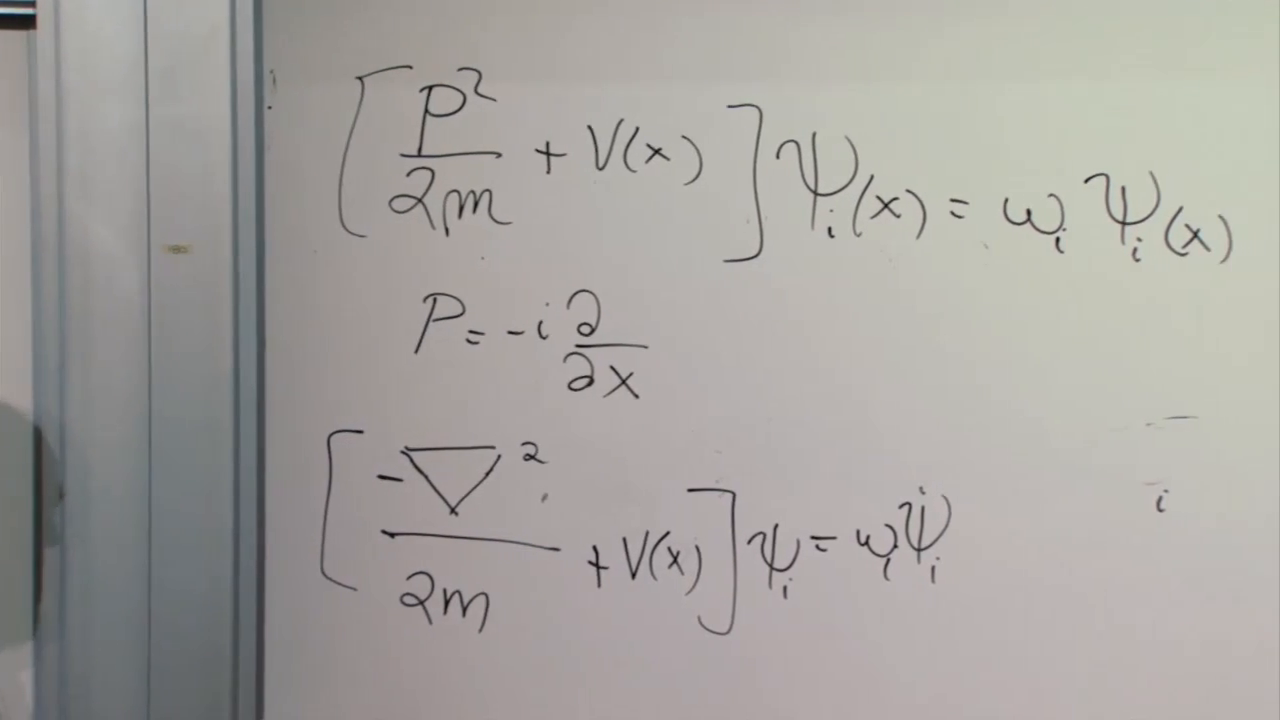
\includegraphics[width=0.94\linewidth]{lecture_07_frame_02.png}
\caption{الانتقال على اللوح من \(p^2/(2m)+V(x)\) إلى الصيغة التفاضلية لمعادلة القيم الذاتية لشرودنغر لجسيم واحد. والمعادلة~\eqref{eq:l07-schrodinger-eigenvalue} هي إعادة بنائها المنقحة.}
\lectureframe{00:54:10}
\end{figure}

بالنسبة إلى دالة موجة مطبَّعة اعتباطية لجسيم واحد، فإن قيمة التوقع المألوفة هي
\begin{equation}
\langle h\rangle_\psi
=\int dx\,\psi^*(x)h\psi(x).
\label{eq:l07-one-particle-energy-expectation}
\end{equation}
وتُستوحى الصيغة عديدة الجسيمات من استبدال دالة الموجة المكتوبة بحرف صغير بالحقل ذي القيم المؤثرية. وهذا ليس برهانًا بعد؛ بل هو التخمين الذي نختبر الآن صحته:
\begin{equation}
H=\int dx\,\Psi^\dagger(x)h\Psi(x).
\label{eq:l07-field-hamiltonian}
\end{equation}

\section{إعطاء الجواب أولًا ثم إثباته}

أدرِج المعادلة~\eqref{eq:l07-field-expansion} في الهاملتوني المقترح:
\begin{align}
\int dx\,\Psi^\dagger h\Psi
&=\int dx
\left(\sum_i a_i^\dagger\psi_i^*(x)\right)
h\left(\sum_j a_j\psi_j(x)\right) \\
&=\sum_{i,j}a_i^\dagger a_j
\int dx\,\psi_i^*(x)h\psi_j(x).
\label{eq:l07-h-expanded}
\end{align}
يؤثر المؤثر التفاضلي \(h\) في دالة الموجة \(\psi_j(x)\) المعتمدة على \(x\)، لا في مؤثر النمط \(a_j\). وبحسب معادلة شرودنغر،
\begin{equation}
h\psi_j(x)=\omega_j\psi_j(x).
\end{equation}
ومن ثم،
\begin{align}
\int dx\,\Psi^\dagger h\Psi
&=\sum_{i,j}a_i^\dagger a_j\omega_j
\int dx\,\psi_i^*(x)\psi_j(x) \\
&=\sum_{i,j}a_i^\dagger a_j\omega_j\delta_{ij} \\
&=\sum_j\omega_j a_j^\dagger a_j.
\label{eq:l07-h-proof}
\end{align}
وهذا يطابق تمامًا المعادلة~\eqref{eq:l07-mode-hamiltonian}. فالتعبير الحقلي الموضعي ومجموع جميع طاقات الجسيمات هما المؤثر نفسه.

\begin{figure}[htbp]
\centering
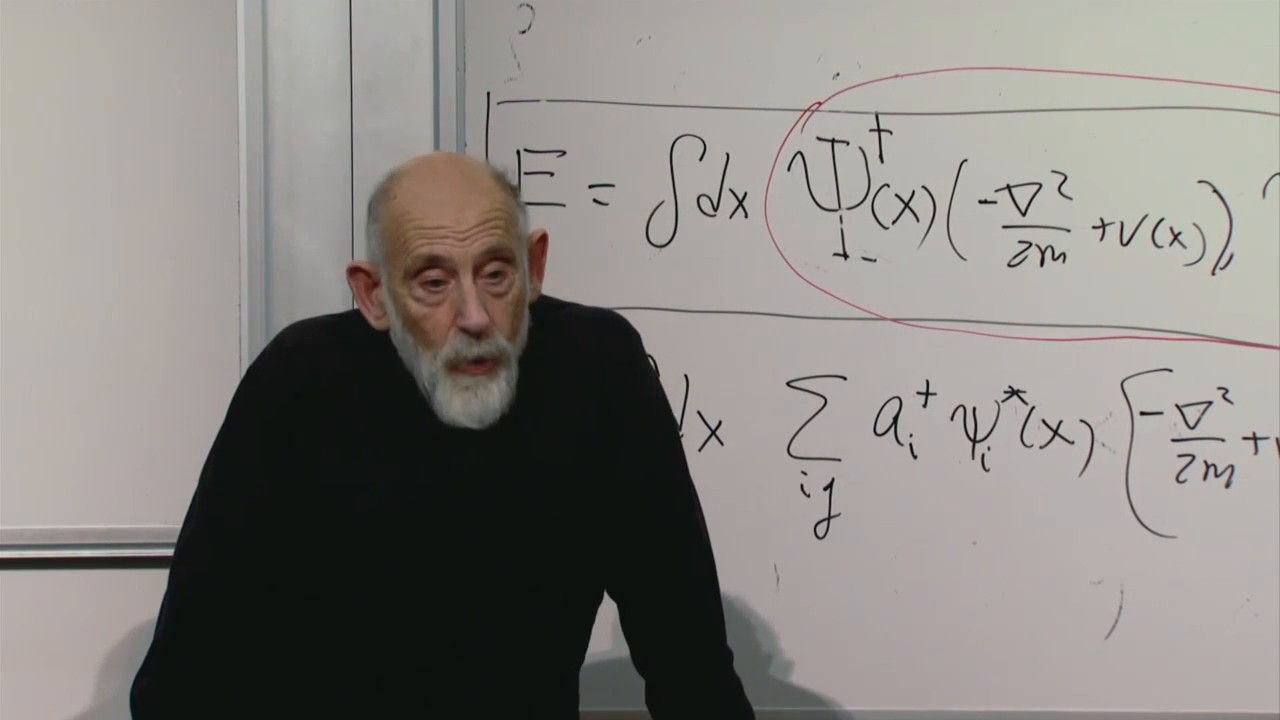
\includegraphics[width=0.94\linewidth]{lecture_07_frame_03.png}
\caption{الهاملتوني الحقلي الذي جرى التأكيد عليه على اللوح، ويبدأ أسفله البرهان بتوسيع الأنماط. وقد أُبقيت الصورة الحية بوصفها شاهدًا؛ وتستعيد المعادلات~\eqref{eq:l07-field-hamiltonian}--\eqref{eq:l07-h-proof} الجبر الكامل.}
\lectureframe{01:05:34}
\end{figure}

لم يُبدَّل ترتيب أي مؤثر خلق مع مؤثر إفناء في هذا الاشتقاق. وقد حُوفظ على ترتيب \(a_i^\dagger a_j\) من البداية إلى النهاية. والأشياء الوحيدة التي نُقلت بحرية هي دوال الموجة من نوع \(c\) وقيمها الذاتية.

\section{لماذا يُعد هذا حقلًا}

لماذا نسمّي \(\Psi(x)\) حقلًا؟ لأنه كمية ذات قيم مؤثرية معرّفة عند كل نقطة من الفضاء، ولأن التراكيب الهرميتية أو المقادير الثنائية الخطية المبنية منه هي مرصودات موضعية. وتمثل الكثافة \(n(x)\) وتعبير الطاقة الموضعي أدناه مثالين. ولا يوجد اختبار رياضي إضافي مخبوء وراء هذه الكلمة.

هذا الحقل ليس الحقل الكهرومغناطيسي. فهو يصف أي نوع غير نسبي تُستمد منه أنماط الجسيم الواحد والهاملتوني \(p^2/(2m)+V\): مثل الذرات البطيئة الحركة، أو النيوترونات، أو البروتونات، أو الإلكترونات. وهذه الجسيمات هي كمّات حقلها الموافق، بالمعنى البنيوي نفسه الذي تكون فيه الفوتونات كمّات الحقل الكهرومغناطيسي.

\begin{classroomqa}
\lecturetimestamp{01:02:45}
\audiencequestion{أين، عند الانتقال من المنظومة عديدة الجسيمات إلى الصيغة أعلاه، دخل الحقل؟}
\lecturerresponse{لقد دخل في المعادلة~\eqref{eq:l07-field-expansion}: فـ \(\Psi(x)\) مؤثر عند كل نقطة مكانية. وتبيّن الاشتقاقات اللاحقة أن جداءاته الموضعية تقيس كثافتي الجسيمات والطاقة. والاعتماد على الموضع مع المحتوى المؤثري هو بالضبط البنية الحقلية التي يجري بناؤها.}
\end{classroomqa}

\section{كثافة الطاقة الموضعية}

تكتب المعادلة~\eqref{eq:l07-field-hamiltonian} الطاقة الكلية على أنها تكامل على الفضاء،
\begin{equation}
\begin{aligned}
H&=\int dx\,\mathcal H(x),\\
\mathcal H(x)
&=-\frac{1}{2m}\Psi^\dagger(x)\nabla^2\Psi(x)\\
&\quad+V(x)\Psi^\dagger(x)\Psi(x).
\end{aligned}
\label{eq:l07-hamiltonian-density}
\end{equation}
والكمية تحت إشارة التكامل هي كثافة طاقة موضعية طبيعية لهذا الهاملتوني. وصيغتها الموضعية غير وحيدة. فعلى سبيل المثال، يستبدل التكامل بالأجزاء الحد الحركي بـ
\begin{equation}
\mathcal H_{\rm kin}(x)
=\frac{1}{2m}\nabla\Psi^\dagger(x)\mathbin{\cdot}\nabla\Psi(x)
\label{eq:l07-kinetic-density}
\end{equation}
حتى حدّ حدودي. ويعطي التعبيران الهاملتوني الكلي نفسه تحت الشروط الحدية المعتادة. وهذا هو الالتباس الصغير المذكور في المحاضرة.

\begin{classroomqa}
\lecturetimestamp{01:05:57}
\audiencequestion{هل يجب تكامل كثافة الطاقة على الفضاء كله؟}
\lecturerresponse{إن التكامل على الفضاء كله يعطي الطاقة الكلية. أما التكامل على منطقة أصغر فيعطي الطاقة المسندة إلى تلك المنطقة، مع مراعاة الالتباس المعتاد في اختيار كثافة موضعية يكون تكاملها الكامل هو الهاملتوني نفسه.}
\end{classroomqa}

\begin{classroomqa}
\lecturetimestamp{01:06:25}
\audiencequestion{كيف يختلف \(N_i\) ذو الحرف الكبير في صيغة الطاقة عن \(n_i\) ذي الحرف الصغير؟}
\lecturerresponse{\(N_i=a_i^\dagger a_i\) مؤثر. والعدد الصحيح \(n_i\) هو إحدى قيمه الذاتية على حالة عدد الإشغال. تؤثر المؤثرات في الحالات؛ أما قيمها الذاتية فهي أعداد عادية.}
\end{classroomqa}

\begin{classroomqa}
\lecturetimestamp{01:06:46}
\audiencequestion{هل يمكن كتابة هاملتوني الحقل نفسه على صورة برا أو كيت في ترميز ديراك؟}
\lecturerresponse{لا. تدل البرا والكيت على متجهات الحالة ومزدوجاتها. الحقل والهاملتوني مؤثران يؤثران في تلك الحالات. وقيمة التوقع مثل \(\langle\Phi|H|\Phi\rangle\) تستخدم كلا النوعين من الكائنات ولا يجوز اعتبارهما شيئًا واحدًا.}
\end{classroomqa}

\section{استعادة الجسيم الواحد والاقتراب من حقل كلاسيكي}

تتضمن الصياغة الموسعة ميكانيكا الكم العادية لجسيم واحد. نقصر فضاء فوك على الحالات التي تحقق
\begin{equation}
N|\Phi\rangle=|\Phi\rangle.
\end{equation}
ضمن ذلك القطاع، يعيد البناء الحقلي إنتاج كل حالة لجسيم واحد وكل تنبؤ خاص بجسيم واحد. لم نستبدل النظرية القديمة؛ بل أدرجناها في فضاء يستطيع أيضًا وصف انعدام الجسيمات، أو جسيمين، أو عدد اعتباطي من الجسيمات.

وعلى الطرف الآخر، يمكن لنمط يشغله عدد كبير جدًا من البوزونات أن يسلك تقريبًا كموجة كلاسيكية. في حالات متماسكة أو شبه كلاسيكية مناسبة، فإن قيمة التوقع
\begin{equation}
\Phi_{\rm cl}(x,t)=\langle\Psi(x,t)\rangle
\end{equation}
تطيع المعادلة ذات المظهر الكلاسيكي
\begin{equation}
i\partial_t\Phi_{\rm cl}(x,t)
=\left(-\frac{\nabla^2}{2m}+V(x)\right)\Phi_{\rm cl}(x,t)
\label{eq:l07-classical-schrodinger}
\end{equation}
في النظرية الحرة غير النسبية. تذكر المحاضرة هذه الصلة بدلًا من اشتقاقها. وهي الجسر بين مجموعة من الكوانتا وحقل موجي: فالإشغالات الكبيرة تقمع التقلبات النسبية وتجعل قيم التوقع المناسبة تسلك سلوكًا كلاسيكيًا.

ولذلك فهذه الصياغة تؤدي دور التنظيم الحسابي كما تؤدي دور الفيزياء. فهي تنظم جميع قطاعات عدد الجسيمات، لكنها تلتقط أيضًا التداخل والتشابك ونشوء الموجات الكلاسيكية من الجسيمات الكمومية.

\begin{classroomqa}
\lecturetimestamp{01:10:43}
\audiencequestion{لماذا يمكن التعامل مع مؤثرات الخلق والفناء داخل التكامل تقريبًا كما لو كانت أعدادًا عادية؟}
\lecturerresponse{لأنه لم يُبدَّل موضع بعضها مع بعض أصلًا. دوال الأنماط العادية تبدّل معها، والمشتقات تؤثر في تلك الدوال فقط. أما تمرير مؤثر فناء عبر مؤثر خلق فيستلزم المبدل وقد يضيف حدًا؛ ولا شيء في البرهان يقوم بهذه الخطوة.}
\end{classroomqa}

\section{استطراد في ترميز ديراك}

بعض هذا الالتباس تاريخي. فدالة الموجة لجسيم واحد تحقق معادلة موجية وتبدو ظاهريًا كحقل كلاسيكي، ومع ذلك فهي أيضًا سعة احتمال. وكان على نظرية الكم المبكرة أن تفصل بين هذين الدورين ثم تشرح كيف تتكون الحقول الموجية القابلة للقياس فعلًا، مثل الكهرومغناطيسية، من كوانتا. ويحل فضاء فوك والحقول ذات القيم المؤثرية هذا التعارض الظاهري.

يجعل ترميز ديراك هذا الفصل موجزًا على نحو غير مألوف. فالكيت ينتمي إلى فضاء متجهي، والبرا إلى فضائه المزدوج، وتجاورهما يشكل جداءً داخليًا. وعندئذ تكاد الصيغة
\begin{equation}
\sum_i|i\rangle\langle i|=\mathbf 1
\end{equation}
تشرح نفسها بنفسها. وتوضح المحاضرة ذلك بحكاية من تدريس ميكانيكا الكم لعلماء الرياضيات: فقد كان المحتوى الرياضي مألوفًا من قبل، لكن الترميز جعل التلاعبات الروتينية شديدة الوضوح إلى درجة أن البنية بدت جديدة. وليست الفكرة أن أحد التخصصين كان يفتقر إلى المفهوم. بل إن ترميزًا حسن الاختيار يمكن أن يجعل العمليات المسموح بها عسيرة الالتباس.

لهذا الدرس أهمية هنا. توجد الآن عدة مؤثرات متميزة:
\begin{itemize}
\item \(h\) يؤثر في دوال الموجة لجسيم واحد بوصفه مؤثرًا تفاضليًا؛
\item \(a_i\) و\(a_i^\dagger\) يعملان على حالات أعداد الإشغال في فضاء فوك؛
\item \(\Psi(x)\) و\(\Psi^\dagger(x)\) و\(N\) و\(H\) تعمل أيضًا على فضاء فوك.
\end{itemize}
يربط التوسع في المعادلة~\eqref{eq:l07-field-expansion} بين السياقين الأولين من غير أن يدمجهما.

\begin{classroomqa}
\lecturetimestamp{01:18:16}
\audiencequestion{هل الحقول مجرد صياغة لوصف مجموعات من الجسيمات؟}
\lecturerresponse{إنها صياغة، لكنها ليست صياغة فارغة. يمكن قياس مراصدها الموضعية، والجسيمات فيها جسيمات كمومية لها تداخل وتشابك، لا حبيبات كلاسيكية. ومؤثرات الحقل تشفِّر بدقة تلك الخواص الجمعية القابلة للقياس.}
\end{classroomqa}

\section{تنبيه متعلق بالنسبية واستطراد كهرومغناطيسي}

البناء حتى الآن غير نسبي. يظل الزخم وسمًا جيدًا للجسيم في الفيزياء النسبية، لكن موضع الجسيم المحدد بحدة مسألة أدق بكثير. وبناءً على ذلك، فإن كثافة عدد الفوتونات الموضعية ليست عمومًا مقدارًا واضح التعريف بقدر \(n(x)\) في النظرية غير النسبية. وتبقى كثافة الطاقة محددة تحديدًا جيدًا، وهي المرصود الموضعي الأكثر أمانًا.

تقدم المحاضرة تشبيهًا كهرومغناطيسيًا مفيدًا، واسترشاديًا على نحو صريح. نجمع المجالين الكهربائي والمغناطيسي في المتجه المركب
\begin{equation}
\mathbf F=\mathbf E+i\mathbf B,
\qquad
\mathbf F^*=\mathbf E-i\mathbf B.
\label{eq:l07-riemann-silberstein}
\end{equation}
وعندئذ
\begin{equation}
\mathbf F^*\mathbin{\cdot}\mathbf F
=\mathbf E^2+\mathbf B^2,
\label{eq:l07-em-density}
\end{equation}
وهو يتناسب مع كثافة الطاقة الكهرومغناطيسية في الوحدات المتعارف عليها. وهذا ليس حرفيًا كثافة احتمال للفوتون. والأفضل أن يُنظر إليه بوصفه متغيرًا حقليًا مضغوطًا يقيس مربع معياره كثافة الطاقة، أو، على نحو غير رسمي، بوصفه كثافة فوتونات موزونة بطاقة الفوتون.

\begin{classroomqa}
\lecturetimestamp{01:19:10}
\audiencequestion{هل يمكن مطابقة كثافة الفوتونات مع شدة المجال الكهربائي؟}
\lecturerresponse{فقط على نحو نوعي ومع الحذر. بالنسبة إلى الفوتونات النسبية، ليس عدد الجسيمات الموضعي هو المفهوم المفضل. والعبارة الموثوقة هي أن \(E^2+B^2\) يتناسب مع كثافة الطاقة، وأن التركيب المركب \(\mathbf E+i\mathbf B\) يصوغ معادلات ماكسويل في صورة شبيهة بشرودنغر.}
\end{classroomqa}

\begin{classroomqa}
\lecturetimestamp{01:20:09}
\audiencequestion{لماذا يمكن لجسيم نسبي أن يملك زخمًا محددًا بينما يكون الموضع إشكاليًا؟}
\lecturerresponse{لأن الزخم يشكّل وسمًا واضحًا لتمثيلات الجسيم الواحد النسبية، في حين أن التوضع الصارم يتعارض مع خلق الجسيمات ومع الوصف الحقلي النسبي. لا تطور هذه المحاضرة تلك النظرية؛ وإنما يشير هذا التحذير إلى حد تفسير الكثافة غير النسبي الحالي.}
\end{classroomqa}

\section{الترتيب وثابت الحالة القاعية}

لا يمكن تغيير ترتيب المؤثرات على نحو اعتباطي. بالنسبة إلى الأنماط البوزونية،
\begin{equation}
a_i a_i^\dagger=a_i^\dagger a_i+1.
\end{equation}
وبناءً على ذلك، فإن استبدال الترتيب العادي \(\Psi^\dagger h\Psi\) بالترتيب المعكوس \((h\Psi)\Psi^\dagger\)، أو إجراء هذا الاستبدال في نظيره المتكامل على الوجه الصحيح، يضيف مساهمة المبدل. وفي أساس الأنماط يكون هذا مجموعًا إضافيًا مقداره كمّ واحد من الطاقة لكل نمط. وهو ثابت الحالة القاعية أو ثابت طاقة نقطة الصفر، وفي المتصل يحتاج إلى تنظيم. لا تتوسع المحاضرة في هذه المسألة هنا؛ وإنما تنبه فقط إلى أن الترتيبين غير متساويين.

\begin{classroomqa}
\lecturetimestamp{01:22:04}
\audiencequestion{ما الذي يحدث إذا بُدِّل ترتيب \(\Psi\) و\(\Psi^\dagger\) في الهاملتوني؟}
\lecturerresponse{يجب تضمين مبادلهما. لذلك فإن عكس الترتيب يضيف مساهمة في طاقة الحالة القاعية مستقلة عن الحالة بدلًا من إعادة إنتاج التعبير نفسه. ويُبقى الهاملتوني المعروض في الترتيب العادي، \(\Psi^\dagger h\Psi\).}
\end{classroomqa}

\section{الزخم بوصفه الاختبار الأخير}

تعيد الدقائق الأخيرة عملية الترقية نفسها مرة أخرى. بالنسبة إلى جسيم واحد،
\begin{equation}
\langle p\rangle_\psi
=\int dx\,\psi^*(x)\left(-i\partial_x\right)\psi(x).
\label{eq:l07-one-particle-momentum}
\end{equation}
فإن استبدال دالة الموجة بالحقل يعطي مؤثر الزخم الكلي
\begin{equation}
P=\int dx\,\Psi^\dagger(x)\left(-i\partial_x\right)\Psi(x),
\label{eq:l07-field-momentum}
\end{equation}
أو، في ثلاثة أبعاد،
\begin{equation}
\mathbf P=\int d^3x\,\Psi^\dagger(\mathbf x)
\left(-i\boldsymbol\nabla\right)\Psi(\mathbf x).
\end{equation}
تحمل الحقول زخمًا. فالليزر ذو القدرة الكافية ينقل زخمًا إلى جدار ويؤثر بقوة؛ وفي الوصف الكمومي يكون الزخم الذي يحمله الحقل هو مجموع زخوم الفوتونات.

المعادلة~\eqref{eq:l07-field-momentum} تمثل مؤثرًا، لا قيمة توقع. وإذا أُعطيت حالة في فضاء فوك \(|\Phi\rangle\)، أمكن عندئذ حساب
\begin{equation}
\langle P\rangle_\Phi=\langle\Phi|P|\Phi\rangle.
\end{equation}
ويلزم كل من مؤثر وحالة لتكوين قيمة توقع. وإن الخلط بين المرصود ومتوسطه يمحو بالضبط التمييز الذي عملت المحاضرة على إقامته.

\begin{classroomqa}
\lecturetimestamp{01:26:02}
\audiencequestion{هل زخم الحقل المعروض هو بالفعل الزخم المتوسط؟}
\lecturerresponse{لا. إنه المؤثر الهيرميتي الذي يمثل المرصود. وبإعطاء حالة ووضع المؤثر بين براها وكيتها تُحصَل قيمة توقع؛ ومع ذلك يمكن للقياس أن يتقلب حول ذلك المتوسط.}
\end{classroomqa}

هذه هي نقطة التوقف الطبيعية. انطلاقًا من الجسيمات، شيدنا حقول خلق وفناء موضعية، واستخدمناها لعد الجسيمات، وأعدنا كتابة مجموع طاقات الجسيم الواحد وزخومه على صورة مؤثرات حقلية. والخطوة التالية ليست تغييرًا آخر في الترميز. بل هي أن نسمح لمؤثرات الحقل بأن تمثل عمليات فيزيائية: جسيمات تضمحل، وجسيمات تتبعثر، وأنواع الجسيمات تتحول بعضها إلى بعض.

\chapter{الخلط، والتذبذب، وعزوم ثنائية القطب الكهربائية، ومؤثرات الحقول}

نبدأ خارج الموضوع المعلن قليلًا، بسؤال عن النيوترينوات. توجد أدلة على أن للنيوترينوات كتلة، وأن أنواع النيوترينو تختلط. فإذا لم تكن الكتل كلها متساوية، فكيف يمكن لنوعٍ أن يتحول إلى آخر من دون انتهاك حفظ الطاقة؟

يشير هذا السؤال إلى نمط يظهر في ميكانيكا الكم كلها: فالحالات التي يُحضَّر فيها نظام أو يُكشَف فيها عنه ليست بالضرورة الحالات التي تجعل هاملتونيه قطريًا. والحالة ذات الطاقة المحددة لا تكتسب إلا طورًا. أما الحالة المُحضَّرة التي هي تراكب لعدة طاقات فتتغير لأن مركباتها تكتسب أطوارًا مختلفة. وسيحملنا هذا التمييز من بئر مزدوج إلى تذبذب النيوترينو وسبق السبين. وبعد استطراد عن عزم ثنائي القطب الكهربائي للإلكترون، سنعود إلى التكميم الثاني ونرى البنية الفورييهية نفسها للموضع--الزخم على مستوى المؤثرات.

\section{الخلط بوصفه القضية الحقيقية}

لا يلزم أن تكون جميع النيوترينوات ذات الكتلة نفسها. فالحالات الذاتية للطاقة لا تختلط بعضها ببعض؛ إذ يتطور كلٌّ منها على نحو مستقل. وما نسميه \emph{النوع}، أو النكهة، في النيوترينو يرتبط بكيفية إنتاجه وكشفه، ويمكن لحالة النكهة أن تكون تركيبًا خطيًا من الحالات الذاتية للكتلة والطاقة. وعلى نحو تخطيطي،
\begin{equation}
|\text{type}\rangle = \sum_n c_n |E_n\rangle .
\end{equation}
ومن ثم فالصياغة الصحيحة ليست أن الحالات الذاتية للطاقة تتحول بعضها إلى بعض، بل إن الحالات المسماة ``نيوترينو إلكتروني'' أو ``نيوترينو ميوني'' ليست بالضرورة، في حد ذاتها، حالاتٍ ذاتية للطاقة.

\begin{classroomqa}
\lecturetimestamp{00:00:09}
\audiencequestion{إذا كانت للنيوترينوات كتل مختلفة، فكيف يمكنها أن تختلط مع بقاء الطاقة محفوظة؟}
\lecturerresponse{الحالات الذاتية للكتلة والطاقة لا تتحول بعضها إلى بعض. وحالات نكهة الإلكترون والميون والتاو هي تراكيب خطية مختلفة من تلك الحالات الذاتية. ويتطور كل مركِّب كتلي بطوره الخاص، ويغيِّر التداخل احتمالات النكهة من غير انتهاك حفظ الطاقة.}
\end{classroomqa}

لهذه البنية أمثلة كثيرة. وأوضحها يبدأ بجسيم في بئر مزدوج متناظر.

\section{البئر المزدوج المتناظر والحالات المتموضعة التقريبية}

لننظر إلى جسيم يتحرك في كمون بئر مزدوج متناظر، بين القاعين فيه حاجز عالٍ. فإذا اعتُبر الحاجز لا نهائي الارتفاع، انفصلت البئران اليسرى واليمنى انفصالًا تامًا. وعندئذ يمكن حل البئر اليسرى كما لو أن البئر اليمنى غير موجودة، وبالمثل للبئر اليمنى. وتكون دالتا الموجة التقريبيتان للحالة القاعية عندئذ حالةً متموضعة إلى اليسار \(\psi_L\) وحالةً متموضعة إلى اليمين \(\psi_R\)، وكلتاهما بالطاقة نفسها \(E\).

في كل بئر معزول تمتلك الحالة القاعية الخواص النوعية المألوفة: فهي ملساء، ولا تحوي عقدًا، وتقع عند أخفض طاقة ممكنة تتسق مع الاحتجاز. تخيل الحاجز المركزي العالي جدارًا من الطوب. إن التعامل معه على أنه لا نهائي ليس إلا تقريبًا، لكنه يزوِّدنا بزوج مفيد من الحالات المتموضعة نبدأ منه.

\begin{figure}
\centering
\begin{adjustbox}{max width=\linewidth}
\begin{tikzpicture}[x=0.8cm,y=0.8cm]
\begin{scope}[shift={(-5.8,0)}]
\draw (-4,2.7) .. controls (-3.35,1.2) and (-2.55,-0.45) .. (-2.0,-0.72)
      .. controls (-1.35,-0.95) and (-0.7,0.65) .. (0,2.05)
      .. controls (0.7,0.65) and (1.35,-0.95) .. (2.0,-0.72)
      .. controls (2.55,-0.45) and (3.35,1.2) .. (4,2.7);
\draw[dashed] (-4,-0.10) -- (4,-0.10);
\node at (-3.55,-0.48) {$E$};
\draw[line width=0.9pt] (-4,-0.02) .. controls (-3.2,-0.02) and (-2.7,0.30) .. (-2.15,0.95)
      .. controls (-1.55,1.30) and (-1.15,0.35) .. (-0.55,-0.06)
      .. controls (0.15,-0.14) and (0.9,-0.15) .. (4,-0.15);
\node at (-2.15,1.35) {$\psi_L$};
\end{scope}
\begin{scope}[shift={(5.8,0)}]
\draw (-4,2.7) .. controls (-3.35,1.2) and (-2.55,-0.45) .. (-2.0,-0.72)
      .. controls (-1.35,-0.95) and (-0.7,0.65) .. (0,2.05)
      .. controls (0.7,0.65) and (1.35,-0.95) .. (2.0,-0.72)
      .. controls (2.55,-0.45) and (3.35,1.2) .. (4,2.7);
\draw[dashed] (-4,-0.10) -- (4,-0.10);
\node at (-3.55,-0.48) {$E$};
\draw[line width=0.9pt] (-4,-0.02) .. controls (-3.2,-0.01) and (-2.7,0.30) .. (-2.15,0.95)
      .. controls (-1.6,1.28) and (-1.1,0.25) .. (-0.30,-0.08)
      .. controls (0.35,-0.12) and (0.85,-0.12) .. (1.35,0.35)
      .. controls (1.9,0.88) and (2.35,1.15) .. (2.85,0.55)
      .. controls (3.2,0.05) and (3.55,-0.12) .. (4,-0.15);
\end{scope}
\end{tikzpicture}
\end{adjustbox}
\caption{إعادة رسم نظيفة لرسومات اللوح الافتتاحية. على اليسار توجد الحالة التجريبية أحادية الجانب \(\psi_L\)، الناتجة عن افتراض أن الحاجز لا نهائي فعليًا. وعلى اليمين مُدَّت دالة الموجة نفسها على نحو متناظر عبر الحاجز، موضحةً التسرب الصغير لكنه غير المنعدم الذي يُنتج في النهاية الحالة القاعية الزوجية الحقيقية.}
\end{figure}

لكن الحاجز، من منظور ميكانيكا الكم، ليس لا نهائيًا حقًا. فدالة الموجة في منطقة الحاجز ليست صفرًا تمامًا؛ إنها صغيرة جدًا فحسب. وهذا التسرب الضئيل هو القصة كلها. وهو ما يحول تقريب اليسار واليمين إلى مسألة خلط حقيقية.

\section{الحالات الذاتية للتكافؤ وانشطار المستويات الأسي}

تنقطع الآن الصورة المتموضعة بنظرية: إذا كان الكمون متناظرًا، أمكن اختيار الدوال الذاتية الدقيقة للطاقة بحيث تكون إما متناظرة أو متضادة التناظر تحت الانعكاس.

\begin{theorem}
إذا كان \(V(x)=V(-x)\) في بعدٍ واحد، أمكن اختيار الدوال الذاتية للهاملتوني بحيث تحقق إما
\[
\psi(x)=\psi(-x)
\qquad \text{or} \qquad
\psi(x)=-\psi(-x).
\]
\end{theorem}

الآن يأتي التصحيح. فالحالتان أحاديتا الجانب \(\psi_L\) و\(\psi_R\) ليستا متناظرتين ولا متضادتي التناظر، ولذلك لا يمكن أن تكونا حالتين ذاتيتين دقيقتين للهاملتوني الكامل. وهما حالتان تقريبيتان جيدتان فقط عندما يكون الحاجز عاليًا. أما الحالات الذاتية الحقيقية فهي التركيبان المتناظر والمتضاد التناظر،
\begin{align}
\psi_+ &= \frac{\psi_L+\psi_R}{\sqrt{2}},\\
\psi_- &= \frac{\psi_L-\psi_R}{\sqrt{2}}.
\end{align}
وباستخدام الترميز الذي سيبقى على اللوح، نرمز إلى طاقتيهما بـ
\begin{align}
H\psi_+ &= (E_1-\epsilon)\psi_+,\\
H\psi_- &= (E_1+\epsilon)\psi_-.
\end{align}
ومن ثم يكون الانشطار الكلي
\begin{equation}
\Delta E = (E_1+\epsilon)-(E_1-\epsilon)=2\epsilon .
\end{equation}

\begin{figure}[htbp]
\centering
\includegraphics[width=0.92\linewidth]{lecture_08_frame_02.png}
\caption{دالة الموجة الممدودة تناظريًا في كمون البئر المزدوج. سعتها صغيرة لكنها غير منعدمة تحت الحاجز، وهذا هو أصل انشطار المستويات.}
\lectureframe{00:06:19}
\end{figure}

\begin{figure}
\centering
\begin{tikzpicture}[x=1cm,y=1cm]
\draw[->] (0,0) -- (0,3);
\node[left] at (0,2.8) {energy};
\draw (-0.35,1.60) -- (0.35,1.60);
\node[left] at (-0.45,1.60) {$\psi_L,\psi_R$};
\node at (1.7,1.60) {$\Longrightarrow$};
\draw (3.0,1.32) -- (3.75,1.32);
\draw (3.0,1.88) -- (3.75,1.88);
\draw[dashed] (2.8,1.60) -- (3.95,1.60);
\node[right] at (3.9,1.32) {$\psi_+,\ E_1-\epsilon$};
\node[right] at (3.9,1.88) {$\psi_-,\ E_1+\epsilon$};
\node[below] at (3.37,1.60) {$E_1$};
\end{tikzpicture}
\caption{منطق انشطار النفق كما على اللوح. حالتا اليسار واليمين التقريبيتان متكافئتان تقريبًا في الطاقة، لكن الحالتين الذاتيتين الدقيقتين المتناظرة والمتضادة التناظر تفصل بينهما قيمة صغيرة \(2\epsilon\).}
\end{figure}

يحمل ترتيب المستويات المغزى الفيزيائي. فالحالة المتناظرة أخفض قليلًا في الطاقة لأنها أكثر نعومة عبر منطقة الحاجز؛ والسماح لدالة الموجة بأن تتسرب وتستمر تناظريًا يخفض الطاقة بمقدار ضئيل جدًا. أما الحالة المتضادة التناظر فهي أعلى قليلًا لأن أول حالة مثارة في بعد واحد لها عقدة واحدة، وفي هذه المسألة المتناظرة تقع تلك العقدة عند المنتصف. والانحناء الإضافي يكلّف طاقة حركية.

الأثر صغير جدًا، بل صغير أسيًا في عرض الحاجز وارتفاعه. لسنا بحاجة هنا إلى صيغة WKB صريحة؛ فالنقطة المهمة هي أن الانشطار حقيقي ولكنه ضئيل. وتذكَّر أيضًا أن الإشارة الكلية لدالة الموجة لا تحمل أي معلومات فيزيائية. إن استبدال \(\psi_-\) بـ \(-\psi_-\) لا يغير الحالة.

\section{التطور الزمني وتذبذب اليسار واليمين}

لنطرح الآن السؤال الديناميكي: ماذا يحدث إذا وضعنا جسيمًا في البئر اليسرى؟ هذه هي الخطوة الحاسمة، لأن التذبذب هو الوجه المعتمد على الزمن لظاهرة الخلط نفسها.

العلاقات العكسية هي
\begin{align}
\psi_L &= \frac{\psi_+ + \psi_-}{\sqrt{2}},\\
\psi_R &= \frac{\psi_+ - \psi_-}{\sqrt{2}}.
\end{align}
ومن ثم فإن الحالة المتموضعة ابتداءً إلى اليسار هي
\begin{equation}
\psi(0)=\psi_L=\frac{\psi_+ + \psi_-}{\sqrt{2}}.
\end{equation}
وهذه ليست حالةً ذاتية للطاقة، ولذلك لا بد أن تتطور على نحو غير تافه.

نستخدم اصطلاح Schr\"odinger القياسي \(e^{-iEt}\). فالطور المشترك لا أثر ملحوظًا له؛ وإنما الطور النسبي بين مركبتي الطاقة هو وحده الذي يمكنه نقل الاحتمال من بئر إلى الأخرى.

وبهذا الاصطلاح،
\begin{equation}
\psi(t)=\frac{1}{\sqrt{2}}\left(e^{-i(E_1-\epsilon)t}\psi_+ + e^{-i(E_1+\epsilon)t}\psi_-\right).
\end{equation}
هذه هي الصيغة المنقحة لمعادلة اللوح. والآن نُخرج الطور المشترك عاملًا:
\begin{equation}
\psi(t)=\frac{e^{-iE_1 t}}{\sqrt{2}}\left(e^{i\epsilon t}\psi_+ + e^{-i\epsilon t}\psi_-\right).
\end{equation}
يسير أحد الطورين الآن في اتجاه حول دائرة الوحدة، بينما يسير الآخر في الاتجاه المعاكس. ولا تتغير الحالة إلا لأن هذين الطورين يخرجان تدريجيًا عن التزامن.

لرؤية تذبذب اليسار واليمين صراحةً، عوِّض بتعريفات \(\psi_\pm\):
\begin{align}
\psi(t)
&= \frac{e^{-iE_1 t}}{2}
\left[e^{i\epsilon t}(\psi_L+\psi_R)+e^{-i\epsilon t}(\psi_L-\psi_R)\right] \\
&= \frac{e^{-iE_1 t}}{2}
\left[(e^{i\epsilon t}+e^{-i\epsilon t})\psi_L+(e^{i\epsilon t}-e^{-i\epsilon t})\psi_R\right] \\
&= e^{-iE_1 t}\left[\psi_L\cos(\epsilon t)+i\,\psi_R\sin(\epsilon t)\right].
\end{align}
هذا هو الاشتقاق العملي الأساسي في الفصل. وفي تقريب الحالتين، مع كون \(\psi_L\) و\(\psi_R\) متعامدتين ومطبَّعتين، تكون الاحتمالات
\begin{equation}
P_L(t)=\cos^2(\epsilon t),
\qquad
P_R(t)=\sin^2(\epsilon t).
\end{equation}
ومن ثم يتذبذب النظام. وفي الأزمنة المتوسطة يكون حقًا في حالة تراكب؛ فعلى سبيل المثال، عندما \(\epsilon t=\pi/4\)، تكون الاحتمالات على الجانبين متساوية. وتتطور الأطوار تطورًا متصلًا، ويتغير التموضع تبعًا لها على نحو متصل.

يعزل اشتقاق اللوح الزمن الأول الذي تنقلب فيه الإشارة النسبية. فنَسأل متى
\begin{equation}
e^{-i\epsilon t}=-\,e^{i\epsilon t},
\end{equation}
وهو المعلم الظاهر على اللوح. وبالضرب نحصل على
\begin{equation}
e^{2i\epsilon t}=-1.
\end{equation}
ولأول حدوث،
\begin{equation}
2\epsilon t=\pi,
\qquad\text{so}\qquad
t_{L\to R}=\frac{\pi}{2\epsilon}.
\end{equation}

\begin{figure}[htbp]
\centering
\includegraphics[width=0.94\linewidth]{lecture_08_frame_05.png}
\caption{حساب الطور النسبي على اللوح. تصبح مركبتا الطاقة متعاكستين عندما \(e^{2i\epsilon t}=-1\)، مما يعطي أول زمن انتقال \(2\epsilon t=\pi\). ويستخدم الاشتقاق المنضد اصطلاح طور Schr\"odinger واحدًا ومتسقًا.}
\lectureframe{00:17:52}
\end{figure}
عند تلك اللحظة،
\begin{equation}
\psi(t_{L\to R}) \propto \frac{\psi_+-\psi_-}{\sqrt{2}}=\psi_R.
\end{equation}
الطور الكلي غير ذي صلة. والمهم أن الجسيم الموضوع ابتداءً في اليسار قد تطور إلى الحالة المتموضعة إلى اليمين. وبعد فاصل مساوٍ آخر يعود متأرجحًا من جديد. فالخلط والتذبذب يتلازمان.

المعادلة لا لبس فيها: صِغَر \(\epsilon\) يعني تذبذبًا بطيئًا وزمن انتقال طويلًا. ولا تمتلك أيٌّ من الحالتين المتموضعتين طاقة محددة، لكن مركبتي الطاقة الدقيقتين تحفظان الطاقة وتتطوران تمامًا كما ينبغي.

\section{تشبيهات النيوترينو والأمونيا والسبين}

يمنحنا البئر المزدوج قالبًا لسؤال النيوترينو الأصلي. فالنيوترينو الذي يُنشأ مع إلكترون يُسمى نيوترينو إلكترونيًّا؛ والذي يُنشأ مع ميون يُسمى نيوترينو ميونيًّا. وهذه التسميات الخاصة بالنكهة تصف قنوات الإنتاج والكشف. أما الحالات ذات الكتل المحددة، ومن ثم ذات طاقات الجسيم الحر المحددة عند زخم ثابت، فتشكل أساسًا آخر.

في أبسط صورة تبسيطية ذات حالتين وخلط أعظمي،
\begin{equation}
|\nu_e\rangle \sim \frac{|m_1\rangle+|m_2\rangle}{\sqrt{2}},
\qquad
|\nu_\mu\rangle \sim \frac{|m_1\rangle-|m_2\rangle}{\sqrt{2}},
\end{equation}
حيث تؤدي الحالات الذاتية للكتلة دور \(\psi_+\) و\(\psi_-\)، وتؤدي حالات النكهة دور \(\psi_L\) و\(\psi_R\). ويستخدم خلط النيوترينوات الحقيقي مصفوفة خلط غير تافهة بدلًا من هذه المعاملات المتساوية، لكن الآلية تبدو جلية هنا بالفعل.

يُنتَج نيوترينو إلكتروني في عملية تتضمن إلكترونًا، تمامًا كما يمكن وضع جسيم في البئر اليسرى. وخلال رحلة قصيرة تكون مركبتاه الكتليتان قد راكمتا تقريبًا الطور نفسه، لذلك يظل تآثر ما يحدده على أنه من نكهة الإلكترون. وعلى خط أساس طويل تنفصل أطوارهما. وعندئذ يمكن لتآثر تيار مشحون لاحق أن يُنتج ميونًا بدلًا من إلكترون: تكون الحالة قد اكتسبت مركبة من نكهة الميون. ويكشف تكرار التجربة عند مسافات أو طاقات مختلفة هذا التذبذب.

لا يوجد أي تعارض مع حفظ الطاقة. فالحالات الذاتية للكتلة والطاقة تفعل تمامًا ما يُفترض بالحالات الذاتية أن تفعله. وإنما الذي يتطور هو تراكب النكهة. وفي الحد النسبي، يحكم فروقَ الأطوار النسبية القابلة للرصد فروقُ مربعات الكتل، على نحو تخطيطي
\begin{equation}
\Delta\phi_{ij}\simeq \frac{\Delta m_{ij}^{,2}L}{2E}.
\end{equation}
ولذلك يبين التذبذب أن كتل النيوترينو لا يمكن أن تكون جميعها متماثلة؛ فلا بد أن تكون لحالتين ذاتيتين للكتلة على الأقل كتلتان مختلفتان.

\begin{classroomqa}
\lecturetimestamp{00:24:06}
\audiencequestion{ما الذي يحدد الانقسام الصغير \(\epsilon\) في مثال البئر المزدوج؟}
\lecturerresponse{إنه يعتمد على كتلة الجسيم وعلى ارتفاع الحاجز وعرضه. فالنفاذ الكمومي حساس على نحو أسي لتلك التفاصيل، لذلك يمكن لتغير متواضع في الحاجز أن يُحدث تغيرًا كسريًا كبيرًا في \(\epsilon\).}
\end{classroomqa}

\begin{classroomqa}
\lecturetimestamp{00:24:26}
\audiencequestion{هل لوحظت ظاهرة التذبذب هذه فعلًا؟}
\lecturerresponse{نعم. تُرصد انقسامات النفاذ الكمومي في الأنظمة الكمومية المعتادة، وتُرصد تذبذبات النكهة عند النيوترينوات. تختلف الآليتان على المستوى المجهري، لكنهما تحققان التطور الطوري نفسه ذي الحالتين.}
\end{classroomqa}

\begin{classroomqa}
\lecturetimestamp{00:24:34}
\audiencequestion{كيف يرتبط تذبذب النيوترينو بكتلة النيوترينو؟}
\lecturerresponse{للحالات الذاتية المنتشرة كتل مختلفة، ولذلك تراكم أطوارًا مختلفة. ويغير تداخلها تركيب النكهة. وفي معالجة نسبية واقعية، الذي يضبط التذبذب هو فروق مربعات الكتل، لا كتلة جسيم واحد تتغير حرفيًا مع الزمن.}
\end{classroomqa}

\begin{classroomqa}
\lecturetimestamp{00:25:02}
\audiencequestion{هل كتلة النيوترينو مجرد نظرية سائدة، أم هي حقيقة تجريبية؟}
\lecturerresponse{التذبذب حقيقة تجريبية، وهو يتطلب فروق كتل غير منعدمة. أما مقياس الكتلة المطلق فهو قياس منفصل وأكثر صعوبة، لكن الصورة الدنيا التي تكون فيها جميع النيوترينوات عديمة الكتلة مستبعدة تجريبيًا.}
\end{classroomqa}

\subsection{انقلاب الأمونيا: حاجز حرفي}

جزيء الأمونيا، \(\mathrm{NH}_3\)، ذو شكل هرمي ثلاثي: تشكل ذرات الهيدروجين الثلاث مستوى، وتقع ذرة النيتروجين على أحد جانبيه. وهناك تهيئة مكافئة تكون فيها ذرة النيتروجين على الجانب الآخر. والتهيئتان المتموضعتان ليستا حالتين ساكنتين دقيقتين. ويمكن للنيتروجين أن ينفذ كموميًا عبر مستوى الهيدروجين، مولدًا حالتين ذاتيتين للطاقة متناظرة ومضادة للتناظر وانقسامًا صغيرًا للانقلاب. وهذا هو الأصل الفيزيائي للرياضيات نفسها في ميزر الأمونيا.

\begin{classroomqa}
\lecturetimestamp{00:25:11}
\audiencequestion{في الأمونيا، هل الحاجز هو التهيئة التي يمر فيها النيتروجين عبر مستوى الهيدروجين؟}
\lecturerresponse{نعم. تُصغَّر الطاقة الجزيئية في أي من التهيئتين الهرميتين، بينما تقع التهيئة المستوية عند طاقة أعلى. والنفاذ الكمومي عبر تلك التهيئة يقرن بين الجانبين.}
\end{classroomqa}

\begin{classroomqa}
\lecturetimestamp{00:27:10}
\audiencequestion{ما الحاجز الفيزيائي المناظر بين نيوترينوات الإلكترون والميون؟}
\lecturerresponse{لا يوجد حاجز مكاني حرفي. فالتشبيه جبري: إن اقترانًا خارج القطر في هاملتوني النيوترينو يمزج أساس النكهة. وفي الأمونيا ينشأ ذلك الاقتران من النفاذ الكمومي؛ أما في النيوترينوات فهو جزء من بنية الكتلة والخلط.}
\end{classroomqa}

\subsection{سبقان السبين: خلط من دون نفاذ كمومي}

لقد صادفنا الجبر نفسه من قبل في السبين. خذ الحالتين \(|\uparrow_z\rangle\) و\(|\downarrow_z\rangle\). ومن دون مجال مغناطيسي تكونان متساويتين في الطاقة. شغّل الآن مجالًا مغناطيسيًا في اتجاه \(x\). لم تعد الحالات الذاتية للطاقة هي الحالات الذاتية لـ\(z\)، بل الحالات المستقطبة على امتداد \(x\). وباستخدام التسميتين المؤقتتين يسار--يمين من اللوح،
\begin{align}
|L_x\rangle &= \frac{|\uparrow_z\rangle+|\downarrow_z\rangle}{\sqrt{2}},\\
|R_x\rangle &= \frac{|\uparrow_z\rangle-|\downarrow_z\rangle}{\sqrt{2}}.
\end{align}
فهاتان هما النظيران المباشران لـ\(\psi_+\) و\(\psi_-\). وللحالتين اللتين يكون فيهما العزم المغناطيسي موازيًا للمجال أو مضادًا له طاقتان مختلفتان اختلافًا طفيفًا. فإذا كانت هاتان الطاقتان هما \(E\mp\epsilon\)، فإن سبينًا يبدأ إلى أعلى يتطور كما يلي
\begin{equation}
|\uparrow_z,t\rangle
= e^{-iEt}\left[\cos(\epsilon t)\,|\uparrow_z\rangle
+ i\sin(\epsilon t)\,|\downarrow_z\rangle\right].
\end{equation}
وهذه هي الصيغة نفسها كما في البئر المزدوج، غير أن التطور المستمر هنا هو سبقان السبين حول المحور \(x\). وانطلاقًا من \(+z\) يمر السبين عبر اتجاهات مستعرضة، ويبلغ \(-z\) بعد نصف دورة سبقان، ثم يعود بعد نصف دورة أخرى. ولا يزال قياس \(S_z\) لا يعطي إلا أعلى أو أسفل؛ أما حالة السبين المتغيرة باستمرار فهي التي تحدد احتماليهما. وهذه الآلية لا تتطلب نفاذًا كموميًا. إنها تتطلب فقط أن يكون الهاملتوني قطريًا في أساس يختلف عن أساس التحضير.

\begin{classroomqa}
\lecturetimestamp{00:32:25}
\audiencequestion{ماذا يحدث لنيوترينو التاو في هذه الصورة؟}
\lecturerresponse{إنه يمتزج أيضًا. فالمسألة الحقيقية تتضمن ثلاث حالات نكهة وثلاث حالات كتلة، ولذلك تحل مصفوفة خلط من رتبة ثلاثة في ثلاثة محل الدوران ذي الحالتين. ولا يتغير مبدأ تداخل الأطوار.}
\end{classroomqa}

\begin{classroomqa}
\lecturetimestamp{00:32:57}
\audiencequestion{بعد تطبيق المجال المستعرض مباشرة، هل يبقى السبين إلى أعلى، وهل يمكن أن يشير نحونا أو بعيدًا عنا؟}
\lecturerresponse{عند زمن قصير جدًا يبقى على نحو يكاد يكون مؤكدًا إلى أعلى، مع احتمال صغير لكونه إلى أسفل. وتتقدم الحالة سبقيًا باستمرار حول محور المجال، وتمر عبر الاتجاهين المستعرضين \(\pm y\)، مع بقائها عمودية على المجال الموجه على امتداد \(x\) إذا بدأت عمودية عليه. وما يزال القياس على أي محور مختار يعطي إحدى القيم الذاتية المنفصلة لذلك المحور.}
\end{classroomqa}

\begin{classroomqa}
\lecturetimestamp{00:34:30}
\audiencequestion{هل يُختار المجال ضعيفًا بحيث لا يشير السبين أبدًا على امتداد المجال؟}
\lecturerresponse{لا. فالهندسة هنا تتبع السبقان حول محور المجال، لا ضعف المجال. والمجال الضعيف يجعل انقسام الطاقة وتردد السبقان صغيرين فحسب، مما يعطي تذبذبًا بطيئًا مماثلًا لمثال النيوترينو.}
\end{classroomqa}

شدة خلط النيوترينو وكتل النيوترينو الصغيرة معلمان لا يفسر النموذج المعياري الأدنى، بصيغته الأصلية، منشأهما الأعمق. ولذلك تشير كتلة النيوترينو إلى ما وراء ذلك النموذج الأدنى، مع أن المقياس المرصود صغير جدًا وقد يعكس فيزياء عند مقياس طاقة بعيد.

\begin{classroomqa}
\lecturetimestamp{00:36:27}
\audiencequestion{هل التذبذب هو السبب الذي نعرف بسببه أن للنيوترينوات كتلة؟}
\lecturerresponse{إنه الدليل المباشر الحاسم على أن المركبات المنتشرة لها كتل مختلفة. فلو كانت جميع المركبات المعنية عديمة الكتلة ومنحلّة تمامًا، لما راكمت أي طور نسبي يعتمد على الكتلة، ولما وُجد تذبذب نكهة في الفراغ من هذا النوع.}
\end{classroomqa}

\begin{classroomqa}
\lecturetimestamp{00:37:57}
\audiencequestion{عند نصف دورة، هل ينبغي أن يتصرف النيوترينو كأن نصفه نكهة إلكترون ونصفه نكهة ميون؟}
\lecturerresponse{في النموذج المثالي المتناظر ذي الحالتين، تظهر الاحتمالات المتساوية عند ربع الدورة الكاملة للاحتمال، بينما يحدث التحول التام عند أول قيمة عظمى. أما التذبذبات الواقعية ذات النكهات الثلاث فلها زوايا خلط غير متساوية، وترددات متعددة، وقيود سبين-حلزونية، وتأثيرات للمادة، لذلك فليس التحول المتناظر التام أمرًا عامًا.}
\end{classroomqa}

\begin{classroomqa}
\lecturetimestamp{00:38:36}
\audiencequestion{إذا اختلفت المركبات الكتلية، فهل يجب أن تتغير سرعة نيوترينو شمسي من أجل حفظ الزخم؟}
\lecturerresponse{حالة النكهة هي تراكب مترابط من مركبات ذات كتل ثابتة؛ وكتلتها ليست كمية كلاسيكية تتذبذب مع الزمن. وفي الوصف الشائع ذي الزخم المتساوي تكون للمركبات طاقات وسرعات جماعية مختلفة قليلًا، بينما تكون لها في وصف الطاقة المتساوية زخوم مختلفة قليلًا. وكلتا الاتفاقيتين تعطيان الطور التذبذبي المرصود نفسه عند معالجتهما على نحو متسق.}
\end{classroomqa}

لقد حل هذا التطور الطوري عجز النيوترينو الشمسي القديم. وكانت الكواشف المبكرة حساسة في المقام الأول لنيوترينوات الإلكترون، لذلك كان يمكن للنيوترينوات التي غادرت الشمس بنكهة الإلكترون أن تصل جزئيًا بنكهة الميون أو التاو فتفلت من تلك القناة. ويتضمن الحساب الشمسي المفصل خلط النكهات الثلاث وتأثيرات المادة، لكن الدرس المفاهيمي حاضر بالفعل في البئر المزدوج: فالتحضير والانتشار يستخدمان أساسين مختلفين.

\section{استطراد: العزم ثنائي القطب الكهربائي، والتناظر، وادعاء ``كرة الإلكترون''}

وبما أننا نتحدث بالفعل عن فينومينولوجيا الجسيمات، فلنأخذ استراحة من الرياضيات الصورية. فقد وصفت مقالة شائعة حدًا جديدًا على العزم ثنائي القطب الكهربائي للإلكترون بقولها إن الإلكترون قد ثبت أنه كرة. وهذا الشعار يخلط بين ثلاثة أسئلة مختلفة: ما الذي يقيسه العزم ثنائي القطب الكهربائي، وما الذي يعنيه التناظر الدوراني بالنسبة إلى حالة كمومية، وما الذي قيّدته التجربة فعليًا.

\subsection{ما الذي قيس؟}

ما قيس، أو بالأحرى ما وُضع عليه حدّ، هو العزم ثنائي القطب الكهربائي للإلكترون. بالنسبة إلى شحنتين منفصلتين \(\pm q\)، يكون العزم ثنائي القطب هو \begin{equation}
\mathbf d = q\,\boldsymbol{\ell},
\end{equation} حيث إن \(\boldsymbol{\ell}\) هو متجه الفصل. ويعني عزم ثنائي قطب غير صفري أن توزيع الشحنة مزاح بالنسبة إلى مركز ما.

أما في حالة الإلكترون، فالسؤال ذو الصلة ليس مجرد ما إذا كانت الشحنة منزاحة عن المركز في اتجاه اعتباطي ما. فللإلكترون لف مغزلي، ومن ثم محور. وله أيضًا عزم مغناطيسي. والسؤال ذو المعنى الفيزيائي هو ما إذا كان هناك ارتباط بين إزاحة الشحنة وذلك المحور: \begin{equation}
\mathbf d_e \parallel \boldsymbol{\mu}_e
\qquad \text{or equivalently} \qquad
\mathbf d_e \parallel \mathbf S .
\end{equation} وهذا الارتباط هو المقصود بالعزم ثنائي القطب الكهربائي للإلكترون. ومن الناحية المفهومية، يُسأل عما إذا كان وضع إلكترون مستقطب اللف المغزلي في مجال كهربائي يفرّق طاقيًا بين توجهي اللف المغزلي: \begin{equation}
H_{\mathrm{EDM}}=-\mathbf d_e\cdot \mathbf E,
\qquad
\mathbf d_e=d_e\frac{\mathbf S}{|\mathbf S|}.
\end{equation} أما التجربة الفعلية على طاولة المختبر فأدق بكثير من مجرد إلكترون عارٍ جالس بين لوحي مكثف، لكن هذه هي فكرة التناظر وانزياح الطاقة التي تستغلها.

\subsection{لماذا لا يعني انعدام العزم ثنائي القطب الكهربائي أن الجسم كرة}

التصحيح الأول ابتدائي. يمكن لجسم ألا يملك عزمًا ثنائي القطب ومع ذلك لا يكون كرويًا. فالإهليلج المتمركز يملك من الشحنة على أحد الجانبين بقدر ما على الجانب الآخر، ومن ثم لا يملك ثنائي قطب، ومع ذلك يمكن أن يكون له عزم رباعي الأقطاب. وقد لا يملك توزيع أشد تعقيدًا لا ثنائي قطب ولا رباعي الأقطاب مع احتفاظه بعزم متعدد الأقطاب أعلى رتبة. إن قياس معامل واحد من معاملات التعدد القطبي لا يحدد الشكل بأكمله.

تجعل ميكانيكا الكم كلمة ``الشكل'' أدق. تخيل جزيئًا ثنائي الذرة شبيهًا بالدمبل، له طول رابطة ثابت تقريبًا. أهمل الاهتزاز الشعاعي واحتفظ بالدورانات فقط. تُوسَم حالاته الدورانية بالعزم الزاوي. وإذا كان الجزيء بوزونيًا، فإن أدنى حالة دورانية له لها \(J=0\). ولأن العزم الزاوي هو مولِّد الدورانات، \begin{equation}
\begin{gathered}
J=0 \quad\Longrightarrow\\
\text{rotationally invariant ground state.}
\end{gathered}
\end{equation} فإن الحالة الكمومية متناظرة دورانيًا، مع أن كل صورة ذات اتجاه محدد تبدو كأنها دمبل. ويمكن وصفها بأنها تراكب متماسك لجميع الاتجاهات. ووصف الحالة بأنها ``كروية'' مفيد لبعض القياسات ومضلل لبعضها الآخر.

خذ لقطة خاطفة سريعة. فاللقطة الخاطفة هي قياس للاتجاه، وقياس الاتجاه بدقة كافية يترك النظام في حالة متموضعة زاويًا. ولا يمكن لمثل هذه الحالة أن تكون أيضًا ذات عزم زاوي محدد. وهذه هي النسخة الدورانية من مبدأ عدم اليقين في الموضع--الزخم: فتموضع الزاوية يُدخل بالضرورة انتشارًا في قيم العزم الزاوي، ومن ثم إثارة دورانية.

وبالنسبة إلى دوّار صلب، \begin{equation}
E_J=\frac{J(J+1)}{2I},
\end{equation} ولذلك تتحدد طاقة الاستبانة بعزم القصور الذاتي \(I\). فدمبل صالة ألعاب رياضية له \(I\) هائل ومستويات دورانية متقاربة على نحو مدهش؛ ويمكن للضوء العادي أن يزعجه بسهولة بما يكفي لكشف اتجاهه. أما الجزيء ففواصل مستوياته أوسع. والهادرون المدمج ففواصلها أوسع كثيرًا من ذلك. وإذا افتقر المسبار إلى طاقة تكفي لإثارة أول بنية دورانية قابلة للاستبانة، فإن القياسات المتكررة لا ترى إلا الحالة القاعية المتوسطة دورانيًا.

يمكن تصور الميزون، على نحو تقريبي، بوصفه نظامًا ثنائي الجسم من كوارك--ضديد كوارك. وتكلّف أولى إثاراته المدارية مئات ملايين الإلكترون فولت أو أكثر، وهي أعلى بكثير من طاقة فوتون بصري. لذلك لا يستطيع مسبار منخفض الطاقة أن يلتقط لقطة خاطفة للاتجاه الكامن. وسؤال ``كرة أم لا'' هو جزئيًا سؤال عن الحالة التي تُحضَّر، وجزئيًا سؤال عن قدرة الجهاز على الاستبانة.

يجعل الإلكترون المسألة أحدّ. فهو جسيم ذو لف مغزلي \(\tfrac12\)، وليس قياسيًا تحت الدورانات. والحالة المستقطبة لفًّا مغزليًا تحمل محورًا وعزمًا مغناطيسيًا. والصورة المألوفة لشحنة تدور حول ذلك المحور ليست إلا تصورًا حدسيًا---فجسيم ديراك النقطي ليس حرفيًا كرة صغيرة تدور---لكنها تذكّرنا على نحو صحيح بأن العزم المغناطيسي ينعكس مع اللف المغزلي. ويسأل موضوع العزم ثنائي القطب الكهربائي عما إذا كانت إزاحة الشحنة الكهربائية مرتبطة بذلك المحور نفسه. والنتيجة الصفرية لا تجعل الإلكترون كرة كلاسيكية.

\begin{classroomqa}\lecturetimestamp{00:57:30}\audiencequestion{هل تؤدي إزاحة جزء من شحنة الإلكترون إلى انتهاك تكميم الشحنة؟}\lecturerresponse{لا. يثبت تكميم الشحنة الشحنة الكلية. ويتعلق العزم ثنائي القطب باللحظة المكانية الأولى لذلك التوزيع الشحني، أو على نحو مكافئ باقتران مسموح به لجسيم نقطي مع المجال الكهربائي؛ ولا يتطلب تغيرًا كسريًا في الشحنة الكلية.}\end{classroomqa}

\begin{classroomqa}\lecturetimestamp{00:58:00}\audiencequestion{هل تحظر نظرية الحقل الكمومي العزوم ثنائية القطب الكهربائية؟}\lecturerresponse{ليس بسبب نظرية الحقل الكمومي نفسها. وإنما تُحظر عندما تكون تناظرات منفصلة معينة متحققة بدقة. وبمجرد انتهاك تلك التناظرات يصبح مؤثر العزم ثنائي القطب الكهربائي مسموحًا، وإن كان معامله قد يكون صغيرًا للغاية.}\end{classroomqa}

\subsection{التكافؤ وعكس الزمن}

المضمون الحقيقي لمناقشة العزم ثنائي القطب الكهربائي هو التناظر. فتحت تحويل التكافؤ، يتحول العزم ثنائي القطب الكهربائي كمتجه قطبي عادي، بينما يتحول العزم المغناطيسي كمتجه محوري: \begin{align}
P:\qquad &\mathbf d_e \to -\mathbf d_e,
&\boldsymbol{\mu}_e \to \boldsymbol{\mu}_e .
\end{align} وتحت عكس الزمن ينعكس التيار الدائر الذي يعرّف العزم المغناطيسي، لكن إزاحة كهربائية ساكنة لا تنعكس: \begin{align}
T:\qquad &\mathbf d_e \to \mathbf d_e,
&\boldsymbol{\mu}_e \to -\boldsymbol{\mu}_e .
\end{align} ولذلك فإن عزمًا ثنائي القطب كهربائيًا غير صفري مصطفًّا مع محور لف الإلكترون المغزلي محظور بتناظر التكافؤ الدقيق، وكذلك بتناظر عكس الزمن الدقيق: \begin{equation}
(P\ \text{exact}) \Rightarrow \mathbf d_e=0,
\qquad
(T\ \text{exact}) \Rightarrow \mathbf d_e=0.
\end{equation}

الهندسة هنا تستحق التفصيل. ينشأ العزم المغناطيسي من تيار على هيئة حلقة. فالانعكاس المرآتي يعكس المتجهات القطبية العادية لكنه يترك المتجه المحوري العمودي على تلك الحلقة من دون تغيير. أما إزاحة الشحنة على طول المحور فتنقلب. لذلك فإن إلكترونًا له \(\mathbf d_e\) موازٍ لـ \(\boldsymbol\mu_e\) سينعكس مرآتيًا إلى إلكترون له الاتجاه المغناطيسي نفسه ولكن العلاقة المعاكسة بين العزمين الكهربائي والمغناطيسي. ولو كان التكافؤ دقيقًا ولم يوجد إلا نوع واحد من الإلكترون، لكان لزامًا على الوصفين أن يمثلا الجسيم نفسه؛ ولا ينسجم إلا \(d_e=0\).

ويعطي عكس الزمن النتيجة نفسها بطريقة مختلفة. فتشغيل الفيلم إلى الخلف يعكس التيار، ومن ثم \(\boldsymbol\mu_e\)، لكنه لا يحرّك إزاحة شحنة ساكنة. فالحالة ذات العزمين المتوازيين تصبح حالة ذات عزمين متعاكسين. ومن جديد يقتضي تناظر عكس الزمن الدقيق \(d_e=0\).

\begin{figure}[htbp]\centering
\begin{tikzpicture}[>=Stealth,scale=0.95]
  \node[font=\bfseries] at (1.0,2.25) {original};
  \draw[->,very thick,blue!70!black] (0.65,0) -- (0.65,1.65);
  \draw[->,very thick,red!75!black] (1.35,0) -- (1.35,1.65);
  \node[blue!70!black,below] at (0.65,0) {$\boldsymbol\mu$};
  \node[red!75!black,below] at (1.35,0) {$\mathbf d$};

  \node[font=\bfseries] at (4.5,2.25) {parity};
  \draw[->,very thick,blue!70!black] (4.15,0) -- (4.15,1.65);
  \draw[->,very thick,red!75!black] (4.85,1.65) -- (4.85,0);
  \node[blue!70!black,below] at (4.15,0) {$\boldsymbol\mu$};
  \node[red!75!black,below] at (4.85,0) {$-\mathbf d$};

  \node[font=\bfseries] at (8.0,2.25) {time reversal};
  \draw[->,very thick,blue!70!black] (7.65,1.65) -- (7.65,0);
  \draw[->,very thick,red!75!black] (8.35,0) -- (8.35,1.65);
  \node[blue!70!black,below] at (7.65,0) {$-\boldsymbol\mu$};
  \node[red!75!black,below] at (8.35,0) {$\mathbf d$};
\end{tikzpicture}\caption{اختبار التناظر كما أُعيد بناؤه من حجة اللوح. يعكس التكافؤ العزم ثنائي القطب الكهربائي لا العزم المغناطيسي المحوري؛ ويعكس عكس الزمن العزم المغناطيسي لا إزاحة الشحنة الكهربائية الساكنة. وكلٌّ من التناظرين، إذا كان دقيقًا، يحظر عزمًا ثنائي القطب كهربائيًا دائمًا موازيًا لمحور اللف المغزلي.}\end{figure}

\begin{figure}[htbp]\centering
\includegraphics[width=0.94\linewidth]{lecture_08_frame_06.png}\caption{الرسمان المتزاوجان لمحور العزم المغناطيسي وإزاحة الشحنة أثناء حجة عكس الزمن. ويعزل مخطط TikZ الموجز أعلاه مضمون التحويل عن اللوح الممحو جزئيًا في أثناء المحاضرة.}\lectureframe{01:06:10}\end{figure}

\begin{classroomqa}\lecturetimestamp{01:06:38}\audiencequestion{تحت عكس الزمن، هل ينعكس كلٌّ من التيارات والشحنات؟}\lecturerresponse{تنعكس التيارات لأن السرعات تنعكس؛ أما الشحنة الكهربائية نفسها فلا. فمرافقة الشحنة \(C\)، لا عكس الزمن \(T\)، هي التي تعكس إشارة الشحنة.}\end{classroomqa}

\begin{classroomqa}\lecturetimestamp{01:07:01}\audiencequestion{هل تعني الطبيعة المضادة للوحدوية لعكس الزمن أن ميكانيكا الكم غير النسبية ليست متناظرة تحت عكس الزمن؟}\lecturerresponse{لا. فمضادّة الوحدوية هي بالضبط الكيفية التي يُمثَّل بها عكس الزمن على نحو متسق في ميكانيكا الكم: إذ يأخذ المرافق المركب للسعات ويعكس الزخمات واللفات المغزلية. أما كون هاملتوني معيّن متناظرًا أو غير متناظر فمسألة منفصلة.}\end{classroomqa}

\begin{classroomqa}\lecturetimestamp{01:07:19}\audiencequestion{هل تتطلب مناقشة العزم ثنائي القطب الكهربائي أن يكون للإلكترون حجم منتهٍ بدلًا من أن يكون نقطيًا؟}\lecturerresponse{لا. يمكن لهاملتوني فعال لجسيم نقطي أن يحتوي \(-d_e\,\widehat{\mathbf S}\!\cdot\!\mathbf E\). وتسأل التجربة عما إذا كانت حالتا اللف المغزلي المتعاكستان تكتسبان طاقتين مختلفتين في المجال الكهربائي؛ ولا يلزمها أن تستبين سحابة شحنة ممتدة بالمعنى الحرفي.}\end{classroomqa}

ليس التكافؤ تناظرًا للتآثرات الضعيفة؛ فهو منتهك فيها بأقوى صورة ممكنة في اقتراناتها الكيرالية. كما أن عكس الزمن ليس دقيقًا تمامًا أيضًا، لكن الانتهاك المعروف في النموذج القياسي لا يسهم في عزم الإلكترون الكهربائي ثنائي القطب إلا بمستوى ضئيل على نحو استثنائي. ويمكن حساب إسهام غير صفري من النموذج القياسي، لكنه يقع أدنى بكثير من الحساسية التي نوقشت هنا. لذلك فإن النتيجة العدمية متسقة مع النموذج القياسي، مع أنها تحدّ من الامتدادات---مثل التناظر الفائق وتآثرات جديدة أخرى، على سبيل المثال---التي يمكن أن تولد انتهاكًا أكبر بكثير لعكس الزمن.

الفكرة التجريبية الأساسية بسيطة. يكشف المجال المغناطيسي العزمَ المغناطيسي ثنائي القطب عبر فصل توجهات اللف المغزلي. وكان المجال الكهربائي سيكشف عزمًا كهربائيًا ثنائي القطب عبر إزاحة طاقية إضافية مترابطة مع اللف المغزلي. وتستخدم تجارب الدقة الحقيقية ذرات أو جزيئات، وأزمنة سبق متماسكة طويلة، وقلبًا للحقول المطبقة، وتحكمًا حذرًا في الأخطاء المنهجية بدلًا من إلكترون معزول في جهاز ساذج.

\begin{classroomqa}
\lecturetimestamp{01:11:02}
\audiencequestion{هل كان البحث عن العزم الكهربائي ثنائي القطب تجربة تصادمات عالية الطاقة أم تجربة على أجسام مادية؟}
\lecturerresponse{لقد كانت فيزياء منضدية عالية الدقة تستخدم إلكترونات مرتبطة في بيئة ذرية أو جزيئية مضبوطة، مع حقول كهربائية ومغناطيسية. طاقتها منخفضة، لكن حساسيتها لإزاحات صغيرة منتهِكة للتناظر تسبر فيزياء جديدة عالية الطاقة على نحو غير مباشر.}
\end{classroomqa}

\begin{classroomqa}
\lecturetimestamp{01:12:21}
\audiencequestion{هل تقيد النتيجة العدمية أيَّ التعديلات على النموذج القياسي يبقى قابلًا للاستمرار؟}
\lecturerresponse{نعم من حيث المبدأ: فكل نموذج يتنبأ بمعامل، ومن ثم يشغل منطقة ما في فضاء المعلمات. والاستبعاد العددي المفصل يتطلب حسابًا تخصصيًا، لكن المنطق العام راسخ---فالاتفاق مع النموذج القياسي بدقة أعلى يترك حيزًا أقل للبدائل التي تتنبأ بعزم كهربائي ثنائي القطب كبير.}
\end{classroomqa}

\begin{classroomqa}
\lecturetimestamp{01:13:09}
\audiencequestion{هل يُشترط تناظر عكس الزمن لحفظ المعلومات الكمومية؟}
\lecturerresponse{لا. فالتطور الزمني الوحدوي يحفظ المعلومات حتى عندما لا يكون الهاملتوني ثابتًا تحت \(T\). والجسيم في مجال مغناطيسي ثابت مثال مألوف: إذ يعيّن المجال اتجاهًا في الأفلام المعكوسة زمنيًا ما لم يُعكس المجال أيضًا، ومع ذلك يبقى التطور الكمومي وحدويًا. وبحسب الافتراضات المعتادة لنظرية الحقل الكمومي المحلية الثابتة تحت لورنتز، يكون التحول المركب \(CPT\) تناظرًا، لكن هذا ليس ما يضمن الوحدوية.}
\end{classroomqa}

يمكن أن تنتهي الاستراحة الآن. يقول القياس العدمي إنه لم يُرصد للإلكترون عزم كهربائي ثنائي القطب عند الحساسية المذكورة. وهو لا يقول إن الإلكترون كرة، ولا ينسف النموذج القياسي؛ بل يجعل بعض الانحرافات المقترحة عن ذلك النموذج أصعب في التمسك بها.

\section{العودة إلى التكميم الثاني: تحولات فورييه، وأنماط الزخم، والمحلية}

كنا نتناول التكميم الثاني. فلنستأنف بهدوء، بدءًا من حقيقة مألوفة عن دوال الموجة العادية لجسيم واحد، ثم نرفعها إلى المؤثرات. والارتباط بتحولات فورييه دقيق وبسيط.

\subsection{من فضاء الموضع إلى فضاء الزخم}

يرمز \(\psi\) بالحرف الصغير، لا \(\Psi\) بالحرف الكبير، إلى دالة موجة لجسيم واحد. في فضاء الموضع،
\begin{equation}
P(x)=|\psi(x)|^2
\end{equation}
وهي كثافة احتمال العثور على الجسيم عند الموضع \(x\). أما دالة الموجة في فضاء الزخم فهي تحويل فورييه لها،
\begin{equation}
\tilde{\psi}(p)=\int dx\,\psi(x)\,\frac{e^{-ipx}}{\sqrt{2\pi}},
\end{equation}
والعلاقة العكسية هي
\begin{equation}
\psi(x)=\int dp\,\tilde{\psi}(p)\,\frac{e^{ipx}}{\sqrt{2\pi}}.
\end{equation}
وعندئذ
\begin{equation}
P(p)=|\tilde{\psi}(p)|^2
\end{equation}
هي كثافة الاحتمال للزخم \(p\).

نستخدم \(\hbar=1\). والتحويلان معكوس أحدهما للآخر: فمعرفة أيٍّ من دالتي الموجة تحدد الأخرى، بينما تجيب مربعات قيمتيهما المطلقتين عن أسئلة قياس مختلفة.

بالنسبة إلى جسيم حر،
\begin{equation}
H=\frac{p^2}{2m},
\end{equation}
ولذلك فإن حالات الزخم الذاتية هي أيضًا حالات طاقة ذاتية، ودوال موجتها في فضاء الموضع موجات مستوية،
\begin{equation}
\psi_p(x)\propto e^{ipx}.
\end{equation}
وهذه هي نقطة الانطلاق للنسخة ذات التكميم الثاني.

\begin{figure}[htbp]
\centering
\includegraphics[width=0.94\linewidth]{lecture_08_frame_07.png}
\caption{زوج فورييه الموضع--الزخم لدالة موجة جسيم واحد. والتمييز بين \(\psi\) بالحرف الصغير ومؤثر الحقل بالحرف الكبير الذي سيُقدَّم بعد قليل أساسي.}
\lectureframe{01:20:00}
\end{figure}

\subsection{مؤثرات الحقل في فضاءي الموضع والزخم}

والآن لنعد إلى مؤثر الحقل. على السبورة يُكتب جزآه الخاصان بالإفناء والخلق على صورة \(\Psi_-(x)\) و\(\Psi_+(x)\). ومع الإبقاء على هذا الترميز للحظة،
\begin{align}
\Psi_-(x) &= \sum_i a_i\,\psi_i(x),\\
\Psi_+(x) &= \sum_i a_i^\dagger\,\psi_i^*(x).
\end{align}
هنا تمثل \(\psi_i(x)\) دالة الموجة العادية لجسيم واحد للنمط ذي الوسم \(i\)، في حين أن \(a_i\) و\(a_i^\dagger\) يفنيان ويخلقان جسيمات في ذلك النمط. ومن هذه النقطة فصاعدًا، من الملائم إعادة التسمية على النحو
\[
\Psi(x)\equiv \Psi_-(x),
\qquad
\Psi^\dagger(x)\equiv \Psi_+(x).
\]

لجسيم حر يُستبدل وسم النمط المنفصل \(i\) بوسم الزخم المستمر \(p\). وباستخدام الموجات المستوية \(e^{ipx}\)، نحصل على الصيغ القياسية
\begin{align}
\Psi(x) &= \int \frac{dp}{\sqrt{2\pi}}\,a(p)\,e^{ipx},\\
\Psi^\dagger(x) &= \int \frac{dp}{\sqrt{2\pi}}\,a^\dagger(p)\,e^{-ipx}.
\end{align}
وهذه هي نظائر مؤثرات الحقل لتحويل فورييه العادي. ويمكن عكسها تمامًا كما سبق:
\begin{align}
a(p) &= \int \frac{dx}{\sqrt{2\pi}}\,\Psi(x)\,e^{-ipx},\\
a^\dagger(p) &= \int \frac{dx}{\sqrt{2\pi}}\,\Psi^\dagger(x)\,e^{ipx}.
\end{align}
وعوامل \(1/\sqrt{2\pi}\) هي اصطلاح اختير بحيث يكون للتحويل المباشر والعكسي التطبيع نفسه.

المحتوى المفهومي مباشر. \(\Psi^\dagger(x)\) يخلق جسيمًا عند الموضع \(x\)، في حين أن \(a^\dagger(p)\) يخلق جسيمًا ذا زخم \(p\). ومؤثرا الخلق في فضاء الموضع وفضاء الزخم زوج فورييه أحدهما للآخر، تمامًا كما أن \(\psi(x)\) و\(\tilde{\psi}(p)\) زوج فورييه في ميكانيكا الكم العادية.

إذا لم يوجد جسيم ذو زخم \(p\)، فإن \(a(p)\) يفني الحالة. وإذا وُجدت جسيمات بهذا الزخم، فإنه يزيل واحدًا منها بمعامل عدد الإشغال المعتاد. وبالمثل، فإن \(\Psi(x)\) يزيل جسيمًا عند \(x\)، على أن يُفهم ذلك بالمعنى التوزيعي أو بعد تلطيفه إلى حزمة موجية. وكل نوع من الجسيمات يتطلب مؤثر حقل خاصًا به؛ فلا يستطيع حقل واحد خلق كل أنواع الجسيمات.

\subsection{مبدلات البوزونات واستقلال القياسات المتباعدة}

يمكن اشتقاق الحقيقة التالية مباشرةً من التعريفات. بالنسبة إلى البوزونات،
\begin{equation}
[a_i,a_j^\dagger]=\delta_{ij},
\qquad
[a_i,a_j]=0,
\qquad
[a_i^\dagger,a_j^\dagger]=0.
\end{equation}
وصيغتها في المتصل هي
\begin{equation}
[a(p),a^\dagger(p')]=\delta(p-p').
\end{equation}
والآن احسب مبدّل الحقل عند تساوي الزمن من التوسع المنفصل:
\begin{align}
[\Psi(x),\Psi^\dagger(y)]
&= \sum_{i,j}\psi_i(x)\psi_j^*(y)\,[a_i,a_j^\dagger] \\
&= \sum_i \psi_i(x)\psi_i^*(y) \\
&= \delta(x-y),
\end{align}
حيث تستخدم الخطوة الأخيرة اكتمال أساس الجسيم الواحد. وبالمثل،
\begin{equation}
[\Psi(x),\Psi(y)]=0,
\qquad
[\Psi^\dagger(x),\Psi^\dagger(y)]=0.
\end{equation}

\begin{figure}[htbp]
\centering
\includegraphics[width=0.94\linewidth]{lecture_08_frame_08.png}
\caption{مبدّل الأنماط ونظيره في فضاء الموضع على السبورة. ويحوّل الاكتمال \(\delta_{ij}\) إلى توزيعة دلتا المكانية \(\delta(x-y)\).}
\lectureframe{01:31:00}
\end{figure}

النقطة المهمة ليست مجرد أن \(\Psi\) غير هيرميتي. عرّف المركبتين التربيعيتين الهيرميتيتين
\begin{equation}
Q(x)=\frac{\Psi(x)+\Psi^\dagger(x)}{\sqrt{2}},
\qquad
P(x)=\frac{\Psi(x)-\Psi^\dagger(x)}{i\sqrt{2}}.
\end{equation}
ومبدلهما عند النقطة نفسها يرث توزيعة دلتا. ومن ثم فهاتان المركبتان المحليتان مترافقـتان بالمعنى نفسه الذي يكون به الموضع والزخم مترافقين. ومحاولة إحكام إحداهما تولد لايقينًا في الأخرى.

\begin{classroomqa}
\lecturetimestamp{01:32:03}
\audiencequestion{ماذا تعني دالة دلتا عندما \(x=y\)؟ هل يكون المبدّل كبيرًا في كل مكان؟}
\lecturerresponse{دلتا توزيعة، لا دالة عادية ذات قيمة منتهية عند نقطة. فهي تنعدم لحجتين منفصلتين ولا تعطي نتيجة منتهية إلا بعد التكامل في مقابل دالة اختبار. وتلطيف الحقول على منطقة كاشف منتهية يحول التفرد الصوري عند النقطة نفسها إلى المبدّل القانوني المتناهي المعتاد لنمطين.}
\end{classroomqa}

أما عند \(x\neq y\)، فإن المبدّل عند تساوي الزمن ينعدم. ويمكن إجراء العمليات الموضعية في منطقتين منفصلتين على نحو مستقل: فقياس الحقل هنا لا يمنح الحقل هناك دفعة كمومية. وهذا هو النظير التمهيدي غير النسبي، عند تساوي الزمن، للسببية الميكروية النسبية. وفي نظرية نسبية، تتبادل المقادير المرصودة المحلية الفيزيائية عند انفصال شبيه بالفضاء، حيث لا يمكن لأي إشارة ضوئية أن تصل بين الحدثين.

والتباين مع المقادير المرصودة غير المتبادلة مألوف. بما أن \([x,p]=i\)، فإن قياسًا دقيقًا للموضع يزعج الزخم، كما أن حالة زخم دقيقة تنتشر في الموضع. ولأن مركبات اللف المغزلي المختلفة لا تتبادل، فإن إعداد إحدى المركبات على نحو حاد يجعل أخرى غير يقينية. وعلى نحو مماثل، فإن مبدّلًا غير صفري بين مقادير مرصودة محلية متباعدة يعني أن عملية في إحدى المنطقتين تزعج الأخرى، وهو ما يناقض الاستقلال السببي المطلوب.

\begin{classroomqa}
\lecturetimestamp{01:37:51}
\audiencequestion{هل تُظهر تجارب EPR والتشابك أن قياسًا هنا يؤثر في قياس بعيد؟}
\lecturerresponse{إنها تُظهر ترابطات، لا تأثيرًا سببيًا قابلًا للتحكم. فالنتائج المتشابكة تنتهك التفكيك الكلاسيكي، لكن الإحصاءات المحلية عند الكاشف البعيد لا يمكن تغييرها باختيار قياس هنا أو بإجرائه. وتبادلية المقادير المرصودة المفصولة انفصالًا شبيهًا بالفضاء هي الصياغة المؤثرية الكامنة وراء ذلك الاستقلال القائم على عدم الإشارة.}
\end{classroomqa}

في المرة القادمة تتغير البنية الجبرية. مؤثرات خلق الفيرميونات وإفنائها تحقق علاقات التبادل المضاد. وإذا أُخذت حقول الفيرميونات على نحو ساذج، فإنها عند نقاط متباعدة لا تتبادل، ولذلك لا يمكن تفسير الحقول نفسها على أنها مرصودات بوزونية قابلة للقياس مباشرةً. المرصودات الفيرميونية الفيزيائية هي تراكيب زوجية---كثافات، وتيارات، وموترات إجهاد---وتستعيد هذه المرصودات الموضعية التبادلية المطلوبة عند الفواصل الشبيهة بالحيز. وتلك هي نقطة الدخول إلى الصيغة الفيرميونية للتكميم الثاني.

\chapter{الحقول الكمومية الموضعية ومعادلة ديراك أحادية البعد}

لقد صادفنا الحقول الكمومية من قبل من خلال كمّاتها، ومؤثرات الإنشاء والإفناء الخاصة بها، وأبسط هاملتوني للجسيمات غير النسبية. وسنجعل هذه الأدوات الآن تؤدي بعض العمل. سنرى أولًا، بدلًا من مجرد الادعاء، كيف يحفظ هاملتوني موضعي مكانيًا الزخم. ثم سندع جداءات الحقول تصف التشتت والاضمحلال، ونراقب كيف يولِّد التأثير المتكرر للهاملتوني بدايات نظرية الاضطراب بالمخططات. وعندئذ فقط سنتجه إلى مسألة الفرميون التي وُعدنا بها. وأوضح مدخل إليها ليس بعدُ حقلاً فرميونيًا، بل معادلة ديراك أحادية البعد.

\section{هاملتوني الحقل مرة أخرى}

يُكتب هاملتوني نوع واحد من الجسيمات غير النسبية على الصورة
\begin{equation}
H_0=\int dx\,
\psi^\dagger(x)
\left[-\frac{\partial_x^2}{2m}+V(x)\right]
\psi(x).
\label{eq:l9-nonrel-hamiltonian}
\end{equation}
وتبدو الكتابة أحادية البعد، لكن لا شيء في الحجة الافتتاحية يعتمد على هذا القيد: ففي ثلاثة أبعاد يمكن أن يدل \(x\) على المتجه \(\mathbf{x}\)، و\(dx\) على \(d^3x\)، و\(-\partial_x^2\) على \(-\nabla^2\).

إن المؤثر \(\psi^\dagger(x)\) ينشئ جسيمًا عند \(x\)، في حين أن \(\psi(x)\) يفنيه هناك. وجداؤهما المرتب ترتيبًا عاديًا
\begin{equation}
n(x)=\psi^\dagger(x)\psi(x)
\end{equation}
هو كثافة العدد الموضعية. ومن ثم يقرأ حد الجهد على الصورة
\begin{equation}
H_V=\int dx\,V(x)n(x).
\end{equation}
وهذا بالضبط ما نكتبه لغاز كلاسيكي: نعدّ الجسيمات القريبة من \(x\)، ونُسنِد إلى كل واحد منها طاقة الوضع \(V(x)\)، ثم نجمع على الفضاء كله. وفي هذه المرحلة لا تتفاعل الجسيمات بعضها مع بعض. وقد تستجيب لجهد مفروض خارجيًا، لكن الهاملتوني فيما عدا ذلك ليس إلا مجموع طاقات أحادية الجسيم مستقلة.

من المفيد أن نُبسِّط أولًا ثم نعكس الاتجاه. فلنأخذ الجهد ثابتًا، \(V(x)=V_0\). فالجهد الثابت لا يؤثر بقوة، لكن معناه المؤثري واضح:
\begin{equation}
\begin{aligned}
H_V&=V_0\int dx\,\psi^\dagger(x)\psi(x)=V_0N,\\
N&=\int dx\,n(x).
\end{aligned}
\end{equation}
إنه يمنح كل جسيم الإضافة الطاقية نفسها. وللاحتفاظ بطاقة السكون في وصف غير نسبي، اختر \(V_0=mc^2\). وعندئذ يعدّ هذا الحد طاقة سكون واحدة لكل جسيم. ونُبقي هذا الثابت، على ما فيه من رتابة في غير ذلك، لأنه يحفظ تناظر الإزاحة ويجعل عملية عدّ الجسيمات ظاهرة.

\section{الهاملتوني بوصفه قاعدة تحديث}

ماذا نعني بقولنا إن الزخم محفوظ؟ ينبغي أن نصوغ الجواب من حيث ما يفعله الهاملتوني. ولكي نتجنب استعمال \(\psi\) في آن واحد لمؤثر حقلي، ولدالة موجية أحادية الجسيم، ولحالة متعددة الأجسام، فلنسمِّ الحالة متعددة الأجسام \(\lvert\Phi(t)\rangle\). وخلال فترة قصيرة \(\epsilon\)،
\begin{equation}
\lvert\Phi(t+\epsilon)\rangle
=\left(1-i\epsilon H+O(\epsilon^2)\right)
\lvert\Phi(t)\rangle,
\label{eq:l9-short-update}
\end{equation}
حيث \(\hbar=1\). تمثل الحالة غير المتغيرة الحد الأول؛ أما أول تصحيح فيولده \(H\). وتكرار هذا التحديث هو معادلة Schr\"odinger.

أصبح حفظ الزخم الآن ذا معنى ملموس. فإذا كانت الحالة الابتدائية ذات زخم كلي محدد \(P\)، فلا بد أن تكون \(H\lvert\Phi\rangle\) ذات الزخم الكلي نفسه. وقد تتغير خواص أخرى، وقد تتبادل الجسيمات المفردة الزخم، لكن لا يجوز للهاملتوني أن ينقل الحالة إلى قطاع يختلف فيه \(P\) الكلي. ويمكننا اختبار ذلك مباشرة بإعادة كتابة الهاملتوني في أساس الزخم.

\section{التكامل المكاني بوصفه دالة دلتا للزخم}

لنختر اصطلاح فورييه
\begin{align}
\psi(x)&=\int\frac{dp}{\sqrt{2\pi}}\,a(p)e^{ipx},\\
\psi^\dagger(x)&=\int\frac{dq}{\sqrt{2\pi}}\,a^\dagger(q)e^{-iqx}.
\label{eq:l9-field-fourier}
\end{align}
يفني المؤثر \(a(p)\) جسيمًا زخمه \(p\).
وينشئ المؤثر \(a^\dagger(q)\) جسيمًا زخمه \(q\). واستخدام حرفين مختلفين أمر أساسي: فالزخمان يُكامل عليهما استقلالًا حتى يربط بينهما التكامل المكاني.

لنبدأ بحد العدد:
\begin{align}
N
&=\int dx\,\psi^\dagger(x)\psi(x)\\
&=\int\frac{dp\,dq}{2\pi}\,
a^\dagger(q)a(p)
\int dx\,e^{i(p-q)x}.
\end{align}
والتكامل المتبقي هو
\begin{equation}
\int dx\,e^{i(p-q)x}=2\pi\delta(p-q).
\end{equation}
عندما يكون \(p\ne q\)، يتذبذب الطور ويلغي نفسه بين الإسهامات الموجبة والسالبة. وعندما يكون \(p=q\)، لا يتذبذب على الإطلاق. وتوزيع دلتا لديراك هو الأداة الدقيقة التي تجمع هاتين الحقيقتين. وبالتالي،
\begin{align}
N
&=\int dp\,dq\,a^\dagger(q)a(p)\delta(p-q)\\
&=\int dp\,a^\dagger(p)a(p).
\label{eq:l9-number-momentum}
\end{align}
يفني هذا المؤثر جسيمًا زخمه \(p\) ويعيد جسيمًا ذا الزخم نفسه تمامًا. وكان العنصر الحاسم هو التكامل على \(x\): إذ أنتج دالة دلتا التي تفرض تساوي الزخم الداخل والزخم الخارج.

\begin{classroomqa}
\lecturetimestamp{00:17:02}
\audiencequestion{ماذا حدث لللانهاية التي تظهر عندما \(p=q\)؟}
\lecturerresponse{لا تُستعمل دالة دلتا بتقييم ارتفاعها. فهي توزيع يُعرَّف بالتكامل: \(\int dk\,\delta(k)f(k)=f(0)\). وعبارة ``مرتفعة إلى ما لا نهاية وضيقة إلى ما لا نهاية'' لا تذكّرنا إلا بأن وزنها التكاملي يساوي واحدًا. وهنا ترشدنا إلى وضع \(p-q=0\)، ولا تبقى أي نتيجة لانهائية.}
\end{classroomqa}

وتعمل الآلية نفسها أيضًا مع حد جدائي موضعي أكثر عمومية بكثير. افترض أن حدًا يحتوي على عدة حقول إفناء وعدة حقول إنشاء، وربما كانت تابعة لأنواع مختلفة، لكن جميعها مُقيَّمة عند نقطة واحدة ويجري التكامل على تلك النقطة:
\begin{equation}
\int dx\,
\prod_{r=1}^{n} \psi_{i_r}^\dagger(x)
\prod_{s=1}^{m} \psi_{j_s}(x).
\end{equation}
ولتكن الجسيمات المُفناة حاملة لزخوم \(p_s\)، والجسيمات المنشأة حاملة لزخوم \(q_r\). عندئذ يعطي تحليل فورييه
\begin{equation}
\int dx\,
e^{i(\sum_s p_s-\sum_r q_r)x}
=2\pi\,
\delta\!\left(\sum_s p_s-\sum_r q_r\right).
\label{eq:l9-total-momentum-delta}
\end{equation}
والنتيجة لا تقرن \(p_1\) بـ \(q_1\)، ولا \(p_2\) بـ \(q_2\)، وهكذا. إنها تفرض فقط
\begin{equation}
\sum_{\mathrm{annihilated}}p
=
\sum_{\mathrm{created}}q.
\end{equation}
وهذه هي بالضبط القاعدة التي يتطلبها التفاعل: فقد تتغير الزخوم المفردة، لكن الزخم الكلي لا يتغير. أما العبارة الأعمق فهي تناظر الإزاحة. فالكثافة الموضعية التي يُكامل عليها بالوزن نفسه عند كل نقطة لا تملك أصلًا مفضلًا، وتحمل تحويلة فورييه الخاصة بها دالة دلتا المناظرة الحافظة للزخم.

\begin{classroomqa}
\lecturetimestamp{00:23:04}
\audiencequestion{هل حد الهاملتوني المقترح هو فعلًا جداء كل تلك المؤثرات الحقلية؟ ولماذا نكتب مثل هذا الجداء؟}
\lecturerresponse{نعم. فهذا الجداء يحدد أي الجسيمات تُفنى وأيها تُنشأ عند نقطة واحدة. وسيأتي دافعه الفيزيائي من عمليات التشتت أو الاضمحلال المرصودة؛ غير أن حجة الزخم تُثبَت أولًا لكي يمكن قراءة تلك التفاعلات مباشرة.}
\end{classroomqa}

\section{الطاقة الحركية في فضاءي الزخم والموضع}

والآن لنطبّق الآلية نفسها على حد المشتقة. تؤثر المشتقة في الموجة المستوية:
\begin{equation}
-\partial_x^2 e^{ipx}=p^2e^{ipx}.
\end{equation}
ولذلك
\begin{align}
H_{\mathrm{kin}}
&=\int dx\,\psi^\dagger(x)
\left(-\frac{\partial_x^2}{2m}\right)\psi(x)\\
&=\int dp\,\frac{p^2}{2m}\,a^\dagger(p)a(p).
\label{eq:l9-kinetic-momentum}
\end{align}
ومرة أخرى يفرض التكامل المكاني تساوي الزخم الداخل والزخم الخارج. أما العامل الجديد \(p^2/2m\) فليس إلا وزنًا لعدد الجسيمات في كل نمط زخمي بطاقة الحركة لذلك النمط.

\begin{classroomqa}
\lecturetimestamp{00:24:46}
\audiencequestion{ألا ينبغي أن يؤدي اشتقاق الموجة المستوية مرتين إلى إشارة سالبة؟}
\lecturerresponse{نعم، \(\partial_x^2e^{ipx}=-p^2e^{ipx}\). ويحتوي الهاملتوني أصلًا على الإشارة السالبة المعوِّضة، لذلك فإن \(-\partial_x^2\) له القيمة الذاتية الموجبة \(p^2\).}
\end{classroomqa}

\begin{classroomqa}
\lecturetimestamp{00:27:20}
\audiencequestion{هل تُحفَظ الطاقة الحركية فقط عندما يكون الجهد ثابتًا؟}
\lecturerresponse{نعم. ففي غياب جهد يعتمد على الموضع لا توجد قوة، وتكون الطاقة الحركية محفوظة على نحو مستقل. أما في جهد خارجي غير ثابت، فيمكن للطاقة الحركية وطاقة الوضع أن تتبادلا، بينما يظل الهاملتوني الكلي محفوظًا إذا لم يعتمد صراحة على الزمن.}
\end{classroomqa}

\begin{classroomqa}
\lecturetimestamp{00:27:42}
\audiencequestion{ما دور \(\psi^\dagger\psi\) في هاملتوني الطاقة الحركية في فضاء الزخم؟}
\lecturerresponse{إنه مؤثر العد. فالجداء النمطي \(a^\dagger(p)a(p)\) يعدّ الجسيمات ذات الزخم \(p\)، ويُسنِد العامل \(p^2/2m\) طاقة الحركة المناسبة إلى كل واحد منها.}
\end{classroomqa}

وثمة طريقة ثانية لرؤية أن هذا الحد غير سالب. فالتكامل بالأجزاء مرة واحدة، مع إهمال حد الحافة، يعطي
\begin{align}
\int dx\,\psi^\dagger(-\partial_x^2)\psi
&=\int dx\,(\partial_x\psi^\dagger)(\partial_x\psi).
\label{eq:l9-positive-kinetic}
\end{align}
وبالنسبة إلى الحقول التي تنعدم على نحو مناسب عند اللانهاية، أو مع شروط حدية دورية، تكون مساهمة الحافة صفرًا. والنتيجة تأخذ صورة مقدار مطلق مربع، ومن ثم فهي غير سالبة. وهي تُظهر أيضًا نمطًا شائعًا في نظرية الحقول: فالطاقة تتضمن مربعات المشتقات المكانية للحقول.

\section{تفاعل تماس موضعي}

لنُسنِد الآن إلى جداءات الحقول مهمة فيزيائية. اعتبر نوعين سنسميهما إلكترونًا وبروتونًا فقط لإبقاء الصورة مألوفة. غير أنهما في الوقت الراهن مزيفان عمدًا: فكلاهما يُعامَل بمؤثرات بوزونية، ويُهمَل تفاعلهما الكولومي الحقيقي. وهاملتونيهما الحر هو
\begin{equation}
H_0=\int dx\left[
\psi_e^\dagger\left(-\frac{\partial_x^2}{2m_e}\right)\psi_e
+
\psi_p^\dagger\left(-\frac{\partial_x^2}{2m_p}\right)\psi_p
\right].
\end{equation}
أضف تفاعل النموذج
\begin{equation}
H_{\mathrm{contact}}
=g\int dx\,
\psi_e^\dagger(x)\psi_p^\dagger(x)
\psi_e(x)\psi_p(x).
\label{eq:l9-contact}
\end{equation}
اقرأه من اليمين إلى اليسار. فهو يبحث عن إلكترون وبروتون عند النقطة نفسها \(x\)، ويفنيهما، ثم يعيد إنشاءهما عند تلك النقطة. وإذا لم يكن الجسيمان معًا، فإن هذا الحد الموضعي يساوي صفرًا. وإذا التقى خطّاهما العالميان، أمكنه أن يغيّر زخميهما الفرديين مع حفظ الزخم الكلي. وهكذا يعمل بوصفه جهد تشتت مثاليًا صفريّ المدى.

\begin{figure}[htbp]
\centering
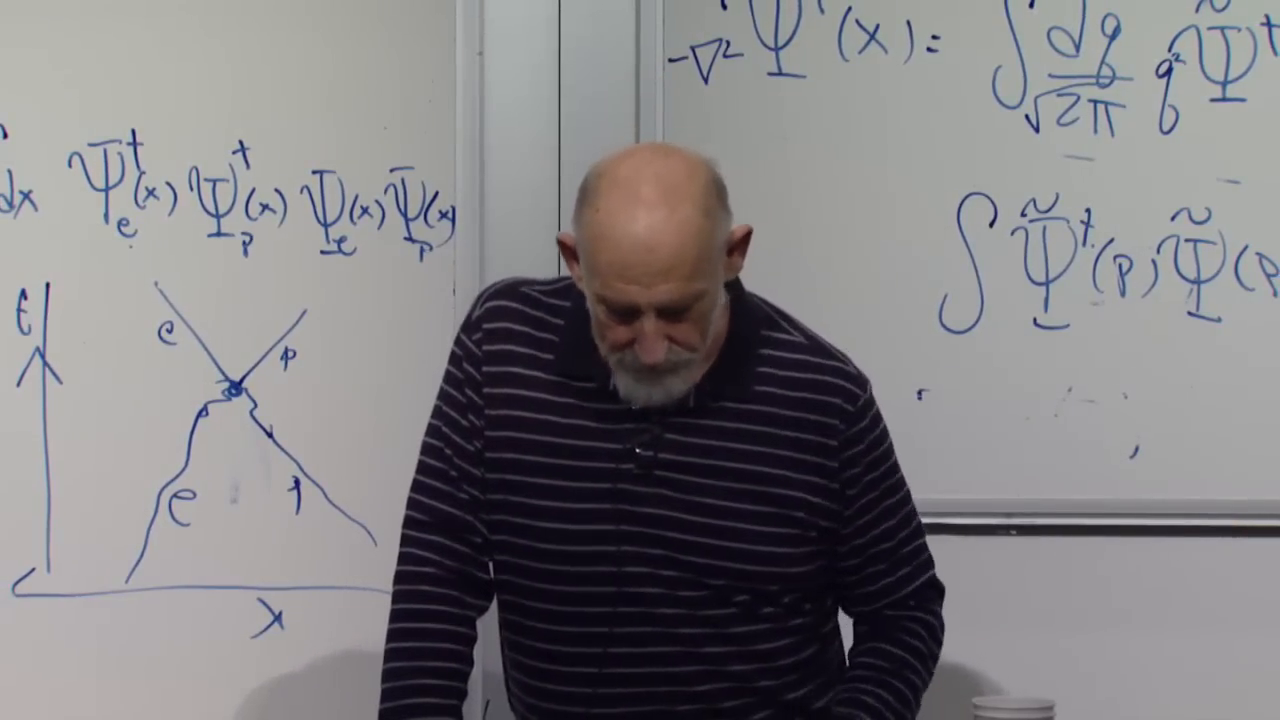
\includegraphics[width=0.94\linewidth]{lecture_09_frame_02.png}
\caption{تفاعل التماس على اللوح. تظهر المؤثرات الحقلية الموضعية الأربعة فوق مخطط الزمكان؛ ونقطة الالتقاء هي الموضع الوحيد الذي يؤثر فيه التفاعل المثالي.}
\lectureframe{00:35:36}
\end{figure}

\begin{figure}[htbp]
\centering
\begin{tikzpicture}[x=1.2cm,y=1.0cm,>=Latex]
\draw[->] (-3.0,0) -- (3.0,0) node[right] {$x$};
\draw[->] (0,-0.2) -- (0,4.2) node[above] {$t$};
\coordinate (v) at (0,2.0);
\fill (v) circle (1.8pt);
\draw[thick,->] (-2.2,0.4) -- (v);
\draw[thick,->] (2.0,0.4) -- (v);
\draw[thick,->] (v) -- (-1.6,3.7);
\draw[thick,->] (v) -- (2.2,3.7);
\node[left] at (-1.65,0.7) {$e$};
\node[right] at (1.55,0.7) {$p$};
\node[left] at (-1.15,3.3) {$e$};
\node[right] at (1.65,3.3) {$p$};
\node[right] at (0.12,2.05) {$g$};
\end{tikzpicture}
\caption{إعادة بناء واضحة لصورة التشتت الموضعي. والرأس اختزال للمؤثر في المعادلة~\eqref{eq:l9-contact}، وليس قانون تصادم كلاسيكيًا.}
\end{figure}

تتفاعل الإلكترونات والبروتونات الحقيقية عن بُعد عبر جهد كولوم. ونموذج التلامس ليس إلا الخطوة الأولى القصيرة: فإذا أظهرت التجربة أن نوعين من الجسيمات يتبعثران فقط عندما يتراكبان، فإن المعادلة~\eqref{eq:l9-contact} هي نوع الحد الذي سنضعه في الهاملتوني.

\begin{classroomqa}
\lecturetimestamp{00:35:40}
\audiencequestion{لماذا يكون مؤثر التبعثر هذا جزءًا من الهاملتوني إذا كانت الطاقة لا تتغير؟}
\lecturerresponse{الهاملتوني هو مؤثر الطاقة، وهو أيضًا المولِّد الذي يغيّر الحالة. فطاقة الوضع بين الجسيمين تُحدث التبعثر تحت التطور الزمني. ولا يعني انحفاظ الطاقة الكلية أن الحالة، أو زخوم الجسيمين كلٌّ على حدة، تبقى بلا تغير.}
\end{classroomqa}

وهذا يعطينا قاعدة عملية. تعلّم أولًا من التجربة ما العمليات الموضعية التي يمكن للجسيمات أن تخضع لها. ثم شفّر تلك العمليات في المؤثر الذي يحدّث الحالة. إن جداءات الحقول ليست جبرًا زخرفيًا: فالعوامل ذات الخناجر والعوامل من دون خناجر تحدد أي الأنواع تظهر وأيها تختفي.

\section{الاضمحلال، والعملية العكسية، والهيرميتية}

لنفترض أن حجرة فقاعات تكشف أثرًا للنوع \(A\) ينتهي عند نقطة تخرج منها آثار \(B\) و\(C\). العملية الموضعية هي
\begin{equation}
A\longrightarrow B+C.
\end{equation}
والمؤثر الذي ينفذها هو
\begin{equation}
V=g\int dx\,
\psi_B^\dagger(x)\psi_C^\dagger(x)\psi_A(x).
\label{eq:l9-decay-half}
\end{equation}
حقل الإفناء يزيل \(A\)؛ وحَقلا الإنشاء يُنتجان \(B\) و\(C\) عند النقطة نفسها. والتكامل بوزن متساوٍ على كل \(x\) يعبّر عن تناظر الانتقال المكاني ويعطي مباشرةً
\begin{equation}
p_A=p_B+p_C.
\end{equation}

يجب أن يكون الهاملتوني هيرميتيًا. وهذا ما يجعل \(e^{-itH}\) وحدويًا ويحفظ الاحتمال الكلي. والمعادلة~\eqref{eq:l9-decay-half} ليست هيرميتية بمفردها، لذلك يجب أن نضيف مرافقها:
\begin{equation}
H_{\mathrm{int}}
=\int dx\left[
g\,\psi_B^\dagger\psi_C^\dagger\psi_A
+g^*\,\psi_A^\dagger\psi_C\psi_B
\right](x).
\label{eq:l9-hermitian-vertex}
\end{equation}
إذا كان الاقتران \(g\) حقيقيًا، فالمعاملان متماثلان. وأخذ المرافق الهيرميتي يعكس ترتيب المؤثرات، فضلًا عن مبادلة الحقول ذات الخناجر بالحقول من دون خناجر. وفي هذا النموذج البوزوني المبسط، تتبادل حقول الأنواع المختلفة، لذلك لا يسبب هذا القلب أي تعقيد إضافي.

والحد الثاني ينفذ العملية العكسية،
\begin{equation}
B+C\longrightarrow A.
\end{equation}
وعليه، فإن هاملتونيًا مغلقًا ووحدويًا يتيح الاضمحلال يحتوي أيضًا على سعة إعادة الاتحاد. وهذا لا يعد بأن كلا الاتجاهين يحدثان لكل مجموعة مختارة من الزخوم الخارجية؛ فقد تجعل الطاقة وقوانين الانحفاظ الأخرى أحد الاتجاهين غير متاح حركيًا. وإنما يعني أن المؤثر ومرافقه كلاهما ينتميان إلى الديناميكيات.

\begin{classroomqa}
\lecturetimestamp{00:42:48}
\audiencequestion{هل يمكن أن يوجد استثناء للقاعدة التي تقضي بأن العملية العكسية مسموح بها أيضًا؟}
\lecturerresponse{ليس على مستوى هاملتوني هيرميتي لنظام مغلق: فالتآثر المرافق مطلوب. وقد يبقى تفاعل عكسي معين محجوبًا بالحركيات أو بعدد كمّي محفوظ آخر، لكن عنصر المصفوفة المرافق موجود.}
\end{classroomqa}

العدد \(g\) هو ثابت الاقتران. فإذا كان \(g\) صغيرًا، فإن الجسيمات التي تلتقي لا تتفاعل إلا تفاعلًا ضعيفًا؛ وإذا كان كبيرًا، كانت سعة الانتقال أكبر. وعادةً ما تكون الاقترانات معاملات تُقاس في التجارب، مع أن التناظرات قد تربط بين عدة اقترانات تبدو مختلفة ظاهريًا.

والنحو نفسه يعالج تفاعلات أشد تعقيدًا. ففي اضمحلال بيتا،
\begin{equation}
n\longrightarrow p+e^-+\bar\nu_e,
\end{equation}
يحتوي حد موضعي تخطيطي على أربعة حقول: أحدها يفني النيوترون، وثلاثة منها تنشئ البروتون والإلكترون وضديد نيوترينو الإلكترون، مع العملية المرافقة هيرميتيًا. وهذا يكفي لرؤية كيف تبدأ مجموعة صغيرة من أحاديات المؤثرات في تعريف نظرية حقل كمومي.

\section{لماذا يهم مربع الهاملتوني}

لقد احتفظت صيغة الزمن القصير \eqref{eq:l9-short-update} بالرتبة الأولى فقط في \(\epsilon\). والتوسع الكامل هو
\begin{equation}
e^{-i\epsilon H}
=1-i\epsilon H-\frac{\epsilon^2}{2}H^2
+\frac{i\epsilon^3}{3!}H^3+\cdots.
\label{eq:l9-exponential}
\end{equation}
وعند الرتبة الثانية يؤثر الهاملتوني مرتين. وهذا هو الأصل الجبري لأول صور العمليات المركبة.

بالنسبة للرأس \(A\leftrightarrow B+C\)، يمكن لفعل واحد أن يجمع \(B+C\) في \(A\)، ويمكن لفعل ثانٍ أن يفكك ذلك \(A\) من جديد إلى \(B+C\):
\begin{equation}
B+C\longrightarrow A\longrightarrow B+C.
\label{eq:l9-bc-scattering}
\end{equation}
والمساهمة الصافية هي سعة تبعثر \(B+C\to B+C\). أما \(A\) الوسيط فليس حدثًا مرصودًا إضافيًا؛ بل يوسم الحالة التي يُجمَع عليها بين فِعْلَي التفاعل.

\begin{classroomqa}
\lecturetimestamp{00:49:54}
\audiencequestion{هل ينبغي أن يحمل حقل \(C\) في الجداء المكتوب من الرتبة الثانية خنجرًا؟}
\lecturerresponse{نعم، يجب أن يطابق ترتيب المؤثرات التسلسل المذكور. فالرأس الأول يفني \(B\) و\(C\) وينشئ \(A\)؛ والثاني يفني \(A\) ويعيد إنشاء \(B\) و\(C\). إن كتابة الخناجر المناظرة على نحو صحيح تعيد هذا التفسير.}
\end{classroomqa}

\begin{figure}[htbp]
\centering
\includegraphics[width=0.94\linewidth]{lecture_09_frame_05.png}
\caption{الاتجاهان للرأس الابتدائي \(A\leftrightarrow B+C\) على اللوح. ووضعهما متجاورين هو الاختزال البصري للعملية من الرتبة الثانية في المعادلة~\eqref{eq:l9-bc-scattering}.}
\lectureframe{00:48:56}
\end{figure}

والآن أضف جسيم \(B\) متفرجًا. يتيح فعل واحد لـ\(A\) أن يصدر \(C\) ويتحول إلى \(B\)؛ ويتيح فعل لاحق لذلك \(C\) أن يتحد مع \(B\) الأصلي ليكوّن \(A\). والجسيمات الخارجية هي من جديد \(A+B\)، لكن زخومها يمكن أن تتغير. ونصف ذلك بأنه تبعثر \(A\) و\(B\) بتبادل \(C\).

\begin{figure}[htbp]
\centering
\includegraphics[width=0.94\linewidth]{lecture_09_frame_06.png}
\caption{بناء التبادل على اللوح. يَصل الرسم الموجود على اليمين بين رأسين ابتدائيين بخط داخلي لـ\(C\) بينما تتبعثر الجسيمات الخارجية \(A\) و\(B\).}
\lectureframe{00:51:22}
\end{figure}

\begin{figure}[htbp]
\centering
\begin{tikzpicture}[x=1.1cm,y=1cm,>=Latex]
\draw[->] (-3.7,-0.2) -- (-3.7,4.2) node[above] {$t$};
\coordinate (v1) at (-0.9,1.25);
\coordinate (v2) at (0.9,2.95);
\fill (v1) circle (1.7pt);
\fill (v2) circle (1.7pt);
\draw[thick,->] (-2.6,0.2) -- (v1) node[midway,below left] {$A$};
\draw[thick,->] (2.6,0.2) -- (v2) node[midway,below right] {$B$};
\draw[thick,->] (v1) -- (-2.4,4.0) node[midway,left] {$B$};
\draw[thick,->] (v2) -- (2.5,4.0) node[midway,right] {$A$};
\draw[thick,->,dashed] (v1) -- (v2) node[midway,above left] {$C$};
\node[below] at (0,-0.05) {$A+B\rightarrow A+B$};
\end{tikzpicture}
\caption{إعادة بناء واضحة لتبادل \(C\). تساهم كل نقطة بعامل واحد من \(g\)، ولذلك يكون هذا الحد من الرتبة الثانية متناسبًا مع \(g^2\).}
\end{figure}

تُسمى كل نقطة تفاعل موضعية رأسًا. ويسهم كل رأس بعامل من اقترانه، لذا تحمل مساهمة ذات رأسين \(g^2\)، وتحمل مساهمة ذات ثلاثة رؤوس \(g^3\)، وهكذا دواليك. ولذلك يربط حد واحد في الهاملتوني بين عائلة كبيرة من التفاعلات. وهذا الاقتصاد هو أحد أسباب قوة نظرية الحقل الكمومي إلى هذا الحد: فعدد صغير من التفاعلات الموضعية ينظم قدرًا هائلًا من بيانات التبعثر.

\begin{classroomqa}
\lecturetimestamp{00:53:14}
\audiencequestion{ماذا نسمي العملية \(A\to B+C\to A\)؟}
\lecturerresponse{إنها مساهمة في الطاقة الذاتية. فـ\(A\) المقاس ليس مجرد حالة الأساس العارية أحادية الجسيم؛ فالحالة المتفاعلة لها أيضًا سعة لمركبات قريبة من \(B+C\). وقد يكشف التبعثر منه تلك البنية الملبَّسة.}
\end{classroomqa}

تقدّم الديناميكا الكهربائية الكمية المثال المألوف. فرأس تآثر موضعي إلكترون--فوتون يمكنه أن يفني إلكترونًا، ويعيد إنشاء إلكترون، وينشئ فوتونًا. وعند الرتبة الثانية، قد يصدر الإلكترون فوتونًا ثم يعيد امتصاصه. ومن المغري أن نروي هذا على أنه فيلم صغير، لكن معناه المنضبط هو حد في التوسع الاضطرابي. والإلكترون الفيزيائي حالة ملبسة ذات مركبات تحتوي فوتونات.

إن التقدير الصفي بأن هذا المركب هو ``حوالي واحد في المئة'' ينقل المقياس الذي يحدده ثابت البنية الدقيقة، \(\alpha_{\mathrm{em}}\simeq 1/137\). ويعتمد احتمال دقيق لمركبة فوتونية في فضاء فوك على دقة الطاقة وعلى الكيفية التي تُعرَّف بها الحالة المتفاعلة؛ وليس خاصية كونية مقدارها واحد في المئة لإلكترون معزول. أما العبارة الراسخة فهي أن التفاعل يغير البنية القابلة للقياس للإلكترون.

\section{ما الذي يقوله المخطط وما الذي لا يقوله}

المخططات اختزال حسابي لقوى هاملتوني التفاعل. وليست تواريخ كلاسيكية موثوقة يؤدي فيها الجسيم حدثًا معينًا ثم آخر على نحو مؤكَّد. إن النظر إلى الداخل لتقرير أي بديل وسيط ``حدث حقًّا'' يغيّر التجربة ويدمر الجمع المتماسك، تمامًا كما في التداخل الكمومي المعتاد.

\begin{classroomqa}
\lecturetimestamp{00:56:52}
\audiencequestion{هل تُحفَظ الطاقة والزخم معًا عند الرأس الأول؟}
\lecturerresponse{في بناء الهاملتوني عند الزمن المتساوي المنفَّذ هنا، ينتج التكامل المكاني فورًا دالة دلتا للزخم. ولم يولد أي تكامل زمني بعدُ دالة دلتا للطاقة لذلك الإدراج المعزول. إن سعة التبعثر الكاملة الثابتة تحت الإزاحة الزمنية تحفظ الطاقة الكلية، في حين لا يلزم للخطوط الوسيطة أن تحقق علاقة على الغلاف الخاصة بالجسيمات المرصودة. وفي لغة المخططات التغايرية تُحفَظ رباعية الزخم عند كل رأس، لكن الجسيمات الداخلية قد تكون خارج الغلاف.}
\end{classroomqa}

إن الطاقة التي تبدو مفقودة في صورة ساذجة للرأس هي تحذير آخر من ألا نهمل طاقة التفاعل. فالهاملتوني الكلي أكثر من مجرد مجموع طاقات الجسيمات الحرة. وإذا نشأ التباس، فارجع إلى المعادلة~\eqref{eq:l9-exponential}: فالصورة تمثل حدًا في توسع التطور الزمني الوحدوي. وتوفر تقنية مخططات فاينمان الكاملة ترتيبًا زمنيًا منهجيًا، ومُنتشرات، وتكاملات، وعوامل تناظر، لكن الفيزياء الأساسية تبدأ هنا.

ويأخذ سؤال مطول المخطط على نحو حرفي أكثر مما ينبغي، إذ يقارن الفوتون المنبعث بالمجال الكهربائي المحيط بإلكترون يتحرك ببطء.

\begin{classroomqa}
\lecturetimestamp{00:58:26}
\audiencequestion{هل المجال الكهربائي للإلكترون على مسافة ما ناتج حرفيًا من فوتونات مشعّة؟ وكيف ينسجم ذلك مع التداخل وتأثير Aharonov--Bohm؟}
\lecturerresponse{الحقل الساكن أو الحقل الحثّي ليس سيلًا من فوتونات مشعّة حقيقية. تصف الكهروديناميكا الكمومية كلًا من الإشعاع وكساء الإلكترون الكهرومغناطيسي بالحقل نفسه، لكن الحالات الكمومية والحركيات المقابلة تختلف. بالنسبة إلى إلكترون فائق النسبية، يمكن لبعض مركبات الحقل أن تتصرف، على نحو مفيد، كدفق من فوتونات شبه حقيقية؛ أمّا بالنسبة إلى إلكترون بطيء، فإن نموذج مسار فوتون حرفي هو النموذج الخاطئ. كما أن تداخل الشقين وتأثير Aharonov--Bohm ظاهرتان حقليتان لا كلاسيكيتان أيضًا، لكنهما لا يحولان مخطط الطاقة الذاتية هذا إلى فيلم ميكانيكي.}
\end{classroomqa}

\begin{classroomqa}
\lecturetimestamp{01:01:28}
\audiencequestion{لماذا يفشل بالضبط نموذج كلاسيكي لهذا المخطط؟}
\lecturerresponse{لأن الحساب يجمع على نحو مترابط سعات جميع البدائل الوسيطة المسموح بها. تجعل الخبرة هذه الصور مألوفة حدسيًا، لكن محتواها الحرفي لا يتجاوز أبدًا التوسع المؤثري الذي يعرّفها. إنها طريقة مدمجة لحساب \(H^2,H^3,\ldots\)، وليست سجلًا لأحداث وسيطة مُشاهدة.}
\end{classroomqa}

\begin{classroomqa}
\lecturetimestamp{01:03:04}
\audiencequestion{هل يمكن أن ينشأ تآثر كولوم المعتاد بوصفه الحد الكلاسيكي لتبادل الفوتونات؟}
\lecturerresponse{نعم. إن تقييم السعة المناسبة المتوسطة بفوتون وأخذ النهاية الساكنة غير النسبية يعطيان كمون كولوم. والاشتقاق أكثر تقنية من هذا التخطيط المؤثري الحالي، ومع ذلك لا ينبغي أن يُقرأ على أنه فوتون يقفز حرفيًا بين جسيمين كلاسيكيين.}
\end{classroomqa}

\begin{classroomqa}
\lecturetimestamp{01:03:44}
\audiencequestion{هل تُحسب ثوابت الاقتران من جداءات الحقول؟}
\lecturerresponse{تكون قيمها العددية عادةً مُدخلات تجريبية. ويمكن للتناظر أن يقيّدها أو يربط بين اقترانات كانت ستبقى مستقلة لولا ذلك. وعندما تتنبأ مثل هذه العلاقة بالشدد النسبية لتفاعلات متميزة ويؤكدها التجريب، يكون هذا التوافق ذا دلالة خاصة.}
\end{classroomqa}

\begin{classroomqa}
\lecturetimestamp{01:04:48}
\audiencequestion{ما دور التناظر العرضي مقارنةً بالتناظر المعياري؟}
\lecturerresponse{يقيّد التناظر المعياري مباشرة البنية المسموح بها والعلاقات بين الاقترانات. أمّا التناظر العرضي فلا يُفرض على المستوى الأساسي، بل يظهر لأن جميع التفاعلات المسموح بها من الرتبة الأدنى تصادف أنها تحترمه. ومع ذلك يمكن أن تترتب عليه نتائج مهمة، مع أن أصله ومتانته يختلفان عن أصل التناظر المعياري ومتانته.}
\end{classroomqa}

هذا يكفي من نظرية الحقول غير النسبية في الوقت الحاضر. لقد وعدنا بالفرميونات. وبدلًا من أن نكممها تكميمًا ثانيًا مباشرة، سنفهم أولًا معادلة الجسيم الواحد النسبية التي يجب أن تحققها مؤثرات حقولها.

\section{لماذا يحتاج الإلكترون إلى النسبية}

ابدأ في بعد مكاني واحد. هذا ليس قيدًا واقعيًا، لكنه يزيل التعقيد الهندسي للسبين في ثلاثة أبعاد مع الحفاظ على الجبر الأساسي. كتلة الإلكترون صغيرة بما يكفي بحيث تصبح النسبية مهمة حتى في الذرات. ففي الهيدروجين تكون سرعته المميزة من رتبة
\begin{equation}
v\sim\alpha_{\mathrm{em}}c\approx 0.007c,
\end{equation}
أي قرابة واحد في المئة من سرعة الضوء. أمّا بالنسبة إلى الإلكترونات الداخلية في ذرة ثقيلة، فيصبح المقياس التقريبي \(v\sim Z\alpha_{\mathrm{em}}c\)، ولذلك قد تكون التصحيحات النسبية كبيرة. وسواء أكان الدافع الحاسم فضولًا تاريخيًا أم دقةً ذرية، فإن معادلة نسبية شبيهة بمعادلة Schr\"odinger ضرورية فيزيائيًا.

تبدأ الوصفة المعتادة للتكميم من العلاقة الكلاسيكية بين الطاقة والزخم. ففي الحالة غير النسبية،
\begin{equation}
E=\frac{p^2}{2m},
\end{equation}
وتؤدي الإحلالات
\begin{equation}
E\mapsto i\partial_t,
\qquad
p\mapsto-i\partial_x
\end{equation}
إلى
\begin{equation}
i\partial_t\varphi(x,t)
=-\frac{1}{2m}\partial_x^2\varphi(x,t).
\end{equation}

أمّا النسبية فتعطي، مع \(c=1\)،
\begin{equation}
E^2=p^2+m^2.
\label{eq:l9-rel-dispersion}
\end{equation}

\begin{figure}[htbp]
\centering
\includegraphics[width=0.94\linewidth]{lecture_09_frame_07.png}
\caption{الانتقال على اللوح من \(E=p^2/2m\) إلى العلاقة النسبية \(E^2=p^2+m^2\)، مع \(c=1\).}
\lectureframe{01:10:30}
\end{figure}

يؤدي تطبيق الإحلالات على العلاقة المربعة إلى
\begin{equation}
-\partial_t^2\varphi
=\left(-\partial_x^2+m^2\right)\varphi,
\label{eq:l9-klein-gordon}
\end{equation}
أو على نحو مكافئ
\begin{equation}
\left(\partial_t^2-\partial_x^2+m^2\right)\varphi=0.
\end{equation}
هذه هي معادلة Klein--Gordon. إنها معادلة حقل نسبية ذات معنى تام، ولا سيما لحقول السبين الصفري. لكن المعادلة المنشودة للإلكترون يجب أن تكون من الرتبة الأولى في الزمن،
\begin{equation}
i\partial_t\Psi=H\Psi,
\end{equation}
بحيث يولّد \(H\) نفسه، لا \(H^2\) فقط، التطور.

يمكن صوريًا أن نختار
\begin{equation}
H=\sqrt{-\partial_x^2+m^2}.
\end{equation}
يمكن تعريف الجذر التربيعي على نحو نظيف في فضاء الزخم، حيث يعمل بالضرب في \(\sqrt{p^2+m^2}\)، لكنه في فضاء الموضع مؤثر شبه تفاضلي لاموضعي. وهو ذو معنى تقني، لكنه غير مساعد من الناحية الجمالية للمعادلة الموضعية التي نبحث عنها. لذلك نبدأ من جديد.

\section{موجة عديمة الكتلة تسير إلى اليمين}

لنأخذ أولًا جسيمًا عديم الكتلة يتحرك إلى اليمين. تحقق طاقته الموجبة وزخمه
\begin{equation}
E=p
\qquad (c=1).
\end{equation}
ويعطي التكميم
\begin{equation}
i\partial_t\psi=-i\partial_x\psi,
\end{equation}
أو
\begin{equation}
(\partial_t+\partial_x)\psi=0.
\label{eq:l9-right-mover}
\end{equation}
وكل حل له الشكل
\begin{equation}
\psi(x,t)=f(x-t).
\end{equation}
ويبقى الشكل ثابتًا ويتحرك إلى اليمين بسرعة الضوء.

تظهر صعوبتان فورًا. أولًا، إذا سُمِح للمعادلة~\eqref{eq:l9-right-mover} أن تعمل على أنماط فورييه الاعتباطية، فللزخم السالب طاقة \(E=p<0\)، ولذلك لا يملك الهاملتوني حدًا أدنى. إن تقييدها يدويًا إلى \(p>0\) لا يُبقي إلا المتحركات إلى اليمين، وليس بعدُ نظرية الإلكترون التي نريدها. ثانيًا، المعادلة طريق في اتجاه واحد: فهي لا تحتوي على إلكترون عادي يتحرك إلى اليسار. سنعالج مشكلة اليمين واليسار أولًا ونترك الطاقات السالبة على حالها.

\section{مركبتان ومصفوفة ألفا}

أدخل سعتين،
\begin{equation}
\Psi(x,t)=
\begin{pmatrix}
\psi_1(x,t)\\[3pt]
\psi_2(x,t)
\end{pmatrix},
\end{equation}
حيث تكون \(\psi_1\) متحركة إلى اليمين وتكون \(\psi_2\) متحركة إلى اليسار في الحد العديم الكتلة:
\begin{align}
(\partial_t+\partial_x)\psi_1&=0,
&
(\partial_t-\partial_x)\psi_2&=0.
\end{align}
وتسمح ميكانيكا الكم أيضًا بتراكبات اعتباطية من الاثنتين. لذلك يمكن للجسيم أن يمتلك سعات لكلا الاتجاهين بدلًا من أن يحمل وسمًا كلاسيكيًا يُختار مرة واحدة وإلى الأبد.

تشبه درجة الحرية الإضافية الثنائية القيم السبين من حيث الجبر، لكنها في بعد واحد ليست عزمًا زاويًا عاديًا. عرّف
\begin{equation}
\alpha=
\begin{pmatrix}
1&0\\
0&-1
\end{pmatrix}
=\sigma_3.
\label{eq:l9-alpha}
\end{equation}
فالمتجه الذاتي الموافق لـ \(+1\) ينتقي المركبة المتحركة إلى اليمين، والمتجه الذاتي الموافق لـ \(-1\) ينتقي المركبة المتحركة إلى اليسار. وفي النظرية عديمة الكتلة يكون الهاملتوني ببساطة
\begin{equation}
H=\alpha p,
\end{equation}
وتجتمع المعادلتان في
\begin{equation}
i\partial_t\Psi=-i\alpha\partial_x\Psi.
\label{eq:l9-massless-dirac}
\end{equation}

\begin{classroomqa}
\lecturetimestamp{01:22:44}
\audiencequestion{ما اسم المصفوفة القطرية التي تميّز بين المركبتين؟}
\lecturerresponse{بوصفها مصفوفة باولي فهي \(\sigma_3\)، لا \(\sigma_1\). وفي ترميز ديراك لهذا البناء الحالي نسميها \(\alpha\). وجبرها هو جبر باولي المألوف، مع أن الوسم الفيزيائي هنا هو الاتجاه لا العزم الزاوي المغزلي.}
\end{classroomqa}

\begin{classroomqa}
\lecturetimestamp{01:23:32}
\audiencequestion{هل يكتسب هذا البناء معنىً هندسيًا أكثر في ثلاثة أبعاد، حيث يكون الاتجاه متجهًا؟}
\lecturerresponse{نعم. تتطلب المسألة ثلاثية الأبعاد مصفوفة لكل اتجاه مكاني، وتؤدي إلى بنية سبينورية أغنى. ومع ذلك فإن النموذج أحادي البعد دقيق تمامًا ضمن إطاره الخاص، ويعزل جبر اليمين واليسار الأساسي من دون ذلك التعقيد الإضافي.}
\end{classroomqa}

\begin{figure}[htbp]
\centering
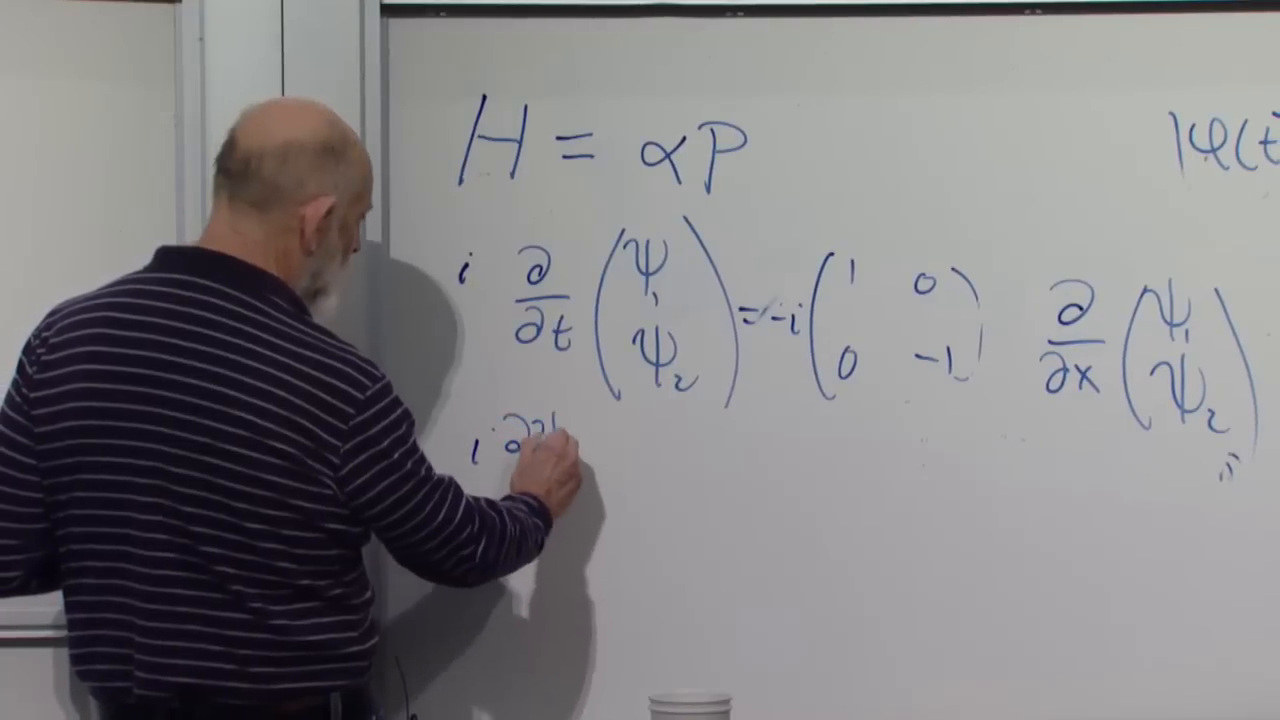
\includegraphics[width=0.94\linewidth]{lecture_09_frame_03.png}
\caption{معادلة المركبتين عديمة الكتلة على اللوح: \(H=\alpha P\)، حيث تسند المصفوفة القطرية انتشارًا متعاكسًا إلى \(\psi_1\) و\(\psi_2\).}
\lectureframe{01:26:00}
\end{figure}

زالت مشكلة الاتجاه الواحد. ويبقى طيف الطاقات السالبة، وقد اكتشفنا عيبًا ثالثًا: فما تزال المركبتان عديمتي الكتلة وتنتشران بسرعة الضوء. ولا بد في الخطوة التالية من إدخال طاقة سكون والاقتران بين الاتجاهين.

\section{إضافة الكتلة واكتشاف جبر ديراك}

أضف أبسط حد عام متناسب مع الكتلة،
\begin{equation}
H=\alpha p+\beta m,
\label{eq:l9-dirac-hamiltonian}
\end{equation}
حيث يعمل \(\beta\) فقط على المؤشر ذي المركبتين. وكان يمكن أن يكون مصفوفة الوحدة أو مصفوفة أخرى؛ ونَدَع علاقة التشتت النسبية تحسم ذلك.

بما أن \(H^2\) يجب أن يساوي \(p^2+m^2\)، فلنربع المعادلة~\eqref{eq:l9-dirac-hamiltonian}:
\begin{align}
H^2
&=(\alpha p+\beta m)^2\\
&=\alpha^2p^2+\beta^2m^2
+(\alpha\beta+\beta\alpha)pm.
\label{eq:l9-square-dirac}
\end{align}
تتبادل المصفوفات مع \(p\) لأنّها تؤثر في الحيز الداخلي ذي المركبتين، بينما يؤثر \(p\) في الدالة الموجية المكانية. ومطابقة المعادلة~\eqref{eq:l9-rel-dispersion} تستلزم
\begin{equation}
\alpha^2=\mathbb{1},
\qquad
\beta^2=\mathbb{1},
\qquad
\{\alpha,\beta\}
=\alpha\beta+\beta\alpha=0.
\label{eq:l9-dirac-algebra}
\end{equation}
الشرط الأول متحقق أصلًا من أجل \(\alpha=\sigma_3\). وأي مصفوفة باولي أخرى تحقق معها ضد التبادل، ومربعها يساوي مصفوفة الوحدة. اختر
\begin{equation}
\beta=
\begin{pmatrix}
0&1\\
1&0
\end{pmatrix}
=\sigma_1.
\label{eq:l9-beta}
\end{equation}
واختيار \(\sigma_1\) بدلًا من \(\sigma_2\) هو اصطلاح للأساس؛ فكلاهما يحقق الجبر نفسه بعد تغيير وحدوي للأساس.

\begin{classroomqa}
\lecturetimestamp{01:33:00}
\audiencequestion{هل أدرك ديراك ببساطة أن مصفوفات باولي تحقق هذه الشروط الجبرية؟}
\lecturerresponse{أُجري الاشتقاق التاريخي مباشرة في ثلاثة أبعاد، وأُدخلت فيه مصفوفات تحقق العلاقات المطلوبة. وبمجرد أن تُكتب الشروط، يجعل جبر باولي الحل في بعد واحد فوريًا: اختر مصفوفتين مختلفتين من مصفوفات باولي.}
\end{classroomqa}

\begin{classroomqa}
\lecturetimestamp{01:34:24}
\audiencequestion{هل هذا \(\beta\) هو معامل السرعة النسبي \(v/c\)؟}
\lecturerresponse{لا. بل هو مصفوفة تؤثر في مكوّنات السبينور. والحرف المعاد استخدامه ليس إلا ترميز ديراك؛ ولا علاقة له بالكمية الحركية \(v/c\).}
\end{classroomqa}

في ثلاثة أبعاد مكانية، لا تكفي مصفوفات \(2\times2\) للمجموعة الكاملة المطلوبة من المصفوفات المتضادة التبادل. ويُؤجَّل هذا التوسيع. وفي بُعد واحد، تكفي المعادلتان ~\eqref{eq:l9-alpha} و\eqref{eq:l9-beta}.

\section{معادلة ديراك المقترنة في بُعد واحد}

وبالتعويض بـ\(p=-i\partial_x\) نحصل على معادلة ديراك في بُعد واحد بصيغة هاملتونية:
\begin{equation}
i\partial_t\Psi
=\left(-i\alpha\partial_x+\beta m\right)\Psi.
\label{eq:l9-one-dimensional-dirac}
\end{equation}
ولأن \(\alpha\) قطرية، فإن حدَّ المشتقة المرتبط بها يُبقي المركبتين منفصلتين. ولأن \(\beta\) خارج القطر، فإن حدَّ الكتلة يبدّل إحداهما بالأخرى. وعند كتابتها مركبةً فمركبةً،
\begin{align}
i\partial_t\psi_1
&=-i\partial_x\psi_1+m\psi_2,
\label{eq:l9-dirac-component-one}\\
i\partial_t\psi_2
&=+i\partial_x\psi_2+m\psi_1.
\label{eq:l9-dirac-component-two}
\end{align}

\begin{figure}[htbp]
\centering
\includegraphics[width=0.94\linewidth]{lecture_09_frame_08.png}
\caption{معادلتا المركبتين المقترنتان على اللوح. تُرمِّز إشارتا المشتقة المتعاكستان إلى الحركة نحو اليمين ونحو اليسار؛ وحدُّ الكتلة خارج القطر يبدّل بين \(\psi_1\) و\(\psi_2\).}
\lectureframe{01:37:44}
\end{figure}

لا تعود المركبتان تتطوران على نحو مستقل ما إن \(m\ne0\). ومن تربيع المعادلة من الرتبة الأولى نستعيد مؤثر كلاين--غوردون على كل مركبة،
\begin{equation}
\left(\partial_t^2-\partial_x^2+m^2\right)\psi_a=0,
\qquad a=1,2,
\end{equation}
وتحقق الموجات المستوية \(E^2=p^2+m^2\). وتكون سرعتها الزمرية
\begin{equation}
v_g=\frac{dE}{dp}=\frac{p}{E},
\end{equation}
ويكون مقدارها أقل من الواحد عند كتلة غير منعدمة.

العلاقة بين الكتلة والخلط بين اليسار واليمين ليست مصادفة. فالمتحرك العديم الكتلة إلى اليمين يبقى متحركًا إلى اليمين تحت كل تعزيز لورنتزي صحيح؛ ولا يستطيع أي راصد دون ضوئي أن يسبق الضوء ويعكس اتجاهه. أما الجسيم ذو الكتلة فيمكن الإتيان به إلى السكون ثم النظر إليه من إطار أسرع يتحرك في الاتجاه نفسه، حيث تبدو سرعته معكوسة. ولذلك لا يمكن لنظرية نسبية ذات كتلة أن تُبقي قطاعي اليمين واليسار معزولين على الدوام. وحدُّ الكتلة خارج القطر يوفّر بالضبط الاقتران المطلوب.

\begin{classroomqa}
\lecturetimestamp{01:40:01}
\audiencequestion{هل يُعدّ تبديل المركبتين تذبذبًا كيراليًا؟}
\lecturerresponse{في هذا الأساس أحادي البعد، يميّز \(\alpha\) بين الاتجاهين الكيراليين في الحالة عديمة الكتلة. وحدُّ الكتلة خارج القطر يمزجهما، لذا لم تعد الكيرالية محفوظة. وبهذا المعنى فإن حدَّ الكتلة هو مصدر التذبذب الكيرالي.}
\end{classroomqa}

\begin{classroomqa}
\lecturetimestamp{01:40:46}
\audiencequestion{لماذا ينبغي أن تكون معادلة فرميون الجذر التربيعي لمعادلة بوزونية؟}
\lecturerresponse{لا ينبغي فهم الأمر على هذا النحو. فعلاقة التشتت \(E^2=p^2+m^2\) تنطبق على كل جسيم حر نسبي، بصرف النظر عن الإحصاء. ويصادف أن مؤثر ديراك يوفّر تحليلاً مصفوفيًا لمؤثر كلاين--غوردون، لكن تلك العلاقة الجبرية لا تشتق الفرميونات من البوزونات.}
\end{classroomqa}

\begin{classroomqa}
\lecturetimestamp{01:41:31}
\audiencequestion{هل يمكن اختزال المعادلة إلى تحليل قياسي بسيط إلى عاملين منفصلين، أحدهما للحركة نحو اليسار والآخر للحركة نحو اليمين؟}
\lecturerresponse{فقط في حد انعدام الكتلة تنفصل المعادلتان الكيراليتان إلى عاملين قياسيين مستقلين. أما عندما \(m\ne0\)، فإن التحليل المفيد يكون مصفوفيًا: فمصفوفتا \(\alpha\) و\(\beta\) المتضادتان في التبادل هما اللتان تزيلان الحد المتقاطع غير المرغوب فيه.}
\end{classroomqa}

\begin{classroomqa}
\lecturetimestamp{01:42:04}
\audiencequestion{هل تشكل هاتان المعادلتان المقترنتان بالفعل معادلة ديراك؟}
\lecturerresponse{نعم. فهما معًا تمثلان معادلة ديراك في بُعد مكاني واحد، ويمكن كتابتهما بصورة مكافئة في الصيغة الموجزة للمعادلة ~\eqref{eq:l9-one-dimensional-dirac}. ويمكن الحصول على تدوين تغايري أكثر تناظرًا بالضرب في \(\beta\)، لكن يُؤجَّل تقديم ذلك الشكل.}
\end{classroomqa}

تبقى مهمتان غير منجزتين عمدًا. فهذا البناء لم يزل الطاقات السالبة؛ بل أعطى حلولًا سالبة الطاقة في كلا القطاعين الاتجاهيين، ولذلك أصبحت تلك المشكلة الآن أشد بروزًا لا أقل. وما تزال النظرية تعيش في بُعد مكاني واحد. والخطوتان التاليتان هما تفسير حلول الطاقة السالبة وتوسيع جبر المصفوفات إلى أبعاد \(3+1\).

\chapter{الفرميونات، ومصفوفات ديراك، وبحر ديراك}

بحر ديراك هو وجهتنا، لكن الطريق إليه مهم. قبل مواجهة الطاقة السالبة في النظرية النسبية للإلكترون، نحتاج إلى أداتين. أولًا يأتي جبر المؤثرات الذي يميز الفرميونات عن البوزونات. ثم تأتي مراجعة لمعادلة ديراك أحادية البعد، حيث يمكن رؤية كل توسيع للدالة الموجية من غير هندسة الأبعاد المكانية الثلاثة. وما إن يكتمل هذان العنصران حتى تفرض المعادلة ثلاثية الأبعاد بنيتها المصفوفية الخاصة، ويعود النقاش الافتتاحي عن حالات الفرميونات المملوءة والفارغة بوصفه المفتاح إلى البوزيترونات.

نستخدم \(c=\hbar=1\). ويدل الرمز الكبير \(P\) على مؤثر الزخم، ويدل الرمز الصغير \(p\) على قيمة ذاتية للزخم، وتدل الرموز الغليظة على نظائرهما ثلاثية الأبعاد.

\section{يتحول التبادل إلى جبر المؤثرات}

لننظر في جسيمين متماثلين، أحدهما عند \(x\) والآخر عند \(y\). ويدل الرمزان \(x\) و\(y\) على موضعين كاملين؛ وليسا إحداثيين ديكارتيين لجسيم واحد. وعند التأثير بمؤثري إنشاء على حالة الفراغ نحصل على
\begin{equation}
\lvert x,y\rangle
=
\psi^\dagger(x)\psi^\dagger(y)\lvert0\rangle.
\label{eq:l10-two-particle-state}
\end{equation}

في حالة البوزونات، يترك تبديل الخانتين الحالة من دون تغير:
\begin{equation}
\lvert x,y\rangle=\lvert y,x\rangle.
\end{equation}
وعلاقة المؤثرات التي تضمن هذا التناظر هي
\begin{equation}
\psi^\dagger(x)\psi^\dagger(y)
=
\psi^\dagger(y)\psi^\dagger(x).
\label{eq:l10-boson-exchange}
\end{equation}
مؤثرا الإنشاء البوزونيان متبادلان، لذا يمكننا عكس ترتيبهما من دون تغيير الحالة التي ينشئانها.

في حالة الفرميونات، يغير التبادل الإشارة:
\begin{equation}
\lvert x,y\rangle=-\lvert y,x\rangle.
\label{eq:l10-fermion-state-exchange}
\end{equation}
الإشارة الكلية لمتجه حالة معزول غير قابلة للرصد، لكن الإشارات النسبية بين البدائل قابلة للرصد، لذا يجب الاحتفاظ بإشارة السالب هذه باتساق. وتقتضي المعادلة~\eqref{eq:l10-fermion-state-exchange}
\begin{equation}
\psi^\dagger(x)\psi^\dagger(y)
=
-\,\psi^\dagger(y)\psi^\dagger(x).
\label{eq:l10-fermion-operator-exchange}
\end{equation}

\begin{figure}[htbp]
\centering
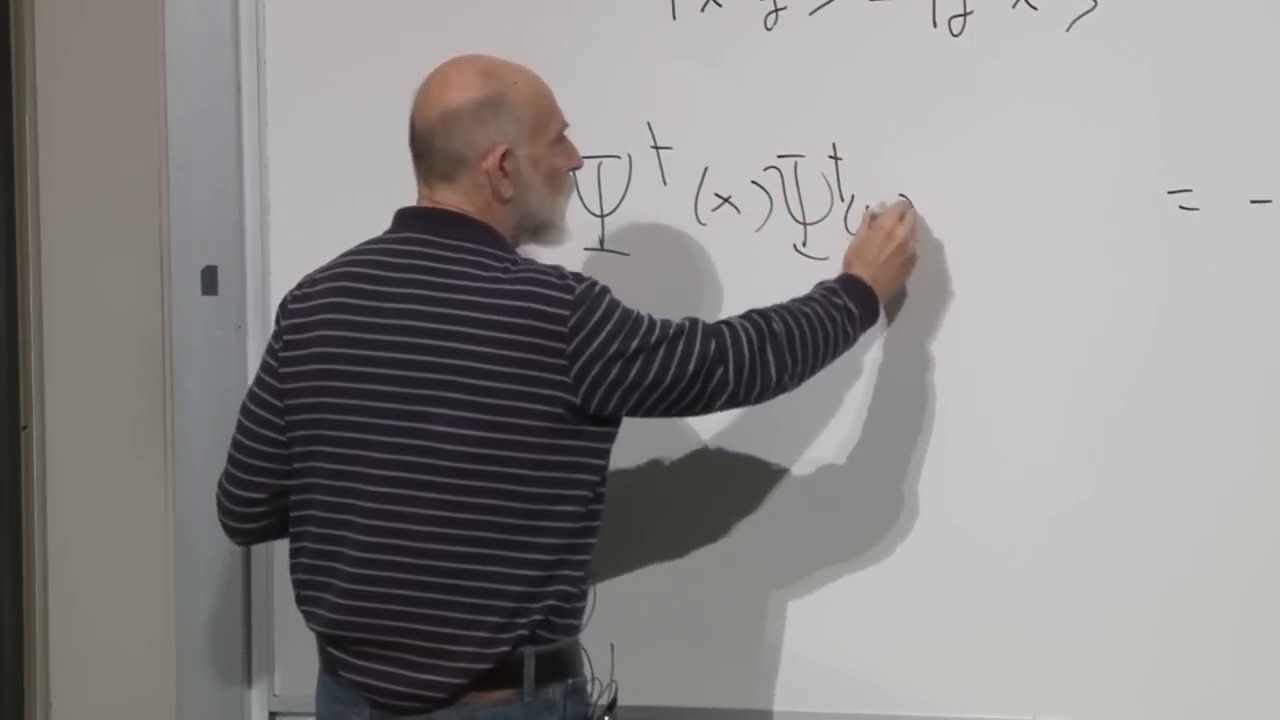
\includegraphics[width=0.94\linewidth]{lecture_10_figure_02.png}
\caption{العلاقة المكتوبة على اللوح التي تحقق التبادل الفرميوني. إن تبديل مؤثري الإنشاء يعكس إشارة حالة الجسيمين.}
\lectureframe{00:05:50}
\end{figure}

بالنسبة إلى أي مؤثرين \(A\) و\(B\)، نعرّف المبدلة المضادة بـ
\begin{equation}
\{A,B\}:=AB+BA.
\end{equation}
ولذلك تكون قاعدة التبادل
\begin{equation}
\{\psi^\dagger(x),\psi^\dagger(y)\}=0.
\label{eq:l10-creation-anticommutator}
\end{equation}
ويستبدل جبر الحقل الفرميوني المناظر المبدلات البوزونية بالمبدلات المضادة. ويجب التمييز بين استعمالين لهذه الكلمة: فمؤثرات الحقل تتبادل تبادلًا مضادًا بسبب إحصاء فيرمي، أما المصفوفات فستفعل ذلك لاحقًا من أجل إلغاء الحدود المتقاطعة في علاقة تشتت نسبية.

والآن ضع \(y=x\) في المعادلة~\eqref{eq:l10-creation-anticommutator}. ويصبح الضربان متماثلين:
\begin{align}
0
&=\{\psi^\dagger(x),\psi^\dagger(x)\}\\
&=2\,\psi^\dagger(x)\psi^\dagger(x).
\end{align}
ومن ثم
\begin{equation}
\bigl(\psi^\dagger(x)\bigr)^2=0.
\label{eq:l10-exclusion}
\end{equation}
إن محاولة إنشاء فرميونين متماثلين في حالة الجسيم الواحد نفسها تعطي متجه الصفر. وهذا هو مبدأ الاستبعاد في صيغة مؤثرية.

\begin{figure}[htbp]
\centering
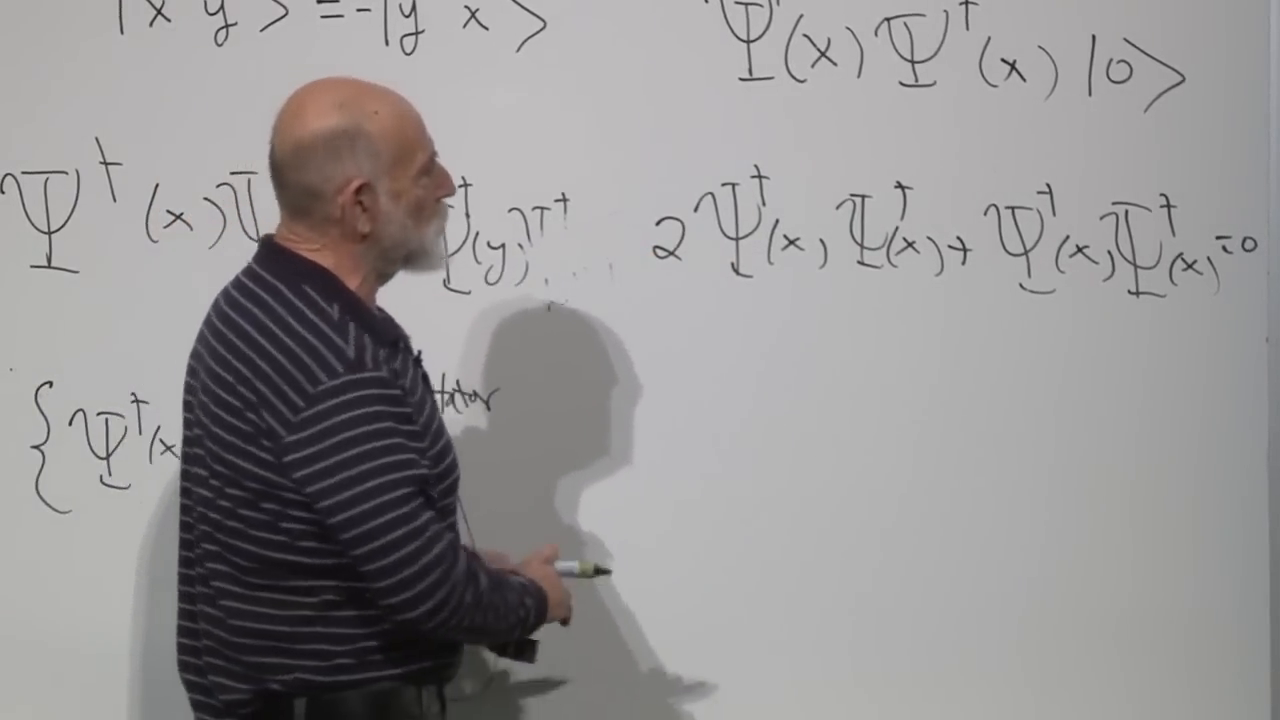
\includegraphics[width=0.94\linewidth]{lecture_10_figure_03.png}
\caption{التخصيص عند تساوي الحالتين على اللوح. يظهر حاصل ضرب مؤثر الخلق المكرَّر مرتين، ولذلك لا بد أن يساوي الصفر.}
\lectureframe{00:08:04}
\end{figure}

\begin{figure}[htbp]
\centering
\begin{adjustbox}{max width=\linewidth}
\begin{tikzpicture}[node distance=1.25cm,>=Latex]
\node[draw,rounded corners,align=center,inner sep=7pt] (a)
  {$\{\psi^\dagger(x),\psi^\dagger(x)\}=0$};
\node[draw,rounded corners,align=center,inner sep=7pt,right=of a] (b)
  {$2(\psi^\dagger(x))^2=0$};
\node[draw,rounded corners,align=center,inner sep=7pt,right=of b] (c)
  {$(\psi^\dagger(x))^2=0$};
\draw[->,thick] (a) -- (b);
\draw[->,thick] (b) -- (c);
\end{tikzpicture}
\end{adjustbox}
\caption{إعادة بناء حجة الاستبعاد من دون خطوات اللوح الوسيطة التي مُحيت جزئيًا.}
\end{figure}

\section{لماذا تكون حالتا الامتلاء والفراغ متناظرتين لفرميون}

ثمّة فرق ثانٍ بين المؤثرات البوزونية والفرميونية، وهو أدق من مبدأ الاستبعاد وجوهري لاحقًا. لنمط بوزوني واحد،
\begin{equation}
[a,a^\dagger]=1,
\qquad
n=0,1,2,\ldots.
\end{equation}
فإن تبديل \(a\) و\(a^\dagger\) يغيّر إشارة المبادل. وحتى لو لم يُسمَّ المؤثران إلا \(A\) و\(B\)، لأخبرتنا الجبرية أيُّ ترتيب يرفع عدد الإشغال وأيُّه يخفضه.

ولسُلَّم الإشغال البوزوني اتجاه أيضًا. فمؤثر الإبادة يبلغ في النهاية \(\lvert0\rangle\) ويعطي صفرًا، في حين يمكن لمؤثر الخلق أن يستمر إلى ما لا نهاية:
\begin{align}
a\lvert0\rangle&=0,\\
a^\dagger\lvert n\rangle&\propto\lvert n+1\rangle,
\qquad n=0,1,2,\ldots.
\end{align}
وقلب هذا السلم رأسًا على عقب لا يعيد إنتاج الطيف نفسه. فله قاع ولا قمة له.

ولنمط فرميوني واحد،
\begin{equation}
\{a,a^\dagger\}=1,
\qquad
a^2=(a^\dagger)^2=0,
\qquad
n=0,1.
\label{eq:l10-fermion-mode}
\end{equation}
ينقل مؤثر الخلق الحالة الفارغة إلى الحالة الممتلئة ثم يتوقف:
\begin{equation}
a^\dagger\lvert0\rangle=\lvert1\rangle,
\qquad
a^\dagger\lvert1\rangle=0.
\end{equation}
ويقوم مؤثر الإبادة بالعكس:
\begin{equation}
a\lvert1\rangle=\lvert0\rangle,
\qquad
a\lvert0\rangle=0.
\end{equation}
لا توجد إلا حالتان، لذا يكون المخطط متناظرًا تحت تبديل الحالة الممتلئة بالحالة الفارغة و\(a\) بـ\(a^\dagger\). وما يزال للمؤثرين معنيان فيزيائيان مختلفان، لكن جبريتهما لم تعد تميّز أحدهما بوصفه مؤثر خلق والآخر بوصفه مؤثر إبادة. وهذا التناظر الصوري هو بذرة إعادة تأويل الجسيم-الفجوة.

\begin{classroomqa}
\lecturetimestamp{00:13:54}
\audiencequestion{إذا كان \((a^\dagger)^2=0\)، أفهذا تناقض، أم إنه يستلزم أن \(a^\dagger=0\)؟}
\lecturerresponse{لا هذا ولا ذاك. يمكن لمؤثر غير صفري أن يكون له مربع منعدم. هنا يأخذ \(a^\dagger\) \(\lvert0\rangle\) إلى \(\lvert1\rangle\)، ولكن لا توجد حالة مسموح بها فوق \(\lvert1\rangle\)، لذلك فإن تطبيقه مرتين يعطي صفرًا. والاستدلال نفسه يعطينا \(a^2=0\).}
\end{classroomqa}

احتفظ بهذا التناظر بين الحالتين الممتلئة والفارغة جانبًا. فعندما يُزال إلكترون سالب الطاقة، ستُعاد تسمية مؤثر الإبادة بوصفه مؤثر خلق بوزيترون. وليست هذه الخطوة تغييرًا اعتباطيًا في الترميز؛ بل إنها تستخدم على وجه الدقة جبر الفرميون ذي الحالتين الذي أُرسي هنا.

\section{بناء ديراك أحادي البعد}

لنعد الآن إلى جسيم واحد في بعد مكاني واحد. أبسط معادلة موجية نسبية من الرتبة الأولى هي
\begin{equation}
i\partial_t\psi=-\,i\partial_x\psi.
\label{eq:l10-right-mover}
\end{equation}
ومع \(P=-i\partial_x\) تصبح
\begin{equation}
H=P.
\end{equation}
ولحالة ذاتية للزخم يكون \(E=p\)، وتكون سرعتها الزمرية
\begin{equation}
v_g=\frac{dE}{dp}=1.
\end{equation}
فالزخم الموجب أو السالب، ومن ثم الطاقة الموجبة أو السالبة، ما يزال يعطي موجة تتحرك كوحدة واحدة إلى اليمين. إشارة \(p\) تغيّر نمط الطور، لا اتجاه الانتشار.

يجب أن يكون الجسيم ذو الكتلة قادرًا على الحركة في أيٍّ من الاتجاهين. أدخل مركبةً ثانية تحقق
\begin{equation}
H\psi_1=P\psi_1,
\qquad
H\psi_2=-P\psi_2.
\label{eq:l10-two-directions}
\end{equation}
تتحرك المركبة الأولى إلى اليمين، والثانية إلى اليسار. ضعْهما في عمود،
\begin{equation}
\Psi=
\begin{pmatrix}
\psi_1\\
\psi_2
\end{pmatrix},
\end{equation}
وعرّف
\begin{equation}
\alpha=
\begin{pmatrix}
1&0\\
0&-1
\end{pmatrix}.
\end{equation}
فتصبح المعادلتان
\begin{equation}
H\Psi=\alpha P\Psi.
\label{eq:l10-massless-one-d}
\end{equation}
وثمن إدراج الاتجاهين معًا هو درجة حرية داخلية جديدة ثنائية القيمة.

الاتجاه وحده لا يولِّد كتلة. أدخل مصفوفةً ثانية،
\begin{equation}
\beta=
\begin{pmatrix}
0&1\\
1&0
\end{pmatrix},
\end{equation}
وجرِّب
\begin{equation}
H=\alpha P+\beta m.
\label{eq:l10-massive-one-d}
\end{equation}
وتحقق المصفوفتان
\begin{equation}
\alpha^2=\beta^2=\mathbb{1},
\qquad
\{\alpha,\beta\}=0.
\label{eq:l10-one-d-algebra}
\end{equation}
ويعطي تربيع الهاملتوني
\begin{align}
H^2
&=(\alpha P+\beta m)^2\\
&=\alpha^2P^2+\beta^2m^2
  +(\alpha\beta+\beta\alpha)Pm\\
&=P^2+m^2.
\label{eq:l10-one-d-dispersion}
\end{align}
ويزيل المُبدِّل المضاد في المعادلة ~\eqref{eq:l10-one-d-algebra} الحدَّ غير المرغوب فيه الخطي في كلٍّ من \(P\) و\(m\).

المصفوفة غير القطرية \(\beta\) تقرن المركبتين الاتجاهيتين. ومن المفيد أن نتصور حد الكتلة على أنه يمزج باستمرار بين السعات المتحركة إلى اليمين والمتحركة إلى اليسار. ولا ينبغي أخذ هذه الصورة على نحو حرفي بوصفها جسيمًا يرتد ذهابًا وإيابًا على مسار مجهري، لكنها تبيّن لماذا يمكن لحزمة موجية ذات كتلة أن يكون لها متوسط سرعة دون سرعة الضوء وأن تمتلك إطار سكون، في حين أن مركبة كيرالية معزولة عديمة الكتلة لا تستطيع ذلك.

\begin{classroomqa}
\lecturetimestamp{00:23:37}
\audiencequestion{هل توجد دلالة فيزيائية أعمق لإدخال كلتا المركبتين الاتجاهيتين؟}
\lecturerresponse{نعم، ولكنها تظهر بوضوح أكبر في ثلاثة أبعاد. في هذه المرحلة هما مجرد المركبتين اللازمتين لوصف الانتشار في اتجاهين متعاكسين وللسماح باقتران كتلي غير قطري. وتفسيرهما اللاحق هو اليدوية، أو الكيرالية.}
\end{classroomqa}

\section{تفرض الأبعاد الثلاثة مصفوفات باولي}

في ثلاثة أبعاد مكانية، يكون الزخم متجهًا. ولذلك فإن هاملتونيًا خطيًا في الزخم وقياسيًا تحت الدورانات يوحي بمتجه آخر، هذه المرة متجهًا مركباته مصفوفات:
\begin{equation}
H=\boldsymbol{\alpha}\cdot\mathbf P
=\alpha_xP_x+\alpha_yP_y+\alpha_zP_z.
\label{eq:l10-three-d-ansatz}
\end{equation}

\begin{figure}[htbp]
\centering
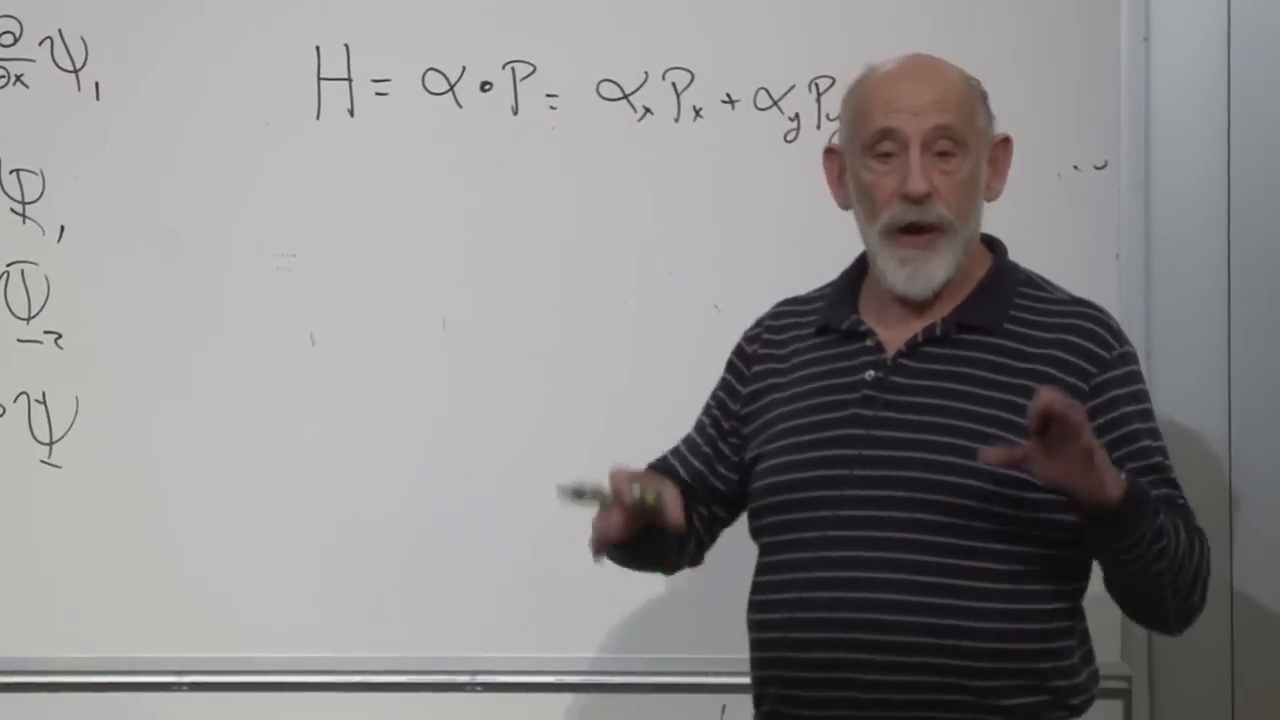
\includegraphics[width=0.94\linewidth]{lecture_10_figure_04.png}
\caption{الافتراض الابتدائي الثلاثي الأبعاد عديم الكتلة \(H=\boldsymbol{\alpha}\cdot\mathbf P\) عند النقطة التي تصبح فيها مصفوفة واحدة متجهًا مؤلفًا من ثلاث مصفوفات.}
\lectureframe{00:26:00}
\end{figure}

لنبدأ من جديد بالحالة عديمة الكتلة. نحتاج إلى
\begin{equation}
H^2=\mathbf P^2=P_x^2+P_y^2+P_z^2.
\end{equation}
وبتوسيع مربع المعادلة ~\eqref{eq:l10-three-d-ansatz}،
\begin{align}
H^2
&=\alpha_x^2P_x^2+\alpha_y^2P_y^2\\
&\quad+\alpha_z^2P_z^2\\
&\quad+\{\alpha_x,\alpha_y\}P_xP_y\\
&\quad+\{\alpha_x,\alpha_z\}P_xP_z\\
&\quad+\{\alpha_y,\alpha_z\}P_yP_z.
\end{align}
تكون الحدود القطرية صحيحة إذا تحقق
\begin{equation}
\alpha_x^2=\alpha_y^2=\alpha_z^2=\mathbb{1},
\end{equation}
وتختفي جميع الحدود المتصالبة إذا تحقق
\begin{equation}
\{\alpha_i,\alpha_j\}=0,
\qquad i\ne j.
\label{eq:l10-alpha-anticommutation}
\end{equation}

ثلاث مصفوفات مألوفة \(2\times2\) تحقق ذلك تمامًا:
\begin{equation}
\sigma_x=
\begin{pmatrix}
0&1\\
1&0
\end{pmatrix},
\quad
\sigma_y=
\begin{pmatrix}
0&-i\\
i&0
\end{pmatrix},
\quad
\sigma_z=
\begin{pmatrix}
1&0\\
0&-1
\end{pmatrix}.
\label{eq:l10-pauli-matrices}
\end{equation}
وعليه فإن أحد الحلول هو
\begin{equation}
\alpha_i=\sigma_i,
\qquad
H=\boldsymbol{\sigma}\cdot\mathbf P.
\label{eq:l10-weyl-hamiltonian}
\end{equation}

\begin{figure}[htbp]
\centering
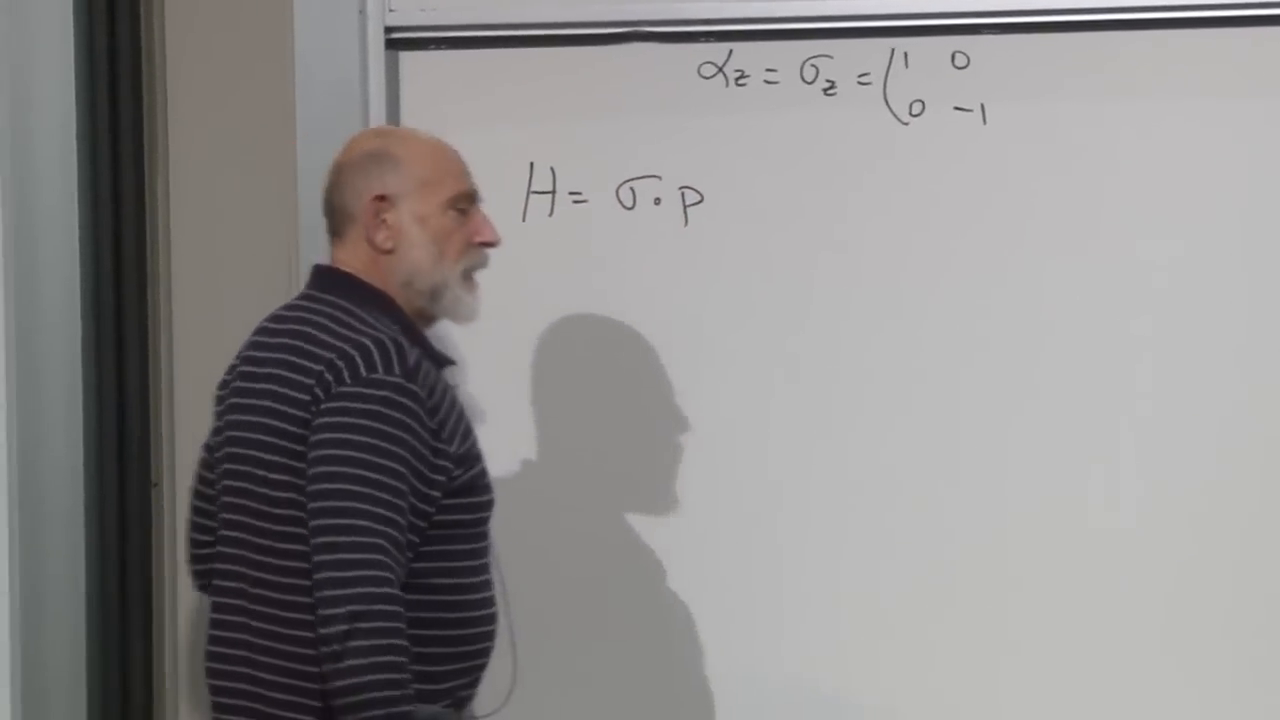
\includegraphics[width=0.94\linewidth]{lecture_10_figure_05.png}
\caption{الهاملتوني المدمج عديم الكتلة \(H=\boldsymbol{\sigma}\cdot\mathbf P\)، مع بقاء \(\alpha_z=\sigma_z\) ظاهرًا فوقه.}
\lectureframe{00:28:16}
\end{figure}

لحالة ذاتية للزخم،
\begin{equation}
\boldsymbol{\sigma}\cdot\mathbf p
=
|\mathbf p|\,\boldsymbol{\sigma}\cdot\widehat{\mathbf p}.
\end{equation}
للمؤثر \(\boldsymbol{\sigma}\cdot\widehat{\mathbf p}\) القيم الذاتية \(+1\) و\(-1\)، ولذلك
\begin{equation}
E=\pm|\mathbf p|.
\end{equation}
في هذه النظرية ذات المركبتين، تكون درجة الحرية الباولية في حالة الطاقة الموجبة مصطفةً مع الزخم، بينما تكون في حالة الطاقة السالبة مصطفةً بعكس اتجاهه. وهذا الاصطفاف مقيد؛ وليس اتجاهاً للّف المغزلي يمكن ضبطه على نحو مستقل عند تثبيت إشارة الطاقة.

\begin{classroomqa}
\lecturetimestamp{00:30:10}
\audiencequestion{هل ينبثق اللف المغزلي من معادلة ديراك، أم أُدخل فيها لأن من المعروف سلفاً أن للإلكترون عزماً مغناطيسياً؟}
\lecturerresponse{هنا تعني عبارة «ينبثق» «ينشأ كنتيجة»، لا «يختفي». كان الشرط الابتدائي أن يكون لدينا هاملتوني خطي في الزخم يكون مربعه \(\mathbf P^2\). ولا تستطيع الأعداد العادية أن تحقق الجبر المطلوب، لكن مصفوفات باولي تستطيع ذلك. ومن ثم فإن بنيتها ذات المركبتين تظهر مع عملية جعله خطيًا نفسها. وهذا لا يثبت أن كل جسيم يجب أن يملك لفًا مغزليًا؛ بل يقول إن الجسيمات التي تصفها هذه المعادلة من نوع ديراك تحمل درجة الحرية السبينورية المناظرة.}
\end{classroomqa}

هذه إحدى الدروس المركزية في هذا البناء. ليست المصفوفات تسميات زخرفية تُضاف بعد العثور على المعادلة النسبية. بل إن محاولة أخذ جذر تربيعي موضعي لعلاقة التشتت النسبية هي التي تولّدها.

\section{لماذا تتطلب الكتلة أربعة مركبات}

جرّب أن تكرر بناء الكتلة أحادي البعد من دون توسيع نظرية \(2\times2\):
\begin{equation}
H=\boldsymbol{\sigma}\cdot\mathbf P+\beta m.
\label{eq:l10-failed-mass}
\end{equation}
افترض \(\beta^2=\mathbb{1}\). يحتوي مربعه على الحدود المطلوبة \(\mathbf P^2+m^2\)، لكنه يحتوي أيضًا على
\begin{equation}
m\sum_i\{\sigma_i,\beta\}P_i.
\end{equation}
ولإزالة هذا الحد، يجب أن تحقق المصفوفة \(\beta\)
\begin{equation}
\{\sigma_x,\beta\}
=
\{\sigma_y,\beta\}
=
\{\sigma_z,\beta\}
=0.
\label{eq:l10-impossible-beta}
\end{equation}
ولا تحقق أي مصفوفة \(2\times2\) ذلك. فمصفوفة الهوية تتبادل مع مصفوفات باولي الثلاث كلها، وكل مصفوفة \(2\times2\) عديمة الأثر هي تركيب خطي من مصفوفات باولي. وأي تركيب من هذا القبيل يفشل في أن يكون مضادَّ التبادل مع المركبة الموازية له. ولا يملك جبر \(2\times2\) مصفوفةً رابعة مستقلة من النوع المطلوب.

العلاج هو توسيع السبينور. فأربع مصفوفات يكون كل منها مضادَّ التبادل مع الأخريات ومربعاتها هي مصفوفة الهوية تظهر لأول مرة في تمثيل عقدي \(4\times4\). ولم يُختر هذا الحجم المصفوفي لأن الزمكان ذو أربعة أبعاد؛ بل لأنه أصغر فضاء مصفوفي قادر على تحقيق الجبر المطلوب.

هناك تمثيلات مكافئة كثيرة. إن تغييرًا وحيديًا في أساس السبينور يغيّر عناصر جميع المصفوفات من دون أن يغيّر أي تنبؤ فيزيائي. وما يهم هو المجموعة المجرّدة من العلاقات
\begin{equation}
\{\alpha_i,\alpha_j\}=2\delta_{ij}\mathbb{1},
\qquad
\{\alpha_i,\beta\}=0,
\qquad
\beta^2=\mathbb{1}.
\label{eq:l10-dirac-algebra}
\end{equation}

\begin{classroomqa}
\lecturetimestamp{00:37:38}
\audiencequestion{هل يمكن اعتبار \(\beta\) مركبةً زمنيةً \(\alpha_t\)؟}
\lecturerresponse{ليس مباشرةً. فـ\(\alpha_i\) الثلاثة لا تتحد مع \(\beta\) بوصفها المكوّنات الأربعة لمتجه لورنتزي واحد. وبدلًا من ذلك، في الترميز المتغاير نعرّف \(\beta=\gamma^0\) و\(\alpha_i=\gamma^0\gamma^i\)؛ وتحقق مصفوفات \(\gamma^\mu\) الأربع جبر كليفورد للزمكان.}
\end{classroomqa}

أحد التمثيلات الكتلية الملائمة هو
\begin{equation}
\alpha_i=
\begin{pmatrix}
\sigma_i&0\\
0&-\sigma_i
\end{pmatrix},
\qquad
\beta=
\begin{pmatrix}
0&I_2\\
I_2&0
\end{pmatrix}.
\label{eq:l10-block-representation}
\end{equation}
تضمن مصفوفات باولي في الكتل القطرية أن تكون \(\alpha_i\) المختلفة مضادّةَ التبادل بعضها مع بعض. وتضمن كتل الهوية خارج القطر في \(\beta\) أن تكون \(\beta\) مضادّةَ التبادل مع كل \(\alpha_i\).

\begin{figure}[htbp]
\centering
\includegraphics[width=0.94\linewidth]{lecture_10_figure_06.png}
\caption{التمثيل الكتلي \(4\times4\) على السبورة. تسجّل المعادلات العليا المبدّلات المضادة المطلوبة؛ أما المصفوفات الكاملة فمصوغة في المعادلة ~\eqref{eq:l10-block-representation}.}
\lectureframe{00:41:10}
\end{figure}

هاملتوني الجسيم ذي الكتلة هو الآن
\begin{equation}
H=\boldsymbol{\alpha}\cdot\mathbf P+\beta m
=
\begin{pmatrix}
\boldsymbol{\sigma}\cdot\mathbf P&mI_2\\
mI_2&-\boldsymbol{\sigma}\cdot\mathbf P
\end{pmatrix}.
\label{eq:l10-massive-dirac}
\end{equation}
وباستخدام المعادلة ~\eqref{eq:l10-dirac-algebra}،
\begin{equation}
H^2=\mathbf P^2+m^2.
\end{equation}
ولذلك فالبنية ذات المركبات الأربعة ليست تزويقًا اختياريًا. إنها أصغر بنية تسمح بكل من الزخم ثلاثي الأبعاد وحد الكتلة مع إبقاء المعادلة من الرتبة الأولى.

\section{الكيرالية ومعنى المركبات الإضافية}

ما التمييز الفيزيائي الذي أضافه هذا التوسيع؟ ابدأ بالكتلة العلوية عديمة الكتلة،
\begin{equation}
H_R=\boldsymbol{\sigma}\cdot\mathbf P,
\end{equation}
وبالكتلة السفلية عديمة الكتلة،
\begin{equation}
H_L=-\boldsymbol{\sigma}\cdot\mathbf P.
\end{equation}
في حالات الطاقة الموجبة يكون في الأولى العزم المغزلي محاذيًا للزخم، وفي الثانية مضادَّ المحاذاة له. وهذه لولبيتان متعاكستان. وفي نظرية عديمة الكتلة تكون اللولبية ثابتة تحت تحولات لورنتز الصحيحة، لأنه لا يستطيع أي راصد أن يتجاوز جسيمًا ذا مسار ضوئي ويعكس زخمه مع إبقاء عزمه المغزلي من دون تغيير. ولذلك تصف الكتلتان قطاعين كيراليين متعاكسين.

\begin{classroomqa}
\lecturetimestamp{00:41:28}
\audiencequestion{في بعد واحد كانت هناك حاجة إلى درجة حرية ثنائية إضافية لإدخال الكتلة. فما التمييز الفيزيائي المناظر في ثلاثة أبعاد؟}
\lecturerresponse{إنها يدوية السبينور. فالكتلتان \(2\times2\) تحملان علاقتين متعاكستين بين العزم المغزلي والزخم. إحداهما يمينية والأخرى يسارية. ونظرية \(4\times4\) تحتويهما معًا.}
\end{classroomqa}

حد الكتلة في المعادلة ~\eqref{eq:l10-massive-dirac} خارج القطر. فهو يحوّل سعة الكتلة العلوية إلى الكتلة السفلية والعكس:
\begin{equation}
\beta m
\begin{pmatrix}
\Psi_R\\
\Psi_L
\end{pmatrix}
=
m
\begin{pmatrix}
\Psi_L\\
\Psi_R
\end{pmatrix}.
\end{equation}
ولذلك فالكتلة اقتران بين كيراليتين متعاكستين.

\begin{classroomqa}
\lecturetimestamp{00:43:58}
\audiencequestion{هل يستطيع جسيم عديم الكتلة أن يغيّر كيراليته؟}
\lecturerresponse{ليس في الهاملتوني الحر عديم الكتلة المعروض هنا. فالكتلتان منفصلتان عن بعضهما، لذا تبقى الحالة التي تبدأ يمينيةً أو يساريةً كذلك. وحد الكتلة خارج القطر هو بالضبط ما يخلط بينهما عندما \(m\ne0\).}
\end{classroomqa}

هذه اللغة دقيقة في التمثيل الكتلي، لكن لا ينبغي المضي بعيدًا جدًا في صورة جسيم ينقلب ميكانيكيًا بين سهمين. والقول الفيزيائي هو الاقتران المصفوفي في معادلة الموجة.

\begin{classroomqa}
\lecturetimestamp{00:44:50}
\audiencequestion{هل هذه المصفوفات مضمَّنة في الكواتيرنيونات؟}
\lecturerresponse{ترتبط مصفوفات باولي ارتباطًا وثيقًا بوحدات الكواتيرنيون: فالمصفوفات \(-i\sigma_i\) مربعاتها \(-\mathbb{1}\) وتتكثر وفق النمط الكواتيرنيوني، مع اختلاف اصطلاحات الاتجاه. وتتطلب مصفوفات ديراك الكاملة جبر كليفورد الأكبر، ولا تلزم صلة الكواتيرنيون للحجة التالية.}
\end{classroomqa}

\begin{classroomqa}
\lecturetimestamp{00:46:34}
\audiencequestion{إذا كان اللفّ المغزلي عزمًا زاويًا، فهل يوجد هنا حدّ طاقة منفصل مرتبط به؟}
\lecturerresponse{لا يُضاف أي حد مستقل لجسيم حر. فبنية السبينور تدخل بالفعل في الهاملتوني الحركي عبر المصفوفات. أما اقتران اللفّ المغزلي بمجال مغناطيسي خارجي فسيدخل حدود تفاعل إضافية، لكن تلك مسألة مختلفة.}
\end{classroomqa}

\section{مصفوفات ألفا هي السرعة، لا اللفّ المغزلي}

لكل \(\alpha_i\) قيمتان ذاتيتان تساويان \(+1\) وقيمتان ذاتيتان تساويان \(-1\). والمركبات المختلفة لا تتبادل، لذلك لا يمكن قياسها كلها بدقة في آن واحد. ولتحديد ما الذي تمثله إحدى المركبات، استخدم معادلة هايزنبرغ. بالنسبة إلى مؤثر \(L\) بلا اعتماد صريح على الزمن،
\begin{equation}
\dot L=i[H,L].
\label{eq:l10-heisenberg}
\end{equation}
ويُثبَّت اصطلاح الإشارة هنا بتطور Schr\"odinger \(e^{-iHt}\).

طبّق المعادلة ~\eqref{eq:l10-heisenberg} على مؤثر الموضع \(x\). تعمل المصفوفات على فهارس السبينور وتتبادل مع الموضع، بينما الوحيد الذي لا يتبادل مع \(x\) هو \(P_x\):
\begin{align}
\dot x
&=i[\boldsymbol{\alpha}\cdot\mathbf P+\beta m,x]\\
&=i\alpha_x[P_x,x]\\
&=\alpha_x,
\label{eq:l10-velocity}
\end{align}
لأن \([P_x,x]=-i\). ومن ثم فإن \(\alpha_x\) هو المركبة \(x\) من مؤثر السرعة؛ وبالمثل،
\begin{equation}
\dot{\mathbf x}=\boldsymbol{\alpha}.
\end{equation}

\begin{classroomqa}
\lecturetimestamp{00:51:50}
\audiencequestion{هل يعطي قياس مركبة من السرعة حقًا \(+1\) أو \(-1\) فقط؟}
\lecturerresponse{نعم، بالنسبة إلى المؤثر الآني \(\alpha_i\) بوحدات \(c=1\). ولا يلزم أن تكون الحالة العامة حالةً ذاتية، لذلك يمكن أن تقع قيمتها المتوقعة في أي موضع بين هاتين القيمتين. وللحزمة الموجية المتحركة بسلاسة سرعة متوسطة دون سرعة الضوء عندما يكون الجسيم ذا كتلة.}
\end{classroomqa}

السرعة غير محفوظة:
\begin{equation}
\dot\alpha_x=i[H,\alpha_x]\ne0.
\end{equation}
فالحدود التي تحتوي على \(\alpha_y\) و\(\alpha_z\) و\(\beta\) لا تتبادل مع \(\alpha_x\). وبناءً على ذلك، تُظهر الحالة التي تحتوي على مركبات من الطاقة الموجبة والسالبة معًا مساهمةً اهتزازية سريعة في موضعها. وهذا هو \emph{zitterbewegung}، أي حرفيًا الحركة الارتعاشية.

بعد أخذ متوسط على أزمنة طويلة مقارنةً بالاهتزاز السريع، تكون السرعة النسبية المتوقعة
\begin{equation}
\overline{\mathbf v}=\frac{\mathbf p}{E},
\end{equation}
وتُختزل إلى \(\mathbf p/m\) لإلكترون بطيء.

\begin{classroomqa}
\lecturetimestamp{00:54:40}
\audiencequestion{هل ينتهك اهتزاز إلكترون حر من دون قوة خارجية قانون نيوتن؟}
\lecturerresponse{لا. يحفظ تناظر الإزاحة الزخم، ومن ثم \(\dot{\mathbf P}=0\). ومؤثر السرعة في ديراك ليس ببساطة \(\mathbf P/m\)، ويمكن لجزئه الاهتزازي السريع أن يتغير مع بقاء الزخم ثابتًا. أما الحركة بعد المتوسط الزمني فتخضع لعلاقة الجسيم الحر المتوقعة.}
\end{classroomqa}

\begin{classroomqa}
\lecturetimestamp{00:55:22}
\audiencequestion{هل تكون السرعة دائمًا \(c\)؟}
\lecturerresponse{إن القياس الآني لأحد \(\alpha_i\) له قيم ذاتية \(\pm c\)، لكن الحزمة الموجية ذات الكتلة تكون عمومًا تراكبًا ولها قيمة متوقعة أقل من سرعة الضوء. ومتوسط سرعتها الجماعية هو \(\mathbf p/E\).}
\end{classroomqa}

\begin{classroomqa}
\lecturetimestamp{00:55:30}
\audiencequestion{هل يمكن تصوير الاهتزاز على أنه الكتلة تغيّر السرعة؟}
\lecturerresponse{لا. الكتلة معلمة ثابتة. وينشأ الاهتزاز من عدم تبادل مؤثري السرعة والهاملتوني، أو على نحو مكافئ من التداخل بين قطاعات الطاقة، لا من كتلة متقلبة.}
\end{classroomqa}

\begin{classroomqa}
\lecturetimestamp{00:56:22}
\audiencequestion{هل يمكن أن يجد قياس آني السرعة مشيرةً في اتجاه ما بينما تشير الحركة المتوسطة إلى اتجاه آخر؟}
\lecturerresponse{نعم. فمؤثر المركبة له قيمتان ذاتيتان محددتان تمامًا، بينما تستعيد القياسات المتكررة أو المتوسطات الزمنية الانجراف الأكثر سلاسة.}
\end{classroomqa}

ويجب أيضًا استخدام كلمة اللفّ المغزلي بحذر. إن \(\alpha_i\) تتحول كمركبات للسرعة، أي كمتجه عادي. أما مؤثر اللفّ المغزلي الحقيقي في هذا التمثيل فهو
\begin{equation}
\mathbf S=\frac12\boldsymbol{\Sigma},
\qquad
\Sigma_i=
\begin{pmatrix}
\sigma_i&0\\
0&\sigma_i
\end{pmatrix}.
\label{eq:l10-spin-operator}
\end{equation}
وهو يختلف عن \(\alpha_i\) في إشارة الكتلة السفلى. فالمصفوفات وثيقة الصلة، لكن السرعة واللفّ المغزلي ليسا المرصود نفسه.

\section{الطاقة السالبة والفراغ الأدنى طاقة}

مشكلة الطاقة السالبة موجودة أصلًا قبل كل هذه البنية المصفوفية. عُد إلى المتحرك نحو اليمين في بعد واحد،
\begin{equation}
H=P.
\end{equation}
وبما أن \(p\) يمتد على الخط الحقيقي كله، فإن \(E=p\) ليس له حد أدنى.

لا يمكن أن يعني الفراغ مجرد حالة بلا جسيمات. بل يجب أن يكون الحالة التي لا يمكن استخلاص أي طاقة إضافية منها. فإذا كانت حالة فارغة تتيح لنا إضافة جسيم ذي طاقة سالبة، فنخفض الطاقة، ثم نضيف آخر، ونستمر إلى ما لا نهاية، فإن تلك الحالة الفارغة ليست فراغًا مستقرًا.

يوفّر إحصاء فيرمي مخرجًا تاريخيًا. نضع إلكترونًا واحدًا في كل حالة ذات طاقة سالبة. وكل إلكترون مضاف يخفّض الطاقة الكلية، لكن مبدأ الاستبعاد لا يسمح إلا بإلكترون واحد في كل حالة أحادية الجسيم. وما إن تمتلئ كل الحالات ذات الطاقة السالبة، حتى لا يعود أي إلكترون إضافي قادرًا على الهبوط إلى ذلك القطاع. وقد اعتبر ديراك هذا الترتيب الممتلئ هو الفراغ.

وسيفشل البناء نفسه للبوزونات. إذ يمكن لعدد اعتباطي من البوزونات أن يشغل حالة واحدة، ولذا يمكن لنمط بوزوني ذي طاقة سالبة أن يمتص جسيمات بلا حد. إن القيد الفرميوني \(n=0,1\)، الذي قُدِّم في بداية المحاضرة، هو بالضبط ما يوقف هذا الانحدار.

\begin{figure}[htbp]
\centering
\includegraphics[width=0.94\linewidth]{lecture_10_figure_07.png}
\caption{الصورة التاريخية لبحر ديراك على اللوح: سُلَّم من مستويات الطاقة السالبة مملوء حتى الخط الفاصل، وحالات الطاقة الموجبة فوقه.}
\lectureframe{01:02:45}
\end{figure}

\begin{figure}[htbp]
\centering
\begin{adjustbox}{max width=\linewidth}
\begin{tikzpicture}[x=1.05cm,y=0.72cm,>=Latex]
\draw[->] (0,-4.8) -- (0,4.8) node[above] {$E$};
\draw[thick] (-2.9,0) -- (3.2,0) node[right] {$E=0$};
\foreach \y in {-4,-3.3,...,-0.5} {
  \draw (-2.3,\y) -- (2.3,\y);
  \foreach \x in {-1.8,-1.2,...,1.8} {
    \fill[blue!65!black] (\x,\y) circle (1.6pt);
  }
}
\foreach \y in {0.8,1.6,...,4.0} {
  \draw (-2.3,\y) -- (2.3,\y);
}
\draw[red,very thick] (0.6,-2.6) circle (5pt);
\draw[red,->,very thick] (0.6,-2.35) .. controls (1.4,-0.4) and (1.2,1.6) .. (1.5,2.4);
\fill[red] (1.5,2.4) circle (2.5pt);
\node[right,red] at (0.85,-2.6) {hole};
\node[right,red] at (1.7,2.4) {$e^-$};
\node[left] at (-2.5,-2.2) {filled negative-energy states};
\end{tikzpicture}
\end{adjustbox}
\caption{إعادة بناء واضحة لإثارة فوق بحر ممتلئ: إن ترقية إلكترون واحد من حالات الطاقة السالبة تترك ثقبًا موجب الطاقة.}
\end{figure}

إن صورة البحر ليست إلا لغة تاريخية لإعادة ترتيب صحيحة للمؤثرات. ولا ينبغي الخلط بين شحنتها وطاقتها اللانهائيتين على المعنى الحرفي وبين كميات قابلة للرصد مباشرة؛ فإعادة الصياغة الحديثة ستزيل الحاجة إلى تخيّل إلكترونات مادية تملأ الفضاء.

\section{الثقب هو البوزيترون}

ومع امتلاء جميع الحالات ذات الطاقة السالبة، يكون نوعان من الإثارة ممكنين. يمكننا أن نضيف إلكترونًا ذا طاقة موجبة فوق البحر. أو يمكننا أن نزيل إلكترونًا واحدًا ذا طاقة سالبة ونترك ثقبًا.

للثقب شحنة معاكسة لشحنة الإلكترون المفقود. إن إزالة شحنة \(-e\) تغيّر الشحنة بمقدار \(+e\). وله أيضًا طاقة إثارة موجبة. فإذا كان للإلكترون المُزال \(E_-<0\)، فإن الطاقة المقاسة بالنسبة إلى الفراغ الممتلئ تتغيّر كما يلي
\begin{equation}
E_{\mathrm{hole}}=-E_->0.
\end{equation}
الثقب إثارة ذات طاقة موجبة وشحنة موجبة: البوزيترون.

يمكن لفوتون أن يرقّي إلكترونًا من البحر إلى حالة ذات طاقة موجبة. وبالنسبة إلى الفراغ، تحتوي الحالة النهائية على إلكترون وبوزيترون. وفي مخطط مرتب زمنيًا، من المتعارف عليه أن يُرسم تدفق عدد الإلكترونات إلى أعلى على خط الإلكترون، وأن يُرسم خط البوزيترون بالسهم المعاكس. فالأسهم تتعقب تدفق عدد الفرميونات أو الشحنة؛ وليست متجهات سرعة كلاسيكية صغيرة.

\begin{classroomqa}
\lecturetimestamp{01:05:14}
\audiencequestion{هل تتطلب هذه الصورة أعدادًا متساوية من الإلكترونات والبوزيترونات؟}
\lecturerresponse{ليس بالنسبة إلى حالة اعتباطية. فالانطلاق من الفراغ وإنشاء زوج متعادل يعطي واحدًا من كلٍّ منهما، لكن قد تحتوي الحالة أصلًا على فائض من الإلكترونات أو فائض من البوزيترونات. ويقيِّد انحفاظ الشحنة التفاعلات؛ لكنه لا يقتضي أن تضم كل حالة مسموح بها أعدادًا متساوية منهما.}
\end{classroomqa}

لم يكن ديراك يعلم في البداية أن الثقب سيكون جسيمًا مماثلًا للإلكترون في الكتلة، ومعاكسًا له فقط في الشحنة وغيرها من الأعداد الكمومية الجمعية. وقد قادت المعادلة وبناء الثقب إلى ذلك التنبؤ قبل أن يُدرَج البوزيترون في قائمة الجسيمات المألوفة.

\section{حقل فرميوني واحد يحتوي على إلكترونات وبوزيترونات}

يُدخِل مؤثر الحقل الصورة التاريخية في الجبر الحديث. ولنُهمِل مؤقتًا مؤشرات السبينور، وعوامل التطبيع، والاعتماد على الزمن. ويمكن توسيع حقل أحادي البعد، على نحو تخطيطي، كما يلي
\begin{equation}
\psi(x)
\sim
\int_{-\infty}^{\infty}dp\,a(p)e^{ipx}.
\label{eq:l10-full-field-integral}
\end{equation}
وبالنسبة إلى علاقة التشتت للحركة نحو اليمين \(E=p\)، فإن \(p\) الموجب يدل على طاقة موجبة، و\(p\) السالب يدل على طاقة سالبة. قسِّم التكامل:
\begin{equation}
\psi(x)
\sim
\int_0^\infty dp\,a(p)e^{ipx}
+
\int_{-\infty}^0 dp\,a(p)e^{ipx}.
\end{equation}
وفي الحد الثاني خذ \(p=-q\)، مع \(q>0\)، وأعِد تأويل إفناء إلكترون ذي طاقة سالبة في حالة ممتلئة على أنه إنشاء بوزيترون:
\begin{equation}
b^\dagger(q):=a(-q).
\end{equation}
وعندئذٍ
\begin{equation}
\psi(x)
\sim
\int_0^\infty dp\,
\left[
a(p)e^{ipx}
+
b^\dagger(p)e^{-ipx}
\right].
\label{eq:l10-electron-positron-split}
\end{equation}
وتعتمد الإشارات الدقيقة لأطوار الموجة المستوية على الاصطلاح الزمكاني؛ أمّا المضمون الثابت فهو أن \(\psi\) يحتوي على مؤثر إفناء لإلكترون ومؤثر إنشاء لبوزيترون.

\begin{figure}[htbp]
\centering
\includegraphics[width=0.94\linewidth]{lecture_10_figure_08.png}
\caption{انقسم تكامل الحقل إلى قطاعي الطاقة الموجبة والطاقة السالبة. ويعيد السطر السفلي تسمية مؤثر الإلكترون ذي الطاقة السالبة بوصفه مؤثر إنشاء لبوزيترون.}
\lectureframe{01:11:35}
\end{figure}

هنا تتجلى فائدة تناظر الامتلاء والفراغ في المعادلة~\eqref{eq:l10-fermion-mode}. فبالنسبة إلى الفرميونات، تسمح جبرية المؤثرات بإعادة التسمية من دون تغيير بنية علاقات التبادل المضاد.

يأخذ تآثر كهرومغناطيسي تخطيطي الصورة
\begin{equation}
H_{\mathrm{int}}
\sim
\int dx\,\psi^\dagger(x)\psi(x)A(x),
\label{eq:l10-qed-schematic}
\end{equation}
حيث يدل \(A\) على حقل الفوتون. ولأن كل حقل فرميوني يشتمل على مركبتي الإلكترون والبوزيترون، فإن مؤثرًا موضعيًا واحدًا يتضمن عدة قنوات:
\begin{align}
e^-&\longrightarrow e^-+\gamma,\\
e^-+e^+&\longrightarrow\gamma,\\
\gamma&\longrightarrow e^-+e^+,
\end{align}
إلى جانب العمليات العكسية والمتصالبة المقابلة. ويحسم انحفاظ الطاقة والزخم أيَّ القنوات ممكنة حركيًا في بيئة معينة. فعلى سبيل المثال، لا يستطيع فوتون حقيقي منفرد في الفراغ أن يُنشئ زوجًا من دون مشارك آخر يمتص الارتداد، مع أن الرأس الموضعي موجود في التآثر.

\begin{figure}[htbp]
\centering
\includegraphics[width=0.94\linewidth]{lecture_10_figure_09.png}
\caption{تضع السبورة جنبًا إلى جنب إصدارَ إلكترونٍ فوتونًا، وفناءَ زوج، والتآثر التخطيطي \(\psi^\dagger\psi A\). وتولِّد اختيارات مختلفة من مؤثرات الحقل نفسها القنوات المختلفة.}
\lectureframe{01:13:30}
\end{figure}

ومن ثم فإن جداءً واحدًا مدمجًا للحقول ينظِّم كثيرًا من التفاعلات التي تبدو مختلفة ظاهريًا. وقد وضع فاينمان لاحقًا القواعد التخطيطية المنهجية لحساب السعات، لكن قدرًا كبيرًا من بنية المؤثرات ظاهر هنا بالفعل.

\section{لغة الفراغ الحديثة وتشبيه بحر فيرمي}

\begin{classroomqa}
\lecturetimestamp{01:14:20}
\audiencequestion{كيف يصف الفيزيائيون المعاصرون هذا من دون التعامل مع الفراغ على أنه بحر ديراك بالمعنى الحرفي؟}
\lecturerresponse{إنهم يجرون إعادة التفسير على مستوى المؤثرات مباشرةً. فيُعاد تسمية إفناء إلكترون ذي طاقة سالبة بأنه إنشاء بوزيترون ذي طاقة موجبة، ويُعرَّف الفراغ بأنه الحالة التي تفنيها جميع مؤثرات إفناء الإلكترونات والبوزيترونات. والصياغة الناتجة متناظرة بين الجسيمات والجسيمات المضادة ولا تحتاج إلى بحر مادي.}
\end{classroomqa}

يبقى البحر التاريخي مفيدًا لأن منطقه له نظير قريب في المادة المكثفة. ففي بلورة، يملأ عدد ثابت من الإلكترونات أدنى حالات الجسيم الواحد المتاحة حتى مستوى فيرمي. والحالة الأرضية الممتلئة ليست فارغة. ورفع إلكترون واحد إلى ما فوق ذلك المستوى يترك حالة غير مشغولة تحته. وبالنسبة إلى الخلفية الممتلئة، تحمل الفجوة طاقة إثارة موجبة ويمكن أن تتصرف كحامل شحنة موجبة.

ثمة فروق مهمة. ففجوة الحالة الصلبة توجد في وسط، وكتلتها الفعالة واستجابتها الشحنية تعتمدان على بنية النطاقات. أما البوزيترون فهو جسيم مضاد أولي في الحقل الكمومي النسبي. ومع ذلك، فإن جبر الجسيم-الفجوة المشترك يجعل هذا القياس قويًا.

\begin{classroomqa}
\lecturetimestamp{01:17:14}
\audiencequestion{هل تعاني نظرية كلاين--غوردون للبوزونات التهاوي نفسه إلى حالات طاقة سالبة؟}
\lecturerresponse{لا. فمجال كلاين--غوردون المركب، إذا كُمِّم على نحو صحيح، يُنظَّم إلى جسيمات وجسيمات مضادة ذات طاقة موجبة من دون ملء بحر بوزوني. وتختلف معادلته من الرتبة الثانية وبنيته الكانونية عن بناء هاملتوني ديراك، لذا فإن حجة البحر الفرميوني التاريخية لا تُنقَل إليه من دون تغيير.}
\end{classroomqa}

\begin{classroomqa}
\lecturetimestamp{01:17:30}
\audiencequestion{من أين يأتي اللف المغزلي الواحد للبوزونات؟}
\lecturerresponse{ليس من إجراء الخطيّة باستخدام مصفوفات باولي المستعمل هنا. فلحقول اللف المغزلي الواحد قانون تحول لورنتز الخاص بها ومعادلات مجالها الخاصة. والاشتقاق الحالي يفسر البنية السبينورية لفرميونات ديراك، لا جميع اللفات المغزلية الممكنة للجسيمات.}
\end{classroomqa}

\begin{classroomqa}
\lecturetimestamp{01:17:46}
\audiencequestion{لماذا كان إحصاء فيرمي أساسيًا لحل الطاقة السالبة؟}
\lecturerresponse{لأن مبدأ الاستبعاد يقيِّد كل حالة بإلكترون واحد. فمتى شُغلت جميع حالات الطاقة السالبة، لم يعد أي إلكترون آخر يستطيع الهبوط إليها. أما الإشغال البوزوني فليس له مثل هذا الحد، ولذلك فإن بحرًا بوزونيًا ذا طاقة سالبة بالمعنى الحرفي سيبقى بلا قاع.}
\end{classroomqa}

\begin{classroomqa}
\lecturetimestamp{01:20:02}
\audiencequestion{هل التمييز بين الإلكترون والبوزيترون مجرد درجة حرية ثنائية أخرى، مثل الشحنة؟}
\lecturerresponse{في عدّ الحالات، لمجال ديراك ذي الكتلة حالتا لف مغزلي للإلكترون وحالتا لف مغزلي للبوزيترون، لذا فإن استعمال وسمين ثنائيين وسيلة تذكّر مفيدة. لكن التمييز بين الجسيم والجسيم المضاد ليس بتًا كموميًا داخليًا لإلكترون واحد يمكن تدويره على نحو مستقل: فكل إلكترون شحنته \(-e\)، وكل بوزيترون شحنته \(+e\)، وينشأ هذا التمييز من قطاعي التردد الموجب والتردد السالب بعد التكميم.}
\end{classroomqa}

ويثير البحر اللانهائي سؤالًا أخيرًا.

\begin{classroomqa}
\lecturetimestamp{01:20:54}
\audiencequestion{هل سيولِّد بحر ديراك اللانهائي ثابتًا كونيًا لا نهائيًا؟}
\lecturerresponse{إنه يكشف مشكلة طاقة الفراغ. تُسهِم أنماط نقطة الصفر البوزونية بـ \(+\tfrac12\hbar\omega\)، بينما تُسهِم الأنماط الفرميونية بالإشارة المعاكسة. يمكن أن تحدث إلغاءات صورية عندما تتطابق الأطياف، لكن طيفَي الإلكترون والفوتون لا يتطابقان، ومن المتوقَّع بقاء باقٍ هائل. من دون جاذبية، يمكن طرح إزاحة ثابتة للهاملتوني لأن فروق الطاقة وحدها هي التي تهم. أمّا مع الجاذبية، فإن لطاقة الفراغ المطلقة أثرًا ثقاليًا، ولذلك يصبح هذا الطرح مشكلة فيزيائية لا مجرد ترتيب حسابي.}
\end{classroomqa}

أما العودة الأخيرة فإلى معنى الكتلة.

\begin{classroomqa}
\lecturetimestamp{01:22:56}
\audiencequestion{هل يمكننا أن نقول المزيد عن الكيفية التي تربط بها الكتلة بين المركبتين اليسارية واليمنية؟}
\lecturerresponse{الصياغة الدقيقة موجودة أصلًا في الهاملتوني: فالحد غير القطري \(m\beta\) يحوِّل إحدى الكتلتين الكيراليتين إلى الأخرى. وأي تصوير أكثر ميكانيكية لعملية التقليب المجهرية هذه اختياري، وهو حتمًا غير مكتمل.}
\end{classroomqa}
\end{document}